\documentclass[10pt]{article}
\usepackage[a4paper,margin=2cm]{geometry}
\usepackage[T1]{fontenc}
\usepackage{lmodern}
\usepackage{newunicodechar}
\usepackage{amssymb,amsmath}
\usepackage{longtable}
\usepackage{array}
\usepackage{graphicx}
\usepackage{listings}
\usepackage{xcolor}
\usepackage[hidelinks]{hyperref}
\usepackage{tikz}
\usetikzlibrary{positioning,arrows.meta,fit,backgrounds}
\usepackage{titlesec}
\titleformat{\section}{\Large\bfseries\color{black!80}}{}{0pt}{}
\lstset{basicstyle=\ttfamily\scriptsize,breaklines=true,columns=fullflexible,
        frame=single,framerule=0.2pt,rulecolor=\color{black!25},
        backgroundcolor=\color{black!3},xleftmargin=4pt,aboveskip=4pt,belowskip=4pt}
\setlength{\parindent}{0pt}\setlength{\parskip}{4pt}
\renewcommand{\arraystretch}{1.15}
\newunicodechar{§}{\S}
\newunicodechar{—}{---}
\newunicodechar{→}{$\rightarrow$}
\newunicodechar{←}{$\leftarrow$}
\newunicodechar{≤}{$\leq$}
\newunicodechar{≥}{$\geq$}
\newunicodechar{∈}{$\in$}
\newunicodechar{‖}{$\|$}
\newunicodechar{²}{\textsuperscript{2}}
\newunicodechar{³}{\textsuperscript{3}}
\newunicodechar{⁴}{\textsuperscript{4}}
\newunicodechar{⁶}{\textsuperscript{6}}
\newunicodechar{✅}{[\checkmark]}
\newunicodechar{↔}{$\leftrightarrow$}
\newunicodechar{·}{\textperiodcentered{}}
\newunicodechar{×}{$\times$}
\newunicodechar{–}{--}
\newunicodechar{∧}{$\wedge$}
\newunicodechar{≠}{$\neq$}
\newunicodechar{│}{|}
\newunicodechar{…}{\ldots{}}
\newunicodechar{≡}{$\equiv$}
\newunicodechar{±}{$\pm$}
\newunicodechar{─}{-}
\newunicodechar{𝒞}{$\mathcal{C}$}
\newunicodechar{−}{-}
\newunicodechar{⊇}{$\supseteq$}
\newunicodechar{∩}{$\cap$}
\newunicodechar{┐}{+}
\newunicodechar{┘}{+}
\newunicodechar{✓}{\checkmark{}}
\newunicodechar{á}{\'a}
\newunicodechar{⚠}{[!]}
\newunicodechar{️}{}
\newunicodechar{∃}{$\exists$}
\newunicodechar{ρ}{$\rho$}
\newunicodechar{⌈}{$\lceil$}
\newunicodechar{⌉}{$\rceil$}
\newunicodechar{∪}{$\cup$}
\newunicodechar{≫}{$\gg$}
\newunicodechar{≈}{$\approx$}
\newunicodechar{🔴}{[\textbullet]}
\title{\textbf{CEG --- The CIRIS Epistemic Grammar}\\[4pt]\large Version 1.0-RC4 (Release Candidate --- wire surface frozen) --- Exhaustively Complete Reference\\[2pt]\normalsize with the PQC Streaming Bandwidth/Lag Model}
\author{CIRIS Federation --- generated from \texttt{FSD/CEG/}}
\date{2026-06-06}
\begin{document}
\maketitle
\begin{abstract}\noindent
This document is the complete CEG 1.0-RC4 wire-format specification (the 1+4
minimal-and-adequate attestation grammar), assembled from the 18-section source
plus the version-history overview. It opens with a quantitative model of
PQC-native streaming video --- bandwidth and lag --- under CEG \S10.5, isolating
the scale ``long tail'' (the per-epoch O(N) key cascade and the transport-bound
realtime lag), then presents the normative spec in full.
\end{abstract}
\tableofcontents
\clearpage


\section*{0. PQC Streaming Video --- Bandwidth/Lag Model (``the toy'')}
\addcontentsline{toc}{section}{0. PQC Streaming Bandwidth/Lag Model}

An analytical, parametric model of CEG \S10.5 streaming under the mandatory PQC
envelope (\S10.5.3 \texttt{wrap\_algorithm:v2} = X25519+ML-KEM-768; \S10.5.2
AES-256-GCM chunk seal; hybrid Ed25519+ML-DSA-65 signatures). Every constant is
sourced from the spec or the relevant FIPS standard. \textbf{The single free
parameter is Reticulum transport RTT/throughput} --- CEG defers transport to RET,
so this is the one empirical input that turns the parametric model into concrete
numbers.

\subsection*{0.1 The CEG/RET vs TCP/IP stack}
\begin{center}
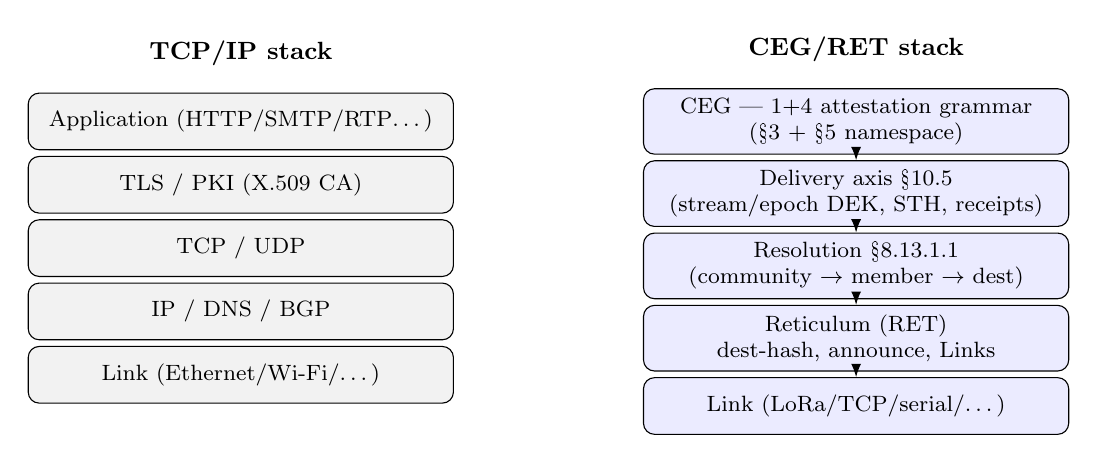
\begin{tikzpicture}[node distance=2pt,
  layer/.style={draw,rounded corners,minimum width=5.4cm,minimum height=0.72cm,align=center,font=\footnotesize},
  ceg/.style={layer,fill=blue!8}, ip/.style={layer,fill=black!5}]
\node[ip] (app2) {Application (HTTP/SMTP/RTP\ldots)};
\node[ip,below=of app2] (tls) {TLS / PKI (X.509 CA)};
\node[ip,below=of tls] (tcp) {TCP / UDP};
\node[ip,below=of tcp] (ip) {IP / DNS / BGP};
\node[ip,below=of ip] (link2) {Link (Ethernet/Wi-Fi/\ldots)};
\node[font=\small\bfseries,above=6pt of app2] {TCP/IP stack};
\node[ceg,right=2.4cm of app2] (ceg) {CEG --- 1+4 attestation grammar\\(\S3 + \S5 namespace)};
\node[ceg,below=of ceg] (deliv) {Delivery axis \S10.5\\(stream/epoch DEK, STH, receipts)};
\node[ceg,below=of deliv] (res) {Resolution \S8.13.1.1\\(community $\rightarrow$ member $\rightarrow$ dest)};
\node[ceg,below=of res] (ret) {Reticulum (RET)\\dest-hash, announce, Links};
\node[ceg,below=of ret] (link3) {Link (LoRa/TCP/serial/\ldots)};
\node[font=\small\bfseries,above=6pt of ceg] {CEG/RET stack};
\draw[-Latex] (ceg)--(deliv); \draw[-Latex] (deliv)--(res); \draw[-Latex] (res)--(ret); \draw[-Latex] (ret)--(link3);
\end{tikzpicture}
\end{center}

\noindent Trust is intrinsic (signed quorum), not bolted on: \textbf{PKI/CA $\rightarrow$ hybrid
signatures + founder-quorum}; \textbf{DNS $\rightarrow$ \texttt{resolve\_community}};
\textbf{A-record $\rightarrow$ signed \texttt{transport\_destination}}; \textbf{IP routing
$\rightarrow$ RET announce/path-request}.

\subsection*{0.2 Per-message PQC sizes (derived)}
\begin{center}\footnotesize
\begin{tabular}{|l|r|l|}\hline
\textbf{Object} & \textbf{Bytes} & \textbf{Composition}\\\hline
Hybrid epoch-DEK grant (v2) & 4{,}669 & X25519 32 + ML-KEM-768 ct 1088 + wrapped DEK 48 + hybrid sig 3373 + env 128\\\hline
Per-stream STH & 3{,}485 & root 32 + sizes 16 + log\_id 64 + hybrid sig 3373\\\hline
AES-GCM tag / 1 MiB chunk & 16 & 0.0015\% content overhead\\\hline
ML-DSA-65 sig / Ed25519 sig & 3{,}309 / 64 & FIPS 204 / RFC 8032\\\hline
ML-KEM-768 ciphertext & 1{,}088 & FIPS 203\\\hline
\end{tabular}
\end{center}

\subsection*{0.3 Findings}
\begin{enumerate}\setlength\itemsep{2pt}
\item \textbf{PQC is not the bandwidth bottleneck --- content fan-out is.} The
AES-256-GCM content overhead is 0.0015\% at a 1 MiB chunk. At scale the dominant
cost is unicast content replication (e.g.\ $\sim$2 Tbps for 1M viewers at 2 Mbps),
which is the CDN / broadcast-relay-tree problem (1.x), independent of crypto.
\item \textbf{The PQC ``long tail'' is the per-rekey key cascade under churn ---
and \emph{removal coalescing}, not delivery topology, is what makes it
affordable.} Each \emph{gated-roster} member-removal forces an epoch rotation
(\S10.5.3 forward-secrecy). \textbf{Churn honesty (1.0-RC1 correction, \#71 C1):}
earlier drafts modeled churn$=$3{,}600/hr at N$=$1M (0.36\%/hr) --- $\sim$2 orders
below realistic broadcast-audience churn ($\sim$30\%/hr). At 30\%/hr with naive
per-removal rotation the flat-unicast cascade is $\sim$\textbf{3.1 Tbps ---
exceeding the $\sim$2 Tbps content fan-out itself}; the ``cascade $<$2\% of
content'' headline does NOT survive realistic churn unmitigated. The normative
mitigations (\S10.5.3): \textbf{(i) removal coalescing} --- all removals within
one STH window (T$=$2 s) batch into ONE rotation, capping the epoch rate at 1/T
\emph{regardless of churn} ($\leq$1{,}800 epochs/hr $\rightarrow$ $\sim$18.7 Gbps
flat-unicast at N$=$1M, $\sim$0.9\% of content fan-out; removed-viewer exposure
$\leq$ 2 s --- the grain the equivocation window already accepts); \textbf{(ii)
the public-broadcast exemption} --- an ungated \texttt{listed:public} roster has
no confidentiality claim against departed viewers, so removal forces no rotation
at all. With coalescing the three delivery regimes (hybrid grant 4.56 KiB;
TreeKEM commit $\sim$1.2 KiB/node, depth$=$20) keep their shape: \textbf{(a)
flat, unicast --- O(N) --- $\sim$18.7 Gbps} (the 1.0 shape); \textbf{(b) tree,
multicast --- O(log N) --- $\sim$0.1 Mbps} --- the 1.x lever, \emph{cheap only if
efficient multicast exists}; \textbf{(c) tree, unicast --- O(N log N) --- WORSE
than flat.} The tree's advantage remains multicast aggregation; whether efficient
multicast exists over the mesh is the open transport question of \S0.4.
\emph{(Two published self-corrections now stand in this item: the
$\log^2$/15 Mbps asymptotic error, and the 3{,}600/hr churn understatement ---
both caught in review, both kept on record per the \S1.4 honesty discipline.)}
Fig.~\ref{fig:cascade}.
\item \textbf{Lag is transport-bound, not crypto-bound.} Per-chunk AES seal/open
is $\sim$$\mu$s; the ML-KEM-768 DEK decap is $\sim$30 $\mu$s \emph{once per epoch}.
Glass-to-glass lag is dominated by chunk/segment duration, STH cadence (T=2s for
accountable broadcast), and \textbf{Reticulum Link RTT}. Fig.~\ref{fig:lag}.
\item \textbf{Join cost is dominated by RNS path-setup, not the handshake.} The
hybrid KEX (ML-KEM encap+decap) + signature verify are sub-millisecond; RNS path
establishment is the variable. Fig.~\ref{fig:join}.
\end{enumerate}

\subsection*{0.4 Do we have enough detail? (yes, parametrically)}
\textbf{Sufficient and pinned:} all crypto sizes (FIPS 203/204, RFC 8032), the
AES-GCM chunk overhead, cadence constants (K=64, T=2s, MAX\_CHUNKS/epoch=$2^{24}$,
1 MiB chunk), and cascade complexity (flat O(N), tree O(log N) with multicast, O(N log N) without).
\textbf{Parametric (RC1-7 unratified):} K, T, MAX\_CHUNKS --- the model is a
function of them. \textbf{The one missing empirical input:} Reticulum transport
characteristics (Link RTT, throughput, MTU, path-setup time) per interface ---
CEG defers transport to RET, so the lag term is a free parameter. Over IP-backed
RNS, assume $\sim$internet RTT + small RNS overhead (realtime video feasible);
over LoRa, seconds (realtime infeasible; store-and-forward only). \textbf{To go
parametric $\rightarrow$ concrete, measure RNS Link RTT/throughput on the target
interfaces.} The O($\log$N) tree (1.x) and SFU relay (1.x) are modelled with
standard complexity, not yet spec-detailed.

\subsection*{0.5 Comparison to other PQC streaming proposals}
The modern E2E-media stack the industry is converging on is \textbf{MLS (group key,
TreeKEM) + SFrame (per-frame AEAD) + hybrid-PQC KEM + PQC-TLS transport}; the
crypto trio everyone lands on is \textbf{ML-KEM-768 + ML-DSA-65 + AES-256-GCM}
(Zoom's shipped PQC E2EE; the Frontiers 2025 authenticated-PQC-session paper;
NIST FIPS 203/204). \textbf{CEG \S10.5 is structurally the same stack} --- we
independently arrived at the converged design, which is the strongest validation
of the crypto choices.

\begin{center}\scriptsize
\begin{tabular}{|p{2.6cm}|p{2.4cm}|p{2.4cm}|p{2.4cm}|p{3.2cm}|}\hline
 & \textbf{Zoom PQC E2EE} & \textbf{MLS+SFrame (IETF)} & \textbf{WebRTC DTLS-SRTP} & \textbf{CEG \S10.5} \\\hline
KEM & ML-KEM-768 & hybrid ML-KEM (agile) & (PQ-DTLS exploratory) & \textbf{hybrid X25519+ML-KEM-768} \\\hline
Per-frame AEAD & AES-GCM & AES-GCM / CTR+HMAC & SRTP & AES-256-GCM (STREAM nonce) \\\hline
Group rekey & key tree & \textbf{TreeKEM O(log N)} & n/a (SFU sees plaintext) & flat O(N) 1.0 $\rightarrow$ MLS-tree (RFC 9420) 1.x, multicast-dependent \\\hline
Transparency log & none & none & none & \textbf{per-stream STH (RFC 6962) + receipts} \\\hline
Identity / trust & Zoom accounts & app-supplied & X.509 / fingerprints & federation keys + founder-quorum, DNS-free \\\hline
Topology & central SFU & delivery-service & SFU/P2P & RET mesh, no central server \\\hline
Maturity & \textbf{shipped at scale} & \textbf{standardized} & \textbf{battle-tested} & pre-1.0 \\\hline
\end{tabular}
\end{center}

\noindent\textbf{Where CEG is unique:} it composes media with the federation's
transparency log + identity + governance + payments under \emph{one} grammar
(the same 1+4 set), DNS-free over RET, no central server or CA --- the per-stream
STH (anti-equivocation: a producer can't show different chunk-K to different
viewers), delivery receipts, and settlement linkage have no equivalent in
Zoom/MLS/SFrame. \textbf{Where CEG is behind (honest):} MLS \emph{ships} TreeKEM
today (our O(log N) tree is 1.x); Zoom \emph{ships} PQC E2EE at scale; WebRTC's
transport is battle-tested where RNS realtime media is unproven (our open
RTT question). \textbf{Crib list} (\S0.7): adopt MLS TreeKEM (RFC 9420) verbatim
for the 1.x tree rather than reinvent; consider SFrame framing to ride
standardization; revisit the forward-only (no-PCS) choice against MLS's PCS.

\subsection*{0.6 Concrete numbers from a transport profile}
Feeding representative transport assumptions into the model (\texttt{concretize.py};
replace with \texttt{rns\_transport\_bench.py} measurements):
\begin{center}\footnotesize
\begin{tabular}{|p{4.6cm}|r|r|r|l|}\hline
\textbf{transport (RTT)} & \textbf{realtime call} & \textbf{broadcast} & \textbf{join} & \textbf{verdict}\\\hline
IP-backed RNS, same region (35 ms) & 115 ms & 2.4 s & 71 ms & interactive-grade\\\hline
IP-backed RNS, cross-region (140 ms) & 220 ms & 2.5 s & 282 ms & OK ($<$400 ms)\\\hline
LoRa SF7 (1.2 s) & 1280 ms & 3.6 s & $\sim$10 s & store-and-forward only\\\hline
\end{tabular}
\end{center}
\noindent Over IP-backed RNS, PQC realtime video is interactive-grade; the crypto
contributes sub-millisecond. (Illustrative pending real RNS measurement.)

\subsection*{0.7 Per-operation benchmark + crib findings}
Measured here (pyca/cryptography); PQC rows from published liboqs (AVX2);
cross-check target = ciris-crypto \texttt{benches/federation\_crypto.rs}.
\begin{center}\footnotesize
\begin{tabular}{|p{5.2cm}|r|r|l|}\hline
\textbf{operation} & \textbf{$\mu$s/op} & \textbf{wire B} & \textbf{source}\\\hline
X25519 ECDH & 23.2 & 32 & measured\\\hline
Ed25519 sign / verify & 20 / 69 & 64 & measured\\\hline
AES-256-GCM seal/open (1 MiB) & 144 / 141 & +16/chunk & measured (58 GB/s)\\\hline
ML-KEM-768 encaps / decaps & $\sim$30 / $\sim$25 & ct 1088 & liboqs\\\hline
ML-DSA-65 sign / verify & $\sim$330 / $\sim$110 & sig 3309 & liboqs\\\hline
\end{tabular}
\end{center}
\noindent\textbf{The headline that answers ``isn't PQC slow E2E?'':} PQC
\emph{compute} is comparable to classical (ML-KEM encaps $\sim$30 $\mu$s $\approx$
X25519 23 $\mu$s); the cost is \emph{size} ($\sim$30--50$\times$). And CEG puts the
asymmetric PQC on the per-\emph{epoch} cold path while every \emph{frame} rides
AES-256-GCM ($\sim$58 GB/s, PQC-safe). ``PQC is slow E2E'' conflates size with
compute; the KEM-then-symmetric placement (same as TLS-bulk, MLS+SFrame) defeats
it. \textbf{Cribbed gotchas:} (1) \emph{multi-sender nonce reuse} --- in group
video N senders share an epoch but each emits its own \texttt{stream\_id}, so the
STREAM nonce prefix HKDF(epoch\_dek; stream\_id, epoch) is per-sender-unique
(SFrame solves the same hazard with per-sender keys; our per-sender stream\_id is
equivalent --- now explicit). (2) \emph{TreeKEM unmerged-leaves / double-join} ---
adopt RFC 9420 handling wholesale in the 1.x tree. (3) \emph{PCS} --- MLS offers
post-compromise security via key-updates; CEG chose forward-only (Option A);
flagged for reconsideration.

\begin{figure}[h]\centering
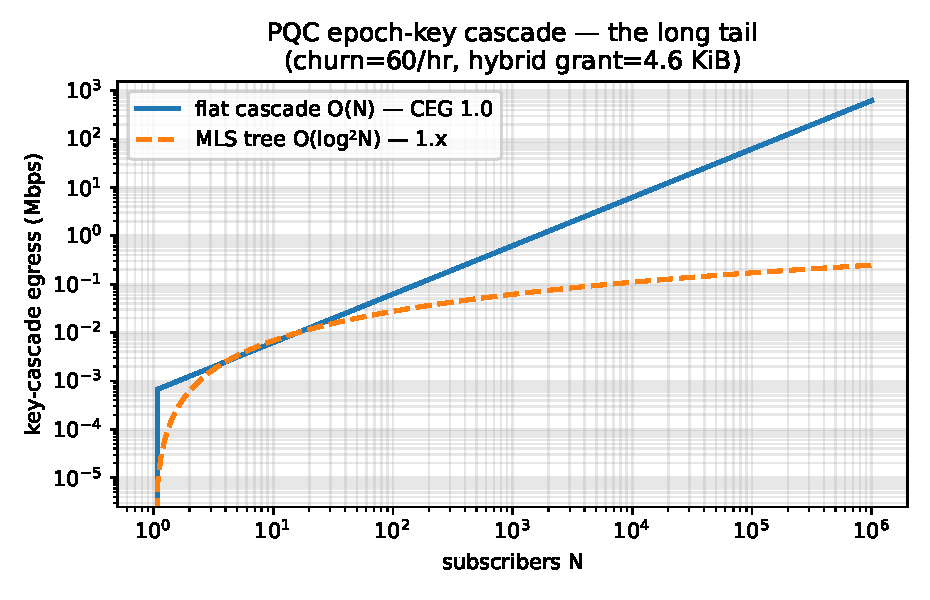
\includegraphics[width=0.78\textwidth]{fig_cascade.pdf}
\caption{Per-rekey PQC key cascade vs N under three delivery models. The tree wins ONLY with efficient multicast (b); without it (c) it is worse than flat. Delivery, not complexity, is decisive.}\label{fig:cascade}
\end{figure}
\begin{figure}[h]\centering
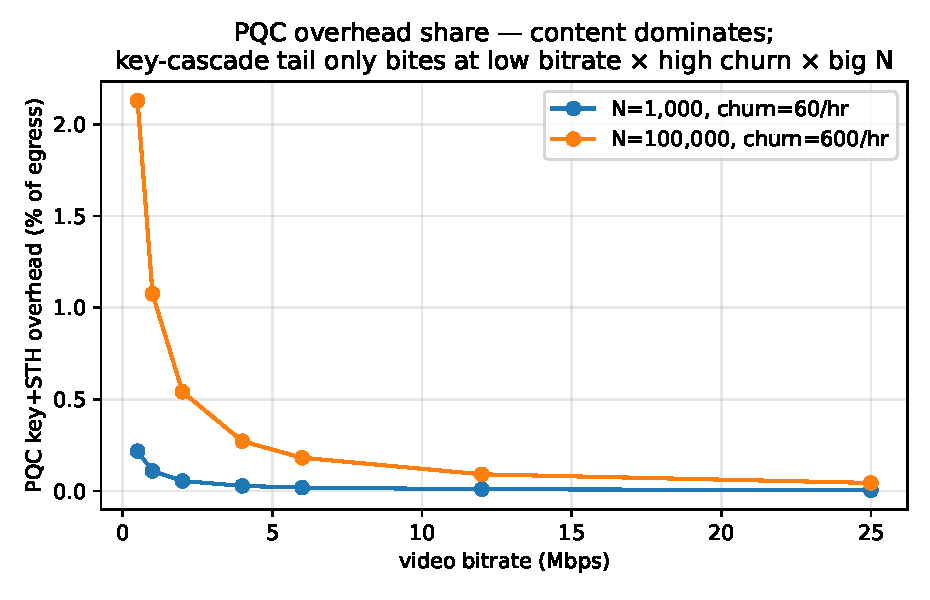
\includegraphics[width=0.70\textwidth]{fig_overhead.pdf}
\caption{PQC key+STH overhead as a share of egress --- content dominates; the key tail bites only at low bitrate $\times$ high churn $\times$ huge N.}\label{fig:overhead}
\end{figure}
\begin{figure}[h]\centering
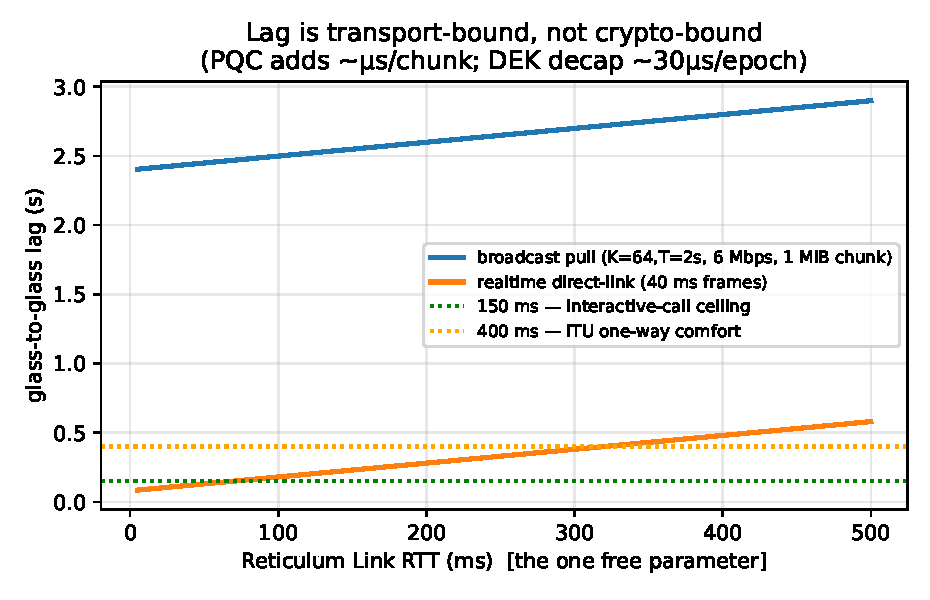
\includegraphics[width=0.78\textwidth]{fig_lag.pdf}
\caption{Glass-to-glass lag vs Reticulum Link RTT (the free parameter). PQC adds $\sim\mu$s; transport sets the regime.}\label{fig:lag}
\end{figure}
\begin{figure}[h]\centering
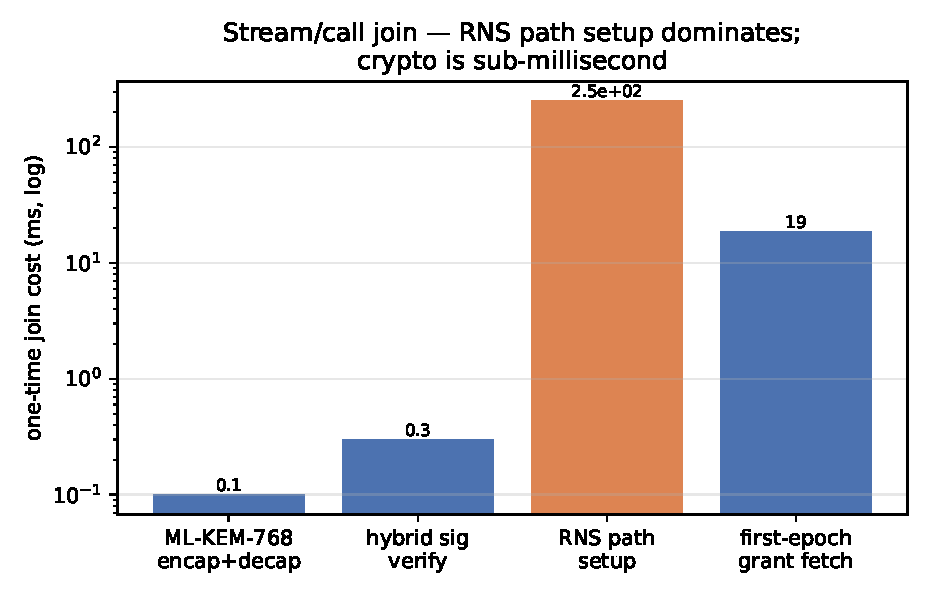
\includegraphics[width=0.70\textwidth]{fig_join.pdf}
\caption{Stream/call join one-time cost --- RNS path setup dominates; crypto is sub-millisecond.}\label{fig:join}
\end{figure}
\clearpage

\section*{CEG — The CIRIS Epistemic Grammar}


\textbf{Version}: 1.0-RC4 (Release Candidate — wire surface FROZEN; design surface COMPLETE; §RC ratified)

\textbf{Status}: Release Candidate (2026-06-10). \textbf{The wire surface is frozen} (since RC1) and — with this cut — \textbf{the design surface is complete}: the \#70 operational-data subject\_kinds were the one scheduled addition, and they have now landed additively (§5.6.8.13 + §10.1.6, the §1.4 sixteenth path) after three-sided federation review (Edge/Verify/Persist). \textbf{No further additions are scheduled.} Implementers SHOULD pin RC4; any change between RC4 and 1.0 is a \textbf{found defect}, not design. The \textbf{1.0 label} waits on the \#57 freeze gate: streaming substrate shipped (CIRISPersist\#142), Spock removed (\#58), conformance artifacts (OpenAPI + \texttt{dimensions.json}) generated from these frozen shapes, and \textbf{one full implementation cycle across Persist + NodeCore + Lens + Agent + Edge with no new wire-break}. That silence is the freeze signal; 1.0 is these bytes re-tagged.


\textbf{RC2 → 1.0 — what actually remains (sharpened by the substrate-side dependency review, 2026-06-12).} With persist having consumed RC2's hard surfaces (§5.6.8.13/§10.1.6 operational data, §5.6.8.8.2 three-role identity, §0.9 JCS), the spec-side residual is now \textbf{one conformance push} (the one ratification landed in RC4 — see below):

\begin{enumerate}\setlength\itemsep{0pt}
\item ✅ **RATIFIED in RC4 — the \texttt{consent\_role} §RC slot is filled** (new §7.0.2; CIRISAgent\#760 OQ-1/2/3 all closed at the \texttt{ConsentGate.lean} defaults, with the permissive OQ-1 audit clause). The \texttt{consent\_role} JSONB shape is \textbf{locked} (flat, non-recursive, overwrite-on-revoke; chain history never embedded), and implementations **MAY now build the \texttt{consent\_role} substrate\textbf{ — the CIRISPersist\#146 consent-SLA watcher + schema and the CIRISEdge consent-gate are }unblocked\textbf{. }No CEG-spec decision remains open.** (Everything else cited as "gated on CEG 0.6/0.7/0.15" was already locked downstream build work.)
\item \textbf{The RC2→1.0 conformance gate — CIRISPersist\#171 four-impl conformance.} CEG reaches 1.0 only once Agent + NodeCore + LensCore + Registry all conform against persist's shared \texttt{federation\_attestations} surface. CEG-side prerequisite: the \textbf{local-tier attestation semantics (§10.1.3 / §11.9 / §7) frozen at 1.0} so persist can finalize the surface coherently. This is the gate where "RC2 vs 1.0" matters most.
\end{enumerate}


OQ defaults are \textbf{fail-secure-defaulted} (soft, non-blocking; a CEG confirm only locks the default): OQ-4 DEK-recovery tier → content-master self-retention grant; steward self-anchor / \texttt{root\_stewards} → per-region caller-supplied stewards behind a fail-closed authority resolver.


\begin{quote}\itshape \textbf{Human-reading edition:} \texttt{pdf/ceg-1.0-rc4-reader.pdf} is the de-editorialized, deduplicated, human-first cut (version history, per-path narrative, and provenance cross-refs stripped). This source tree remains the canonical working draft and retains that lineage.\end{quote}


**1.0-RC4 — §RC ratified: the \texttt{consent\_role} Counter-RII gate (Agent\#760 OQ-1/2/3; no wire change).\textbf{ The one reserved §RC slot is }filled** (new §7.0.2), ratifying the Accord §RC \texttt{consent\_role} semantics at the \texttt{ConsentGate.lean} defaults — \textbf{zero proof delta}: \textbf{(OQ-1)} revocation chain is \texttt{BaseRole}-only, non-recursive — overwrite-on-revoke, chain history (\textit{if retained}) lives in a separate audit surface and is **never embedded in the \texttt{consent\_role} JSONB\textbf{ (locks the substrate-portable shape; the permissive "if retained" is }non-breaking against the shipped flat soft-delete substrate\textbf{); }(OQ-2)** \texttt{Peer}-role nodes are blanket-suppressed from Counter-RII at any \texttt{trust\_mode} — bounded because \texttt{ratchet:flag:counter\_rii:\{layer\}} is \textbf{advisory-only} (§5.7), never sole evidence for \texttt{slashing:*} (WA quorum is the gate); \textbf{(OQ-3)} \texttt{AuthorizedReview} is \textbf{strict} (signal-eligible immediately past \texttt{window\_end}). With this the design surface has \textbf{zero open CEG decisions}, and the \texttt{consent\_role} substrate is unblocked (CIRISPersist\#146 back-half + the CIRISEdge consent-gate). \texttt{consent\_role} is a \texttt{federation\_keys} identity field (§7.0.1 sibling), not an envelope primitive — \textbf{no 1+4 change, no wire break.}


\textbf{1.0-RC3 — clarity cut (fabric-node trust model + NodeCode shorthand; no wire change).} Four clarifications + one canonical-encoding addition, all additive on the frozen surface: \textbf{(1)} §7.0.1 the \textbf{fabric-node separation-of-powers} — a fabric node (the headless cohabitation runtime; \texttt{agent = fabric node + brain}) co-locating \texttt{\{substrate\_persist, steward, lenscore\_detector, witness, …\}} in one process is \textbf{custody, not consolidation of authority}: authority stays quorum-bound (a vote, not a verdict), observation stays non-authoritative by namespace (\texttt{detection:*}, validated-not-adjudicated), and \textbf{observation can never manufacture authority} (the "lenses become the gate" hazard is structurally unreachable). \textbf{(2)} §5.6.8.10 **\texttt{ciris-canonical} is a default, not a forced root\textbf{ — a conformant consumer MUST be able to }re-root\textbf{ (infrastructure is a general primitive; anyone may run their own canonical group; membership grows by founder-quorum vote; DNS is never in the trust/addressing chain) + }trust ≠ consent\textbf{ are distinct role-scoped relationships (trust = inbound acceptance of output; consent = outbound data-flow; lens trust=scores/consent=traces, registry trust-only, node consent medium-varied over }one** \texttt{consent:*} object). \textbf{(3)} New §0.10 \textbf{NodeCode} — the canonical \texttt{key\_id} shorthand encoding (\texttt{CIRIS-V1-…}, RFC 4648 base32 + CRC-16-CCITT, lifted from the shipped CIRISAgent codec per \#75) so every impl renders the same code for the same key; a deterministic render of an existing \texttt{key\_id}, \textbf{not} an envelope field. \textbf{(4)} README \textbf{RC2→1.0 residual} sharpened from the substrate dependency review (one open decision — \texttt{consent\_role}/§RC via Agent\#760; one conformance push — Persist\#171 four-impl). \textbf{No 1+4 change, no wire break.}


\textbf{1.0-RC2 — operational-data envelopes (the scheduled additive cut; design surface complete)} (per \#70, under the \#58 Spock-removal epic; three-sided review Edge/Verify/Persist — zero blockers, zero new structural primitives confirmed): cross-region operational Portal data becomes signed CEG envelopes. \textbf{Three new subject\_kinds} (§5.6.8.13): \texttt{organization} · \texttt{org\_membership} · \texttt{partner\_record} (the Edge v2 \texttt{EnvelopeKind} wire tokens; v2 \texttt{envelope\_hash} = \texttt{sha256(JCS(envelope))}). \textbf{Governing principle}: federate the trust/authz-minimal projection; PII + business detail stay region-local (Registry emit-side discipline — the substrate is not a PII filter). \texttt{User} records do NOT federate — only the role binding does. \textbf{Authority}: org/membership = single-signer role-gated (the §8.1.12.7.1 delegation resolver — never founder-quorum); \texttt{partner\_record} = \textbf{M-of-N steward quorum} (§5.6.8.10 machinery) with the \textbf{admission quorum ≠ merge quorum} distinction normative. \textbf{Determinism}: capability/restriction arrays are set-semantics→sorted (M signers must converge on identical JCS bytes \textit{before} the quorum evaluates — the highest-value pin); \texttt{revision: u64} monotonic anti-rollback per license. \textbf{New §10.1.6}: CEG-declared per-subject\_kind merge intents (\texttt{lww\_skew\_bounded}+\texttt{withdrawal\_forward\_only} / \texttt{monotonic\_quorum} V058-generalized) + the §0.7 skew-bound at admission (closes the LWW role-escalation surface). \textbf{Stable-id resolution} (not chain-walk — partition tolerance); first-class indexed business-id columns. \textbf{No payment-processor data, normative + fail-secure.} Sixteenth path; no 1+4 change. Unblocks \#58 Phase 3 (de-Spock) + Edge v2 + Persist \texttt{put\_*} surfaces.


\textbf{1.0-RC1 — the freeze cut} (per \#71 backwards-pass + CIRISVerify\#64 + \#57 blocker A): five honesty/safety patches + two pins + the canonical-bytes resolution, then freeze. \textbf{(C1)} §10.5.3 \textbf{removal coalescing} (all removals in one STH window T=2s batch into ONE rotation — caps the cascade at 1/T regardless of churn; the original model's 3,600/hr churn understated realistic broadcast churn \textasciitilde{}2 orders: naive 30\%/hr at N=1M ≈ 3.1 Tbps > the 2 Tbps content fan-out; coalesced ≈ 18.7 Gbps ≈ 0.9\%) + the \textbf{public-broadcast exemption} (ungated \texttt{listed:public} rosters: removal forces no rotation — no confidentiality claim against departed viewers). \textbf{(C2)} §5.6.8.8.2 forward-secrecy honesty: KEM rotation bounds \textit{future} exposure only; historical-content recovery requires DEK rotation + re-encryption, which is NOT mandated — named gap. \textbf{(C3)} §10.1.4 fail-secure exclusion is no longer silent: new §7.7 \texttt{hard\_case:recipient\_excluded:\{scope\}} emitted INTO the affected cohort (never federates beyond). \textbf{(C4)} §5.6.8.8.2 admission MUST-reject content-KEM x25519 == transport x25519. \textbf{(C5)} §9.1 names the two-holders-one-household correlated-failure geometry; authority is the full constitutional kill; the mitigant is \textbf{finding new holders} (active obligation). \textbf{Pins}: §0.9.2.1 base64 = RFC 4648 STANDARD padded (protocol-layer pin; CIRISVerify\#64); ML-KEM-768 pubkey = exactly 1184 B; \texttt{encryption\_pubkeys} joins the §8.1.12.7.1 member set (c); §5.6.8.4 crypto-agility headroom note (v3/ML-KEM-1024 additive). \textbf{Blocker A closed}: §5.2.1 provenance contracts redesigned to **JCS (RFC 8785) objects with pinned \texttt{domain} members\textbf{ — TupleHash128 retired (one canonicalization family); v1 newline forms deprecated-historical; §9.2.1 accord invocation intentionally unmigrated (closed-vocabulary preimage). }No 1+4 change.**


\textbf{0.18 — recipient encryption-key registration} (per CIRISRegistry\#69 + CIRISPersist\#192): the §10.1.4 substrate-wraps DEK cascade (the 0.17 community + self/family tiers all rely on it) needs each recipient's \textbf{content-encryption} keys (x25519 + ML-KEM-768) — but the federation directory carries only \textbf{signing} keys (Ed25519 + ML-DSA-65), and ML-KEM is not derivable from ML-DSA. 0.18 adds the optional **\texttt{encryption\_pubkeys} field-set on \texttt{identity\_occurrence}** (§5.6.8.8.2), structurally parallel to \texttt{transport\_destination}: self-certified (\texttt{attesting\_key\_id == identity\_key\_id}), hybrid-signed, \texttt{supersedes}-rotatable (rotate a KEM key without touching the signing identity), and \textbf{already cross-region-replicated inside the occurrence envelope} (\texttt{EnvelopeKind::IdentityOccurrence}, CIRISEdge\#65) — so \textbf{no new replication kind, no Edge wire change}. These feed \texttt{wrap\_algorithm: v2} directly (§5.6.8.4). Adds the \textbf{fail-secure-exclusion} rule (§10.1.4): a recipient whose occurrence carries no valid ML-KEM key is \textit{excluded} from the grant (content stays encrypted) — never a plaintext or v1 fallback. \textbf{Key separation (normative):} the content-KEM x25519 is distinct from the signing keys AND from the Reticulum transport x25519 — three purposes, three keypairs, never reused. \textbf{No 1+4 change} — one optional field-set on an existing subject\_kind (§1.4 fifteenth path).


\textbf{0.17 — the three crypto tiers} (per CIRISRegistry\#67; the line is \textit{"does it have a bounded membership roster?"}): the ≤0.16 binary cut (self/family encrypt; everything else plaintext) is replaced by \textbf{self/family} (encrypted + structurally invisible) → \textbf{Community} (\texttt{community} / \texttt{affiliations}: encrypted under a \textbf{per-community DEK} + \texttt{holds\_bytes:*} with cleartext provenance — byte-confidential to members, discoverable by provenance) → \textbf{Commons} (\texttt{species} / \texttt{biosphere} / \texttt{federation}: plaintext, anyone inspects). The community DEK \textit{is} the §10.5.3 epoch-DEK cascade (one shared DEK, O(1)/emission, v2/PQC mandatory) — \textit{"a community is a stream its members subscribe to, cryptographically"} — refuting the 0.8 "infeasible" premise. \textbf{Mandatory, not opt-in} (the tier name is the guarantee; a persecuted community is protected by \textit{being} one). Adds the \textbf{holder-inspectability principle} (§8.1.13.3: nothing above local tier is a forced unattributable opaque blob) + two rulings: \texttt{cohort\_subkind: infrastructure} communities (\texttt{ciris-canonical}/governance) are the \textbf{plaintext Commons exception} (the trust root must be inspectable), and node→canonical conformance traces are \texttt{cohort\_scope: federation} (world-readable). Overturns §8.1.13.4 (community now has the removed-member problem → Option-A re-key). \textbf{No 1+4 change} — the community DEK is the existing epoch cascade applied to \texttt{cohort\_scope: community}.


\textbf{0.16 is additive vs 0.15} — the agent-identity hardening + cross-impl byte-determinism wave (no wire-format change; all composition + canonicalization pins over the locked 1+4 set):

\begin{itemize}\setlength\itemsep{0pt}
\item \textbf{§10.1.5 attestation tier model} — \texttt{local} (deferred-signature, producer-only-authority) vs \texttt{federation} (hybrid-signed, visible) tiers + \texttt{promote} (local→federation) + the open-prefix \texttt{query}; the shared agent-facing attestation surface (CIRISPersist\#172). + §10.1.3 eligibility corrected to "revocation authority, not empty \texttt{subject\_key\_ids}".
\item \textbf{§8.1.12.7 "Self at login"} — one hybrid hardware-rooted user identity with app + agent occurrences sharing one Policy-L Self DEK, partnered + delegated to act on the user's behalf (CIRISRegistry\#65); + §8.1.12.7.1 signing member sets + \texttt{delegated\_scope} canonical kinds.
\item \textbf{§0.9.2.1 canonical-bytes determinism rules} — array element ordering (set vs sequence), byte-field→lowercase-hex (§0.6), timestamp→§0.5; the three things JCS doesn't pin (CIRISVerify\#63).
\item \textbf{PQC at rest extended to self/family} — §8.1.12.4 \texttt{wrap\_algorithm: v2} (X25519+ML-KEM-768) MANDATORY for the at-rest DEK cascade (was v1); §10.1.4 split into unconditional structural-invisibility + defense-in-depth at-rest encryption (CIRISPersist\#152).
\item \textbf{Standard-pins}: §10.5.2 STREAM-nonce \texttt{epoch} = 8-byte BE (\#63); §10.5.3/§5.6.8.4 \texttt{wrap\_algorithm: v2} wire string \texttt{x25519\_mlkem768\_aes256\_gcm\_hkdf\_sha256} (\#64).
\item \textbf{Hygiene}: §1.5→§1.6 (overloaded with the Recursive Golden Rule) + §15.6 duplicate-heading fixes.
\end{itemize}


\textbf{0.15 folds the streaming standards in fully} (per CIRISRegistry\#61): the §10.5 streaming surface now \textbf{conforms to} the published standards rather than gesturing at them — the per-frame seal conforms to \textbf{SFrame} (draft-ietf-sframe); the epoch-key rekey conforms to \textbf{MLS TreeKEM} (RFC 9420) with Post-Compromise Security now available (optional, operator-enabled); the delivery-model analysis (flat-unicast O(N) vs tree-multicast O(log N) vs tree-unicast O(N log N)) is carried normatively; and RFC 9420 / SFrame / FIPS 203 / FIPS 204 / RFC 9180 are added to the §0.4 normative references. \textbf{No wire-format change} — the streaming primitives are unchanged, now standards-anchored. Also: §0.1.1 normative-vs-informative demarcation, §1.6 adversary model + privacy non-goals, and the §1.4 honesty pass (inductive-not-closure + the named falsification target) shipped in the 0.14→0.15 hardening.


\textbf{0.14 is purely additive vs 0.13} (per CIRISRegistry\#59 + \#55): \textbf{CEG↔value-transfer linkage + an §0.8 H3 prose correction.} Value transfer is not a CEG primitive (it rides USDC-on-Base via x402 under Identity=Wallet); CEG 0.14 adds the **optional, privacy-scoped attestation that \textit{links} a federation action to its off-stack settlement\textbf{ — closing the last form of internet traffic from the completeness audit (commerce-relationship auditability). }One new subject\_kind** (§5.6.8.12) \texttt{settlement} (+ a \texttt{settlement:*} dimension family for the bare-\texttt{scores} shape; parallel to \texttt{consent\_record}/\texttt{key\_grant} primitive-vs-ceremony): \texttt{settled\_action\_ref} + \texttt{rail} + \texttt{settlement\_ref} (chain tx / x402 receipt, cited like an \texttt{evidence\_refs[]} blob) + optional \texttt{amount\_commitment} (cleartext OR hash/range). Self-authenticating via Identity=Wallet; \textbf{privacy-by-default} (\texttt{cohort\_scope: self}, §10.1.4 structural-invisibility applies), auditability opt-in (\texttt{cohort\_scope: public}); CEG records the receipt, the chain settles the value. Matches the converged 2026 SOTA (x402 receipt header + selective-disclosure privacy). \textbf{Plus a prose fix} (§0.8, per \#55): the H3 \texttt{cell\_id} resolution is decoded \textbf{via the H3 library} (resolution field bits 52–55), NOT the high 4 bits (which are the H3 mode marker) — the prior "high 4 bits encode resolution" wording contradicted the spec's own \texttt{8001fffffffffff} res-0 example; example + intent were correct, only the decoding description was wrong. \textbf{1+4 wire-format lockdown preserved} — \texttt{settlement} rides existing \texttt{scores} + subject\_kind discriminator; \texttt{settlement\_ref} rides existing \texttt{evidence\_refs[]}; visibility rides existing \texttt{cohort\_scope}. Zero new structural primitives. Fourteenth independent path on §1.4 — commerce-relationship auditability (the receipt, not the rail) as composition.


\textbf{0.13 is purely additive vs 0.12} (per CIRISRegistry\#56): \textbf{realtime group communication as composition.} The delivery axis (CEG 0.10) covered 1:1 observer-share and 1:N broadcast; CEG 0.13 documents that \textbf{group video, voice, desktop/screen sharing, text chat, and topic-scoped channels with sub-channels} are the \textit{same primitive set at N↔N cardinality} — composing from \texttt{community} + \texttt{live\_stream} (§10.5) + \texttt{chat\_message} + member/transport resolution (§8.1.13.1.1). \textbf{One new normative subsection} (§10.5.8) — the composition map (call/voice/screen-share/chat/channel/sub-channel/presence/invite) + a transport-profile extension: broadcast = pull-only (1.0) / relay-tree (1.x); \textbf{realtime small-medium group = direct Reticulum Links} (low-latency mesh, in 1.0 — no relay tree needed at small N); realtime large group = SFU relay (1.x). Ephemeral call = short-lived \texttt{community}; persistent channel = long-lived \texttt{community}. PQC unchanged + mandatory (epoch DEK \texttt{wrap\_algorithm: v2}; hybrid KEX transit). \textbf{1+4 wire-format lockdown preserved} — zero new structural primitives; the entire realtime-collaboration surface is composition over already-locked primitives. Thirteenth independent path on §1.4 — the most product-complete confirmation: a full group-communication platform needs nothing beyond the 1+4 set + the delivery axis + community membership.


\textbf{0.12 is purely additive vs 0.11} (per CIRISRegistry\#56 + CIRISEdge\#15): \textbf{the DNS-free addressing layer — authenticated member resolution for a CEG/RET stack.} With Spock removed and replication CEG-native (CIRISRegistry\#58), the federation speaks \textbf{CEG over Reticulum, not TCP/IP} — so resolving "who is in a community and how do I reach them" cannot lean on DNS. CEG 0.12 locks that resolution as a chain of signed bindings: \textbf{one new optional field} \texttt{transport\_destination} on \texttt{identity\_occurrence} (§5.6.8.8.1) — a federation-key-signed binding of a Reticulum dual-key transport destination (\texttt{hash(x25519‖ed25519)}) to an identity, closing AV-42 (spoofed transport↔identity binding) and promoting CIRISEdge\#15 Option B into a first-class auditable CEG shape; \textbf{one new normative resolution section} (§8.1.13.1.1) — deterministic \texttt{resolve\_community} (pinned \texttt{now} / latest / ordering / founder-subset eval) + \texttt{resolve\_member\_transport} (WHO via signed quorum · BINDING via signed occurrence · WHERE via Reticulum) + the cold-start rule (pin \texttt{community\_key\_id} + seed destinations; reachability ≠ trust). \textbf{1+4 wire-format lockdown preserved} — one optional field on an existing subject\_kind + an evaluation algorithm over existing fields; zero new structural primitives. Twelfth independent path on §1.4 — the wire format expresses \textbf{its own addressing/naming layer}, DNS-free and self-certifying.


\textbf{0.11 is purely additive vs 0.10} (per CIRISRegistry\#56): **\texttt{cohort\_subkind: infrastructure} — the trust-root community subkind.** CEG 0.8 codified \texttt{community} with one subkind (\texttt{geographic}, admission-over-current-members + \texttt{location\_proof} gate). The CIRIS canonical services (Registry / Lens / Node) need a community that is governed as a \textit{trust root}, not a city: no location gate, and admission evaluated over the \textbf{founder} subset rather than all members (the anti-Sybil guardrail — flooding the membership must not dilute the admission quorum). CEG 0.11 codifies the second canonical \texttt{cohort\_subkind} (§5.6.8.10 "Canonical \texttt{cohort\_subkind: infrastructure}"): one \texttt{infrastructure\_constraint} payload (\texttt{service\_class} + \texttt{admission\_quorum\_basis: "founders"}) + trust-root conformance requirements (\texttt{consensus\_protocol} MUST be \texttt{quorum:M/N}; \texttt{consensus\_protocol\_entrenched} MUST be \texttt{true}; the founder-subset evaluation basis). This is the shape the \texttt{ciris-canonical} trust root adopts instead of a \texttt{family} (rationale: \texttt{CIRISRegistry/MISSION.md} §2.1.1 — public content model, decentralization ramp, legitimacy). \textbf{1+4 wire-format lockdown preserved} — one open-vocab \texttt{cohort\_subkind} value + one optional payload shape; admission rides existing \texttt{consensus\_protocol} + \texttt{supersedes}; the founder-subset basis is an evaluation rule over the existing \texttt{role} field, not a new structural primitive. Eleventh independent path on §1.4.



The load-bearing insight at CEG 0.10: \textbf{observer-share (N=1) and streaming multicast (N>1) are the same primitive at different cardinality} — subscriber-set = \texttt{community} per Policy M; E2E directed delivery = \texttt{key\_grant} cascade of stream-epoch DEK over the roster. No special-case primitive for streaming, no special-case primitive for observer-share. The wire format's structural set is rich enough for substrate-fan-out and 1:N media multicast without any addition to the 1+4 set. Tenth independent path on §1.4.


\textbf{Bifurcated landing}: observer-share half ships \textbf{impl-live} (no remaining blockers per §15.6 RC1 register; Persist V054 confirmed; Edge E1-E4 locked; KEY\_GRANT\_V1\_INFO confirmed at \texttt{CIRISVerify/src/ciris-crypto/src/key\_grant.rs:71}); streaming multicast half ships \textbf{spec-now / impl substrate-pending} — best-effort tier pending CIRISPersist\#142 (unowned/unscheduled), accountable tier additionally pending CIRISRegistry\#34 (STH consistency-proof enforcement). Open coupling caveat \textbf{RC1-1c}: the V054 cross-column CHECK requires content-addressed \texttt{key\_grant}s; the §10.5.3 epoch-key axis needs a \textbf{parallel CHECK arm migration} at Persist — a bounded constraint migration, NOT pure-additive at the Persist constraint layer. Operational ratification \textbf{RC1-7} (constants \texttt{K=64} / \texttt{T=2s} / cosign per-epoch / \texttt{MAX\_CHUNKS\_PER\_EPOCH=2²⁴} + Policy E accountable quorum) pending; operator-tunable, not blocking spec ship.


\textbf{rotation\_chain hygiene corrections} folded in: CEG 0.3's \texttt{key\_grant.rotation\_chain} is the \textbf{content-addressed grant-supersession lineage} (per §5.6.8.4 disambiguation), NOT a key-rotation primitive on its own. CEG 0.10 §10.5.3's per-\texttt{(stream\_id, epoch)} epoch-key axis reuses the same payload-level supersession mechanism on a \textbf{separate parallel addressing axis}. Prior CEG text (§11.7.1, §1.4 path-8) wrongly framed \texttt{rotation\_chain} as covering DEK rotation; corrected here.


\textbf{0.9 carries one wire-break vs 0.8} (per CIRISRegistry\#49 + CIRISAgent\#856): **\texttt{federation\_keys.identity\_type} becomes a SET of roles — single-key role cohabitation.** Every §7 reserved-prefix emitter rule is now evaluated by set membership (\texttt{X ∈ identity\_type}) rather than scalar equality. A single federation key MAY hold multiple roles at once — e.g. a folded CIRISAgent occurrence whose key is BOTH \texttt{agent} AND \texttt{lenscore\_detector} (§7.4), or a steward key that is both \texttt{substrate\_persist} and \texttt{witness}. This unblocks the CIRISAgent / LensCore fold-in (one key, many roles) which §7.4's scalar gate had blocked.


The wire-break is \textbf{representation-only and semantically null for legacy keys}: a pre-0.9 scalar \texttt{identity\_type="X"} is the singleton set \texttt{\{X\}}, so for any single-role key \texttt{X ∈ \{X\}} ≡ \texttt{X == X} and every pre-0.9 gating decision is unchanged. It is the second 0.x wire-break after the §0.2 attestation-ladder rename. \textbf{Zero new structural primitives, subject\_kinds, envelope fields, or §5 dimension prefixes} — the 1+4 wire-format lockdown is untouched; 0.9 is a §7-layer enforcement-rule generalization, NOT a §1.4 "Nth path" namespace addition. The capacity self-emission (§7.5), reasoning-trace, and agent-intent / LensCore-envelope-split resolutions from CIRISAgent\#856 are recorded as settled in §11.9. \textbf{One new conformance subsection} (§7.0.1), \textbf{one new governance section} (§11.9).


\textbf{0.8 is additive at the envelope layer vs 0.7} (per CIRISRegistry\#48): **\texttt{community} subject\_kind + \texttt{location\_proof} subject\_kind + \texttt{cohort\_subkind: geographic} discriminator + wire-format-enforced rough-only location precision.**


CEG 0.7 codified self/family membership; CEG 0.8 extends the membership story to the next scale — \textbf{communities} — with explicit admission semantics. Sibling subject\_kind to \texttt{family} but with different defaults: content scoped \texttt{cohort\_scope: community} \textbf{federates within the cohort} (emits \texttt{holds\_bytes:sha256:*} per status quo); there is NO at-rest DEK cascade; §10.1.4 structural-invisibility applies to self/family only. Communities scale up; families stay private.


The load-bearing privacy primitive at CEG 0.8 is the **\texttt{location\_proof} subject\_kind\textbf{ + the }§0.8 H3 cell canonicalization with rough-only enforcement (\texttt{cell\_resolution ≤ 7})**. Joining a geographic community is a one-way opt-in disclosure of rough location; the substrate enforces the precision bound at the wire format, so a producer cannot accidentally over-share even if the client UI fails to gate. Per ciris.ai/cewp, this is the structural-not-policy framing applied to geospatial disclosure: rough is rough by protocol.


\textbf{Two new subject\_kinds}, \textbf{one new envelope field} (\texttt{community\_id} required iff \texttt{cohort\_scope == community}; parallel to \texttt{family\_id}), \textbf{one new canonicalization section} (§0.8 H3 cell + rough-only resolution bound), \textbf{four new substrate-emitted reserved prefixes} (§7.8), \textbf{one new composition policy} (§8.1.13 Policy M), \textbf{one new governance section} (§11.8 geographic-community privacy invariant). Zero new structural primitives. Ninth independent path confirming the 1+4 minimal-and-adequate claim (§1.4) — and the most surprising path so far, demonstrating that \textbf{precision-bounded geospatial constraints can be expressed as canonicalization rules} (parallel to lowercase-hex per §0.6 or millisecond-precision datetime per §0.5), not as new structural primitives.


The composition unlocks \textbf{civic engagement + emergency messaging} as worked examples (§5.6.8.10 tables): neighborhood associations, municipal communities, voting districts, town halls, ballot initiatives, public comments, petitions, public-official self-attestation, FOIA requests, citizen-journalist coverage, whistleblower disclosure, civic mutual-aid networks; severe weather warnings, AMBER alerts, shelter-in-place orders, disease outbreak alerts, mass casualty incident coordination, infrastructure failure notices, disaster recovery activation, and the CONSTITUTIONAL-level halt path (the §9 HUMANITY\_ACCORD primitive that CEG 0.7 retconned as the canonical entrenched-\texttt{family} instance). All compose from the existing 1+4 set + the namespace additions.


\textbf{0.7 is additive at the envelope layer vs 0.6} (per CIRISRegistry\#47 + CIRISPersist\#152 + ciris.ai/cewp structural-invisibility framing): \textbf{self/family membership primitives + wire-format-level structural invisibility for self/family content.}


CEG ≤ 0.6 had no wire-format primitive linking multiple devices/agents to a single logical identity, nor any primitive expressing multi-key collectives like households. CEG 0.7 adds both — **\texttt{identity\_occurrence}\textbf{ (§5.6.8.8; self = trusted devices + agents) and }\texttt{family}** (§5.6.8.9; a group of trusted nodes with a per-family \texttt{consensus\_protocol} governing admission). Both ride existing \texttt{scores} + subject\_kind discriminator; both compose with existing structural primitives (\texttt{supersedes} for membership changes; \texttt{key\_grant.rotation\_chain} for DEK cascade on new-member admission).



\begin{quote}\itshape Self and family content never emits the attestation that would tell the rest of the network it exists. You don't need a privacy policy to keep family photos off the federation — the wire format can't carry them in the first place.\end{quote}


\textbf{New governance section} (§11.7) locks the four open decisions from \#47: Option A forward-secrecy (once shared, always shared at the wire layer; rotation deferred), envelope \texttt{family\_id} for multi-family disambiguation, reserved-prefix substrate ownership, and (the most consequential) **family admission requires consensus per the family's chosen \texttt{consensus\_protocol}** — NOT single-vouch — with six canonical protocols (\texttt{founder\_only} / \texttt{unanimous} / \texttt{majority} / \texttt{quorum:M/N} / \texttt{weighted:\{rubric\}} / \texttt{custom:\{id\}}) and meta-amendment via the protocol's own rules unless \texttt{consensus\_protocol\_entrenched}. Self-occurrence admission remains single-vouch (Signal-style trust-cascade per §11.7.4).


\textbf{Retcon at §9.1}: HUMANITY\_ACCORD triple is the canonical entrenched-\texttt{family} instance (3 founders, \texttt{consensus\_protocol: quorum:2/3}, \texttt{consensus\_protocol\_entrenched: true}). The constitutional asymmetry is "an entrenched family that is wire-scope-isolated to halt authority," not a one-off primitive.


\textbf{1+4 wire-format lockdown preserved} — zero new structural primitives. Two new subject\_kinds + one new envelope field + four new reserved substrate-emission prefixes + one new composition policy + one new endpoint discipline + governance section + §9 retcon. Eighth independent path confirming the 1+4 minimal-and-adequate claim (§1.4) — demonstrates the structural set is rich enough to express collective-scale membership AND the wire-format-level closure of the cewp structural-invisibility privacy claim.


\textbf{0.6 is additive at the envelope layer vs 0.4/0.5} (per CIRISRegistry\#45 + CIRISAgent\#842): \textbf{subject-side consent authority — the missing half of consent at the wire format.} Universal across medical records / photos / interviews / training data / group chat / financial / surveillance / FERPA-shape educational records / multi-party contracts. CEG ≤ 0.5 encoded only producer authority (\texttt{attesting\_key\_id}); CEG 0.6 adds subject authority via \textbf{one new optional envelope field} (§4.2): \texttt{subject\_key\_ids: Vec<KeyId>} — accepts both federation\_keys identities AND canonical-hash identifiers (resolves CIRISAgent\#840 OQ3 as side effect). Pre-0.6 producers omit the field; their Contributions stay in producer-only-authority shape. Pre-0.6 consumers that don't read the field see status-quo behavior.


**Semantic broadening of \texttt{withdraws}** (§3.2.3) to admit subject revocation + \texttt{delegates\_to} proxy chain for canonical-hash subjects; the primitive's wire shape is unchanged. \textbf{One new dimension family} (§5.6.8.6 \texttt{consent:*}) covering state / stream / deletion\_sla / deletion\_complete / decay / partnership\_grant / partnership\_accept / scope. \textbf{One new subject\_kind} (§5.6.8.7 \texttt{consent\_record}) — ceremony envelope parallel to \texttt{key\_grant} / \texttt{takedown\_notice}; both bare-\texttt{scores} and ceremony shapes admitted at the same gate. \textbf{New composition policy} (§8.1.11) Policy K — CEM composition. \textbf{New governance section} (§11.6) vertical compliance mapping (HIPAA / GDPR Art 9 / FERPA / CCPA / EU AI Act / etc.) + dimension-pattern-implies-\texttt{subject\_key\_ids} requirement.


\textbf{1+4 wire-format lockdown preserved} — zero new structural primitives. One envelope field + one namespace family + one optional subject\_kind + one semantic broadening. Seventh independent path confirming the 1+4 minimal-and-adequate claim (§1.4) — the most consequential path, demonstrating the structural set is rich enough to express not just producer authority but the full duality of producer + subject authority.


\textbf{CIRISAgent's CEM} (TEMPORARY / PARTNERED / ANONYMOUS streams per \texttt{docs/CIRIS\_CONSENT\_SERVICE.md}) becomes a \textbf{consumer-policy bundle over the wire primitive} — TEMPORARY = \texttt{valid\_until = +14d}; PARTNERED = bilateral pair; ANONYMOUS = decay-protocol chain. Other agents MAY compose other streams. CEG documents the canonical bundle for ecosystem coordination; CEG does not lock the bundle.


\textbf{0.5 is in flight} (codification pending) per CIRISRegistry\#44 + CIRISNodeCore\#26 + CIRISPersist\#142: \texttt{live\_stream} promotion + chunk-DAG composition. Lands when NodeCore\#26 substrate decisions ratify. Additive at the namespace layer (no envelope change); orthogonal to 0.6.


\textbf{0.4 is purely additive vs 0.3} (per CIRISRegistry\#40 + CIRISNodeCore\#25 Gap 1 closure at NodeCore commit d0a443a): time-bound state-bearing content. One new \texttt{external\_content} sub\_kind (\texttt{event\_listing} — Eventbrite / Meetup / Lu.ma / calendar / RSVPs / ticketing), one new dimension-family group (§5.6.8.5 \texttt{event:lifecycle:\{state\}} + \texttt{event:rsvp\_count} + \texttt{event:attendance}), two new canonical \texttt{topical\_relation:\{kind\}} entries (\texttt{rsvps} + \texttt{vod\_of}). \textbf{1+4 wire-format lockdown preserved} — event-lifecycle state machine composes from \texttt{withdraws} / \texttt{supersedes} / \texttt{delegates\_to} + the new dimension's latest non-superseded emission; no new structural primitives. **\texttt{live\_stream} remains deferred** (NodeCore\#25 Gap 2 not yet shipped; substrate-side Edge + Persist decisions pending) — CEG 0.4 codifies only what NodeCore shipped, per the downstream-demand-pulls-CEG-additions discipline.


\textbf{0.3 is purely additive vs 0.2} (per CIRISRegistry\#37 + \#38 + \#39): multimedia tier + governance additions. Two new Contribution subject\_kinds (\texttt{takedown\_notice} + \texttt{key\_grant}), five new \texttt{external\_content} sub\_kinds (\texttt{image}/\texttt{audio}/\texttt{video}/\texttt{film}/\texttt{model\_3d}), four new dimension families (\texttt{content\_rating:\{scheme\}:\{rating\}}, \texttt{content\_class:\{class\}}, \texttt{cw\_class:\{class\}}, \texttt{age\_assurance:\{level\}}), five new media-prefix families (\texttt{image:*}/\texttt{audio:*}/\texttt{video:*}/\texttt{film:*}/\texttt{model\_3d:*}), new composition policy (§8.1.10 trusted-publisher), new governance sections (§11.4 fast-path takedown, §11.5 hash-database operator policy). \textbf{1+4 wire-format lockdown preserved} — no new structural primitives.


\textbf{0.2 carried one wire-break vs 0.1}: §5.2 attestation-ladder prefixes renamed from \texttt{attestation:l\{N\}:*} to mechanism-only form per §1.3.1 T2. See §16.1 lineage.

\textbf{License}: AGPL-3.0-or-later

\textbf{Authoritative for}: The federation wire format, attestation primitive set, namespace, composition discipline, and governance for the CIRIS ecosystem.

\textbf{Relationship to prior documents}: Consolidates and supersedes \texttt{FSD/FSD-002\_FEDERATION\_SURFACE.md} v1.0 through v1.4.3 + the v1.5 candidates from CIRISRegistry\#30 + the translation discipline from \texttt{FSD/LANGUAGE\_PRIMER.md} v1.1. FSD-002 remains as design-history; CEG 0.x is the version-stable spec going forward.

\textbf{Companion documents}: \texttt{FSD/PRIOR\_ART\_SCAN.md} (design-space comparison); \texttt{FSD/SOTA\_SCAN.md} (production-validation comparison); \texttt{FSD/WITNESS\_KIND\_REGISTRY.md} (non-normative open-vocabulary registry referenced by §5.6); \texttt{docs/CEG\_EXPLORATION\_PAGE\_PRIMER.md} (builder primer for \texttt{ciris.ai/grammar}).



\subsection*{How to read this spec without Cartesian default}


Before the TOC: one load-bearing reading instruction that prevents the most common misread.


\textbf{Self is self, fractally.} At every scale the substrate operates on — key, occurrence, agent, fleet, cell, federation, biosphere — "self" means \textit{the already-relationally-constituted entity speaking at that scale}. The cross-attestations that constituted the entity are upstream of the moment it speaks; when it then emits a self-attestation (\texttt{witness\_relation: self}, declares its own \texttt{confidence}, reports its own \texttt{occurrence\_id}, names its own \texttt{hardware\_class}), that is \textbf{the relational composition speaking AS itself}, not a Cartesian atom asserting pre-relational identity.


Concretely:


\begin{itemize}\setlength\itemsep{0pt}
\item A \texttt{federation\_keys} row is not an atomic principal pre-existing the federation that the substrate observes. It is a relational locus already constituted by the cross-attestations of stewards, prior peers, and provisioning ceremony. When the key-bearing entity then signs an attestation, the signature IS that relational composition speaking at this scale.
\item An occurrence within a fleet is not a pre-relational unit reporting its own state. It is constituted within its fleet (the fleet's \texttt{AGENT\_OCCURRENCE\_ID} partitioning, the prior cross-attestations naming this fleet's deployment, the substrate's witness of its emissions). When it reports \texttt{occurrence\_id}, that is the fleet-constituted occurrence speaking.
\item The federation itself is not prior to its constituents. It IS the relational composition of cells, agents, occurrences, and keys cross-attesting one another.
\end{itemize}


This is why the wire format admits self-attestation \textbf{everywhere it admits attestation at all}: because there is no pre-relational atomic entity available to do the admitting in the first place. Every \texttt{attesting\_key\_id} is already a relational locus. Self is the relational composition speaking from within itself, at the scale of the speaker.


\textbf{Common misread to avoid.} A reader importing Cartesian-individualist defaults from PGP / X.509 / atomic-principal cryptographic identity work will see \texttt{witness\_relation: self} and think "this is a single atom asserting pre-relational identity; surely the substrate should require cross-attestation before admitting." That reading is the misread. The substrate cannot require cross-attestation as a precondition for self-attestation because the cross-attestations are what constitute the self in the first place — they are upstream of the self-attestation, not downstream gates on it. The fractal nesting is the point.


The Recursive Golden Rule (§1.5) is the structural expression of this: no scale gets to exempt itself from the relational constitution that defines it. CIRIS L3C is constituted by the same cross-attestations that constitute every other federation participant; the federation itself is constituted by its participants; humanity-as-such (§9) is the one scale outside the federation's participant set, by design.


If you find yourself thinking "the spec should add a cross-attestation gate before admitting this self-attestation" — pause. Cross-attestation already happened upstream; the self-attestation is its downstream voice. Verify by reading §1.2 commitment 1, then continue.



\subsection*{Table of contents}


{\footnotesize
\begin{longtable}{|p{5.33cm}|p{5.33cm}|p{5.33cm}|}\hline
\textbf{§} & \textbf{File} & \textbf{What it covers} \\ \hline\endhead
0 & \texttt{00\_conformance.md} & Foreword; conformance language (RFC 2119); conformance levels (Producer/Consumer/Substrate); versioning policy (SemVer mapping); normative References; date-time + hex canonicalization; clock discipline \\ \hline
1 & \texttt{01\_foundation.md} & Mental model; Ubuntu commitment (relational-anthropology substrate); operational-language gate (safety-vs-censorship); 1+4 minimal-and-adequate claim; Recursive Golden Rule \\ \hline
2 & \texttt{02\_grammar.md} & The reasoning grammar — eight axes (polarity, object, time, epistemic mode, reversibility, stake, scope, inter-attestation relations) \\ \hline
3 & \texttt{03\_primitives.md} & The primitive set — 1 workhorse (\texttt{scores}) + 4 structural composers (\texttt{delegates\_to}, \texttt{supersedes}, \texttt{withdraws}, \texttt{recants}) \\ \hline
4 & \texttt{04\_envelope.md} & The envelope — fields, defaults, semantics \\ \hline
5 & \texttt{05\_namespace.md} & The dimension namespace — 83 prefix families across 8 owning components + canonical-bytes contracts for provenance primitives \\ \hline
6 & \texttt{06\_relations.md} & Inter-attestation relations — structural composition graph \\ \hline
7 & \texttt{07\_reserved.md} & Reserved-prefix enforcement (\texttt{accord:*}, \texttt{system:*}, co-owned, detector-only, capacity self-emission) \\ \hline
8 & \texttt{08\_composition.md} & Composition policies (Policies A–G); aggregation semantics; Frickerian discipline; Sovereign-Registered equivalence \\ \hline
9 & \texttt{09\_humanity\_accord.md} & HUMANITY\_ACCORD constitutional layer — accord-holder triple, authority scope, hardware-class taxonomy \\ \hline
10 & \texttt{10\_endpoints.md} & Endpoint shapes — transport substrate, steward/accord discovery, STH cosigning + witness directory \\ \hline
11 & \texttt{11\_governance.md} & Governance discipline — operational-language gate at admission; amendment process (WA quorum + 1-of-6); bootstrap-content pattern \\ \hline
12 & \texttt{12\_translation.md} & Translation discipline — five families; verdict categories; not-translated taxonomy; decision tree \\ \hline
13 & \texttt{13\_anti\_patterns.md} & Anti-patterns — rejected wire additions; CEG 0.1 rejections from \#30 stress test \\ \hline
14 & \texttt{14\_glossaries.md} & Glossaries — Persist + Edge \texttt{system:*} leaves; envelope-reach table \\ \hline
15 & \texttt{15\_gaps.md} & Concerns + acknowledged gaps — closed gaps; acknowledged risks; first-adopter exposures; deferrals \\ \hline
16 & \texttt{16\_references.md} & References + lineage — version history; companion documents; sibling MISSIONs; external references \\ \hline
17 & \texttt{17\_cadence.md} & Update cadence — when CEG is updated \\ \hline
\end{longtable}}



\subsection*{Two readerships}


\begin{itemize}\setlength\itemsep{0pt}
\item \textbf{Implementers} of federation primitives consuming or emitting CEG attestations: read §0 + §1 + §3 + §4 + §5 + §7 + §8 + §9 + §10 normative.
\item \textbf{Translators} mapping substantive content into CEG envelopes: read §1 + §12 + §13 + §14 + the \texttt{LANGUAGE\_PRIMER.md} companion.
\end{itemize}


Both readerships should read §1 first.


\clearpage


\section*{§0 Foreword}


CEG — the CIRIS Epistemic Grammar — is the federation's language for making \textbf{structured, signed, machine-checkable claims about reality and each other}. It is the wire format the federation's peers speak.


The grammar has exactly five wire-format primitives (one workhorse + four structural composers) and an open-vocabulary dimension namespace organized by mechanism-descriptive prefixes. Consumers compose verdicts from primitive attestations using the policies in §8; nothing in the wire format prescribes what verdict to reach.


CEG is \textbf{substrate-consuming}: it sits above the federation substrate (CIRISPersist for storage, CIRISVerify for crypto, CIRISEdge for transport) and below the application tier (CIRISAgent). It does not author primitives in the substrate it consumes; it composes policy over them. It is also \textbf{substrate-supplying} for the second-tier consensus crates (CIRISNodeCore for consensus, CIRISLensCore for detection) — they own slices of the dimension namespace and emit attestations that other CEG consumers read.


This specification has \textbf{two readerships}:

\begin{itemize}\setlength\itemsep{0pt}
\item \textbf{Implementers} of federation primitives consuming or emitting CEG attestations: read §1-§11 normative.
\item \textbf{Translators} mapping substantive content into CEG envelopes: read §12-§14 + the \texttt{LANGUAGE\_PRIMER.md} companion.
\end{itemize}


Both readerships should read §1 first.



\subsection*{§0.1 Conformance language}


The key words \textbf{MUST}, \textbf{MUST NOT}, \textbf{REQUIRED}, \textbf{SHALL}, \textbf{SHALL NOT}, \textbf{SHOULD}, \textbf{SHOULD NOT}, \textbf{RECOMMENDED}, \textbf{NOT RECOMMENDED}, \textbf{MAY}, and \textbf{OPTIONAL} in this document are to be interpreted as described in BCP 14 (RFC 2119 + RFC 8174) when, and only when, they appear in all capitals, as shown here.


\subsubsection*{§0.1.1 Normative vs informative content (what interop requires)}


A reader may \textbf{agree with the protocol and disagree with its philosophy} and still build a fully conforming implementation. The two are deliberately separable:


\begin{itemize}\setlength\itemsep{0pt}
\item \textbf{Normative (binding for interoperability):} the wire format and its conformance surface — the §3 structural primitives; the §4 envelope fields; the §5 namespace + \texttt{subject\_kind}s; the §0.5–0.9 canonicalization rules; the §6 relation precedence; the §7 reserved-prefix rules; the §8 composition policies; the §10 endpoint shapes; and every RFC-2119-keyworded statement. This is exactly the surface enumerated in §1.4 ("report the surface beside the invariant"). \textbf{Conformance is judged against this and nothing else.}
\item \textbf{Informative (explanatory framing; NOT binding):} the motivating philosophy and rationale — notably §1.2 (the Ubuntu / relational-anthropology substrate), the cross-tradition readings, and prose written as motivation rather than requirement. These explain \textit{why} the normative choices were made; they add \textbf{no} conformance obligations. An implementer who rejects the anthropology but emits/consumes wire-correct Contributions is conforming.
\end{itemize}


Where framing produced a concrete wire consequence, that consequence is restated as a normative rule in its own section (e.g., structural invisibility is motivated informatively but enforced normatively at §10.1.4, bounded by §1.6). When in doubt, the RFC-2119 keywords and the §1.4 surface govern; informative prose never overrides them.



\subsection*{§0.2 Conformance levels}


A \textbf{Producer} is any peer that emits Contributions onto the federation wire. A \textbf{Consumer} is any peer that reads and composes verdicts over received Contributions. A \textbf{Substrate Implementation} is the storage + transport + crypto layer (CIRISPersist + CIRISEdge + CIRISVerify) underneath both.


Three normative conformance profiles:


\begin{enumerate}\setlength\itemsep{0pt}
\item \textbf{CEG-Conforming Producer (CCP)} — emits well-formed envelopes per §4, signs per §0.4 References [hybrid-sig], respects reserved-prefix rules per §7, declares its \texttt{oversight\_mode} and \texttt{witness\_relation} per §4.
\item \textbf{CEG-Conforming Consumer (CCC)} — verifies hybrid signatures, enforces reserved-prefix rules at admission, implements at least Policy A (§8.1.1) with the default aggregation rules from §8.2, MUST honor \texttt{null} placeholder/dev hardware-class rejection per §9.4.
\item \textbf{CEG-Conforming Substrate (CCS)} — implements the storage + transport guarantees referenced in §10.1 + §10.3, including idempotent replication, full-SHA blob verification before consumption (§10.1), and witness-quorum multi-party admission per §10.3.
\end{enumerate}


Sections that follow MAY add per-feature conformance subsections; the three profiles above are the minimums.



\subsection*{§0.3 Versioning policy}


CEG follows \textbf{SemVer 2.0.0} with these mapping rules:


\begin{itemize}\setlength\itemsep{0pt}
\item \textbf{MAJOR (X.0.0)} — any wire-incompatible change: removal of an envelope field, change of a field's semantic, removal of a structural primitive, change to canonical-bytes domain-separation labels, removal or breaking-redefinition of a §5 prefix, change to a §7 reservation, or change to the §0.1 / §0.2 conformance language.
\item \textbf{MINOR (0.X.0)} — wire-compatible additions: new prefix in §5, new envelope field with documented default, new composition policy in §8, new endpoint shape in §10, new optional conformance subsection. Existing Conforming Producers and Consumers continue to interoperate without modification.
\item \textbf{PATCH (0.0.X)} — clarifications, editorial fixes, additions to non-normative sections (WITNESS\_KIND\_REGISTRY, glossaries §14), addition to §15 acknowledged-gaps, fixes to non-normative examples in §14.
\end{itemize}


The 0.x series indicates this specification is a Public Working Draft. Any 0.x → 0.(x+1) bump MAY include wire-breaking changes; consumers MUST treat 0.x as unstable until 1.0 publication. Once 1.0 is published, the rules above bind strictly.


A \textbf{deprecation} is announced by adding a \texttt{**DEPRECATED in 0.X**} marker to the affected element with a stated removal target (e.g., \texttt{removal: 1.2}). Deprecated elements MUST remain interoperable until the announced removal version. Removal in MAJOR or 0.MINOR per the rules above.



\subsection*{§0.4 Normative References}


The following documents are normatively cited; implementations MUST conform to them where referenced inline.


{\footnotesize
\begin{longtable}{|p{8.0cm}|p{8.0cm}|}\hline
\textbf{Short name} & \textbf{Normative document} \\ \hline\endhead
[BCP 14] & RFC 2119 + RFC 8174 — keywords for use in RFCs \\ \hline
[FIPS-180-4] & FIPS 180-4 — SHA-256 and the SHA-2 family \\ \hline
[FIPS-202] & FIPS 202 — SHA-3 / SHAKE128 / SHAKE256 / TupleHash \\ \hline
[FIPS-204] & FIPS 204 — ML-DSA (Module-Lattice-Based Digital Signature Algorithm); CEG uses parameter set ML-DSA-65 \\ \hline
[RFC-3339] & RFC 3339 — Date and Time on the Internet, with fractional-seconds disambiguation in §0.5 below \\ \hline
[RFC-5905] & RFC 5905 — Network Time Protocol Version 4 \\ \hline
[RFC-6962] & RFC 6962 — Certificate Transparency; this spec's transparency-log discipline tracks 6962 except where 6962-bis (RFC 9162) supersedes \\ \hline
[RFC-8032] & RFC 8032 — Edwards-Curve Digital Signature Algorithm (EdDSA); specifically Ed25519 \\ \hline
[RFC-8174] & RFC 8174 — Ambiguity of Uppercase vs Lowercase in RFC 2119 Key Words (with BCP 14) \\ \hline
[RFC-8785] & RFC 8785 — JSON Canonicalization Scheme (JCS); used where this spec serializes JSON for signing \\ \hline
[RFC-9162] & RFC 9162 — Certificate Transparency v2.0 (CT-bis); MUST be used for new transparency-log integrations; older 6962 instances continue to interoperate \\ \hline
[ISO-639-1] & ISO 639-1:2002 — Codes for the representation of names of languages, two-letter \\ \hline
[BCP-47] & BCP 47 (RFC 5646) — Tags for identifying languages; for locale strings richer than ISO 639-1 alone \\ \hline
[RFC-9420] & RFC 9420 — Messaging Layer Security (MLS); the streaming epoch-key rekey (§10.5.3) conforms to MLS TreeKEM \\ \hline
[SFrame] & draft-ietf-sframe — Secure Frames; the per-frame AEAD chunk seal (§10.5.2) conforms to the SFrame model \\ \hline
[FIPS-203] & FIPS 203 — ML-KEM (Module-Lattice KEM); the post-quantum half of the hybrid KEM (ML-KEM-768) \\ \hline
[FIPS-204] & FIPS 204 — ML-DSA (Module-Lattice signatures); the post-quantum half of the hybrid signature (ML-DSA-65) \\ \hline
[RFC-9180] & RFC 9180 — Hybrid Public Key Encryption (HPKE); the \texttt{key\_grant} wrap shape \\ \hline
\end{longtable}}


Informational citations (Magnifica Humanitas, anthropological literature, Ubuntu philosophical literature, etc.) appear in §16.4 without normative force.



\subsection*{§0.5 Date-time canonicalization}


Every ISO 8601 / RFC 3339 datetime in this specification MUST be:


\begin{itemize}\setlength\itemsep{0pt}
\item UTC (suffix: literal \texttt{Z}; the offset form \texttt{+00:00} MUST NOT be used)
\item Millisecond-precision (exactly three digits of fractional seconds; trailing zeros required)
\item Lowercase \texttt{z} MUST NOT be used; uppercase \texttt{Z} only
\end{itemize}


Canonical form: \texttt{YYYY-MM-DDTHH:MM:SS.sssZ}. Example: \texttt{2026-05-28T13:45:09.000Z}. Producers MUST emit this form; consumers MUST reject any other form when verifying a signature.



\subsection*{§0.6 Hexadecimal canonicalization}


Every hex string used in canonical-bytes encoding (e.g., SHA-256 digests in \texttt{root\_hash}, public-key fingerprints) MUST be \textbf{lowercase}, \textbf{unpadded} (no leading \texttt{0x}, no separators), and \textbf{byte-length-exact} (a SHA-256 digest is exactly 64 hex characters). Producers MUST emit lowercase; consumers MUST reject uppercase when verifying.



\subsection*{§0.7 Time and clocks}


Every \texttt{signed\_at}, \texttt{asserted\_at}, \texttt{valid\_until}, \texttt{delegation\_valid\_from}, \texttt{delegation\_valid\_until}, and \texttt{cosigned\_at} in this specification refers to \textbf{wall-clock UTC} at the asserting peer's clock. Producers SHOULD synchronize via NTPv4 (RFC 5905) or Roughtime to a known-good time source. The maximum tolerated skew between attester clock and consumer clock for a freshness check is \textbf{±5 minutes} by default; tighter thresholds MAY be applied by per-application consumer policy. Consumers receiving an attestation with \texttt{signed\_at} more than 5 minutes in the future MUST reject as malformed.


Time-skew between cosigners on a single STH (§10.3) is bounded by the STH's own \texttt{signed\_at} field; cosignatures with \texttt{signed\_at} farther than 5 minutes from the STH's published \texttt{signed\_at} MUST be rejected.


For long-lived attestations carrying \texttt{valid\_until} in the future, the freshness check is "the attestation has not yet reached its \texttt{valid\_until}, AND the current consumer clock is within ±5 minutes of the substrate's network-consensus clock"; a consumer whose clock drifts past the skew bound MUST fail-secure (reject) rather than accept.



\subsection*{§0.8 H3 cell canonicalization (CEG 0.8 addition)}


Per CIRISRegistry\#48 + §5.6.8.11 \texttt{location\_proof} + §5.6.8.10 \texttt{community} with \texttt{cohort\_subkind: geographic}.


Geographic primitives in CEG use H3 hierarchical hexagonal indexing as the canonical cell-identifier encoding. H3 partitions the Earth's surface into hexagonal cells at 16 resolution levels (0 = coarsest, \textasciitilde{}4.3 M km² per cell; 15 = finest, \textasciitilde{}0.9 m² per cell). Each cell has a 64-bit integer ID, conventionally encoded as a 15-character lowercase hex string.


**Canonical form for \texttt{cell\_id}**:


\begin{itemize}\setlength\itemsep{0pt}
\item 15-character lowercase hex string (no \texttt{0x} prefix; per §0.6)
\item The cell encodes its own resolution in the standard H3 index bit layout; a conformant decoder extracts the resolution \textbf{via the H3 library} (the resolution field lives in bits 52–55), \textbf{NOT} by reading the high 4 bits — the high nibble is the H3 \textbf{mode marker} (cell-mode = \texttt{1}), not the resolution
\item Leading zeros preserved (a resolution-0 cell at base position 0 is \texttt{8001fffffffffff}, not \texttt{1fffffffffff} — the high nibble \texttt{8} is the mode marker, correctly consistent with res-0)
\end{itemize}


**Canonical form for \texttt{cell\_resolution}**:


\begin{itemize}\setlength\itemsep{0pt}
\item Integer in \texttt{[0, 15]}
\item MUST equal the resolution \textbf{decoded from the H3 index} of \texttt{cell\_id} (substrate verifies the redundancy on admission via the H3 library; mismatched pairs MUST be rejected as malformed)
\end{itemize}


\subsubsection*{§0.8.1 Rough-only enforcement for \texttt{location\_proof} (normative)}


Per CIRISRegistry\#48 privacy invariant. A \texttt{location\_proof} subject\_kind Contribution (§5.6.8.11) MUST carry \texttt{cell\_resolution ≤ 7} (H3 resolution 7 hexagons average \textasciitilde{}5 km² edge-length, sufficient for city/borough-level disclosure without block/building precision). Producers attempting to emit finer-resolution \texttt{location\_proof} Contributions MUST have admission rejected at the substrate gate.


This is the wire-format-enforced privacy promise: \textbf{rough is rough by protocol}, not by operator policy. A producer cannot accidentally over-share at the protocol layer; a malformed client cannot publish a precise location even if its UI fails to gate. Substrate emits \texttt{hard\_case:location\_proof\_resolution\_violation} (§7.8) on rejection so operators can observe malformed-producer patterns.


\subsubsection*{§0.8.2 Cell containment}


A cell \texttt{C} at resolution \texttt{R\_C} is \textbf{contained within} a cell \texttt{B} at resolution \texttt{R\_B} iff:


\begin{itemize}\setlength\itemsep{0pt}
\item \texttt{R\_C >= R\_B} (the contained cell is at equal or finer resolution); AND
\item The parent-walk from \texttt{C} at resolution \texttt{R\_C - 1, R\_C - 2, ..., R\_B} reaches exactly \texttt{B} (standard H3 hierarchy semantics; \texttt{h3ToParent} library call)
\end{itemize}


Used by community admission gates per §8.1.13 Policy M: a \texttt{location\_proof} Contribution's \texttt{cell\_id} MUST be contained within the geographic community's \texttt{geographic\_constraint.cell\_id} for membership admission.


\subsubsection*{§0.8.3 What CEG 0.8 documents}


\begin{itemize}\setlength\itemsep{0pt}
\item The lowercase-hex canonical form for \texttt{cell\_id}
\item The resolution-redundancy check (the resolution \textbf{decoded from the H3 index} of \texttt{cell\_id} MUST match \texttt{cell\_resolution})
\item The rough-only enforcement (\texttt{location\_proof.cell\_resolution ≤ 7})
\item The containment semantics for community admission
\end{itemize}


What CEG 0.8 does NOT do:

\begin{itemize}\setlength\itemsep{0pt}
\item Mandate H3 over alternative geospatial systems (S2, Geohash) — H3 is chosen for hex-cell uniformity, well-defined parent/child hierarchy, and protocol-agnostic absence of a centralized gazetteer dependency. Operator-internal use of other systems is unconstrained; the wire format uses H3.
\item Provide a place-name registry. Communities self-name; cell IDs are the substrate-level binding. UI may map cell IDs to human-readable names per consumer policy.
\item Restrict community-side \texttt{geographic\_constraint.cell\_resolution}. A community CAN scope itself at any resolution (e.g., an "Austin metro" community at resolution 5, \textasciitilde{}250 km²; a smaller-scale "Downtown Austin" community at resolution 7, \textasciitilde{}5 km²). The rough-only invariant applies to \texttt{location\_proof}, NOT to community definitions.
\end{itemize}



\subsection*{§0.9 Envelope canonicalization — JCS + the omit-vs-materialize rule (CEG 0.9 addition)}


Per external critical-review surface (the round-trip-determinism concern that landed against CEG ≤ 0.8). Closes the canonical-bytes ambiguity that accumulated as CEG 0.x acquired optional fields with documented defaults — \texttt{epistemic\_mode}/\texttt{witness\_relation}/\texttt{occurrence\_*}/\texttt{stake} (pre-0.4 baseline), \texttt{oversight\_mode} (pre-0.4 + CEG 0.2 ladder rework), \texttt{subject\_key\_ids} (CEG 0.6), \texttt{family\_id} (CEG 0.7), \texttt{community\_id} (CEG 0.8).


\textbf{The hazard is structural and the reviewer named it correctly.} If Producer A omits an optional field (relying on the §4 documented default) and Relay R re-serializes the attestation with the default materialized into the byte stream, the canonical bytes diverge and the Ed25519 + ML-DSA-65 signatures no longer verify. Pre-§0.9 CEG implicitly required producers, substrates, relays, and consumers to all make the same choice; §0.9 makes the rule explicit and normative.


\subsubsection*{§0.9.1 Canonical encoding format (normative)}


CEG envelope signing bytes are computed via \textbf{JCS — JSON Canonicalization Scheme, RFC 8785} (Rundgren, Jordan, Erdtman; March 2020). JCS pins, in summary:


\begin{itemize}\setlength\itemsep{0pt}
\item Object members sorted lexicographically by member name (UTF-16 code-unit order, RFC 8785 §3.2.3)
\item No insignificant whitespace
\item UTF-8 byte encoding (RFC 8259 §8.1)
\item Strings escaped per RFC 8259 §7 with the JCS narrowing on \texttt{\textbackslash{}uXXXX} form
\item Numbers serialized per the ES6-derived rule (RFC 8785 §3.2.2.3) — integers without trailing \texttt{.0}, no exponent unless the magnitude requires it
\end{itemize}


A CEG-Conforming Producer (CCP per §0.2) MUST produce signing bytes via JCS over the envelope object. A CEG-Conforming Consumer (CCC) MUST recompute signing bytes via the same JCS rule for signature verification. A CEG-Conforming Substrate (CCS) MUST preserve the as-received envelope object bytes for relay (per §0.9.2 below); it MAY store a parsed representation alongside, but the canonical-bytes contract is against the as-received form, not the parsed-and-re-serialized form.


\subsubsection*{§0.9.2 The round-trip rule — defaults are interpretation-time, not encoding-time (normative)}


The canonical bytes are computed over \textbf{the literal envelope members the producer signs}. Optional fields that the producer omits MUST NOT be materialized into canonical bytes by any party — producer, substrate, relay, or consumer. Optional fields that the producer explicitly emits (even at their default value) MUST be preserved in the canonical bytes by any party. Documented defaults from §4 are \textbf{interpretation-time semantics}, not encoding-time content.


\textbf{Two valid encodings of the semantically-identical attestation}:


\begin{lstlisting}
# Producer A -- omits epistemic_mode (relies on S4 default)
{"attested_key_id":"...","attesting_key_id":"...","confidence":0.9,"dimension":"licensure:CA_medical_board","score":0.8}

# Producer B -- explicitly emits epistemic_mode at its default value
{"attested_key_id":"...","attesting_key_id":"...","confidence":0.9,"dimension":"licensure:CA_medical_board","epistemic_mode":"direct","score":0.8}
\end{lstlisting}

Both producers compute different canonical bytes (Producer B's includes the \texttt{"epistemic\_mode":"direct"} member) and emit different signatures. \textbf{Both signatures verify under their respective canonical bytes.} Both are \textbf{semantically equivalent} — a CEG-Conforming Consumer evaluates \texttt{effective\_epistemic\_mode(envelope) = envelope.epistemic\_mode if present else "direct"} and proceeds identically. The wire-format admits both encodings; the consumer policy admits no observable difference.


\textbf{Relay discipline (normative)}. A substrate, relay, or consumer that re-stores or forwards an attestation MUST preserve member presence/absence exactly as the producer signed it:


\begin{itemize}\setlength\itemsep{0pt}
\item Stripping an explicitly-emitted default ("the producer wrote \texttt{epistemic\_mode:direct} but I'll save bytes by removing it") MUST NOT happen
\item Materializing an omitted default ("the producer omitted \texttt{epistemic\_mode} so I'll fill in \texttt{direct} for clarity") MUST NOT happen
\item Reordering object members on re-emission is REQUIRED (JCS lexicographic order; if a producer somehow emits non-canonical order, the relay re-canonicalizes — but member presence/absence stays fixed)
\end{itemize}


This composes with the §4.1 forward-compatibility rule (which already mandates preserving unknown fields on read and re-emission). §0.9.2 extends the same preservation discipline to known-optional fields.


\subsubsection*{§0.9.2.1 Array ordering + byte-field + timestamp encoding (normative — the three determinism rules JCS does NOT pin)}


JCS (§0.9.1) canonicalizes \textbf{object member order} but is silent on three things that still let two conformant producers emit different bytes (and therefore non-verifying signatures, the §0.9 hazard). All three are pinned here once, globally, for every CEG envelope (raised in CIRISVerify\#63 review):


\begin{enumerate}\setlength\itemsep{0pt}
\item \textbf{Array element order.} An array field is one of two kinds, stated in its §4/§5 definition:
\end{enumerate}

\begin{itemize}\setlength\itemsep{0pt}
\item \textbf{Set-semantics} (order carries no meaning) — elements MUST be \textbf{lexicographically sorted by their JCS string form (UTF-16 code-unit order, ascending)} before signing. This is producer-independent: any producer building the set in any order yields identical bytes. **\texttt{subject\_key\_ids[]} and \texttt{delegates\_to.delegated\_scope[]} are set-semantics → sorted.**
\item \textbf{Sequence-semantics} (order is meaningful) — elements retain their as-authored order. **\texttt{transport\_destination.aspects[]}\textbf{ (RNS hash preimage order), }\texttt{key\_grant.rotation\_chain}\textbf{ (supersession lineage), and }\texttt{evidence\_refs[]}** (producer-asserted order) are sequence-semantics → preserved. A field's definition MUST declare which kind it is; absent a declaration, set-semantics (sorted) is the default.
\end{itemize}

\begin{enumerate}\setlength\itemsep{0pt}
\item \textbf{Byte-field string encoding.} JSON has no byte type, so every byte/binary field is a string whose encoding MUST be pinned. **Key references, hashes, and identifiers — \texttt{key\_id} / \texttt{attesting\_key\_id} / \texttt{attested\_key\_id} / \texttt{subject\_key\_ids[]} elements, public keys, \texttt{destination\_hash}, \texttt{root\_hash}, fingerprints — MUST be lowercase hex per §0.6** (no \texttt{0x}, no separators, byte-length-exact; never base64 in canonical bytes). Fields explicitly documented as base64 (e.g., \texttt{hardware\_attestation}, an opaque attestation blob) use base64 as their definition states — but the \textit{default} for any key/hash/id byte field is §0.6 lowercase hex.
\end{enumerate}

\begin{itemize}\setlength\itemsep{0pt}
\item **The base64 variant is pinned (1.0-RC1 — CIRISVerify\#64): every field documented as base64 (the \texttt{*\_base64} suffix convention — \texttt{encryption\_pubkeys.x25519\_base64} / \texttt{.ml\_kem\_768\_base64} per §5.6.8.8.2, the directory \texttt{pubkey\_ed25519\_base64} / \texttt{pubkey\_ml\_dsa\_65\_base64}, \texttt{hardware\_attestation}) MUST use the RFC 4648 §4 STANDARD alphabet, WITH padding, no whitespace or embedded newlines** (the \texttt{base64::engine::general\_purpose::STANDARD} shape \texttt{ciris-verify-core} ships). The pin lives at the \textbf{protocol layer}: the crypto layer (\texttt{ciris-crypto}) is correctly encoding-agnostic and deals in raw bytes; the wire encoding is CEG's to pin. A variant mismatch (URL-safe alphabet, stripped padding) produces different signed bytes and a \textbf{silently non-verifying signature} — the same hazard class as the wrap-algorithm wire-string. The CIRISConformance\#9 vector set MUST include a base64-variant case (encode→sign→verify round-trip across two independent encoders).
\end{itemize}

\begin{enumerate}\setlength\itemsep{0pt}
\item \textbf{Timestamp encoding.} Every datetime field (\texttt{signed\_at}, \texttt{asserted\_at}, \texttt{valid\_until}, \texttt{delegation\_valid\_from}/\texttt{\_until}, \texttt{valid\_at}, …) is the \textbf{§0.5 canonical string} — UTC literal \texttt{Z} (never \texttt{+00:00}), millisecond precision (exactly three fractional digits), \texttt{YYYY-MM-DDTHH:MM:SS.sssZ}. A producer emitting \texttt{+00:00} or a different sub-second precision produces different bytes and a non-verifying signature.
\end{enumerate}


With §0.9.1 (key order) + §0.9.2 (omit-vs-materialize) + these three, \textbf{byte-identity across conformant implementations is closed by construction}. The CIRISConformance\#9 cross-impl JCS vector set MUST cover all three (a set-vs-sequence array case, a hex-vs-base64 byte case, a timestamp case) alongside the per-Contribution vectors.


\subsubsection*{§0.9.3 Per-field encoding table (informational)}


The §0.9.2 rule applies uniformly to every optional §4 field. Catalog as of CEG 0.9:


{\scriptsize
\begin{longtable}{|p{3.2cm}|p{3.2cm}|p{3.2cm}|p{3.2cm}|p{3.2cm}|}\hline
\textbf{Field} & \textbf{Introduced} & \textbf{Default per §4} & \textbf{Canonical when omitted} & \textbf{Canonical when explicit} \\ \hline\endhead
\texttt{epistemic\_mode} & pre-0.4 & \texttt{direct} & member absent & \texttt{"epistemic\_mode":"direct"} (or other enum value) \\ \hline
\texttt{witness\_relation} & pre-0.4 & \texttt{external} & member absent & \texttt{"witness\_relation":"self"} (or other enum value) \\ \hline
\texttt{oversight\_mode} & pre-0.4 & \texttt{null} (per-cell default applies) & member absent & \texttt{"oversight\_mode":"HITL"} (or other enum value) \\ \hline
\texttt{occurrence\_id} & pre-0.4 & \texttt{null} → \texttt{"occurrence-0"} at interpretation & member absent & \texttt{"occurrence\_id":"occurrence-1"} \\ \hline
\texttt{occurrence\_count} & pre-0.4 & \texttt{null} → \texttt{1} at interpretation & member absent & \texttt{"occurrence\_count":3} \\ \hline
\texttt{occurrence\_role} & pre-0.4 & \texttt{null} → \texttt{"primary"} at interpretation & member absent & \texttt{"occurrence\_role":"shared"} \\ \hline
\texttt{stake} & pre-0.4 & \texttt{reputational} & member absent & \texttt{"stake":"capital"} (or other enum value) \\ \hline
\texttt{context} & pre-0.4 & absent & member absent & \texttt{"context":"..."} (free-form) \\ \hline
\texttt{evidence\_refs} & pre-0.4 & absent & member absent & \texttt{"evidence\_refs":["..."]} \\ \hline
\texttt{valid\_until} & pre-0.4 & absent & member absent & \texttt{"valid\_until":"2026-12-31T00:00:00.000Z"} \\ \hline
\texttt{subject\_key\_ids} & CEG 0.6 & \texttt{null}/empty & member absent & \texttt{"subject\_key\_ids":["..."]} \\ \hline
\texttt{family\_id} & CEG 0.7 & n/a (REQUIRED iff \texttt{cohort\_scope == family}) & member absent (admission rejects if cohort\_scope == family) & \texttt{"family\_id":"..."} \\ \hline
\texttt{community\_id} & CEG 0.8 & n/a (REQUIRED iff \texttt{cohort\_scope == community}) & member absent (admission rejects if cohort\_scope == community) & \texttt{"community\_id":"..."} \\ \hline
\texttt{delivery\_mode} & CEG 0.10 & \texttt{pull} & member absent & \texttt{"delivery\_mode":"push"} \\ \hline
\texttt{listed} & CEG 0.10 & absent (private roster) & member absent & \texttt{"listed":"public"} (opt-in only per §11.8.3-shape; producers MUST omit unless subject has opted in) \\ \hline
\texttt{history\_on\_join} & CEG 0.10 & \texttt{from\_join} & member absent & \texttt{"history\_on\_join":"full"} \\ \hline
\end{longtable}}


The conditional-required fields \texttt{family\_id} and \texttt{community\_id} are NOT optional-with-default — substrate rejects mis-shape per §4.2.6 + §11.6.2 + §11.7.2 — but they encode under the same JCS rule when present.


\subsubsection*{§0.9.4 Verification flow (informational)}


\begin{lstlisting}
On signature verify:
    1. Receive envelope from wire as object O (preserved as-received)
       and signature S
    2. Compute canonical bytes B = JCS(O)
    3. Verify S over B via the hybrid Ed25519 + ML-DSA-65 path per S5.2.1
    4. If signature valid:
        a. Compute effective semantics by applying S4 defaults to absent
           optional fields (interpretation-time only)
        b. Apply consumer policy per S8 over the resulting semantic shape
    5. If forwarding/storing:
        a. Store/forward object O AS RECEIVED -- do not normalize, strip,
           or materialize defaults
        b. Forward original signature S unchanged
\end{lstlisting}

\subsubsection*{§0.9.5 Worked attack the §0.9 rule closes}


Pre-§0.9 (implicit / unspecified) failure mode:


\begin{quote}\itshape Alice's CEG-Conforming Producer signs an envelope omitting \texttt{epistemic\_mode}. Bob's CEG-Conforming Relay receives, parses, materializes the default \texttt{"direct"}, re-serializes via JCS, and forwards to Carol. Carol receives the relay-modified envelope with the new bytes, computes JCS, verifies signature → \textbf{FAILS} because Alice signed over bytes without the \texttt{epistemic\_mode} member. Carol cannot distinguish "Bob is a malicious relay corrupting the bytes" from "Bob is honestly applying defaults to be helpful." Carol rejects. The attestation is lost in transit despite no party acting in bad faith.\end{quote}


Post-§0.9 (explicit, normative):


\begin{quote}\itshape Bob's relay MUST preserve member presence/absence exactly. Bob forwards the as-received bytes. Carol's verify succeeds. The semantic interpretation step at Carol (applying default \texttt{"direct"} to the absent member) happens AFTER signature verification.\end{quote}


\subsubsection*{§0.9.6 What CEG 0.9 (this section) documents}


\begin{itemize}\setlength\itemsep{0pt}
\item The JCS-as-canonical-encoding rule for envelope signing bytes
\item The omit-vs-materialize rule for optional fields with documented defaults (the round-trip-determinism fix)
\item The relay-preservation discipline that closes the worked attack at §0.9.5
\item The per-field encoding catalog (§0.9.3) covering every optional §4 field introduced through CEG 0.8
\end{itemize}


What CEG 0.9 (this section) does NOT do:

\begin{itemize}\setlength\itemsep{0pt}
\item Introduce a new encoding format — JCS is the only encoding
\item Change any semantic interpretation — defaults still apply at interpretation time per §4
\item Modify the §0.5 datetime / §0.6 hex / §0.7 time / §0.8 H3 sub-rules — those are domain-specific and compose under JCS
\item Wire-break prior 0.x emissions — pre-§0.9 emissions that omitted optional fields remain valid; pre-§0.9 emissions that explicitly emitted defaults likewise remain valid; what §0.9 normatively prohibits is RELAY-TIME mutation of presence/absence, which was always wrong but is now explicitly so
\end{itemize}


\subsection*{§0.10 NodeCode — the canonical \texttt{key\_id} shorthand encoding (normative, 1.0-RC3 addition)}


Federation \texttt{key\_id}s are long opaque identifiers. \textbf{NodeCode} is the \textbf{one} human-shareable shorthand — a compact, QR-able, checksummed render of a peer's identity for \textbf{bootstrap UX} (type / paste / scan to add a peer → \texttt{trust=UNKNOWN} per CIRISEdge\#46; SAS-verify promotes \texttt{UNKNOWN → TRUSTED} per CIRISEdge\#47). It is pinned here (per CIRISRegistry\#75, lifted from the shipped \texttt{CIRISAgent} codec) so \textbf{every implementation renders and parses the same code for the same key} — a cross-impl determinism requirement of the same class as §0.6 hex / §0.9 JCS. It is a deterministic *render of an existing \texttt{key\_id}*, \textbf{not} a new envelope field — additive on the frozen 1+4 surface. NodeCode resolution is \textbf{DNS-free}: the decoded \texttt{key\_id} resolves to a destination via the signed \texttt{transport\_destination} → Reticulum chain (§5.6.8.8.1 / §8.1.13.1.1); a NodeCode carries no hostname.


\textbf{Binary payload (normative):}


\begin{lstlisting}
offset  size  field
------  ----  -----
   0      1   version                 = 0x01
   1     32   key_id_hash             = SHA-256(key_id_str, UTF-8)
  33     32   pubkey_ed25519          (raw 32 bytes)
  65      1   key_id_str_len          (0-255)
  66      N   key_id_str              (UTF-8)
 66+N     1   transport_hint_len      (0-255)
 67+N     M   transport_hint          (UTF-8; OPTIONAL -- len 0 if absent)
67+N+M    1   alias_hint_len          (0-255)
68+N+M    K   alias_hint              (UTF-8; OPTIONAL -- len 0 if absent)
   ...      2   crc16                   = CRC-16-CCITT over ALL preceding bytes
\end{lstlisting}

\begin{itemize}\setlength\itemsep{0pt}
\item All length-prefixed fields are \textbf{1-byte} length (max 255 UTF-8 bytes); a field overflow is a malformed NodeCode.
\item \texttt{key\_id\_hash} is the stable 32-byte fingerprint (suitable for binary-only Edge ANNOUNCE surfaces); \texttt{key\_id\_str} carries the display form so a round-trip preserves exactly what the user saw. Both are carried — a decoder MUST verify \texttt{SHA-256(key\_id\_str) == key\_id\_hash}.
\item \textbf{CRC-16-CCITT}: polynomial \texttt{0x1021}, init \texttt{0xFFFF}, \textbf{no} final xor, big-endian; computed over every byte before the trailing 2.
\end{itemize}


\textbf{String form (normative):} the payload is \textbf{RFC 4648 base32} (alphabet \texttt{A–Z2–7}) with padding \textbf{stripped} on encode (re-padded on decode), then split into **4-character groups joined by \texttt{-}\textbf{ and prefixed with }\texttt{CIRIS-V1-}**:


\begin{lstlisting}
CIRIS-V1-ABCD-EFGH-IJKL-...
\end{lstlisting}

The encoded form is \textbf{case-insensitive} (decoder upper-cases input) and a conformant decoder MUST tolerate dashes, embedded whitespace, and the dash-free QR form. The version token in the prefix (\texttt{V1}) tracks the payload \texttt{version} byte; a future layout bumps both.




\clearpage


\section*{§1 Foundation}


\subsection*{§1.1 Mental model — federated structured-claim emission}


The federation is a network of peers emitting structured claims about each other and about reality. A claim travels as a \textbf{Contribution} (the universal envelope) carrying a typed \textbf{Attestation} (the actual content of the claim).


\textbf{What CEG is, stripped of framing.} Independent of the CIRIS application, the AI vocabulary, or the §1.2 anthropology, CEG is a \textbf{signed, compositional graph language for expressing claims, relationships, authority, membership, consent, governance, addressing, and settlement across a decentralized network} — a general-purpose \textit{attestation calculus}. Structurally it is closer to a composition of Certificate Transparency + MLS + ActivityPub + DID/VC + reputation systems + governance protocols than to a conventional AI architecture. The AI/agent use cases are the \textit{first consumer} of that calculus, not its definition. Read this way, the rest of the spec is: one workhorse claim primitive, four graph-composers, and a namespace.


Every Attestation answers four questions in machine-readable form:


\begin{enumerate}\setlength\itemsep{0pt}
\item \textbf{WHO emits} — issuer key\_id, signature, witness\_relation, optional accord/steward sign-off
\item \textbf{WHAT KIND of claim} — a prefix from the canonical namespace (§5)
\item \textbf{HOW STRONG} — polarity (+/−), score magnitude, cohort scope
\item \textbf{WHAT IT'S BASED ON} — evidence\_refs, schema\_ref (calibration version), validity window
\end{enumerate}


Consumers walk attestation graphs and compose verdicts. The substrate stores; the wire transports; CEG describes the shape of the claim. None of the three prescribes outcomes; consumer policy does.


\subsection*{§1.2 The Ubuntu commitment — relational-anthropology substrate \textit{(informative)}}


\begin{quote}\itshape \textit{This section is \textbf{informative} (§0.1.1): it motivates the normative choices but adds no conformance obligation. An implementer may reject this anthropology and still be fully conforming.}\end{quote}


Per \texttt{CIRISAgent/ContemplativeTraditions/Ubuntu.lean::F\_ubuntu\_primary\_tradition\_commitment} and \texttt{../MISSION.md} §1.5:


\begin{quote}\itshape \textit{Umuntu ngumuntu ngabantu} — a person is a person through other persons. Persons are not atomic; the relation IS the person.\end{quote}


Five load-bearing consequences for the wire format:


\begin{enumerate}\setlength\itemsep{0pt}
\item \textbf{The attested entity is not prior to its attestations.} A \texttt{federation\_keys} row is not a representation of a pre-existing entity that the federation observes; it is the locus at which an entity is partly constituted by the cross-attestations that name it. Self-signature alone is not identity; cross-attestation is.
\end{enumerate}


\begin{enumerate}\setlength\itemsep{0pt}
\item \textbf{Attesting is a participatory act, not an observation of fact.} A \texttt{scores} attestation does not merely report data about the attested entity. The attester's score participates in constituting the entity's standing in the relational field that consumers compose policy over.
\end{enumerate}


\begin{enumerate}\setlength\itemsep{0pt}
\item \textbf{Detection brings patterns into morally-real existence.} A correlated-action pattern does not pre-exist its detection waiting to be observed. The detection-and-attestation is what crosses the pattern from "statistical regularity" to "morally-real object the federation now bears."
\end{enumerate}


\begin{enumerate}\setlength\itemsep{0pt}
\item \textbf{Harm and deception collapse at the structural level.} Under Cartesian individualism, harm (setback to interests) and deception (causing false belief) are categorically distinct because persons are atomic and beliefs are private. Under Ubuntu, where personhood is partly constituted by accurate perception of the relational field, damage-to-perception IS damage-to-personhood IS harm. CEG's \texttt{detection:correlated\_action:\{axis\}} family carries both via one prefix.
\end{enumerate}


\begin{enumerate}\setlength\itemsep{0pt}
\item \textbf{The Recursive Golden Rule is structural, not exhortatory.} No principal — including the steward triple and CIRIS L3C itself — is exempt from constraints they impose on others. This is the wire-format symmetry of §8.4 below (Sovereign-Registered equivalence) plus the §7 reserved-prefix patterns that bind even canonical bootstraps. Adding any privileged shortcut for a federation-internal principal would violate the Ubuntu substrate at primitive level.
\end{enumerate}


\textbf{Why this is named here and not bracketed.} Engineering specs tend to bracket anthropology as "out of scope." But the wire format encodes anthropological commitments whether they are named or not. Bracketing them out means defaulting to whichever commitments contributors assumed by training — the Cartesian-individualist default is pervasive in cryptographic identity work (PGP web of trust, X.509 PKI, even most decentralized-identity schemes treat the key as representing a pre-existing atomic principal). CEG is not Cartesian. Naming the substrate explicitly is the discipline that prevents the open vocabulary, the reserved-prefix patterns, and the consumer-policy norms from drifting back toward the Cartesian default through unexamined intermediate choices.


\textbf{Cross-tradition reading.} The same structural object is approached from multiple traditions — Ubuntu (relational-primary), Logos (rational-order-of-reality), Tao / Dharma / Aristotelian virtue. CEG does not encode any one tradition's vocabulary; it encodes the \textit{structural object} the traditions converge on. Future namespace extensions should be locatable in this substrate, not in a Cartesian fallback.


\subsection*{§1.3 Operational-language gate — the safety-vs-censorship discipline}


Per \texttt{ciris.ai/safety-vs-censorship}:


\begin{quote}\itshape \textit{"Rules are crowdsourced. Verdicts are machined."} \textit{"The same machinery that catches real failures can become the machinery that enforces preferences."} \textit{"None of this is automatic."}\end{quote}


Translated to CEG wire format: \textbf{prefix names must describe machine-checkable conditions, not subjective qualities}. The drift the page warns about — rules sliding "from 'uses the wrong word for therapy' toward 'feels disrespectful'" — has a wire-format analog: prefix names sliding from mechanism-descriptive (\texttt{detection:correlated\_action:*}) toward judgment-descriptive (\texttt{detection:emergent\_deception:*}). Both forms admit the same downstream verdicts; only one admits them honestly.


\subsubsection*{§1.3.1 The four-test prefix-admission gate}


Every prefix admitted to the §5 namespace MUST pass:


{\footnotesize
\begin{longtable}{|p{5.33cm}|p{5.33cm}|p{5.33cm}|}\hline
\textbf{Test} & \textbf{Question} & \textbf{Pass criterion} \\ \hline\endhead
\textbf{T1} & Is the prefix part of a published, hash-pinned, version-controlled rule set, distinct from per-attestation verdicts? & Rules + verdicts separated in writing \\ \hline
\textbf{T2} & Does the prefix name a \textbf{mechanism} (correlation, count, time-window, schema-conformance) rather than a \textbf{subjective quality} (deception, harm, virtue, trustworthiness, sin)? & Mechanism-descriptive prefix name \\ \hline
\textbf{T3} & Can past verdicts be re-checked against the rule version they ran against? & Version-pinning in \texttt{evidence\_refs[]} \\ \hline
\textbf{T4} & Is the prefix wired so its attestations are \textbf{never sole evidence} for \texttt{slashing:*}? & Adjudication separation \\ \hline
\end{longtable}}


Existing prefixes failing T2 (the most slip-prone gate) get renamed; the canonical example is \texttt{detection:emergent\_deception:*} (failed T2 in v1.1) → \texttt{detection:correlated\_action:*} (passes T2 in v1.2). Anti-pattern catalogue at §13.


\subsection*{§1.4 The 1+4 minimal-and-adequate claim}


The federation has exactly \textbf{one workhorse attestation primitive + four structural composers} at the \textbf{structural layer}. That is a genuine, narrow invariant — the \textit{graph-operation} set is closed at five (\texttt{scores} + \texttt{delegates\_to} / \texttt{supersedes} / \texttt{withdraws} / \texttt{recants}). It is \textbf{not} a claim that the whole grammar is five things.


\textbf{Scope of the claim (read this before citing "1+4").} What follows is an \textbf{inductive adequacy result, not a closure theorem.} The sixteen paths below show the structural set is \textit{expressive across the surfaces tested}; they do \textbf{not} prove it generates \textit{every} expressible structured claim. We have not defined the class of structured claims and proven 1+4 generates exactly it — until someone does, "1+4 is adequate" means "adequate across the sixteen surfaces examined," nothing stronger. The refutation bar ("exhibit a claim that cannot be composed") is, honestly, near-unfalsifiable while \textit{composition itself} is unbounded — so absence of a counterexample is weak evidence, and these paths should be read as accumulating confidence, not as proof.


\textbf{"Minimal" is partly an accounting choice.} The structural set is five, but every path moved complexity \textit{into} the namespace and envelope axes rather than removing it. The \textbf{full normative conformance surface} a second implementer must get exactly right is much larger than five: \textasciitilde{}9 \texttt{subject\_kind}s (§5.6.8) plus the open \texttt{external\_content} sub\_kind set, \textasciitilde{}21 optional envelope fields (§4), 13 composition policies (A–M, §8), 5 canonicalization families (§0.5–0.9), 6 \texttt{consensus\_protocol} kinds, the §7 reserved-prefix taxonomy, and dozens of dimension prefixes (§5). "1+4" is the elegant \textit{structural} invariant; it is \textbf{not} the conformance surface, and citing it as "the grammar is five things" understates what interop requires. Always report the surface beside the invariant.


This claim has been examined by sixteen independent paths; future paths may extend or refute it via the §11.2 amendment process:


\begin{enumerate}\setlength\itemsep{0pt}
\item \textbf{PRIOR\_ART\_SCAN structural comparison} — no prior system (PGP / SPKI-SDSI / W3C VC / Birdwatch / Pol.is / Kleros / Spritely / Holochain / Aragon / Conviction Voting / Sigstore / SLSA) covers the same shape with fewer primitives.
\item \textbf{G3 narrow-cell fresh-quorum closure via §8.1.5 composition} — two independently-motivated primitives (\texttt{locality:decision:\{scale\}} + NodeCore P10/P11) composed to close a third gap without adding a structural primitive.
\item \textbf{v1.4 files-as-Contributions extension} — arbitrary content (binaries, configs, adapters, source files) carries through the federation via \texttt{scores} attestations + SHA-256 \texttt{evidence\_refs[]} resolved through the substrate transport layer, with no addition to the structural-primitive set.
\item ***Magnifica Humanitas* encyclical mapping** — \textasciitilde{}75-80\% transparent translation rate; the 5\% T-3 EXPRESSIVE\_GAP set produced 10 dimension extensions and ZERO new structural primitives.
\item \textbf{283-story authorial stress test} (CIRISRegistry\#30) — 9 generation agents + 5 review agents validated against the spec; 30 grammar-gap observations consolidated to 5 v1.5 spec additions, 6 explicit rejections (Cartesian shortcuts the wire resists), 4 primer fixes. No new structural primitives needed.
\item \textbf{CEG 0.4 time-bound state-bearing content} (per CIRISRegistry\#40 + CIRISNodeCore\#25 Gap 1 closure) — \texttt{event\_listing} lifecycle (open / cancelled / completed / superseded + RSVPs + reschedule + ticket transfer) composes from \texttt{withdraws} + \texttt{supersedes} + \texttt{delegates\_to} + a new dimension family (§5.6.8.5). State machines do not require new structural primitives. NodeCore shipped the ingest path composition-only end-to-end at d0a443a.
\item \textbf{CEG 0.6 dual-authority composition} (per CIRISRegistry\#45 + CIRISAgent\#842) — subject-side consent authority for content where the subject is not the producer (medical records / photos / interviews / training data / group chat / financial / surveillance / educational records / multi-party contracts) composes from existing primitives: a single new optional envelope field \texttt{subject\_key\_ids} (§4.2) + semantic broadening of \texttt{withdraws} admission (§3.2.3) to admit subject revocation + delegated proxy chain for canonical-hash subjects. Zero new structural primitives. The 1+4 set is rich enough to express the bilateral-pair PARTNERED ceremony, the 90-day decay protocol, the deletion-SLA watcher, AND the multi-subject revocation shape — all by composition over existing primitives. This is the seventh path and the most consequential: it demonstrates that the structural set is rich enough to express not just producer authority over content but the \textbf{full duality of producer + subject authority} that real-world content-shapes require.
\item \textbf{CEG 0.10 delivery axis} (per CIRISRegistry\#44 absorbed + CIRISLensCore\#857 + CIRISPersist\#142) — observer-share (N=1) and streaming multicast (N>1) are the \textbf{same primitive at different cardinality}, composing from existing structural primitives: subscriber-set = \texttt{community} per Policy M (§8.1.13); E2E directed delivery = \texttt{key\_grant} cascade (§5.6.8.4) of the stream-epoch DEK over the roster; per-stream transparency log = \texttt{SignedTreeHead} per-\texttt{stream\_id} reusing the §10.3 RFC 6962 abstraction; delivery receipts ride \texttt{scores} against the new §7.9 \texttt{delivery\_receipt:\{stream\_id\}} reserved prefix. \textbf{Three new optional envelope fields} (\texttt{delivery\_mode} / \texttt{listed} / \texttt{history\_on\_join}) per §4 make delivery the third orthogonal envelope axis (visibility + revocability + delivery per §4.2.4). Zero new structural primitives. The most operationally consequential of the ten paths: it demonstrates \textbf{substrate-fan-out and 1:N media multicast compose from the same 1+4 set as 1:1 attestations} — no special-case primitive for streaming, no special-case primitive for observer-share. Tenth path.
\item \textbf{CEG 0.8 community + location\_proof + rough-precision-as-canonicalization composition} (per CIRISRegistry\#48) — geographic communities + opt-in location disclosure compose from existing primitives: two new subject\_kinds (\texttt{community}, \texttt{location\_proof}) ride existing \texttt{scores} + subject\_kind discriminator; admission ceremony rides existing \texttt{consensus\_protocol} machinery from CEG 0.7; revocation rides existing \texttt{withdraws}; forward-only leave rides existing CEG 0.7 §11.7.1 Option A semantic; subject-side opt-in rides existing CEG 0.6 attester-self-signs discipline. \textbf{The novel surface is at canonicalization}, not at primitives: §0.8 H3 cell encoding + the \texttt{cell\_resolution ≤ 7} rough-only rule make "rough is rough by protocol" a wire-format-enforced property rather than an operator-policy convention. \textbf{This is the most surprising of the nine paths} — it demonstrates the 1+4 set is rich enough to express \textbf{precision-bounded geospatial constraints} by treating precision as a canonicalization rule (parallel to lowercase-hex per §0.6 or millisecond-precision datetime per §0.5), not as a new structural primitive. Ninth path.
\item \textbf{CEG 0.7 self/family membership + structural-invisibility composition} (per CIRISRegistry\#47 + CIRISPersist\#152 + ciris.ai/cewp) — \texttt{identity\_occurrence} (self = trusted devices + agents) + \texttt{family} (a group of trusted nodes; one identity may belong to multiple; per-family \texttt{consensus\_protocol} governs admission) + at-rest encryption flow + \texttt{cohort\_scope: self | family} suppresses \texttt{holds\_bytes:sha256:*} (the cewp structural-invisibility primitive) — all compose from existing primitives. Two new subject\_kinds + one new envelope field (\texttt{family\_id}) + four new substrate-emitted \texttt{hard\_case:*} reserved prefixes + one new composition policy (§8.1.12 Policy L) + retcon of §9 HUMANITY\_ACCORD as the canonical entrenched-\texttt{family} instance. Zero new structural primitives. Membership-change ceremony rides existing \texttt{supersedes}; DEK cascade rides the \texttt{key\_grant} wrap + Option-A re-grant on new-member admission (NOTE: \texttt{rotation\_chain} from CEG 0.3 is the content-addressed grant-supersession lineage per §5.6.8.4 — a separate axis from key rotation; CEG 0.10 §10.5.3 introduces a parallel per-\texttt{(stream\_id, epoch)} axis for streaming key rotation, reusing the same payload-level supersession mechanism on the new axis); meta-amendment of consensus\_protocol parallels existing §11.2.3 entrenchment shape. The 1+4 set is rich enough to express not only individual-scale consent (CEG 0.6) but \textbf{collective-scale membership and the wire-format-level closure of the privacy claim} ("the wire format can't carry self/family content beyond its scope in the first place"). Eighth path.
\item \textbf{CEG 0.11 trust-root community subkind} (per CIRISRegistry\#56) — the CIRIS canonical services (Registry / Lens / Node) as a governed trust root compose from the existing \texttt{community} primitive without a new structural primitive and without a \texttt{family}: one open-vocab \texttt{cohort\_subkind: infrastructure} value (§5.6.8.10) + one optional \texttt{infrastructure\_constraint} payload (\texttt{service\_class} + \texttt{admission\_quorum\_basis: "founders"}). The anti-Sybil property a trust root needs — \textit{growing the membership must not dilute the admission quorum} — is achieved by evaluating \texttt{consensus\_protocol} over the \textbf{founder subset} (\texttt{role == founder}) rather than all members; this is an evaluation rule over the existing \texttt{role} field, not a new primitive. Trust-root grade is a conformance profile over existing fields (\texttt{consensus\_protocol} MUST be \texttt{quorum:M/N}; \texttt{consensus\_protocol\_entrenched} MUST be \texttt{true}). Zero new structural primitives. The eleventh path demonstrates the 1+4 set expresses \textbf{the federation's own root of trust} — the canonical services that anchor everything else — as just another composition, closing the reflexive case (the grammar describes the institution that publishes the grammar). Eleventh path.
\item \textbf{CEG 0.12 DNS-free addressing layer} (per CIRISRegistry\#56 + CIRISEdge\#15) — with replication CEG-native and transport over Reticulum (not TCP/IP), member resolution cannot use DNS; it composes as a chain of signed bindings from existing primitives: one optional \texttt{transport\_destination} field on \texttt{identity\_occurrence} (§5.6.8.8.1) binds a Reticulum dual-key destination to an identity under a federation-key signature (closing AV-42), and a normative resolution algorithm (§8.1.13.1.1) chains WHO (\texttt{resolve\_community} + founder-quorum) → BINDING (signed occurrence) → WHERE (Reticulum announce/path-request). Zero new structural primitives. The twelfth path is the deepest reflexive case yet: the wire format expresses \textbf{its own naming and addressing layer} — the function DNS+PKI+BGP serve in the TCP/IP stack — as composition over the 1+4 set, self-certifying and trust-rooted in signed quorum rather than a CA/registrar hierarchy. Twelfth path.
\item \textbf{CEG 0.13 realtime group communication} (per CIRISRegistry\#56) — a full realtime-collaboration surface (1:1 + group video, voice, desktop/screen sharing, text chat, topic-scoped channels with sub-channels, presence, invite/join/leave) composes entirely from \texttt{community} + \texttt{live\_stream} (the §10.5 delivery axis) + \texttt{chat\_message} + member/transport resolution (§8.1.13.1.1), with only a transport-profile extension (§10.5.8: broadcast pull / realtime small-N direct Reticulum Links / large-N SFU relay). Zero new structural primitives. The thirteenth and most product-complete path: group video, voice, screen share, and channels-with-sub-channels — the surface of an entire realtime-collaboration platform — are \textbf{N↔N cardinality of the same primitive set} that carries 1:1 attestations, ephemeral calls being short-lived \texttt{community} instances and persistent channels long-lived ones. Thirteenth path.
\item \textbf{CEG 0.14 commerce-relationship auditability} (per CIRISRegistry\#59) — value transfer rides external rails (USDC-on-Base via x402 under Identity=Wallet), but the \textit{linkage} of a federation action to its settlement composes from existing primitives: the \texttt{settlement} subject\_kind (§5.6.8.12) rides \texttt{scores} + subject\_kind discriminator, cites the chain tx / x402 receipt via the existing \texttt{evidence\_refs[]} external-reference pattern, binds via \texttt{topical\_relation} / \texttt{subject\_key\_ids}, and scopes disclosure via existing \texttt{cohort\_scope} (private-by-default, public opt-in). Zero new structural primitives. The fourteenth path extends the tested surface to commerce-relationship auditability: across the internet-traffic forms surveyed in the completeness audit (CIRISRegistry\#59), each composed over the 1+4 set, with value-transfer itself correctly \textbf{out} of the wire (a bridged external rail) and only the trust-fact "this was settled" recorded as composition. This is \textit{coverage of the surveyed forms}, not a proof that no form exists outside them. Fourteenth path.
\item \textbf{CEG 0.18 at-rest-encryption recipient-key layer} (per CIRISRegistry\#69 + CIRISPersist\#192) — the §10.1.4 substrate-wraps DEK cascade needs each recipient's content-KEM keys (x25519 + ML-KEM-768), which the signing-key registration cannot supply (ML-KEM is not derivable from ML-DSA). It composes from existing primitives: one optional \texttt{encryption\_pubkeys} field-set on \texttt{identity\_occurrence} (§5.6.8.8.2) — self-certified, hybrid-signed, \texttt{supersedes}-rotatable, and already cross-region-replicated \textit{inside} the occurrence envelope — feeds \texttt{wrap\_algorithm: v2} directly, with a fail-secure-exclusion rule for recipients lacking a registered KEM key. Zero new structural primitives, no new subject\_kind, \textbf{no new replication kind}. The fifteenth path mirrors the twelfth (\texttt{transport\_destination}): just as the wire format expressed its own addressing layer by composition, it expresses its own \textbf{at-rest-encryption key-resolution layer} the same way — the recipient-KEM-resolution function a PKI/KMS serves, as one more self-certifying binding on the identity. Fifteenth path.
\item \textbf{CEG 1.0-RC2 operational-data envelopes} (per CIRISRegistry\#70 + the \#58 Spock-removal epic; three-sided federation review — Edge/Verify/Persist — confirmed zero new primitives) — the federation's own \textbf{operational/administrative layer} (organizations, role-bearing memberships, professional license grants) composes from existing primitives: three new subject\_kinds (§5.6.8.13) ride \texttt{scores} + subject\_kind discriminator; lifecycle rides \texttt{supersedes}/\texttt{withdraws} (the path-6 state-machine pattern); license write-authority rides the §5.6.8.10 founder-quorum machinery (path 11); role authority rides the §8.1.12.7.1 delegation resolver; cross-region convergence rides declared merge intents (§10.1.6) over the existing V058 quorum-merge. Zero new structural primitives. The sixteenth path completes the reflexive arc paths 11 and 12 began: after the trust root (11), the addressing layer (12), and the key-resolution layer (15), the wire format now expresses \textbf{the records that run the federation's own business} — closing the Spock-removal epic's design surface so that no cross-region byte moves outside a signed CEG envelope. Sixteenth path.
\end{enumerate}


\textbf{Future extensions are dimension prefixes or envelope fields, not new structural primitives.} Proposals to expand the 1+4 set face a high evidentiary bar and route through the §11.2 amendment process. A successful refutation requires either: (a) demonstrating an operational claim that cannot be expressed via the existing 1+4 set plus envelope composition, OR (b) demonstrating a structural-primitive consolidation that reduces below 1+4 without loss.


\textbf{The standing falsification target (named, so the claim is a real bet).} The strongest current candidate for "a genuinely important domain not naturally expressible in 1+4" is \textbf{atomic fair exchange / bilateral simultaneity} — atomic content-for-payment, atomic swaps, simultaneous mutual commitment. CEG attestations are \textit{unilateral, monotonic} graph claims; fair exchange is classically impossible without a trusted third party or a totally-ordered ledger (Even–Goldreich–Lempel). CEG does \textbf{not} express it in-grammar — it \textbf{bridges} atomicity to an external settlement rail (§5.6.8.12 \texttt{settlement} over a chain) and records only the after-the-fact trust claim. That is the honest boundary: the first domain where 1+4 reaches for something outside itself. The claim "1+4 is adequate for the federation's claims" survives \textit{because} fair exchange is treated as out-of-grammar (a bridge, not a primitive); it would be \textbf{refuted} by either (i) a natural in-grammar expression of fair exchange, or (ii) a federation-critical domain that resists even bridging. Adversarial reviewers: this is the test to push on.


\subsection*{§1.5 The Recursive Golden Rule (structural, not exhortatory)}


No principal — including CIRIS L3C as steward — is exempt from constraints the protocol imposes on others. Operational bites in CEG-shape:


\begin{itemize}\setlength\itemsep{0pt}
\item \textbf{Per-install stewards bind CIRIS L3C as steward.} Once \texttt{bootstrap\_threshold ≥ 2}, no single Registry install can issue federation-scope attestations unilaterally.
\item \textbf{Partner-revocation rules apply to CIRIS L3C subsidiaries.} \texttt{revocation:*} carries no steward exemption.
\item \textbf{Audit discipline applies to steward operations.} Every admin RPC carries the operator's identity into \texttt{actor\_user\_id}, including for CIRIS L3C staff.
\item \textbf{Bond forfeiture applies to CIRIS L3C-affiliated partners.} No exemption.
\item \textbf{The HUMANITY\_ACCORD asymmetry (§9) is the ONE constitutional asymmetry.} Three named human holders carry kill-switch authority no federation-internal authority can grant / revoke / override / decay. This is not a Golden-Rule exemption; it is the recognition that consent requires revocability, and revocability requires a halt-authority outside the system being halted.
\end{itemize}


If a principal would be exempt from a constraint at any of these primitives, the Golden Rule is violated at that primitive and the protocol is the wrong shape there. Fix the primitive, not the rule.


\subsection*{§1.6 Adversary model \& privacy non-goals (normative)}


CEG makes confidentiality and integrity claims; this section bounds them. \textbf{The word "privacy" in this spec means exactly two things and no more: (1) content-holding confidentiality and (2) cohort-scoped visibility.} It does \textbf{not} mean metadata privacy, communication-graph privacy, or unobservability. Implementers and operators MUST NOT represent CEG as providing the stronger properties.


\subsubsection*{§1.6.1 What the structural-invisibility primitive (§10.1.4) buys}

Suppressing \texttt{holds\_bytes:sha256:*} for \texttt{cohort\_scope: self | family} content gives \textbf{content-holding confidentiality}: a non-member cannot \textit{discover that the bytes exist via the substrate} and cannot \textit{fetch} them (no holder is advertised; the bytes are delivered only to admitted members via the at-rest key cascade). End-to-end content confidentiality is additionally provided by the per-epoch DEK (hybrid X25519+ML-KEM-768) and AES-256-GCM. That is the whole of what omission buys.


\subsubsection*{§1.6.2 Non-goals — what omission does NOT buy}

The following are \textbf{explicitly out of scope} at the base CEG/RET layer; treating them as provided is an error:


\begin{itemize}\setlength\itemsep{0pt}
\item \textbf{Relationship-existence privacy.} The \textit{existence} of a self-collective / family / community and its membership-change events are observable: \texttt{family\_id} / \texttt{community\_id} ride the envelope, and admission / removal / consensus-protocol changes emit \texttt{hard\_case:*} reserved-prefix events (§7.7–7.8) into the log. An observer learns that a group exists, roughly how big it is, and when its membership churns.
\item \textbf{Communication-graph / metadata privacy.} DNS-free member resolution (§8.1.13.1.1) plus Reticulum announce / path-request expose \textit{who is reachable where}; the federation directory + \texttt{transport\_destination} bindings name endpoints. A passive network observer or an honest-but-curious member can reconstruct a substantial portion of the \textbf{who-talks-to-whom} graph. Cohort scope hides \textit{content}, not \textit{contact}.
\item \textbf{Traffic-analysis resistance.} Encrypted streams still leak via side channels the wire format does not pad or cover: the §10.5.1 STH cadence (default T=2 s), the churn-driven key-cascade volume/timing (§10.5.3), and per-chunk size/rate. An observer can infer stream existence, approximate group size, churn rate, activity bursts, and often media bitrate class — without decrypting a byte.
\item \textbf{Unobservability / anonymity.} Base CEG/RET provides neither sender/receiver anonymity nor cover traffic. Self-certifying cryptographic identities are \textit{pseudonymous}, and the transport reveals path endpoints. Anonymity is a \textbf{separate, opt-in} mechanism (the CIRISNodeCore Anonymous Tier — Sphinx onion routing), NOT a property of base CEG.
\item \textbf{Post-compromise security (PCS) for streams.} The CEG 0.7 §11.7.1 Option-A choice is forward-only: a member removed at epoch \textit{e} cannot read epoch \textit{e+1}, but a \textit{compromised current member's} key is not self-healed by a key-update the way MLS PCS provides (revisit tracked for CEG 0.15).
\end{itemize}


\subsubsection*{§1.6.3 Adversary classes (and where each is / is not addressed)}

{\footnotesize
\begin{longtable}{|p{5.33cm}|p{5.33cm}|p{5.33cm}|}\hline
\textbf{Adversary} & \textbf{Addressed} & \textbf{NOT addressed} \\ \hline\endhead
Passive network observer & content confidentiality (AEAD + DEK); equivocation (STH) & comm-graph, traffic analysis, group size/churn inference \\ \hline
Honest-but-curious member & — (members see in-scope content by design) & can enumerate co-members + reconstruct local comm-graph \\ \hline
Malicious member & cannot forge others' attestations; removal is forward-secret & can leak content they were entitled to; metadata as above \\ \hline
Compromised substrate node & cannot decrypt self/family content (no DEK); CEG-native replication carries signed provenance & can observe directory metadata + traffic patterns it routes \\ \hline
Equivocating producer & \textbf{mitigated} — per-stream STH (§10.5.1) + consistency proofs (§10.3.1): cannot show different chunk-K to different viewers nor rewrite mid-stream & — \\ \hline
\end{longtable}}


\textbf{Operator guidance:} if a deployment requires metadata privacy or unobservability (e.g., under a totalitarian-threat model), it MUST layer the Anonymous Tier; base CEG/RET is not sufficient. State this in any user-facing privacy representation.




\clearpage


\section*{§2 The reasoning grammar — the eight axes}


These are how a consumer reasons about an envelope. They are \textbf{not wire fields}; they are the canonical questions a consumer can ask about any Attestation.


{\footnotesize
\begin{longtable}{|p{5.33cm}|p{5.33cm}|p{5.33cm}|}\hline
\textbf{Axis} & \textbf{Question} & \textbf{Values} \\ \hline\endhead
\textbf{Polarity} & Direction of the claim & Positive / Negative / Neutral / Indeterminate\{reason\} \\ \hline
\textbf{Object} & What the claim is about & key\_id (entity) / attestation\_id / contribution\_id \\ \hline
\textbf{Time} & When is the claim valid & \texttt{asserted\_at} + optional \texttt{valid\_until}; consumer composes with substrate \texttt{expires\_at} \\ \hline
\textbf{Epistemic mode} & How was the claim formed & direct / crypto / hearsay / derivative / appeal \\ \hline
\textbf{Reversibility} & Can the attestation be reversed & rollbackable / non-rollbackable (consumer policy + per-prefix rule) \\ \hline
\textbf{Stake} & What's backing the attester's claim & free / reputational / capital / cryptoeconomic \\ \hline
\textbf{Scope} & At what scale does the claim apply & self / family / community / affiliations / species / biosphere / federation \\ \hline
\textbf{Inter-attestation relations} & How does this attestation relate to others & standalone / refers-to / supersedes / withdraws / recants / corroborates / contradicts / clarifies (four of these are structural primitives per §3; rest are emergent from scalar composition) \\ \hline
\end{longtable}}


\texttt{biosphere} added to Scope per CIRISRegistry\#30 (distinct from \texttt{species} which is Homo sapiens cohort). See §13 for the \texttt{planet} colloquial alias note.




\clearpage


\section*{§3 The primitive set — 1+4}


\subsection*{§3.1 The workhorse: \texttt{scores}}


The federation has exactly \textbf{one} workhorse attestation primitive. Every claim about an entity — positive or negative, identity or capability or behavior or state or commitment, by any attester source — is expressed as a \texttt{scores} attestation on a named dimension.


\begin{lstlisting}
// Wire shape (Persist's federation_attestations row):
attestation_type: "scores"
attesting_key_id: <attester's key_id>
attested_key_id:  <subject's key_id>
attestation_envelope: {
  "dimension":      "<canonical-namespace-prefix>:<scoped-leaf>",
  "score":          <f64 in [-1.0, +1.0]>,
  "confidence":     <f64 in [0.0, 1.0]>,
  "context":        "<free-form scoping detail>",
  "evidence_refs":  ["<URI or hash referencing backing evidence>", ...],
  "valid_until":    "<ISO8601 datetime, optional>",
  "epistemic_mode": "<direct | crypto | hearsay | derivative | appeal>",   // optional; default 'direct'
  "witness_relation": "<self | external | derived>",                       // optional; default 'external'
  "oversight_mode": "<HITL | HOTL | HOOTL | null>",                        // optional; default null
  "occurrence_id":  "<occurrence-N | __shared__ | null>",                  // optional; default null
  "occurrence_count": <int >= 1 | null>,                                    // optional; default null
  "occurrence_role": "<primary | shared | replica | null>",                // optional; default null
  "stake":          "<free | reputational | capital | cryptoeconomic>"     // optional; default 'reputational'
}
\end{lstlisting}

Full field semantics in §4.


\subsection*{§3.2 The four structural composers}


Operations on the attestation graph itself, not score-claims on entities:


{\footnotesize
\begin{longtable}{|p{5.33cm}|p{5.33cm}|p{5.33cm}|}\hline
\textbf{\texttt{attestation\_type}} & \textbf{What it does} & \textbf{Envelope shape} \\ \hline\endhead
\texttt{delegates\_to} & A authorizes B to sign on A's behalf within a bounded scope & \texttt{\{delegated\_scope[], delegation\_purpose, delegation\_valid\_from, delegation\_valid\_until\}} \\ \hline
\texttt{supersedes} & This attestation row replaces a prior one by the same attester & \texttt{\{references\_attestation\_id, supersession\_reason, differs\_in[]\}} \\ \hline
\texttt{withdraws} & I retract my prior attestation (does NOT claim it was false) & \texttt{\{references\_attestation\_id, withdrawal\_reason\}} \\ \hline
\texttt{recants} & My prior attestation was false at issuance — admits epistemic error & \texttt{\{references\_attestation\_id, recantation\_reason, what\_was\_false\}} \\ \hline
\end{longtable}}


\textbf{Translation implications}:


\begin{itemize}\setlength\itemsep{0pt}
\item A \textbf{doctrinal-development} claim ("this version extends but does not contradict the prior version") is \texttt{supersedes} with \texttt{differs\_in: ["scope", "evidence\_refs"]} — NOT \texttt{recants} (which would assert prior was false).
\item An \textbf{acknowledged-error} claim ("the prior framing was wrong; I admit the mistake") is \texttt{recants} — distinct from \texttt{withdraws} (which retracts without making a falsity claim).
\item A \textbf{prudent-retraction} ("I'm withdrawing without claiming it was false; context has changed") is \texttt{withdraws}.
\item An \textbf{authority-source claim via delegation} ("this constitutional position derives from authority-key X in scope Y") is \texttt{delegates\_to} with X as \texttt{attested\_key\_id} (the §3.2.1 reuse pattern for authority-source claims, replacing what would otherwise need a \texttt{grounding:\{tradition\}:\{principle\}} prefix that fails §1.3.1 T2).
\end{itemize}


\subsubsection*{§3.2.1 Authority-source claims via \texttt{delegates\_to}}


A constitutional or framework claim can name its source-of-authority by emitting \texttt{delegates\_to} against an \texttt{attested\_key\_id} representing the framework, with \texttt{delegated\_scope} naming the principle. Example: a Ubuntu-substrate commitment in §1.2 commitment 2 can be expressed as \texttt{delegates\_to} against the \texttt{ubuntu\_relational\_substrate} framework-key with \texttt{delegated\_scope: ["personhood\_constitutive\_by\_attestation"]}. Reuses the existing structural primitive rather than introducing a \texttt{grounding:\{tradition\}:\{principle\}} prefix (which would fail §1.3.1 T2 — "tradition" claims are interpretive, not mechanism-descriptive).


\subsubsection*{§3.2.2 The \texttt{recants} distinction matters}


Per \texttt{PRIOR\_ART\_SCAN.md} Bucket 1: no prior identity system (PGP, SPKI/SDSI, W3C VC) typed epistemic-error-admission as a wire primitive distinct from retraction. CEG types both because the Recursive Golden Rule applies to attesters: admitting error is a primary act, not a derivative of retraction. Consumer policy can apply different trust adjustments to attesters who \texttt{recant} versus those who \texttt{withdraw}.


\subsubsection*{§3.2.3 \texttt{withdraws} admission rule — CEG 0.6 broadening (semantic, not structural)}


Per CIRISRegistry\#45 and §4.2 \texttt{subject\_key\_ids}. CEG ≤ 0.5 admitted \texttt{withdraws} only from the original attester (producer self-withdraw). CEG 0.6 broadens the admission rule to recognize subject-side revocation authority. \textbf{The primitive's wire shape is unchanged}; only the substrate admission rule broadens. The 1+4 lockdown is preserved (this is a semantic broadening of an existing primitive, not a new structural primitive).


Substrate MUST admit a \texttt{withdraws} Contribution against target \texttt{T} when the issuer's \texttt{key\_id} satisfies \textbf{ANY} of:


{\footnotesize
\begin{longtable}{|p{5.33cm}|p{5.33cm}|p{5.33cm}|}\hline
\textbf{\#} & \textbf{Authority path} & \textbf{Description} \\ \hline\endhead
1 & \texttt{issuer.key\_id == T.attesting\_key\_id} & Producer self-withdraw (today's shape; unchanged) \\ \hline
2 & \texttt{issuer.key\_id ∈ T.subject\_key\_ids} & Federation-keys subject revocation (NEW — CEG 0.6) \\ \hline
3 & ∃ \texttt{delegates\_to} chain: \texttt{issuer →* canonical\_hash} where \texttt{canonical\_hash ∈ T.subject\_key\_ids} AND \texttt{scope ⊇ \{consent\_revocation\}} & Proxy authority for non-federation-enrolled subjects (NEW — CEG 0.6; resolves CIRISAgent\#840 OQ3) \\ \hline
4 & \texttt{issuer} holds valid \texttt{delegates\_to → any of 1-3} & Delegated revocation (existing primitive, new admission path) \\ \hline
\end{longtable}}


\textbf{Rule (3) is the elegant answer to the un-enrolled-party case.} When a subject is a Discord user-id, a content-sha256-bound entity, or any other non-federation party (per §4.2.2), revocation authority is mediated through a \texttt{delegates\_to} chain from a federation-keys signer (typically the agent that holds data on behalf of the external party) to the canonical-hash subject. The agent emits \texttt{delegates\_to(canonical\_hash → agent\_key, scope: [consent\_revocation])} at proxy-establishment time; subsequent \texttt{withdraws} from the agent against any Contribution carrying \texttt{canonical\_hash} in its \texttt{subject\_key\_ids} is admitted under rule (3). The \texttt{canonical\_hash} here is the tagged \texttt{canonical:\{hashalg\}:\{hex\}} wire form with the \texttt{\{platform\}:\{entity\_kind\}:\{id\}} preimage convention pinned at §4.2.2.1. **Rule (3) proxy is distinct from \texttt{canonical\_binding}** (a retroactive identity claim that promotes a canonical-hash to a real key\_id, enabling rule (2) direct revocation) — see §4.2.2.2 for the distinction; \texttt{canonical\_binding} is not a new admission rule.


\textbf{Per-rule audit metadata}: substrate SHOULD record which admission rule (1-4) admitted each \texttt{withdraws} Contribution in \texttt{federation\_attestations} metadata so downstream consumers can compose policy (e.g., higher confidence weight for subject self-revocation rule 2 than for proxy rule 3).


**Composition with \texttt{recants}**: subject-side authority does NOT extend to \texttt{recants} (the falsity-admission primitive) — only the original attester can \texttt{recant} their own claim. A subject who believes the producer's claim about them is FACTUALLY wrong (not merely unwanted) issues \texttt{scores} with negative polarity on a contradicting dimension; that is the consumer-side rebuttal path, distinct from consent revocation. The \texttt{recants} / \texttt{withdraws} distinction matters precisely because subject authority covers the consent dimension (revocability) but not the truth dimension (falsity).




\clearpage


\section*{§4 The envelope}


Every \texttt{scores} Attestation carries this envelope. Field semantics consolidated here.


{\footnotesize
\begin{longtable}{|p{5.33cm}|p{5.33cm}|p{5.33cm}|}\hline
\textbf{Field} & \textbf{Required} & \textbf{Description} \\ \hline\endhead
\texttt{attesting\_key\_id} & (substrate field) & Attester's \texttt{federation\_keys.key\_id}. \\ \hline
\texttt{attested\_key\_id} & (substrate field) & Subject's \texttt{federation\_keys.key\_id}. \\ \hline
\texttt{dimension} & yes & The canonical namespace prefix + scoped leaf. Persist treats this as TEXT; consumers parse against §5's namespace map. \\ \hline
\texttt{score} & yes & Pos/neg scalar in [-1, +1]. Polarity is encoded by sign; magnitude carries strength. Some dimensions are boolean-via-score (±1 only); some are positive-only; some are signed; per-dimension table in §5 names the polarity. \\ \hline
\texttt{confidence} & yes & The attester's own confidence in their score. [0, 1]. Low confidence + high magnitude = "I believe this strongly but I might be wrong"; high confidence + low magnitude = "I am sure the truth is near-neutral." \\ \hline
\texttt{context} & no & Free-form scoping detail. Not parsed by the substrate; used by consumers + audit + RATCHET. \\ \hline
\texttt{evidence\_refs} & no (often required by per-dimension policy) & List of URIs / content-hashes pointing to backing evidence (Stripe receipt, licensing-body record, observed interaction, log entry, audit-chain leaf, etc.). Some dimensions in §5 require non-empty evidence\_refs. \\ \hline
\texttt{valid\_until} & no & ISO 8601 datetime per §0.5. If set, consumer policy treats the attestation as stale after that point (independent of the substrate row's own \texttt{expires\_at}). \\ \hline
\texttt{epistemic\_mode} & no & Per §2 Epistemic-mode axis; default \texttt{direct}. Consumers may weight by mode (e.g., direct witness > hearsay). \\ \hline
\texttt{witness\_relation} & no & \texttt{self} \textbackslash{} \\ \hline
\texttt{oversight\_mode} & no & \texttt{HITL} \textbackslash{} \\ \hline
\texttt{occurrence\_id} & no & Identifies which occurrence of a multi-occurrence agent deployment emitted this attestation. Format: \texttt{"occurrence-\{n\}"} per the agent's \texttt{AGENT\_OCCURRENCE\_ID} env var, or \texttt{"\_\_shared\_\_"} for shared-task pattern emissions. Default \texttt{null} → treated as \texttt{occurrence-0} for backward compat. \textbf{Self-asserted}: this field is NOT cryptographically bound to a fleet-attestation primitive in 0.x; an adversary running a single key can claim any occurrence\_id. Acknowledged design tradeoff per §15.2. \\ \hline
\texttt{occurrence\_count} & no & Total occurrences in the deployment fleet emitting the attestation; integer ≥ 1. Default \texttt{null} → \texttt{1} (single-occurrence). Same self-assertion caveat as \texttt{occurrence\_id}. \\ \hline
\texttt{occurrence\_role} & no & \texttt{primary} \textbackslash{} \\ \hline
\texttt{stake} & no & Per §2 Stake axis; default \texttt{reputational}. Composes with the attester's actual stake-backed-by attestations from §5.9. \\ \hline
\texttt{community\_id} & no (REQUIRED iff \texttt{cohort\_scope == community}) & \textbf{CEG 0.8 addition.} The \texttt{community\_key\_id} of the community this Contribution is scoped to, per §5.6.8.10 \texttt{community} subject\_kind. One identity MAY belong to multiple communities; the field disambiguates which community's roster gates visibility. Required iff \texttt{cohort\_scope == community} (substrate rejects community-scoped Contributions missing the field). Parallel to \texttt{family\_id} (CEG 0.7) but with different semantics: community content emits \texttt{holds\_bytes:sha256:*} pointing to \textbf{ciphertext + cleartext provenance} — encrypted at rest under the per-community DEK (CEG 0.17, §8.1.13.3; \texttt{cohort\_subkind: infrastructure} communities are the plaintext Commons exception). Byte-level structural-invisibility (no \texttt{holds\_bytes} at all, §10.1.4) remains self/family only. \\ \hline
\texttt{family\_id} & no (REQUIRED iff \texttt{cohort\_scope == family}) & \textbf{CEG 0.7 addition.} The \texttt{family\_key\_id} of the family this Contribution is scoped to, per §5.6.8.9 \texttt{family} subject\_kind. One identity MAY belong to multiple families (§8.1.12 Policy L); the field disambiguates which family's DEK applies and which membership roster gates visibility. Required iff \texttt{cohort\_scope == family} (substrate rejects family-scoped Contributions missing the field). Composes with §10.1.4 structural-invisibility — `cohort\_scope: self \textbackslash{} \\ \hline
\texttt{subject\_key\_ids} & no & \textbf{CEG 0.6 addition.} List of consent-holder \texttt{key\_id}s for this Contribution. Each entry MAY be a \texttt{federation\_keys.key\_id} OR a canonical-hash identifier (per §4.2 below). Each listed key has substrate-recognized authority to (a) issue \texttt{withdraws} against this Contribution (per §3.2 broadened admission rule) and (b) emit \texttt{consent:*} dimensions about this Contribution (per §5.6.8.6). Default \texttt{null}/empty = no subject authority (status quo; producer-only authority). Orthogonal to \texttt{cohort\_scope} AND \texttt{delivery\_mode} — see §4.2.4. \\ \hline
\texttt{delivery\_mode} & no & \textbf{CEG 0.10 addition.} `pull \textbackslash{} \\ \hline
\texttt{listed} & no & \textbf{CEG 0.10 addition.} Per-membership opt-in flag — value \texttt{public}. Default absent (roster is producer- + self-queryable, NEVER globally enumerable). Public listing mirrors the §11.8.3 location opt-in discipline: opting into roster visibility is a one-way disclosure the member chooses; substrate does NOT solicit. Composes with §8.1.13 Policy M community membership and the new §10.5 streaming endpoint set. \\ \hline
\texttt{history\_on\_join} & no & \textbf{CEG 0.10 addition.} `full \textbackslash{} \\ \hline
\end{longtable}}


**\texttt{epistemic\_mode} vs \texttt{witness\_relation} — distinct dimensions**: these co-vary at edges but name different concerns. \texttt{epistemic\_mode} names the \textit{process} by which the claim was formed; \texttt{witness\_relation} names the \textit{relational position} of the attester to the attested. F-3 detector attestations carry both (\texttt{epistemic\_mode: derivative} + \texttt{witness\_relation: derived}). Most encyclical-sourced translations are \texttt{witness\_relation: external} + \texttt{epistemic\_mode: hearsay}. When in doubt, set both.


\subsection*{§4.2 \texttt{subject\_key\_ids} semantics (CEG 0.6)}


Per CIRISRegistry\#45. The missing half of consent at the wire format: CEG 0.x baseline encoded only \textbf{producer authority} (\texttt{attesting\_key\_id}); CEG 0.6 adds \textbf{subject authority} for content where the subject of the data is not the producer of the data.


\subsubsection*{§4.2.1 The shape}


\texttt{subject\_key\_ids} is an OPTIONAL list. When present, each entry names a party with substrate-recognized authority over this Contribution's continued processing. The basic shape:


\begin{quote}\itshape A consent record is a signed declaration by a subject about the substrate's continued processing of content where that subject appears.\end{quote}


The medical record / photo / interview / training-datum / group-chat case all share the same shape — a producer publishes a Contribution; one or more subjects appear in it; the subjects retain revocation authority. The non-medical example table at CIRISRegistry\#45 walks 13 content shapes uniformly.


\subsubsection*{§4.2.2 Federation-key vs canonical-hash identifier}


\texttt{subject\_key\_ids[i]} MAY be either:


\begin{enumerate}\setlength\itemsep{0pt}
\item **A \texttt{federation\_keys.key\_id}** — the subject is a federation-enrolled identity that can sign on its own behalf. Direct revocation: subject signs a \texttt{withdraws} against this Contribution; substrate admits via rule (2) of §3.2 broadened \texttt{withdraws} admission. Wire form: the bare \texttt{key\_id} (no tag).
\item \textbf{A tagged canonical-hash identifier} — the subject is an external party with no federation\_keys row (Discord user-id, channel-id, content-sha256-bound entity, etc.). The substrate cannot verify a signature from this entity directly; **revocation rides a \texttt{delegates\_to} proxy chain** per rule (3) of §3.2 broadened admission. Wire form: a tagged string per §4.2.2.1 below.
\end{enumerate}


Resolves CIRISAgent\#840 OQ3 — "self-attestation about un-enrolled parties — canonical-hash or pseudonymous federation\_keys?" — with the answer "both, distinguished by an explicit tag on the canonical-hash variant."


\paragraph{§4.2.2.1 Canonical-hash wire form + preimage convention (CEG 0.10 normative pin; per CIRISRegistry\#53)}\mbox{}\\


CIRISRegistry\#53 surfaced that a CEG-Conforming implementation cannot interoperate without two things the pre-0.10 spec left unpinned: (a) how a canonical-hash entry is distinguished from a \texttt{federation\_keys.key\_id} entry on the wire, and (b) what string is hashed (the preimage). Both are now normative.


\textbf{Wire form — tag REQUIRED (CONFIRM-2 resolution)}. A canonical-hash entry MUST carry the tag \texttt{canonical:\{hashalg\}:\{hex\}}:


\begin{itemize}\setlength\itemsep{0pt}
\item \texttt{\{hashalg\}} — the hash algorithm; \texttt{sha256} is the v1 algorithm. Algorithm-agility: future hashes (e.g. \texttt{sha3-256}) extend this position without ambiguity
\item \texttt{\{hex\}} — the digest in §0.6 canonical hex (lowercase, unpadded, byte-length-exact: 64 chars for sha256)
\item Example: \texttt{canonical:sha256:ff7c5632dae6ef3ae7f6283bd35268bc7910332414aa8a1c35a1645ca0295f61}
\end{itemize}


\textbf{Why the tag is mandatory and bare-hex is rejected}: a \texttt{federation\_keys.key\_id} is, in the reference Registry, \texttt{hex(sha256(ed25519\_pubkey))} — a \textbf{lowercase 64-char hex string} (\texttt{crypto::HybridCrypto::fingerprint}). A bare canonical-hash (also lowercase 64-char hex) would be \textbf{format-indistinguishable} from a key\_id. The format-disambiguation heuristic proposed in \#53 CONFIRM-2 ("base64 key\_id vs hex canonical-hash") FAILS because Registry key\_ids are themselves hex fingerprints, not base64 pubkeys. The tag is therefore load-bearing, not cosmetic. The §0.6 hex rule governs the \texttt{\{hex\}} segment only; the \texttt{canonical:\{hashalg\}:} prefix is a tagged-union discriminator outside §0.6's scope and is exempt from the "no separators" rule. NodeCore's invented \texttt{canonical:sha256:\{hex\}} form (per NodeCore\#29) is hereby blessed verbatim — drop nothing.


**Preimage convention — \texttt{\{platform\}:\{entity\_kind\}:\{id\}} (PIN-1 resolution, load-bearing)**. The string hashed to produce \texttt{\{hex\}} MUST be:


\begin{lstlisting}
preimage = "{platform}:{entity_kind}:{id}"
hex      = sha256_hex_lowercase(utf8_bytes(preimage))
\end{lstlisting}

Parsing is \textbf{split-on-first-two-colons}: the substring before the first \texttt{:} is \texttt{\{platform\}}; the substring between the first and second \texttt{:} is \texttt{\{entity\_kind\}}; **everything after the second \texttt{:} is \texttt{\{id\}} verbatim, and MAY itself contain colons** (so Matrix IDs like \texttt{@alice:example.org} survive). Rules:


\begin{itemize}\setlength\itemsep{0pt}
\item \texttt{\{platform\}} — lowercased; open vocabulary per §11.2.1. Canonical seeds: \texttt{discord}, \texttt{slack}, \texttt{twitter}, \texttt{matrix}, \texttt{email}, \texttt{phone}, \texttt{github}, \texttt{xmpp}, \texttt{irc}
\item \texttt{\{entity\_kind\}} — lowercased; open vocabulary. Canonical seeds: \texttt{user}, \texttt{channel}, \texttt{guild}, \texttt{room}, \texttt{group}, \texttt{address}
\item \texttt{\{id\}} — the platform's \textbf{stable, immutable} identifier, \textbf{verbatim} (case-preserved — some IDs are case-sensitive). MUST be the immutable account/object identifier (Discord/Twitter numeric snowflake; Matrix MXID; UUID), \textbf{NOT} a mutable handle/username/display-name. Using a mutable handle breaks subject-identity stability the moment the user renames.
\end{itemize}


The split-on-first-two-colons rule means a producer constructs the preimage by joining exactly three parts with \texttt{:}; only the first two colons are structural. This is what makes the rule-(3) \texttt{delegates\_to} proxy chain (\texttt{canonical\_hash ∈ T.subject\_key\_ids}) match across producers: every CEG-Conforming producer that names the same \texttt{(platform, entity\_kind, immutable\_id)} triple computes the same \texttt{\{hex\}}, hence the same tagged wire string.


\textbf{Conformance vectors} (testable cross-implementation; the CIRISConformance\#9 envelope round-trip set SHOULD include these):


{\footnotesize
\begin{longtable}{|p{5.33cm}|p{5.33cm}|p{5.33cm}|}\hline
\textbf{Preimage} & \textbf{sha256 hex} & \textbf{Wire form} \\ \hline\endhead
\texttt{discord:user:123456789012345678} & \texttt{ff7c5632dae6ef3ae7f6283bd35268bc7910332414aa8a1c35a1645ca0295f61} & \texttt{canonical:sha256:ff7c5632…0295f61} \\ \hline
\texttt{discord:channel:987654321098765432} & \texttt{af23411c3c6faa55a788660ea29719669b9c4e4ea4b6ab9568247d9f646f05dd} & \texttt{canonical:sha256:af23411c…646f05dd} \\ \hline
\texttt{matrix:user:@alice:example.org} (id contains colons) & \texttt{16d4d0bf478835a9af68cdaac730a29b36f82bf0dfe2073237ee4980f6b975d9} & \texttt{canonical:sha256:16d4d0bf…f6b975d9} \\ \hline
\texttt{twitter:user:1455079377986420736} (numeric id, NOT @handle) & \texttt{10243ba010bf159a45197d368f91c025ef6ac1eb7f42ca32e55b414d90c861c2} & \texttt{canonical:sha256:10243ba0…90c861c2} \\ \hline
\texttt{email:address:alice@example.org} & \texttt{04481a02fccfc8d99a47bde4f0563dd360d425b0734e8fcd8d5dd7198d0a263f} & \texttt{canonical:sha256:04481a02…98d0a263f} \\ \hline
\end{longtable}}


\paragraph{§4.2.2.2 Rule-(3) proxy vs \texttt{canonical\_binding} — distinct mechanisms (CONFIRM-3 resolution)}\mbox{}\\


These are \textbf{two distinct mechanisms}, not one:


\begin{itemize}\setlength\itemsep{0pt}
\item **Rule-(3) \texttt{delegates\_to} proxy** (§3.2.3 admission rule 3) — \textit{ongoing} revocation authority for an un-enrolled subject. A federation-enrolled key (typically the agent holding data on behalf of the external party) carries \texttt{delegates\_to(canonical\_hash → agent\_key, scope: [consent\_revocation])}; the agent proxies revocation. The subject never enrolls; the agent acts for them indefinitely.
\item **\texttt{canonical\_binding}** (CIRISAgent\#842 Gap 3; NodeCore\#29 Ask 4) — \textit{retroactive identity claim}. A now-enrolled federation key asserts "I AM the entity behind \texttt{canonical:sha256:\{hex\}}", binding past canonical-hash subject entries to its real identity. After an admitted \texttt{canonical\_binding}, the formerly-un-enrolled subject can sign \texttt{withdraws} \textbf{directly} under rule (2) — the binding promotes the canonical-hash to a real key\_id for admission purposes.
\end{itemize}


\texttt{canonical\_binding} is \textbf{NOT a new admission rule} (no "rule 5"). It composes: the binding is itself a \texttt{delegates\_to}-shaped attestation (\texttt{delegates\_to(canonical\_hash → newly\_enrolled\_key, scope: [identity\_binding])}) admitted because the enrolling key proves control of the preimage out-of-band (substrate-side proof-of-control is the Persist admission concern, tracked at CIRISPersist\#161). Once bound, rule (2) [direct subject revocation] becomes available to the bound key, and rule (3) [proxy] is no longer needed for that subject. NodeCore's conflation of the two in its shipped code comment (per \#53) should be corrected to this framing.


\paragraph{§4.2.2.3 \texttt{subject\_kind} is a payload-level discriminator (CONFIRM-4 resolution)}\mbox{}\\


\texttt{subject\_kind} (e.g. \texttt{consent\_record}, \texttt{key\_grant}, \texttt{takedown\_notice}, \texttt{community}, \texttt{family}, \texttt{identity\_occurrence}, \texttt{location\_proof}) is a \textbf{payload-level} field — it lives inside the Contribution payload, parallel to how \texttt{external\_content} carries \texttt{sub\_kind} in payload. It is NOT an envelope-level field. The envelope-level fields are exactly those in the §4 table (\texttt{cohort\_scope}, \texttt{subject\_key\_ids}, \texttt{community\_id}, \texttt{family\_id}, \texttt{delivery\_mode}, etc.); \texttt{subject\_kind} is the payload discriminator that selects which §5.6.8.x payload schema applies. The §5.6.8.7 \texttt{consent\_record} example and any conformant producer payload agree byte-for-byte: \texttt{"subject\_kind": "consent\_record"} is a payload member.


\paragraph{§4.2.2.4 Bilateral ratification is consumer-policy (CONFIRM-5 resolution)}\mbox{}\\


Per §5.6.8.7 step 4: a bilateral partnership is "ratified iff both halves present under the same \texttt{bilateral\_pair\_id} with \texttt{stance: granted}" — and this predicate is \textbf{consumer policy}, NOT registry-normative. CIRISAgent's CEM \texttt{PartnershipRequestHandler} is the canonical consumer that enforces it. Ingest-layer builders (NodeCore's \texttt{build\_bilateral\_pair\_id} + request/accept builders) correctly produce the two halves WITHOUT enforcing ratification — that is the right boundary. The substrate admits each half independently; composition of the pair into a ratified partnership is a downstream read-time computation, never an admission gate.


\subsubsection*{§4.2.3 Self-as-subject ceremony}


When \texttt{attesting\_key\_id ∈ subject\_key\_ids}, the Contribution is a \textbf{self-consent ceremony} — the same identity is attesting AS subject AND producer. This composes naturally with the CIRISAgent\#840 CEG-native agent's self-attestation pattern: agent attests \texttt{identity:current} about itself with \texttt{subject\_key\_ids = [self.key\_id]}, asserting consent-authority over its own identity claims (D08 autonomy claim).


\subsubsection*{§4.2.4 Orthogonality with \texttt{cohort\_scope} AND \texttt{delivery\_mode} (3-axis per CEG 0.10)}


CEG envelope encodes \textbf{three independent envelope-level concerns} that compose without overlap:


{\scriptsize
\begin{longtable}{|p{4.0cm}|p{4.0cm}|p{4.0cm}|p{4.0cm}|}\hline
\textbf{Axis} & \textbf{Field} & \textbf{Authority} & \textbf{Names} \\ \hline\endhead
\textbf{Visibility} & \texttt{cohort\_scope} + (\texttt{family\_id} or \texttt{community\_id} when set) & Producer-side & Who can SEE the data \\ \hline
\textbf{Revocability} & \texttt{subject\_key\_ids} (CEG 0.6) & Subject-side & Who can REVOKE the data \\ \hline
\textbf{Delivery} & \texttt{delivery\_mode} + \texttt{listed} + \texttt{history\_on\_join} (CEG 0.10) & Substrate / subscriber & Who actively RECEIVES the data + how the substrate fans out \\ \hline
\end{longtable}}


All three may coexist on the same Contribution:


\begin{lstlisting}
A `cohort_scope: family` contribution
  carrying `subject_key_ids: [user_canonical_hash]`
  carrying `delivery_mode: push` + `history_on_join: from_join`
  carrying `family_id: <acme_household>`

publishes the bytes at family-cohort visibility (cohort_scope);
the user retains revocation authority (subject_key_ids);
the substrate actively fans out to currently-reachable members
  with new-members getting forward-only content (delivery_mode + history_on_join);
the named family roster gates the membership set (family_id).
\end{lstlisting}

This orthogonality is load-bearing for the multi-occurrence consent shape (per \texttt{MULTI\_OCCURRENCE\_CONSENT\_ANALYSIS.md}): subject-side revocation applies federation-wide regardless of producer's \texttt{occurrence\_id}; per-occurrence lifecycle consent is a producer-side concern, separately tracked.


The delivery axis is the \textbf{third orthogonal axis} per CEG 0.10 — CEG ≤ 0.9 encoded visibility + revocability only; the substrate had no envelope-level handle on who actively \textit{receives} + how the substrate fans out. Per §10.5, 0.10 closes that gap with three new optional envelope fields + the new §10.5 endpoint section + a delivery extension to §8.1.13 Policy M.


\subsubsection*{§4.2.5 Empty/absent = status-quo}


\texttt{subject\_key\_ids: null} or \texttt{[]} is the status-quo shape (producer-only authority; same as all CEG ≤ 0.5 Contributions). All CEG 0.x consumers that don't read the field see status-quo behavior. CEG 0.6 is additive at the envelope layer.


\subsubsection*{§4.2.6 Subject-bearing dimensions (governance requirement)}


Per §11.6, dimensions whose namespace pattern names a subject (e.g., \texttt{observed:user:\{key\_id\}:*}, \texttt{epistemic:about:\{key\_id\}:*}, \texttt{consent:partnered:\{user\_key\}}, \texttt{agent\_files:*:\{subject\_target\}}) MUST carry \texttt{subject\_key\_ids} containing that subject. The substrate MAY reject admission of subject-naming dimensions that omit \texttt{subject\_key\_ids}. This closes the default-leak failure mode where subject-bearing content publishes without wire-level subject authority.


\subsection*{§4.1 Forward-compatibility rule}


\begin{quote}\itshape \textbf{Canonical-bytes contract}: the canonical-bytes encoding of this envelope for signing follows §0.9 (JCS over the envelope object; defaults are interpretation-time, NOT encoding-time; relay MUST preserve member presence/absence exactly as the producer signed). Optional fields with documented defaults in the table above ride the §0.9.2 omit-vs-materialize rule. Conditional-required fields (\texttt{family\_id} per CEG 0.7, \texttt{community\_id} per CEG 0.8) are NOT optional-with-default and substrate rejects mis-shape per §4.2.6 + §11.6.2 + §11.7.2.\end{quote}




A Conforming Consumer (CCC per §0.2) that receives an envelope carrying a field-name it does not recognize MUST:


\begin{itemize}\setlength\itemsep{0pt}
\item Preserve the unknown field on read (do not strip).
\item Preserve it on re-emission if the Consumer is also acting as a Producer relaying the attestation.
\item NOT use it in verdict composition.
\item NOT reject the envelope on the basis of the unknown field alone.
\end{itemize}


Producers introducing a new envelope field MUST follow the §0.3 versioning rules: a new field with a documented default is a MINOR bump; a field whose absence breaks consumer semantics is a MAJOR bump.




\clearpage


\section*{§5 The dimension namespace}


The dimension namespace is the disjoint union of what sibling components' MISSION.md files commit to. CEG does not author the namespace; it owns its own slice (§5.9) and consumes everyone else's. \textbf{83 prefix families across 8 owning components} as of CEG 0.1.


This section catalogs every prefix family, organized by owning component, with citation to the MISSION.md or FSD section that commits to the concept.


\subsection*{§5.1 CIRISAgent — Accord principles + DMA + conscience + apophatic bounds}


\textbf{Owner}: \texttt{CIRISAgent/MISSION.md}; \texttt{CIRISAgent/ACCORD.md} Ch.1.


\subsubsection*{§5.1.1 Accord-principle prefixes (the six core principles)}


{\footnotesize
\begin{longtable}{|p{5.33cm}|p{5.33cm}|p{5.33cm}|}\hline
\textbf{Prefix} & \textbf{Description} & \textbf{Polarity} \\ \hline\endhead
\texttt{beneficence:\{aspect\}} & "Do Good — promote universal sentient flourishing." & signed \\ \hline
\texttt{non\_maleficence:\{aspect\}} & "Avoid Harm." Apophatic-bound failures (the 22 prohibited categories) are -1 only. & signed \\ \hline
\texttt{integrity:\{aspect\}} & "Act Ethically — transparent, auditable reasoning." & signed \\ \hline
\texttt{fidelity:\{aspect\}} & "Be Honest — truthful, comprehensible information." & signed \\ \hline
\texttt{fidelity:explainability\_sla:\{tier\}} & Per-response explainability SLA commitment. \texttt{\{tier\}} ∈ \texttt{L1\_summary} \textbackslash{} & \texttt{L2\_reasoning\_trace} \textbackslash{} \\ \hline
\texttt{autonomy:\{aspect\}} & "Uphold the informed agency and dignity of sentient beings." & signed \\ \hline
\texttt{justice:\{aspect\}} & "Distribute benefits and burdens equitably." & signed \\ \hline
\end{longtable}}


\subsubsection*{§5.1.2 DMA-verdict prefixes (four DMAs)}


\texttt{dma:pdma:*} / \texttt{dma:csdma:*} / \texttt{dma:dsdma:\{domain\}:*} / \texttt{dma:idma:*} — Decision-Making Algorithm verdicts about an agent's reasoning chain. Polarity: signed.


\subsubsection*{§5.1.3 Conscience-verdict prefixes (four consciences)}


\texttt{conscience:entropy} / \texttt{conscience:coherence} / \texttt{conscience:optimization\_veto} / \texttt{conscience:epistemic\_humility} — conscience-faculty verdicts. Polarity: signed.


\subsubsection*{§5.1.4 Apophatic / prohibited-capability prefix}


{\footnotesize
\begin{longtable}{|p{5.33cm}|p{5.33cm}|p{5.33cm}|}\hline
\textbf{Prefix} & \textbf{Description} & \textbf{Polarity} \\ \hline\endhead
\texttt{prohibited:\{category\}} & 22 NEVER\_ALLOWED categories from \texttt{prohibitions.py}. Score is always -1 (NEVER\_ALLOWED) or -0.5 (REQUIRES\_SEPARATE\_MODULE); never positive. & -1 / -0.5 only \\ \hline
\end{longtable}}


22 leaves: \texttt{medical}, \texttt{financial}, \texttt{legal}, \texttt{spiritual\_direction}, \texttt{home\_security}, \texttt{identity\_verification}, \texttt{content\_moderation}, \texttt{research}, \texttt{infrastructure\_control}, \texttt{weapons\_harmful}, \texttt{manipulation\_coercion}, \texttt{surveillance\_mass}, \texttt{deception\_fraud}, \texttt{cyber\_offensive}, \texttt{election\_interference}, \texttt{biometric\_inference}, \texttt{autonomous\_deception}, \texttt{hazardous\_materials}, \texttt{discrimination}, \texttt{crisis\_escalation}, \texttt{pattern\_detection}, \texttt{protective\_routing}.


\subsection*{§5.2 CIRISVerify — attestation ladder, provenance, transparency}


\textbf{Owner}: \texttt{CIRISVerify/MISSION.md}.


{\footnotesize
\begin{longtable}{|p{5.33cm}|p{5.33cm}|p{5.33cm}|}\hline
\textbf{Prefix} & \textbf{Description} & \textbf{Polarity} \\ \hline\endhead
\texttt{attestation:self\_verify} & Running CIRISVerify binary attests itself against its function manifest. (Consumer-side ladder: corresponds to L1; see §8.1.9 Policy I.) & boolean-via-score \\ \hline
\texttt{attestation:hardware\_rooted} & Hardware-rooted attestation (TPM 2.0 / Android Keystore / iOS Secure Enclave). (Ladder L2.) & boolean-via-score \\ \hline
\texttt{attestation:registry\_consensus} & 2-of-3 multi-source registry consensus on key / build / license validity. (Ladder L3.) & boolean-via-score; \texttt{Indeterminate} allowed → RESTRICTED \\ \hline
\texttt{attestation:license\_validity} & License-validity claim (Registry-signed, Verify-verified). (Ladder L4.) & boolean-via-score \\ \hline
\texttt{attestation:agent\_integrity} & Agent source-tree byte-equal against registered manifest. (Ladder L5.) & boolean-via-score \\ \hline
\texttt{provenance:slsa:\{level\}} & SLSA build provenance levels 1-3. Registry emits these on build registration; Verify v3.6.0+ \texttt{AttestBundle.provenance.slsa\_level} consumes. & boolean-via-score \\ \hline
\texttt{provenance:build\_manifest:\{target\}} & Per-target canonical-staged-runtime manifest hash equality. Each \texttt{BuildManifest} is hybrid-signed (Ed25519 + ML-DSA-65) by the per-primitive steward. & boolean-via-score \\ \hline
\texttt{provenance:build\_manifest:\{target\}:locale:\{lang\_code\}} & Per-locale signed sub-manifest within a target's manifest tree. Parent target manifest is Merkle root over per-locale leaves. RFC 6962 padding for non-power-of-2. Detection surface for locale-targeted attacks. Canonical-bytes spec at §5.2.1. & boolean-via-score \\ \hline
\texttt{provenance:skill\_import:\{source\}} & Community-skill import provenance. \texttt{\{source\}} ∈ \texttt{registry:\{registry\_id\}} \textbackslash{} & \texttt{direct:\{url\}} \textbackslash{} \\ \hline
\texttt{transparency\_log:inclusion} & RFC 6962 inclusion proof for an audit leaf. & boolean-via-score \\ \hline
\texttt{transparency\_log:consistency} & RFC 6962 consistency proof between two STHs. & boolean-via-score \\ \hline
\texttt{transparency\_log:cosigned:\{tree\_size\}} & Witness cosignature on an STH (substrate-conformance path; 0.1 interim uses per-region \texttt{registry\_sth\_cosignatures} table; see §10.3 endpoints). & signed \\ \hline
\texttt{rollback\_detected:\{revision\_field\}} & Anti-rollback — decrease in revocation revision. & -1 only \\ \hline
\texttt{cert\_validity:\{authority\}} & Validity of a certification authority's signature. Each registry steward emits \texttt{cert\_validity:\{steward\_id\}} self-attestation alongside \texttt{/v1/steward-key}. & boolean-via-score \\ \hline
\texttt{hardware\_custody:\{platform\}} & Statement that the seed lives in \texttt{tpm} / \texttt{ios\_secure\_enclave} / \texttt{android\_keystore} / \texttt{software\_fallback}. & boolean-via-score \\ \hline
\end{longtable}}


\subsubsection*{§5.2.1 Canonical-bytes contracts for provenance primitives}


\begin{quote}\itshape \textbf{RESOLVED at 1.0-RC1 (closes \#57 blocker A).} The 0.1 newline-delimited \texttt{key=value} encoding below is \textbf{redesigned to JCS (RFC 8785) objects} per §0.9 — the \textbf{same single canonicalization family} the rest of the federation already ships (\texttt{jcs::canonicalize}, the signed-epoch canon-version gate, §0.9.2.1 determinism rules, §8.1.12.7.1 member sets). The 0.1-review TupleHash128 commitment is \textbf{retired}: introducing a second canonicalization family solely for these two contracts would recreate the very cross-impl divergence hazard the redesign exists to close. JSON string escaping structurally eliminates the newline-injection surface (a \texttt{\textbackslash{}n} inside a value is escaped, never a delimiter), and the explicit \texttt{domain} member provides the domain separation TupleHash labels would have. \textit{(For interop with external standard verifiers, a COSE Sign1 export profile is a tracked \textbf{boundary} adoption — see the standards-boundary roadmap issue — distinct from this interior signing preimage, which is frozen here as JCS.)}\end{quote}


\paragraph{\texttt{SkillImportManifest} canonical bytes (v2 — normative)}\mbox{}\\


\begin{lstlisting}
canonical_bytes = sha256( JCS( {
    "domain":                 "ciris.skill_import.v2",       // domain separation; pinned literal
    "source":                 source_string,
    "skill_manifest_sha256":  sha256_hex_lowercase,          // per S0.6
    "signer_identity":        signer_key_id,                 // per S0.6
    "import_timestamp":       rfc3339_canonical,             // per S0.5
    "capability_declaration": capability_declaration_object, // a JSON object, canonicalized in place
    "valid_until":            rfc3339_canonical              // OPTIONAL -- S0.9.2 omit rule: absent if unset
} ) )
\end{lstlisting}


\paragraph{Per-locale Merkle composition (v2 — normative)}\mbox{}\\


\begin{lstlisting}
leaf_hash[lang_code] = sha256(
    0x00 ||                                  // RFC 6962 leaf-domain prefix (binary, outside the JSON)
    JCS( {
        "domain":          "ciris.locale_manifest.v2",       // domain separation; pinned literal
        "target":          target_string,
        "locale":          lang_code,
        "files_root":      files_merkle_root_hex_lowercase,  // per S0.6
        "build_id":        build_id,
        "signer_identity": signer_key_id                     // per S0.6
    } )
)

parent_hash(left, right) = sha256(
    0x01 ||                                  // RFC 6962 parent-domain prefix
    left || right
)
\end{lstlisting}

Locale ordering: lexicographic by ISO 639-1 / BCP 47 byte representation; \texttt{"polyglot"} sorts last. RFC 6962 padding: duplicate last leaf to next power of 2.


\textbf{v1 status (deprecated-historical).} The 0.1 newline \texttt{key=value} forms (\texttt{ciris.skill\_import.v1} / \texttt{ciris.locale\_manifest.v1}) are \textbf{deprecated}: producers MUST emit v2; consumers MAY verify v1 only for artifacts signed before 1.0-RC1, and MUST distinguish the versions by the \texttt{domain} literal (v1 preimages begin with the version-tagged label line; v2 preimages are JCS objects whose first canonical member is \texttt{"build\_id"}/\texttt{"capability\_declaration"} — no confusion is constructible since \texttt{\{} is not a valid v1 label byte). \textit{(The §9.2.1 accord-invocation encoding is intentionally NOT migrated: its preimage is closed-vocabulary — discriminator + nonce + enum fields, no attacker-controlled free text — so the injection surface this redesign closes is not reachable there, and genesis-critical bytes stay stable.)}


\subsection*{§5.3 CIRISPersist — substrate health}


\textbf{Owner}: \texttt{CIRISPersist/MISSION.md}. These dimensions are substrate-self-reports — emittable only by the running Persist instance.


\texttt{system:*} reserved per §7.1.


Canonical leaves: \texttt{audit\_chain:hash\_continuity}, \texttt{corpus\_health:n\_eff\_measurable}, \texttt{identity\_continuity:relational\_anchor}, \texttt{federation\_directory:replication\_lag}. Polarity: signed. Authors: see §14 Persist leaf glossary for narrative-name → canonical-leaf mapping.


\subsection*{§5.4 CIRISEdge — transport, delivery, reachability}


\textbf{Owner}: \texttt{CIRISEdge/MISSION.md}. Substrate-self-reports per §7.1.


Canonical leaves: \texttt{transport:\{kind\}}, \texttt{delivery:\{class\}}, \texttt{peer\_reachability:\{network\}}, \texttt{key\_boundary:\{scope\}}. Polarity: signed. See §14 Edge leaf glossary.


\subsection*{§5.5 CIRISLensCore — manifold conformity, Coherence Ratchet, Capacity Score}


\textbf{Owner}: \texttt{CIRISLensCore/MISSION.md}.


\subsubsection*{§5.5.1 Five Coherence-Ratchet detectors}


\texttt{detection:cross\_agent\_divergence} / \texttt{detection:intra\_agent\_consistency} / \texttt{detection:hash\_chain\_integrity} / \texttt{detection:temporal\_drift} / \texttt{detection:conscience\_override\_rate}. Polarity: signed.


\subsubsection*{§5.5.2 Cohort + conformity prefixes}


\texttt{manifold\_conformity:\{cohort\}} / \texttt{coherence\_standing:\{cohort\}}. Polarity: signed.


\subsubsection*{§5.5.3 F-3 structural-injustice / correlated-action detector}


{\footnotesize
\begin{longtable}{|p{5.33cm}|p{5.33cm}|p{5.33cm}|}\hline
\textbf{Prefix} & \textbf{Description} & \textbf{Polarity} \\ \hline\endhead
\texttt{detection:correlated\_action:\{axis\}} & Population-scale correlated-action detector. Reads federation-emitted signed traces; reports correlation structure (\texttt{ρ}, \texttt{k\_eff}) over goal-aligned individually-compliant pursuit by groups whose aggregate trajectory has effects on individuals or groups outside the pursuit. Calibrated via the \texttt{CIRISAI/RATCHET} heuristic package (versioned, hash-pinned). \texttt{\{axis\}} is open vocabulary requiring an operational definition in the calibration package per §11.2.1; canonical axes include \texttt{rights\_asymmetry:\{population\}}, \texttt{participation\_exclusion:\{cohort\}}, \texttt{participation\_inclusion:\{cohort\}}, \texttt{informational\_asymmetry:\{scope\}}, \texttt{informational\_symmetry:\{scope\}}, \texttt{aggregate\_footprint:\{harm\_class\}}, \texttt{aggregate\_benefit:\{class\}}, \texttt{ecology\_of\_communication:\{aspect\}}. \textbf{Polarity carries the verdict}: positive scores indicate the structural pattern is present and strong on the named axis; negative scores indicate weak / uncertain detection or evidence of the inverse pattern. & signed \\ \hline
\end{longtable}}


\subsubsection*{§5.5.4 Capacity-Score factor prefixes (\texttt{𝒞\_CIRIS = C · I\_int · R · I\_inc · S})}


{\footnotesize
\begin{longtable}{|p{5.33cm}|p{5.33cm}|p{5.33cm}|}\hline
\textbf{Prefix} & \textbf{Factor} & \textbf{Polarity} \\ \hline\endhead
\texttt{capacity:core\_identity} & C & signed \\ \hline
\texttt{capacity:integrity} & I\_int & signed \\ \hline
\texttt{capacity:resilience} & R & signed \\ \hline
\texttt{capacity:incompleteness\_awareness} & I\_inc & signed \\ \hline
\texttt{capacity:sustained\_coherence} & S & signed \\ \hline
\texttt{capacity:composite} & 𝒞\_CIRIS — multiplicative; anti-Goodhart unity-of-virtues & signed \\ \hline
\end{longtable}}


\textbf{Critical enforcement}: \texttt{capacity:*} rejects self-emission. The agent's own capacity score is never fed back into the agent's own context. Reserved per §7.5.


\subsubsection*{§5.5.5 Distributive-access detector}


{\footnotesize
\begin{longtable}{|p{5.33cm}|p{5.33cm}|p{5.33cm}|}\hline
\textbf{Prefix} & \textbf{Description} & \textbf{Polarity} \\ \hline\endhead
\texttt{detection:distributive:access:\{resource\_type\}} & Population-scale resource-concentration detector. \texttt{\{resource\_type\}} ∈ \texttt{compute}, \texttt{models}, \texttt{training\_data}, \texttt{agent\_capabilities}, \texttt{federation\_membership}. Same F-3 detector machinery; different trace source (resource events vs action events). & signed \\ \hline
\end{longtable}}


\subsection*{§5.6 CIRISNodeCore — Credits, Expertise, Decision Hierarchy, Consensus, Governance}


\textbf{Owner}: \texttt{CIRISNodeCore/MISSION.md}. The federation's largest dimension surface. Four tiers + decision-locality + consensus extensions.


\subsubsection*{§5.6.1 Tier-1: Agent-state ledger prefixes}


{\footnotesize
\begin{longtable}{|p{5.33cm}|p{5.33cm}|p{5.33cm}|}\hline
\textbf{Prefix} & \textbf{Description} & \textbf{Polarity} \\ \hline\endhead
\texttt{credits:\{domain\}:\{language\}:\{subject\}} & Commons Credits (P2). Non-transferable governance weight; accrues via truth-grounding loop. & positive-only \\ \hline
\texttt{credits:\{domain\}:\{language\}:substrate\_building} & Sub-leaf for substrate-building labor (infrastructure maintenance, dependency contribution, documentation) not visible to the per-grounded-vote accrual loop. & positive-only \\ \hline
\texttt{expertise:\{domain\}:\{language\}} & Expertise standing (P3). Broader granularity than credits. & signed \\ \hline
\texttt{activity\_tier:\{period\}} & Active vs Below-Active per 30-day window (F-AV-DORMANT). & boolean-via-score \\ \hline
\end{longtable}}


\subsubsection*{§5.6.2 Tier-2: Decision-hierarchy prefixes (upward-only DAG)}


{\footnotesize
\begin{longtable}{|p{5.33cm}|p{5.33cm}|p{5.33cm}|}\hline
\textbf{Prefix} & \textbf{Description} & \textbf{Polarity} \\ \hline\endhead
\texttt{goal:\{scale\}} & Multi-scale belonging-projector composite. \texttt{\{scale\}} ∈ \texttt{self}, \texttt{family}, \texttt{community}, \texttt{affiliations}, \texttt{species}, \texttt{planet}, \texttt{biosphere}. Scored by 𝒞\_CIRIS. The persist typed \texttt{Goal} (CIRISPersist\#114) is the substrate OBJECT being scored; \texttt{goal:\{scale\}} is the ATTESTATION about it. Required \texttt{MetaGoalAlignment} (M-1 dimension + declarer rationale) on every Goal as construction-time invariant. Edge \texttt{MessageType::GoalDeclaration} + \texttt{GoalRetirement} (CIRISEdge\#41) provide federation transport. & signed \\ \hline
\texttt{approach:\{goal\_id\}} & Strategic pathway from current state toward Goals (Piece 10 karma). & signed \\ \hline
\texttt{method:\{approach\_id\}:\{substrate\_rung\}} & Concrete operational practice. Required \texttt{substrate\_rung} (Ph0/Ph1/Ph2/A0..A5). & signed \\ \hline
\texttt{progress\_measure:\{method\_id\}} & Evidence of progress. Required \texttt{tracks[]}, \texttt{computation}, \texttt{validity\_window}, \texttt{goodhart\_resistance}. & signed \\ \hline
\end{longtable}}


\subsubsection*{§5.6.3 Tier-3: Consensus-mechanics prefixes}


{\footnotesize
\begin{longtable}{|p{5.33cm}|p{5.33cm}|p{5.33cm}|}\hline
\textbf{Prefix} & \textbf{Description} & \textbf{Polarity} \\ \hline\endhead
\texttt{vote:\{contribution\_id\}} & Signed score on a Contribution (P4). Weight = Credits × expertise multiplier. & signed \\ \hline
\texttt{truth\_grounding:\{subject\}} & Per-subject ground-truth signal. & signed \\ \hline
\texttt{weighted\_aggregate:\{contribution\_id\}} & Rolling tally per Contribution (P7). & signed \\ \hline
\texttt{witness\_diversity:\{contribution\_id\}} & Witness set meets jurisdictional + organizational + software-stack + cell-expertise bars (P10). N=3 default. & boolean-via-score \\ \hline
\texttt{testimonial\_witness:\{kind\}} & Preserves singular narrative of an affected party as singular witness — distinct from \texttt{witness\_diversity:*} (which aggregates multiple reviewers toward consensus). **\texttt{\{kind\}} is open vocabulary** as of CEG 0.1; the four load-bearing wire-level disciplines (\texttt{witness\_relation: self}, \texttt{cohort\_scope: self}, never aggregated, never sole evidence for \texttt{slashing:*}) are what make this Ubuntu-aligned, not the enum membership. Non-normative registered taxonomy for discoverability: \texttt{FSD/WITNESS\_KIND\_REGISTRY.md}. Polarity: typically positive (narrative IS preserved); negative on \texttt{withdraws} or \texttt{recants} by the original witness. & signed \\ \hline
\texttt{need:\{domain\}:\{kind\}} & Federation-scope open-call surface — broadcast claim that an entity has a stated need. Distinct from \texttt{deferral\_request} Contribution kind (which routes a single ask within a cell). \texttt{\{kind\}} open vocabulary: \texttt{witness}, \texttt{method\_contributor}, \texttt{expertise\_solicitation}, \texttt{mentor}, \texttt{co\_signer}, \texttt{evidence}. Lifecycle via existing structural primitives (\texttt{supersedes} to revise, \texttt{withdraws} to satisfy/close, \texttt{recants} if misstated). & positive-only \\ \hline
\end{longtable}}


\subsubsection*{§5.6.4 Tier-4: Governance-steering prefixes}


{\footnotesize
\begin{longtable}{|p{5.33cm}|p{5.33cm}|p{5.33cm}|}\hline
\textbf{Prefix} & \textbf{Description} & \textbf{Polarity} \\ \hline\endhead
\texttt{moderation:\{allegation\_type\}} & ModerationEvent. \texttt{\{allegation\_type\}} ∈ \texttt{rogue\_vote} / \texttt{coordinated\_voting} / \texttt{out\_of\_distribution\_attestation} / \texttt{external\_inducement\_evidence} / \texttt{expertise\_fraud}. & signed \\ \hline
\texttt{slashing:\{outcome\}} & \texttt{PROVEN\_ROGUE} / \texttt{NOT\_PROVEN}. \textbf{Decoupled from disagreement} at every decision-hierarchy level. Only fires on documented Method-execution spoofing or original P8 allegation types. & boolean-via-score \\ \hline
\texttt{reconsideration:\{grounds\}} & \texttt{new\_evidence} / \texttt{procedural\_error} / \texttt{quorum\_compromise}. Outcome \texttt{reversed} / \texttt{partial} / \texttt{upheld}. & signed \\ \hline
\texttt{commitment\_fulfillment:\{prior\_contribution\_id\}} & Track-record of follow-through. & signed \\ \hline
\end{longtable}}


\subsubsection*{§5.6.5 Decision-locality prefixes}


{\footnotesize
\begin{longtable}{|p{5.33cm}|p{5.33cm}|p{5.33cm}|}\hline
\textbf{Prefix} & \textbf{Description} & \textbf{Polarity} \\ \hline\endhead
\texttt{locality:decision:\{scale\}} & Names the scale at which a decision is being made. \texttt{\{scale\}} ∈ \texttt{local} \textbackslash{} & \texttt{regional} \textbackslash{} \\ \hline
\end{longtable}}


\subsubsection*{§5.6.6 Hard-case + transparency + judge-model prefixes}


{\footnotesize
\begin{longtable}{|p{5.33cm}|p{5.33cm}|p{5.33cm}|}\hline
\textbf{Prefix} & \textbf{Description} & \textbf{Polarity} \\ \hline\endhead
\texttt{hard\_case:\{kind\}} & \textbf{Open vocabulary}. Surfaces flag conditions for federation-health observability + downstream review. Canonical kinds: \texttt{vote\_variance} (vote variance exceeded threshold at truth-grounding resolution), \texttt{resolution\_time} (truth-grounding took > P75 of cell's distribution), \texttt{moderation\_filed} (substantive ModerationEvent filed), \texttt{novel\_context} (no precedent in attestation graph), \texttt{sla\_breach\_unattested} (per \texttt{fidelity:explainability\_sla:\{tier\}} composition), \texttt{unresolved\_consent} (consent boundary unclear). New \texttt{\{kind\}} values land via the §11.2 amendment process. & positive-only \\ \hline
\texttt{seed\_holder\_voting\_alignment:\{cell\}} & Pairwise cosine of seed-holder vote vectors per voting window. Transparency signal only — not a slashing trigger. & signed \\ \hline
\texttt{judge\_model:verdict:\{model\_id\}} & Independent foundation-model judge verdict (PASS/FAIL/UNDETERMINED). Default model: Claude Opus 4.7. & boolean-via-score \\ \hline
\end{longtable}}


\subsubsection*{§5.6.7 Files-as-Contributions joint claim}


{\footnotesize
\begin{longtable}{|p{5.33cm}|p{5.33cm}|p{5.33cm}|}\hline
\textbf{Prefix} & \textbf{Description} & \textbf{Polarity} \\ \hline\endhead
\texttt{agent\_files:\{kind\}:\{platform\_or\_target\}} & \textbf{Joint claim with §5.9 CIRISRegistry.} Files a CIRIS agent (or installer fetching one) may load. \texttt{\{kind\}} open vocabulary; canonical: \texttt{installer:\{platform\}}, \texttt{adapter:\{name\}}, \texttt{config:\{kind\}}, \texttt{build:\{target\}}, \texttt{source:\{language\}:\{module\}}, \texttt{state:\{component\}}. Bytes are SHA-256-addressed and resolved via §10.1 transport substrate (Edge \texttt{MessageType::ContentFetch}). NodeCore-side rule: node-mode peers serve bytes; client/relay modes don't. & signed \\ \hline
\texttt{holds\_bytes:sha256:\{prefix\}} & Substrate auto-emission per CIRISPersist\#103 \texttt{federation\_blobs.put\_blob}. \texttt{\{prefix\}} is a short SHA prefix for index efficiency; full SHA lives in \texttt{evidence\_refs[]}. Consumed by Edge's \texttt{PeerResolver::resolve\_holders} to route \texttt{ContentFetch} requests. **Consumer MUST verify the full SHA in \texttt{evidence\_refs[]} matches the received blob before consumption** (see §10.1). & boolean-via-score \\ \hline
\end{longtable}}


\subsubsection*{§5.6.8 Content-ingestion prefixes}


Per CIRISNodeCore commit b1582cb (three-tier interface model). NodeCore ships an open set of \texttt{external\_content} sub\_kinds with three feed surfaces (local / community / global) composed against \texttt{cohort\_scope}. See §8.1.8 Tiered-Scope Composition pattern.


\paragraph{§5.6.8.1 external\_content sub\_kinds}\mbox{}\\


Foundational sub\_kinds (already shipped in CIRISNodeCore; CEG 0.3 codifies the full set — CEG 0.1 documentation listed only the first four):


{\footnotesize
\begin{longtable}{|p{8.0cm}|p{8.0cm}|}\hline
\textbf{sub\_kind} & \textbf{Use} \\ \hline\endhead
\texttt{encyclopedia\_article} & Wikipedia-shape; editor-consensus + revision chain via \texttt{supersedes}; indefinite \texttt{valid\_until} \\ \hline
\texttt{news\_article} & Publisher-attested; time-decaying; corrections via \texttt{recants} + \texttt{topical\_relation:corrects} \\ \hline
\texttt{accord\_data} & Multi-sig signed (HumanityAccord / StewardTriple / WaQuorum / OneOfSix) per §9.2 \\ \hline
\texttt{local\_data} & User-private; always \texttt{cohort\_scope: self}; promotable via §8.1.8.1 \\ \hline
\texttt{chat\_message} & Conversational message imported from Discord / Slack / Twitter / iMessage / SMS / XMPP / IRC / Matrix / (or custom). Reply chains form via \texttt{topical\_relation:replies\_to:\{target\_message\_entity\_key\_id\}} (no new primitive). Default cohort\_scope tighter than articles (\texttt{self} / \texttt{family} / \texttt{community} / \texttt{affiliations}). \texttt{valid\_until} typically set; consumer policy SHOULD downweight chat in cross-cohort aggregation given privacy sensitivity. \textbf{This is the slot Twitter / Mastodon / Bluesky microblog content rides} — no separate microblog sub\_kind needed. \\ \hline
\texttt{blog\_post} & Single-author commentary imported from Medium / Substack / WordPress / Ghost / Tumblr / personal blogs. Distinct from \texttt{news\_article} (no publisher editorial), from \texttt{encyclopedia\_article} (no peer-consensus), from \texttt{chat\_message} (long-form). Comments on blog posts are separate Contributions (typically \texttt{chat\_message}) citing the post via \texttt{topical\_relation:comments\_on}. \\ \hline
\end{longtable}}


Multimedia sub\_kinds (CEG 0.3 addition per CIRISRegistry\#37 + CIRISNodeCore FSD/MEDIA\_SHARING.md §4):


{\footnotesize
\begin{longtable}{|p{8.0cm}|p{8.0cm}|}\hline
\textbf{sub\_kind} & \textbf{Use} \\ \hline\endhead
\texttt{image} & Photo, illustration, screenshot, infographic, meme. Source struct carries dimensions, format, AI-generation disclosure (EU AI Act Art. 50), mandatory \texttt{alt\_text} accessibility metadata, license info. \\ \hline
\texttt{audio} & Music, podcast, lecture, audiobook, generated audio. Source struct carries codec, duration, sample rate, optional \texttt{transcript}, AI-generation disclosure, license info. \\ \hline
\texttt{video} & General video — vlog, social, screen recording, tutorial. Source struct carries codec, duration, resolution, mandatory \texttt{captions} reference, AI-generation disclosure, license info. \\ \hline
\texttt{film} & Cinematic / art-bearing video; distinguishable from \texttt{video} by \texttt{content\_class} + distributor attestation chain. Same Source struct as \texttt{video} + festival / distribution metadata. \\ \hline
\texttt{model\_3d} & Three-dimensional content — \texttt{gltf}, \texttt{usdz}, \texttt{fbx}, \texttt{gaussian\_splat}, \texttt{NeRF}. Source struct carries vertex/triangle counts, bounding-box, mandatory \texttt{description} accessibility metadata, license info. \\ \hline
\texttt{live\_stream} (Phase 2) & Real-time streaming surface. Deferred to Phase 2 per MEDIA\_SHARING.md. Substrate-side decisions still pending (Edge parallel-transport envelope; Persist \texttt{federation\_streams} shape) per CIRISNodeCore\#25 Gap 2. CEG codifies the slot when NodeCore ships. \\ \hline
\end{longtable}}


Time-bound state-bearing sub\_kinds (CEG 0.4 addition per CIRISRegistry\#40 + CIRISNodeCore\#25 Gap 1 closure at NodeCore commit d0a443a):


{\footnotesize
\begin{longtable}{|p{8.0cm}|p{8.0cm}|}\hline
\textbf{sub\_kind} & \textbf{Use} \\ \hline\endhead
\texttt{event\_listing} & Time-bound state-bearing content — Eventbrite / Meetup / Lu.ma / calendar invites / RSVPs / ticketing. Source struct carries \texttt{platform}, \texttt{event\_id}, \texttt{title}, \texttt{starts\_at} / \texttt{ends\_at}, \texttt{venue} (Physical / Virtual / Hybrid per NodeCore \texttt{EventVenue} enum), \texttt{capacity}, \texttt{ticket\_grant\_policy} (Open / ApprovalRequired / InvitationOnly / Paid). \textbf{Lifecycle composes from existing structural primitives} — no new wire shape: RSVPs ride \texttt{scores} from attendee \texttt{key\_id} on the event's \texttt{entity\_key\_id}; cancellation rides \texttt{withdraws} against the event Contribution; reschedule rides \texttt{supersedes} with \texttt{differs\_in: ["start\_time", "venue"]}; ticket transfer rides \texttt{delegates\_to} against the ticket-grant Contribution (parallel to \texttt{key\_grant.rotation\_chain} from CEG 0.3). State-transition signal rides the new \texttt{event:lifecycle:\{state\}} dimension family (§5.6.8.5). \textbf{1+4 wire-format lockdown preserved.} \\ \hline
\end{longtable}}


Each Source struct conforms to a sub\_kind-specific schema documented at CIRISNodeCore FSD/MEDIA\_SHARING.md §4 (multimedia) or SCHEMA.md §4.29 (chat / blog / event\_listing); CEG documents the slot, NodeCore documents the per-sub\_kind field shapes.


\paragraph{§5.6.8.2 Inter-content + relation prefixes}\mbox{}\\


{\footnotesize
\begin{longtable}{|p{5.33cm}|p{5.33cm}|p{5.33cm}|}\hline
\textbf{Prefix} & \textbf{Description} & \textbf{Polarity} \\ \hline\endhead
\texttt{news:*} & News-content claims; publisher-attested + time-decaying + fact-checker composition. & signed \\ \hline
\texttt{encyclopedia:*} & Encyclopedia-content claims; editor-consensus + revision chain. & signed \\ \hline
\texttt{chat:*} & Chat-content claims (quality / participant-trust / context). & signed \\ \hline
\texttt{blog:*} & Blog-content claims (author-credibility / topic-domain). & signed \\ \hline
\texttt{topical\_relation:\{kind\}} & \textbf{Open vocabulary} inter-content relationship edges. Canonical kinds: \texttt{references}, \texttt{corrects}, \texttt{supersedes\_article} (distinct from the structural primitive \texttt{supersedes}), \texttt{see\_also}, \texttt{disambiguates}, \texttt{translation\_of}, \texttt{replies\_to}, \texttt{comments\_on}, \texttt{cites\_source}, \texttt{rsvps} (CEG 0.4; RSVP attestation against an \texttt{event\_listing} Contribution), \texttt{vod\_of} (CEG 0.4; reserved for the post-stream \texttt{video} → \texttt{live\_stream} relationship when CIRISNodeCore\#25 Gap 2 ships). New \texttt{\{kind\}} values are documentation-only registry entries (no §11.2 amendment needed). & enumerated \\ \hline
\end{longtable}}


\textbf{Composition note — threads, replies, comment trees}: NodeCore's \texttt{chat\_message} + \texttt{topical\_relation:replies\_to} compose into arbitrary thread graphs (Twitter threads, Reddit comment trees, Discord conversations, IRC channels). No new structural primitive is needed; thread traversal is consumer-side composition over the existing edge set. Same shape for blog-post comment threads via \texttt{topical\_relation:comments\_on} + nested \texttt{replies\_to}. The §1+4 lockdown holds.


\paragraph{§5.6.8.3 Multimedia dimension families (CEG 0.3 addition)}\mbox{}\\


Per CIRISRegistry\#37 + CIRISNodeCore FSD/MEDIA\_SHARING.md §2. All four families are \textbf{open vocabulary} per §11.2.1 axis-vocabulary discipline; canonical kinds named here, additions via documentation-only registry entries.


{\footnotesize
\begin{longtable}{|p{5.33cm}|p{5.33cm}|p{5.33cm}|}\hline
\textbf{Prefix} & \textbf{Description} & \textbf{Polarity} \\ \hline\endhead
\texttt{content\_rating:\{scheme\}:\{rating\}} & Multi-scheme content rating. \texttt{\{scheme\}} ∈ \texttt{mpaa} (G/PG/PG-13/R/NC-17), \texttt{bbfc} (U/PG/12/15/18), \texttt{pegi} (3/7/12/16/18), \texttt{esrb} (E/E10+/T/M/AO), \texttt{ifco}, \texttt{csm} (Common Sense Media), or \texttt{operator:\{operator\_id\}} for operator-defined rubrics. Polarity carries certifier confidence; not a slashing input. & signed \\ \hline
\texttt{content\_class:\{class\}} & Mechanism-descriptive content classification. \texttt{\{class\}} open vocabulary; canonical: \texttt{film}, \texttt{short\_film}, \texttt{documentary}, \texttt{art\_piece}, \texttt{theatre}, \texttt{performance}, \texttt{news}, \texttt{educational}, \texttt{entertainment}, \texttt{vlog}, \texttt{adult}, \texttt{generated}. Distinct from \texttt{cw\_class:*} (community declarations) — \texttt{content\_class} is producer-declared production-class; \texttt{cw\_class} is community-applied content-warning. & enumerated \\ \hline
\texttt{cw\_class:\{class\}} & Community CW (content-warning) declarations. \texttt{\{class\}} open vocabulary; canonical: \texttt{art\_cinema}, \texttt{horror}, \texttt{political}, \texttt{erotic}, \texttt{violence}, \texttt{medical}, \texttt{nsfw\_text}. Cohort-attestable per §8.3 Frickerian discipline (low-density cohort CWs not downweighted). & enumerated \\ \hline
\texttt{age\_assurance:\{level\}} & Age-assurance attestation. \texttt{\{level\}} ∈ \texttt{self} (self-declared age, lowest confidence), \texttt{provider:\{verifier\_key\}:adult} (third-party verifier attests adult), \texttt{government:\{credential\_class\}:adult} (government-credential-backed adult attestation, highest confidence). NEVER fires \texttt{slashing:*} on misdeclaration alone — \texttt{moderation:age\_assurance\_misdeclaration} is the adjudication path. & enumerated \\ \hline
\end{longtable}}


Media-type prefix families per \texttt{external\_content} sub\_kind (CEG 0.3 addition):


{\footnotesize
\begin{longtable}{|p{5.33cm}|p{5.33cm}|p{5.33cm}|}\hline
\textbf{Prefix} & \textbf{Description} & \textbf{Polarity} \\ \hline\endhead
\texttt{image:*} & Image-content claims (per \texttt{external\_content:image} sub\_kind). & signed \\ \hline
\texttt{audio:*} & Audio-content claims (per \texttt{external\_content:audio} sub\_kind). & signed \\ \hline
\texttt{video:*} & Video-content claims (per \texttt{external\_content:video} sub\_kind). & signed \\ \hline
\texttt{film:*} & Film-content claims (per \texttt{external\_content:film} sub\_kind). Distinguished from \texttt{video:*} by distributor attestation chain. & signed \\ \hline
\texttt{model\_3d:*} & 3D-content claims (per \texttt{external\_content:model\_3d} sub\_kind). & signed \\ \hline
\end{longtable}}


\paragraph{§5.6.8.4 Governance subject\_kinds (CEG 0.3 addition per CIRISRegistry\#37 + \#38)}\mbox{}\\


Two new Contribution subject\_kinds for governance over multimedia content. Both are \textbf{Contribution subject\_kinds, not dimension prefixes} — they ride the existing 1+4 wire format (§3) with \texttt{scores} as the attestation type; the \texttt{subject\_kind} discriminator carries the wire-format slot.


\subparagraph{\texttt{takedown\_notice}}\mbox{}\\


A signed wire artifact carrying a legal takedown request. Payload per CIRISNodeCore FSD/MEDIA\_SHARING.md §5.1; the field shape is locked here per \#38 Question 1.


\begin{lstlisting}
takedown_notice {
    content_sha256:           sha256_hex_lowercase       // per S0.6
    content_holder_key_ids:   [key_id, ...]              // peers known to hold the bytes
    claimant_key_id:          key_id                     // the federation_keys row issuing the notice
    legal_basis:              LegalBasis                 // closed-set enum per below
    jurisdiction:             string                     // ISO 3166-1 alpha-2 + optional sub-division
    good_faith_statement:     string                     // claimant's good-faith assertion text
    claim_text:               string                     // the substantive claim being made
    evidence_refs:            [URI or sha256, ...]       // backing material
    perceptual_hash:          Option<PerceptualHash>     // optional; PDQ / PhotoDNA / etc.
    counter_notice_channel:   Option<URI>                // where counter-notices may be filed
    asserted_at:              rfc3339_canonical          // per S0.5
    expires_at:               Option<rfc3339_canonical>  // optional auto-expiry
}
\end{lstlisting}

Where \texttt{LegalBasis} is the closed-set enum per \#38 Question 1 (CEG 0.3 lock):


{\footnotesize
\begin{longtable}{|p{5.33cm}|p{5.33cm}|p{5.33cm}|}\hline
\textbf{\texttt{legal\_basis} value} & \textbf{Source regime} & \textbf{Discipline} \\ \hline\endhead
\texttt{Dmca512} & US 17 USC §512 & Expeditious-with-counter-notice (10-14 business day window) \\ \hline
\texttt{DsaArticle16} & EU Digital Services Act Article 16 & Expeditious-with-counter-notice (Article 17 redress) \\ \hline
\texttt{TvecTerrorist} & EU Terrorist Content Regulation 2021/784 & \textbf{Immediate} (1-hour removal obligation) \\ \hline
\texttt{NcmecCsam} & US 18 USC §2258A (NCMEC) & \textbf{Immediate} (substrate-protective; no counter-notice) \\ \hline
\texttt{GifctCip} & GIFCT Content Incident Protocol & \textbf{Immediate} (within-hours coordinated response) \\ \hline
\texttt{CommunityStandards} & Operator-defined community standards & Expeditious-with-counter-notice (operator-set window) \\ \hline
\texttt{PerceptualHashCsam} & Hash-match against CSAM clearinghouse (PhotoDNA / Arachnid / etc.) & \textbf{Immediate} (substrate-protective) \\ \hline
\texttt{OsaIllegalContent} & UK Online Safety Act illegal-content category & Expeditious-with-counter-notice (OSA-defined timelines) \\ \hline
\texttt{AvmsdAgeInappropriate} & EU AVMSD age-inappropriate flagging & Compose with \texttt{age\_assurance:*} gate; not immediate removal \\ \hline
\texttt{CourtOrder} & Court-ordered removal (any jurisdiction) & \textbf{Immediate} (subject to court's stated timeline) \\ \hline
\end{longtable}}


\textbf{Propagation}: takedown\_notice rides existing \texttt{withdraws}-against-\texttt{holds\_bytes} per §10.1.2 — there is no new structural primitive. Counter-notice rides the existing ReconsiderationRequest path (§5.6.4 \texttt{reconsideration:\{grounds\}}). The 1+4 lockdown is preserved.


\textbf{Fast-path coordination}: see §11.4 for the operator-coordination protocol around immediate-eviction cases (TVEC 1-hour / GIFCT CIP / NCMEC / PerceptualHashCsam / CourtOrder).


\subparagraph{\texttt{key\_grant}}\mbox{}\\


Wrapped Data-Encryption-Key (DEK) delivery for restricted / subscription content. Payload per CIRISNodeCore FSD/MEDIA\_SHARING.md §6.2; field shape locked here per \#38 Question 2.


\begin{lstlisting}
key_grant {
    wrap_algorithm:           WrapAlgorithm           // closed-set enum per below
    recipient_key_id:         key_id                  // the federation_keys row receiving the DEK
    content_sha256:           sha256_hex_lowercase    // the content this DEK decrypts
    scope:                    GrantScope              // closed-set enum per below
    wrapped_dek:              base64url               // the DEK encrypted under recipient's ENCRYPTION pubkeys.
                                                       // For wrap_algorithm v2 (substrate-wraps, S10.1.4), the
                                                       // recipient's {x25519, ml_kem_768} come from its current
                                                       // identity_occurrence.encryption_pubkeys (S5.6.8.8.2) --
                                                       // NOT its signing keys. A recipient with no registered
                                                       // ML-KEM key is fail-secure excluded (S5.6.8.8.2 / S10.1.4).
    key_validity_window: {
        start:                rfc3339_canonical       // per S0.5
        end:                  Option<rfc3339_canonical>
    }
    ratchet_version:          u32                     // monotonic ratchet for rotation
    rotation_chain:           [key_grant_id, ...]     // prior key_grant ids in the GRANT-SUPERSESSION lineage
                                                       // (content-addressed lineage of prior grants for the same
                                                       // content_sha256 + recipient_key_id pair). NOT a key-rotation
                                                       // primitive on its own -- it's the audit chain for grant
                                                       // supersession. Per CEG 0.10 S10.5.3, the per-(stream_id, epoch)
                                                       // streaming epoch-key axis reuses this same payload-level
                                                       // supersession mechanism on a parallel addressing axis.
    asserted_at:              rfc3339_canonical
}
\end{lstlisting}

Where:


{\footnotesize
\begin{longtable}{|p{5.33cm}|p{5.33cm}|p{5.33cm}|}\hline
\textbf{\texttt{wrap\_algorithm} (variant)} & \textbf{wire string (normative)} & \textbf{Algorithm} \\ \hline\endhead
\texttt{X25519AesGcmHkdfSha256} & \texttt{hpke\_rfc9180\_base\_x25519\_aes\_gcm} & HPKE RFC 9180 base-mode shape; X25519 KEM + HKDF-SHA-256 KDF + AES-256-GCM AEAD. \textbf{v1} (CEG 0.3, \#38). \\ \hline
\texttt{X25519MlKem768Aes256GcmHkdfSha256} & \texttt{x25519\_mlkem768\_aes256\_gcm\_hkdf\_sha256} & Hybrid X25519 + \textbf{ML-KEM-768} (FIPS 203) KEM + HKDF-SHA-256 + AES-256-GCM. \textbf{v2 — MANDATORY for streaming epoch-DEK grants} (§10.5.3); CEG 0.15, \#64. Matches \texttt{ciris-crypto} \texttt{KEY\_GRANT\_ALGORITHM\_V2} (CIRISVerify v4.10.0), snake-cased to this vocab convention. \\ \hline
\end{longtable}}


**The \texttt{wrap\_algorithm} \textit{wire string} (serialized value) is normative for cross-impl decode** — a producer, the substrate, and every consumer MUST serialize/deserialize the exact string above; a mismatch silently fails grant decode (same hazard class as the §10.5.2 STREAM-nonce \texttt{epoch} encoding pinned in \#63).


\textbf{Crypto-agility headroom (informative — 1.0-RC1).} The vocab is deliberately version-roomy: a future \texttt{v3} (anticipated: \textbf{ML-KEM-1024}, given national directives treating ML-KEM-768 as interim with retirement horizons near 2030) is a pure \textbf{additive} row — new variant, new wire string, no change to existing grants or to the closed-set decode discipline. Consumers MUST reject an unknown \texttt{wrap\_algorithm} string (fail-secure), which is exactly what makes the addition safe: old consumers refuse v3 grants rather than mis-decoding them.


{\footnotesize
\begin{longtable}{|p{8.0cm}|p{8.0cm}|}\hline
\textbf{\texttt{scope}} & \textbf{Use} \\ \hline\endhead
\texttt{SingleContent} & Grant decrypts exactly one \texttt{content\_sha256} \\ \hline
\texttt{GroupMember} & Grant decrypts all content for which recipient is a member of named group (cohort-scoped) \\ \hline
\texttt{SubscriptionTier} & Grant decrypts all content for which recipient holds named subscription tier \\ \hline
\end{longtable}}


\textbf{Retire-key-grants emission} (per \#38 Question 3 — CEG 0.3 lock): when a publisher mass-retires key\_grants tied to a compromised recipient, the emission uses **a fresh \texttt{key\_grant} Contribution with a \texttt{rotation\_chain} entry that supersedes the prior grant\textbf{ (option }(b)** from \#38). NOT a \texttt{withdraws} against the prior key\_grant (option (a) was considered but rejected — \texttt{withdraws} is the holders-directory eviction primitive in §10.1.2 and overloading it with grant-rotation semantics would muddy the wire-format contract).


The 1+4 lockdown is preserved: \texttt{supersedes} is the structural primitive (§3.2); the new \texttt{key\_grant} Contribution's envelope carries the supersession via \texttt{rotation\_chain} field, not via a new attestation\_type. Consumer policy resolves the active grant by walking \texttt{rotation\_chain} to the latest non-superseded entry.


\paragraph{§5.6.8.5 Event-lifecycle dimension families (CEG 0.4 addition)}\mbox{}\\


Per CIRISRegistry\#40 + CIRISNodeCore\#25 Gap 1 closure (d0a443a). Dimensions emitted against \texttt{external\_content:event\_listing} Contributions. Open vocabulary per §11.2.1 axis-vocabulary discipline; canonical states named here.


{\footnotesize
\begin{longtable}{|p{5.33cm}|p{5.33cm}|p{5.33cm}|}\hline
\textbf{Prefix} & \textbf{Description} & \textbf{Polarity} \\ \hline\endhead
\texttt{event:lifecycle:\{state\}} & State-transition signal for an \texttt{event\_listing}. Canonical states: \texttt{open} (initial admission; RSVPs accepted), \texttt{cancelled} (organizer-issued cancellation; composes with \texttt{withdraws} against the event Contribution), \texttt{completed} (post-event finalization), \texttt{superseded} (composes with \texttt{supersedes} for reschedule). Lifecycle state is consumer-side composition over the structural primitives + this dimension's latest non-superseded emission. & enumerated \\ \hline
\texttt{event:rsvp\_count} & Published RSVP tally (scalar). Distinct from the underlying \texttt{topical\_relation:rsvps} edge set (§5.6.8.2) — \texttt{rsvp\_count} is the publisher-asserted aggregate; the edge set is the auditable individual attestations. Consumer policy MAY reconcile divergence as a soft anomaly signal. & signed \\ \hline
\texttt{event:attendance} & Post-event attendance attestation, typically by event organizer \texttt{key\_id}. Polarity carries organizer's confidence (e.g., turnstile-counted vs. honor-system). & signed \\ \hline
\end{longtable}}


\textbf{Composition note}: event\_listing demonstrates that complex state-bearing content shapes do NOT require new structural primitives. The state machine (open → cancelled / completed / superseded) is composed by consumer policy walking the 1+4 set (\texttt{withdraws} / \texttt{supersedes} / \texttt{delegates\_to} for ticket grants) + this dimension family's latest emission. The 1+4 minimal-and-adequate claim (§1.4) holds against time-bound state-bearing content — fifth independent path post-CEG 0.3.


\paragraph{§5.6.8.6 Consent namespace family (CEG 0.6 addition)}\mbox{}\\


Per CIRISRegistry\#45 + CIRISAgent\#842. The wire-format primitives for subject-side consent authority over Contributions where the subject is named via §4.2 \texttt{subject\_key\_ids}. Open vocabulary per §11.2.1; canonical kinds named here.


{\scriptsize
\begin{longtable}{|p{4.0cm}|p{4.0cm}|p{4.0cm}|p{4.0cm}|}\hline
\textbf{Prefix} & \textbf{Description} & \textbf{Polarity} & \textbf{Emitted by} \\ \hline\endhead
`consent:state:\{granted\textbackslash{} & revoked\textbackslash{} & expired\}` & Subject's stance on the target Contribution. Closed-set stance values; \texttt{revoked} overrides prior \texttt{granted}; \texttt{expired} is substrate-emitted when \texttt{valid\_until} passes without renewal. \textbf{Common case}: bare \texttt{scores} from a subject\_key\_id of the target. \\ \hline
\texttt{consent:stream:\{kind\}} & Pre-packaged stream bundle. Recommended canonical kinds: \texttt{temporary} (14d auto-expire, default), \texttt{partnered} (bilateral + persistent), \texttt{anonymous} (decay-protocol target). Open vocab; recommended-not-mandatory per the CIRISAgent CEM bundle; other agents MAY compose other streams. & enumerated & subject\_key\_id \\ \hline
\texttt{consent:deletion\_sla:\{days\}} & Producer's commitment at publication: time-to-delete-after-revoke. Numeric value carries the SLA window. Composes with §8.1.11 Policy K SLA-breach watcher. & signed & attesting\_key\_id (producer) \\ \hline
\texttt{consent:deletion\_complete} & Producer's attestation that subject-revoked content has been evicted from local stores. Cancels the SLA-breach watcher. & positive-only & attesting\_key\_id (producer) \\ \hline
\texttt{consent:decay:\{stage\}} & Substrate emission during multi-stage decay protocols. Canonical stages: \texttt{identity\_severed} / \texttt{patterns\_anonymized} / \texttt{complete} (CIRISAgent 90-day decay). Open vocab; other agents MAY define other decay paths. & enumerated & substrate (Persist) \\ \hline
\texttt{consent:partnership\_grant} & Subject side of a bilateral grant; pairs with producer's \texttt{consent:partnership\_accept} via \texttt{topical\_relation:bilateral\_pair}. & positive-only & subject\_key\_id \\ \hline
\texttt{consent:partnership\_accept} & Producer side of a bilateral grant. & positive-only & attesting\_key\_id (producer) \\ \hline
\texttt{consent:scope:\{kind\}} & Scope qualifier on a \texttt{consent:state:granted} — names what the grant covers. Canonical kinds: \texttt{retain} (keep the bytes), \texttt{share} (propagate across federation), \texttt{analyze} (derive features / scores / classifications), \texttt{train} (use as training input), \texttt{publish} (publish to external systems). Open vocab with sub-scoping: \texttt{retain:90d}, \texttt{share:cohort:family}, etc. & enumerated & subject\_key\_id \\ \hline
\end{longtable}}


\textbf{Composition pattern (the common case)}:


\begin{lstlisting}
1. Producer publishes a Contribution with subject_key_ids = [user_key]
2. User (or a delegates_to chain rooted at user) emits a bare `scores` on
   `consent:state:granted` against the producer's Contribution, with
   `consent:scope:[retain, share, analyze]` companion attestations
3. Later: user issues `withdraws` against the producer's Contribution
   (admitted under S3.2.3 rule 2 -- subject revocation)
4. Substrate watcher (per S8.1.11) starts SLA clock if producer committed
   `consent:deletion_sla:{days}` at publication
5. Producer emits `consent:deletion_complete` within the window OR
   substrate emits `hard_case:consent_sla_breach` as observability signal
\end{lstlisting}

\textbf{1+4 lockdown preserved}: every step rides existing structural primitives (\texttt{scores} / \texttt{withdraws}) plus the new \texttt{consent:*} dimensions. No new attestation\_type.


\paragraph{§5.6.8.7 \texttt{consent\_record} subject\_kind (CEG 0.6 addition)}\mbox{}\\


Per CIRISRegistry\#45. The canonical envelope shape when consent is the primary subject of the Contribution itself (parallel to \texttt{key\_grant} and \texttt{takedown\_notice} — ceremony-shape over the underlying primitive). Use cases: standalone partnership grants, DSAR-shape consent declarations, multi-party contracts, explicit consent ceremonies with locked field schemas.


\textbf{Both shapes admitted at the same gate}: subject-side consent MAY ride a bare \texttt{scores} on \texttt{consent:state:*} against any target Contribution (the common case, see §5.6.8.6 composition pattern), OR ride this \texttt{consent\_record} subject\_kind when an explicit ceremony envelope is wanted. Per the §3.4 MISSION.md layering principle, bare \texttt{scores} is the primitive; \texttt{consent\_record} is the ceremony UX shape over the primitive.


\begin{lstlisting}
consent_record {
    subject_key_id:       key_id              // the subject declaring stance (federation_keys
                                              //   OR canonical-hash per S4.2.2)
    target_key_id:        key_id | null       // optional: producer/recipient for bilateral grants
    stance:               ConsentStance       // closed-set enum per below
    scope:                [ConsentScope, ...] // open vocab; see S5.6.8.6
    asserted_at:          rfc3339_canonical   // per S0.5
    valid_until:          Option<rfc3339>     // null = indefinite
    deletion_sla_days:    Option<u32>         // for revocations: producer obligation window
                                              //   (composes with `consent:deletion_sla:{days}`)
    decay_protocol:       Option<string>      // optional: named multi-stage decay path
                                              //   (e.g., "ciris-agent-90day")
    bilateral_pair_id:    Option<string>      // for bilateral grants: pairs subject + producer
                                              //   Contributions via topical_relation:bilateral_pair
}

ConsentStance (closed-set):
| value     | meaning                                                                 |
|-----------|-------------------------------------------------------------------------|
| granted   | Subject affirms; processing may proceed within scope and valid_until    |
| revoked   | Subject withdraws; producer must initiate deletion within sla window    |
| expired   | Substrate emission when valid_until passes without renewal              |
\end{lstlisting}

Rides existing \texttt{scores} attestation\_type with \texttt{subject\_kind=consent\_record} discriminator. No new attestation\_type. 1+4 preserved.


\textbf{Bilateral pair pattern} (per CIRISAgent CEM PARTNERED stream):


\begin{lstlisting}
1. Subject emits consent_record(subject_key_id, stance: granted,
                                 bilateral_pair_id: <fresh-uuid>) +
                  scores on `consent:partnership_grant`
2. Producer emits consent_record(subject_key_id, target_key_id: subject_key_id,
                                 stance: granted, bilateral_pair_id: <same-uuid>) +
                  scores on `consent:partnership_accept`
3. topical_relation:bilateral_pair links the two Contributions
4. Consumer policy treats the partnership as ratified iff both halves present
   under the same bilateral_pair_id with stance: granted
\end{lstlisting}

The structural primitives close the bilateral shape — no new attestation\_type, no new envelope field beyond \texttt{subject\_key\_ids} itself.


\paragraph{§5.6.8.8 \texttt{identity\_occurrence} subject\_kind (CEG 0.7 addition)}\mbox{}\\


Per CIRISRegistry\#47 + CIRISPersist\#152 (substrate spec) + ciris.ai/cewp structural-invisibility framing. The wire-format primitive that lets one logical identity speak across multiple \textbf{trusted participants} — devices (phone / laptop / server / embedded) AND agents (the user's own agents acting on the user's behalf). Today CEG's \texttt{occurrence\_id} envelope field (§4) names which occurrence emitted a Contribution; \texttt{identity\_occurrence} is the \textbf{wire-format binding} that lets the substrate know \texttt{key\_phone} and \texttt{key\_laptop} and \texttt{key\_my\_agent} all represent the same identity \texttt{key\_identity}.


Without this primitive: \texttt{cohort\_scope: self} content cannot reach the user's other devices/agents — the substrate has no structural way to know which keys are co-self. With it: at-rest encryption flow (substrate Ask CIRISPersist\#152) automatically wraps DEKs to all admitted occurrences when new content is admitted at \texttt{cohort\_scope: self}.


\begin{lstlisting}
identity_occurrence {
    identity_key_id:        key_id              // root identity (the user's logical identity)
    occurrence_key_id:      key_id              // this participant's signing key
    device_class:           DeviceClass         // closed-set enum per below
    hardware_attestation:   Option<base64>      // TPM / Secure Enclave / StrongBox / SGX
                                                 //   etc. attestation blob; null for software-only
    transport_destination:  Option<TransportDestination>  // CEG 0.12 -- Reticulum binding (below)
    encryption_pubkeys:     Option<EncryptionPubkeys>      // CEG 0.18 -- content-KEM keys (S5.6.8.8.2 below);
                                                            //   present ? this occurrence is a v2 wrap target
    asserted_at:            rfc3339_canonical   // per S0.5
    valid_until:            Option<rfc3339>     // null = indefinite
}

EncryptionPubkeys (CEG 0.18 addition -- the recipient content-encryption KEM binding; S5.6.8.8.2):
| field                | type      | meaning                                                        |
|----------------------|-----------|----------------------------------------------------------------|
| x25519_base64        | [u8; 32]  | classical KEM half -- a FRESH content-KEM key (NOT the signing  |
|                      |           |   key, NOT the transport x25519 below -- see key-separation)    |
| ml_kem_768_base64    | [u8; 1184] | PQC KEM half (FIPS 203, ML-KEM-768; exactly 1184 raw bytes -- `ML_KEM_768_PUBKEY_LEN` -- pre-base64) |

TransportDestination (CEG 0.12 addition -- the authenticated identity<->address binding):
| field                     | type      | meaning                                               |
|---------------------------|-----------|-------------------------------------------------------|
| reticulum_x25519_pubkey   | [u8; 32]  | transport identity's encryption key                   |
| reticulum_ed25519_pubkey  | [u8; 32]  | transport identity's signing key                      |
| destination_hash          | [u8; 16]  | RNS destination hash (truncated SHA-256); MUST derive |
|                           |           |   from the two pubkeys + app_name + aspects per RNS   |
| app_name                  | string    | RNS destination app (e.g. "ciris.federation")         |
| aspects                   | [string]  | RNS aspects (ordered; part of the hash preimage)      |

DeviceClass (closed-set):
| value      | scope                                                            |
|------------|------------------------------------------------------------------|
| phone      | Mobile device (iOS / Android / etc.); typically hardware-rooted  |
| laptop     | Personal computing device (macOS / Linux / Windows)              |
| server     | Always-on infrastructure node (home server, VPS, etc.)           |
| embedded   | IoT / hardware peripheral / signing dongle                       |
| agent      | An AI agent acting on the identity's behalf (the agent has its   |
|            | own signing key but speaks AS the identity -- composes with       |
|            | CIRISAgent#840 self-attestation pattern)                         |
| service    | Background service / scheduled job / API integration acting      |
|            | on the identity's behalf                                          |
\end{lstlisting}

\textbf{Self-attested + single-vouch admission}: an \texttt{identity\_occurrence} Contribution is admitted when \texttt{attesting\_key\_id == identity\_key\_id} (the identity claims "this key is also me") OR when \texttt{attesting\_key\_id} is itself a currently-admitted occurrence of \texttt{identity\_key\_id} (any existing self-member vouches for the new self-member — Signal-style "trust any device I've already onboarded"). Higher-assurance setups MAY layer requirements on \texttt{hardware\_attestation} via consumer policy.


\textbf{Revocation}: a \texttt{withdraws} against an \texttt{identity\_occurrence} Contribution issued by \texttt{identity\_key\_id} (or by any current occurrence) evicts the occurrence. Substrate stops wrapping new key\_grants to it; previously-delivered DEKs are out of scope per §8.1.12 Policy L forward-secrecy decision (Option A — once shared, always shared at the wire layer; rotation is a separate ceremony).


\textbf{Cardinality}: an identity MAY admit unbounded occurrences; the substrate carries no hard cap (operator policy MAY impose per-deployment limits). When a new occurrence is admitted, substrate emits \texttt{hard\_case:identity\_occurrence\_added:\{identity\_key\_id\}} (§7.2) so consumer policy can observe membership growth.


\textbf{Composition with CIRISAgent CEG-native agent} (CIRISAgent\#840): an agent emitting self-attestations with \texttt{attesting\_key\_id == agent\_self\_key} AND \texttt{attesting\_key\_id} admitted as an \texttt{identity\_occurrence} of the user's \texttt{identity\_key\_id} is structurally speaking AS that identity. The agent's local-tier self-attestations remain its own; federation-tier emissions reach the user's other occurrences via the at-rest encryption flow when \texttt{cohort\_scope: self}.


\textbf{1+4 lockdown preserved}: \texttt{identity\_occurrence} rides existing \texttt{scores} attestation\_type with subject\_kind discriminator. No new structural primitive.


\subparagraph{§5.6.8.8.1 \texttt{transport\_destination} — the authenticated identity↔address binding (CEG 0.12 addition)}\mbox{}\\


Per CIRISRegistry\#56 + CIRISEdge\#15 (AV-42). In a \textbf{CEG/RET stack there is no DNS} — a node resolves a community member to a \textit{reachable address} with no trusted nameserver. The \texttt{transport\_destination} field is the wire-format primitive that makes that resolution \textbf{authenticated} instead of trust-on-first-use.


\textbf{The layer split it closes (AV-17 / AV-42).} A node's Reticulum destination is a \textit{dedicated dual-key transport identity} \texttt{hash(x25519 ‖ ed25519)} — deliberately \textbf{separate} from the federation signing key (the federation seed never enters the Reticulum/Leviculum transport layer, AV-17). So "destination D belongs to federation key K" is a claim that must be \textit{proven}, not assumed: a bare Reticulum announce only proves the announcer controls \textit{that transport identity}, not that it legitimately belongs to K (AV-42 — any peer can announce \texttt{key\_id=registry-steward-us} paired with an adversary destination → senders route to the adversary).


**The binding = a federation-key-signed \texttt{identity\_occurrence} carrying \texttt{transport\_destination}.** Because the occurrence is admitted only when \texttt{attesting\_key\_id == identity\_key\_id} (or a current occurrence of it) and is hybrid-signed (Ed25519 + ML-DSA-65), the binding \texttt{destination\_hash ← identity} is cryptographically authenticated. A spoofer cannot forge an \texttt{identity\_occurrence} signed by the real key. This promotes CIRISEdge\#15 Option B (signed-announce attestation) from an Edge-internal app-data format into a \textbf{first-class, federation-wide, auditable CEG shape} — the announce app-data MAY carry it for self-authenticating discovery, and the directory holds it as the durable source of truth.


\textbf{Conformance}: a Consumer resolving a member's address MUST verify (1) the \texttt{identity\_occurrence} signature against the member's federation key, (2) that \texttt{destination\_hash} derives from \texttt{reticulum\_x25519\_pubkey ‖ reticulum\_ed25519\_pubkey ‖ app\_name ‖ aspects} per the RNS rule (no free-floating hash), and (3) the occurrence is non-superseded + within \texttt{valid\_until} at resolution time. An unauthenticated announce (no matching signed \texttt{transport\_destination}) is \textbf{advisory-only} — usable as a routing hint, never as an authorization. Rotating the Reticulum destination (new transport identity) is a new \texttt{identity\_occurrence} \texttt{supersedes}-ing the prior — location changes without touching federation identity or community membership.


\textbf{1+4 lockdown preserved}: \texttt{transport\_destination} is one optional field on the existing \texttt{identity\_occurrence} subject\_kind. No new structural primitive, no new subject\_kind. Twelfth path (§1.4) — the wire format expresses \textbf{its own addressing layer} (DNS-free, self-certifying member resolution) by composition.


\subparagraph{§5.6.8.8.2 \texttt{encryption\_pubkeys} — the recipient content-encryption KEM binding (CEG 0.18 addition)}\mbox{}\\


Per CIRISPersist\#192 + CIRISRegistry\#69. The §10.1.4 at-rest DEK cascade is \textbf{substrate-wraps-by-default}: the substrate generates the per-write DEK and wraps it to each active recipient. That wrap (\texttt{wrap\_algorithm: v2}, §5.6.8.4) needs each recipient's \textbf{x25519 + ML-KEM-768 encryption} keys — but the federation directory's key registration carries only \textbf{signing} keys (Ed25519 + ML-DSA-65), and \textbf{ML-KEM cannot be derived from ML-DSA} (independent algorithms). So recipients must register encryption keys, and the substrate must resolve them by \texttt{key\_id}. \texttt{encryption\_pubkeys} is that binding.


**The binding rides \texttt{identity\_occurrence}, exactly parallel to \texttt{transport\_destination}.** It inherits the same four properties, already enforced, that an encryption-key binding requires:

\begin{enumerate}\setlength\itemsep{0pt}
\item \textbf{Self-certified} — admitted only when \texttt{attesting\_key\_id == identity\_key\_id} (or a current occurrence of it), so "these are identity K's encryption keys" is cryptographically proven, not trust-on-first-use. A spoofer cannot forge it.
\item \textbf{Hybrid-signed} (Ed25519 + ML-DSA-65) — the binding itself is PQC-signed.
\item **Rotatable via \texttt{supersedes}** — a new \texttt{identity\_occurrence} superseding the prior rotates the KEM keys **without touching the stable signing \texttt{key\_id}** that anchors every attestation/grant. A compromised ML-KEM key rotates for forward secrecy; the signing identity is untouched. (Bundling these onto the signing key registration would couple two independent rotation lifecycles — the reason this is NOT a field on the key record.)
\item \textbf{Already cross-region replicated} — \texttt{identity\_occurrence} is \texttt{EnvelopeKind::IdentityOccurrence} in the locked replication wire (CIRISEdge\#65), so the encryption pubkeys propagate inside the occurrence envelope that already replicates — \textbf{no new replication kind, no Edge wire change.} A cross-region recipient's keys resolve wherever its occurrence has propagated. (Encryption \textit{pubkeys} are public → cleartext directory replication is correct, exactly as for signing keys.)
\end{enumerate}


\textbf{Key separation (normative — never reuse, and admission-enforced).} The \texttt{x25519} here is a \textbf{fresh content-KEM key}, distinct from BOTH (a) the occurrence's signing keys AND (b) the Reticulum transport x25519 in §5.6.8.8.1 \texttt{destination\_hash = hash(x25519 ‖ ed25519)} (that is the \textit{RET-link} transport key, classical-only, AV-17 — the federation seed never enters the transport layer, and the transport key never wraps content DEKs). Three key \textit{purposes} — signing, RET-transport, content-KEM — are three distinct keypairs. Deriving the content-KEM x25519 from either of the others is a conformance violation (cross-protocol key reuse). \textbf{Admission check (1.0-RC1, \#71 C4):} when an \texttt{identity\_occurrence} carries BOTH \texttt{encryption\_pubkeys} AND \texttt{transport\_destination}, the substrate MUST \textbf{reject at admission} if \texttt{encryption\_pubkeys.x25519\_base64} decodes to the same 32 bytes as \texttt{transport\_destination.reticulum\_x25519\_pubkey} — the one reuse case that is wire-checkable for free. (Reuse of the \textit{signing} key as KEM key is not byte-comparable on the wire — different algorithms — and remains a producer-side conformance obligation.)


\textbf{Forward-secrecy scope — honesty note (normative — 1.0-RC1, \#71 C2).} KEM-key rotation via \texttt{supersedes} bounds \textbf{future} exposure only: grants wrapped \textit{after} rotation use the new key. It does \textbf{nothing} for history — every \texttt{key\_grant} previously wrapped to the compromised key persists at rest, and the at-rest threat model (§10.1.4 disk-forensics / host-operator adversary) is \textit{precisely} an adversary holding those old grant bytes; with the old private key they decrypt every DEK ever wrapped to it, and \texttt{rotation\_chain} supersession does not revoke bytes the adversary already holds. \textbf{Recovering historical content after a KEM-key compromise requires DEK rotation + content re-encryption under the new DEK — which CEG does NOT currently mandate.} This is a named gap (the §1.6 honesty discipline): operators with a compromised-key event MUST treat all content whose DEKs were wrapped to that key as exposed, and MAY re-encrypt; the spec provides the mechanism (new DEK + new grants + \texttt{supersedes}) but no automatic trigger. Do not represent KEM rotation as recovering the confidentiality of previously-wrapped content.


**These feed \texttt{wrap\_algorithm: v2} directly.** \texttt{\{x25519, ml\_kem\_768\}} are precisely the recipient inputs to \texttt{x25519\_mlkem768\_aes256\_gcm\_hkdf\_sha256} (§5.6.8.4). A consumer/substrate resolving a recipient's wrap target reads the **current (non-superseded, within-\texttt{valid\_until}) \texttt{identity\_occurrence} for that \texttt{key\_id} → its \texttt{encryption\_pubkeys}** (the \texttt{resolve\_encryption\_keys(key\_id)} contract — CIRISPersist\#192).


\textbf{Fail-secure conformance (the §10.1.4 tie-in).} Because §10.1.4 \textit{mandates} v2 for at-rest encryption, a recipient whose current occurrence carries **no valid ML-KEM-768 key is fail-secure \textit{excluded} from the grant** — the content stays encrypted and unreachable to it; the substrate MUST NOT fall back to plaintext or to v1. To be an at-rest-encryption recipient, an identity MUST have a federation-present \texttt{identity\_occurrence} carrying \texttt{encryption\_pubkeys}. (This also resolves the "\texttt{family} member named only by \texttt{key\_id} with no occurrence" case: no presence ⇒ no wrap target ⇒ excluded — correct, since there would be nowhere to deliver/store the wrapped DEK for a member that never established a presence.)


\textbf{1+4 lockdown preserved}: \texttt{encryption\_pubkeys} is one optional field-set on the existing \texttt{identity\_occurrence} subject\_kind. No new structural primitive, no new subject\_kind, no new replication kind. Fifteenth path (§1.4) — the wire format expresses \textbf{its own at-rest-encryption key layer} (recipient KEM-key resolution for substrate-wraps) by composition.


\paragraph{§5.6.8.9 \texttt{family} subject\_kind (CEG 0.7 addition)}\mbox{}\\


Per CIRISRegistry\#47 + cewp structural-invisibility framing. A \texttt{family} is a \textbf{group of trusted nodes} — each node being a distinct identity (which itself may have multiple \texttt{identity\_occurrence}s per §5.6.8.8). Families are the wire-format primitive for \texttt{cohort\_scope: family} visibility scoping: content scoped to a family is admitted into substrate, wrapped under the family DEK, and delivered (via \texttt{key\_grant} per §5.6.8.4) to all current members — but never emits \texttt{holds\_bytes:sha256:*} to non-members (§10.1.4).


One identity MAY belong to multiple families. Each family has its own DEK and its own membership roster.


\begin{lstlisting}
family {
    family_key_id:           key_id                    // the family's own federation_keys identity
    family_name:             string                    // human-readable; non-unique
    members: [
        {
            key_id:          key_id                    // member identity_key (NOT occurrence_key)
            joined_at:       rfc3339_canonical
            role:            Option<MemberRole>        // founder | member | null
        },
        ...
    ]
    founded_at:              rfc3339_canonical
    consensus_protocol:      ConsensusProtocol         // REQUIRED -- see below
    consensus_protocol_entrenched: bool                // if true, consensus_protocol may not be
                                                       //   amended even via the protocol's own rules;
                                                       //   replacement requires out-of-band ceremony
                                                       //   (see S9 HUMANITY_ACCORD canonical instance)
}

MemberRole (open vocab; canonical kinds):
| value     | meaning                                                              |
|-----------|----------------------------------------------------------------------|
| founder   | Bootstrapping signer (recorded at founded_at)                        |
| member    | Standard member; rights per consensus_protocol                       |
\end{lstlisting}

**\texttt{ConsensusProtocol} — open vocabulary**. The family's chosen consensus mechanism for membership changes. Locked at family creation; changes ride the protocol's own rules (meta-amendment shape parallel to §11.2.3) UNLESS \texttt{consensus\_protocol\_entrenched == true}, in which case replacement requires an out-of-band ceremony.


Canonical \texttt{ConsensusProtocol} kinds (CEG 0.7 documentation; operator vocab extends):


{\footnotesize
\begin{longtable}{|p{8.0cm}|p{8.0cm}|}\hline
\textbf{kind} & \textbf{Semantic} \\ \hline\endhead
\texttt{founder\_only} & Original founders are the sole admission authority; new members proposed-and-admitted by any founder. Suits private households / small trust circles. \\ \hline
\texttt{unanimous} & Every current member must sign the admission Contribution. Suits very small high-trust groups. \\ \hline
\texttt{majority} & > 50\% of current members must sign. Suits medium groups where blocking-minority concerns matter. \\ \hline
\texttt{quorum:\{m\}/\{n\}} & Any \texttt{m} of \texttt{n} current members must sign (where \texttt{n} is the current roster size). The canonical entrenched form: HUMANITY\_ACCORD per §9 is \texttt{family} with \texttt{quorum:2/3} + \texttt{consensus\_protocol\_entrenched: true}. \\ \hline
\texttt{weighted:\{rubric\}} & Sum of member weights (per a named operator rubric) must exceed a threshold. Suits formal organizations with weighted voting. \\ \hline
\texttt{custom:\{family\_specific\_id\}} & Operator-defined custom protocol (e.g., role-based, time-locked, multi-stage). \\ \hline
\end{longtable}}


\textbf{Membership-change ceremony} (any addition or removal of a member):


\begin{lstlisting}
1. Proposer (any current member) emits a new `family` Contribution
   superseding the current family Contribution (per `supersedes`) with
   the new membership list.

2. Substrate gates admission per the CURRENT family's `consensus_protocol`:
   - Counts signatures on the proposed Contribution (via the
     `consensus_protocol` rule)
   - If the rule is satisfied, admit and emit
     hard_case:family_membership_change:{family_key_id}
   - If not, hold the proposal in a pending state until additional
     member signatures arrive (per a configurable window -- operator policy)

3. On admission of an ADD: substrate emits retroactive `key_grant`s wrapping
   all `cohort_scope: family` content DEKs to the new member's
   `subject_key_ids` (per CIRISPersist#152 substrate flow).

4. On admission of a REMOVE: per Option A (S8.1.12) the removed member
   retains existing key_grants (cannot retroactively un-share); the
   substrate stops wrapping new key_grants to them on subsequent
   family-scoped Contributions.
\end{lstlisting}

\textbf{Consensus-protocol amendment}:


\begin{lstlisting}
A `family` Contribution that supersedes the current family Contribution AND
changes the `consensus_protocol` field is admitted ONLY IF:
  (a) consensus_protocol_entrenched == false, AND
  (b) the CURRENT protocol's rule is satisfied on the amendment Contribution

If consensus_protocol_entrenched == true, the substrate REJECTS the
amendment. Protocol replacement requires an out-of-band ceremony
(documented per family; for HUMANITY_ACCORD see S9.2 / FEDERATION_ANNOUNCEMENT.md
S4.5.3).
\end{lstlisting}

\textbf{Substrate emissions on family events}:

\begin{itemize}\setlength\itemsep{0pt}
\item \texttt{hard\_case:family\_membership\_change:\{family\_key\_id\}} — member added or removed
\item \texttt{hard\_case:family\_consensus\_protocol\_change:\{family\_key\_id\}} — consensus\_protocol amended (only when \texttt{consensus\_protocol\_entrenched == false})
\item \texttt{hard\_case:family\_consensus\_protocol\_violation:\{family\_key\_id\}} — proposed amendment rejected because rule not satisfied OR entrenched
\end{itemize}


All three are reserved under §7.2 substrate-self-report.


**HUMANITY\_ACCORD as canonical entrenched-\texttt{family}**: the three accord-holder triple at §9 is structurally an instance of this primitive:


\begin{lstlisting}
family {
    family_key_id:                   "humanity-accord",
    family_name:                     "Humanity Accord",
    members: [
        {key_id: "eric-moore-key",      role: "founder"},
        {key_id: "eric-kudzin-key",     role: "founder"},
        {key_id: "haley-bradley-key",   role: "founder"}
    ],
    consensus_protocol:              "quorum:2/3",
    consensus_protocol_entrenched:   true                  // replacement only via S9.2 ceremony
}
\end{lstlisting}

§9 remains load-bearing for the \textit{role-recognition policy} + the \texttt{AccordCarrier} priority authority + the substrate-protective semantics. CEG 0.7 just makes explicit that the structural shape of \texttt{HUMANITY\_ACCORD} is a \texttt{family} subject\_kind instance, generalizing the primitive across the federation.


\textbf{Worked example — household with self-devices and family-devices}:


\begin{lstlisting}
User Alice has:
  identity_key = alice_root_key

Alice's self (identity_occurrence members):
  - alice_phone_key      (device_class: phone)       -+
  - alice_laptop_key     (device_class: laptop)       | Each is an `identity_occurrence`
  - alice_work_laptop    (device_class: laptop)       | of `alice_root_key` per S5.6.8.8;
  - alice_agent_key      (device_class: agent)        | Alice scrolls Twitter on her phone,
  - alice_homeserver_key (device_class: server)      -+ that content is `cohort_scope: self`
                                                        and reaches her other devices via
                                                        the at-rest encryption flow.

Alice's household (a `family` subject_kind instance):
  family_key_id:                "acme-household"
  family_name:                  "Acme Household"
  members: [
    {key_id: alice_root_key,    role: founder},   -+
    {key_id: bob_root_key,      role: founder},    | Member entries are IDENTITY keys
    {key_id: roku_living_room,  role: member},     | (NOT occurrence keys). Bob has his
    {key_id: kitchen_tablet,    role: member},     | own self-collective; the Roku and
    {key_id: nest_thermostat,   role: member}     -+ kitchen tablet have their own
                                                     identity_keys (they don't belong
                                                     to any one person via identity_occurrence --
                                                     they're shared household nodes that the
                                                     family has admitted as members in their
                                                     own right).
  ]
  consensus_protocol:           "founder_only"   // either founder admits new members
  consensus_protocol_entrenched: false           // founders can amend the protocol

When Alice's phone sends a family-scoped photo (e.g., dinner photo) at
cohort_scope: family + family_id: acme-household:
  - Substrate wraps the DEK under each member's identity key
  - Photo bytes reach Bob's devices, the Roku, the kitchen tablet,
    the Nest thermostat -- every admitted family node
  - NO holds_bytes:sha256:* attestation emits (S10.1.4); non-family peers
    cannot even discover the content exists
  - Alice's own laptop also receives the photo via the at-rest encryption
    flow at cohort_scope: self -> identity_occurrence

When Bob's mom Carol visits and Bob wants to admit Carol's phone to view
family photos for a week:
  - Bob proposes a supersedes Contribution adding {key_id: carol_phone_root,
    role: member, valid_until: +7d}
  - consensus_protocol "founder_only" admits on Bob's signature alone
  - Substrate emits retroactive key_grants for `cohort_scope: family` content
    to Carol's phone (per CIRISPersist#152 flow)
  - On Carol leaving (member removal via supersedes, founder-signed):
    Carol retains existing key_grants per S8.1.12 Option A; substrate stops
    wrapping new family content to her key
\end{lstlisting}

The example demonstrates the clean orthogonality: **\texttt{identity\_occurrence} is for participants that ARE me\textbf{ (across my devices and agents); }\texttt{family} is for trusted nodes that compose with me** (other people's identities, shared household devices, multi-party collectives). Phone = self device; Roku = family device. The two primitives compose without overlap.


\textbf{1+4 lockdown preserved}: \texttt{family} rides existing \texttt{scores} attestation\_type with subject\_kind discriminator. Membership changes ride existing \texttt{supersedes} primitive. Removed-member key\_grant cessation rides Option A forward-secrecy (§11.7.1) — the substrate stops wrapping new \texttt{key\_grant}s; no DEK rotation, no re-encryption. (NOTE: CEG 0.3's \texttt{rotation\_chain} field on \texttt{key\_grant} payload is the content-addressed grant-supersession lineage per §5.6.8.4 — a separate axis from key rotation. The per-\texttt{(stream\_id, epoch)} epoch-key axis for CEG 0.10 streaming (§10.5.3) reuses the same payload-level supersession mechanism on a parallel addressing axis.) Zero new structural primitives.


\paragraph{§5.6.8.10 \texttt{community} subject\_kind (CEG 0.8 addition)}\mbox{}\\


Per CIRISRegistry\#48. A \texttt{community} is a \textbf{larger node-collective with explicit admission semantics} — sibling subject\_kind to \texttt{family} (CEG 0.7 §5.6.8.9) but with different defaults: content scoped \texttt{cohort\_scope: community} \textbf{federates within the cohort} (emits \texttt{holds\_bytes:sha256:*} per status quo); there is NO at-rest DEK cascade; §10.1.4 structural-invisibility applies to self/family only.


Communities differ from families along three axes:


{\footnotesize
\begin{longtable}{|p{5.33cm}|p{5.33cm}|p{5.33cm}|}\hline
\textbf{} & \textbf{\texttt{family} (CEG 0.7)} & \textbf{\texttt{community} (CEG 0.8)} \\ \hline\endhead
\textbf{Scale} & Household / intimate trust circle (typically ≤ 20 members) & City / professional / interest (10s to 100Ks of members) \\ \hline
\textbf{At-rest encryption} & Yes — DEK cascade per §8.1.12.4; \texttt{holds\_bytes:*} suppressed & No — content federates per status quo \\ \hline
\textbf{Subkind discriminator} & None & \texttt{cohort\_subkind} field (open vocab; canonical: \texttt{geographic}, \texttt{infrastructure}) \\ \hline
\textbf{Typical admission} & \texttt{founder\_only} / \texttt{unanimous} for small intimate groups & \texttt{majority} / \texttt{weighted} / per-subkind protocol (e.g., geographic requires \texttt{location\_proof}) \\ \hline
\end{longtable}}


\begin{lstlisting}
community {
    community_key_id:                  key_id                    // community's own federation key
    community_name:                    string                    // human-readable; non-unique
    cohort_subkind:                    string                    // open vocab; canonical: "geographic"
    members: [
        {
            key_id:                    key_id                    // member identity_key (NOT occurrence)
            joined_at:                 rfc3339_canonical
            role:                      Option<MemberRole>        // founder | member | null
        },
        ...
    ]
    founded_at:                        rfc3339_canonical
    consensus_protocol:                ConsensusProtocol         // same six canonical kinds as family
    consensus_protocol_entrenched:     bool                      // same semantics as family
    cohort_subkind_payload:            Option<SubkindPayload>    // subkind-specific fields; see below
}
\end{lstlisting}

**\texttt{cohort\_subkind} is the discriminator** — open vocabulary per §11.2.1 axis-vocabulary discipline. CEG 0.8 codifies \texttt{geographic}; CEG 0.11 adds \texttt{infrastructure} (see below); operator vocabularies extend.


\subparagraph{Canonical \texttt{cohort\_subkind: geographic}}\mbox{}\\


The first codified community subkind. Membership additionally requires the candidate to emit a valid \texttt{location\_proof} (§5.6.8.11) whose \texttt{cell\_id} is contained (§0.8.2) within the community's \texttt{geographic\_constraint.cell\_id}.


The \texttt{cohort\_subkind\_payload} for \texttt{geographic}:


\begin{lstlisting}
geographic_constraint {
    cell_id:                           string                    // H3 cell, lowercase hex per S0.8
    cell_resolution:                   u8                        // 0-15; community-side may be any
                                                                 //   resolution (NOT bounded to <= 7;
                                                                 //   that bound applies only to
                                                                 //   location_proof emissions)
}
\end{lstlisting}

\textbf{Worked example — Austin geographic community}:


\begin{lstlisting}
community {
    community_key_id:                  "austin-community",
    community_name:                    "Austin",
    cohort_subkind:                    "geographic",
    cohort_subkind_payload: {
        geographic_constraint: {
            cell_id:                   "85283473fffffff",      // H3 res 5, ~250 km^2 covering Austin metro
            cell_resolution:           5
        }
    },
    members: [
        {key_id: alice_root_key,       role: founder},
        {key_id: bob_root_key,         role: founder},
        ...
    ],
    consensus_protocol:                "majority",
    consensus_protocol_entrenched:     false
}
\end{lstlisting}

For Alice to join Austin, she emits a \texttt{location\_proof} with a \texttt{cell\_id} (resolution 7 — \textasciitilde{}5 km²) that is contained within the Austin community's \texttt{85283473fffffff} (resolution 5) constraint. The community's \texttt{majority} admission rule then evaluates her membership proposal.


\textbf{Privacy as opt-in}: joining a geographic community is a \textbf{one-way disclosure}. Per §11.8, the \texttt{location\_proof} remains in the audit chain even after the member leaves; rough-only is wire-format-enforced (§0.8.1). The substrate's role is to enforce the opt-in mechanically — produce a \texttt{location\_proof} to join; cannot emit finer than rough.


\textbf{Membership change ceremony}: same shape as family (per §5.6.8.9) — rides existing \texttt{supersedes} primitive; admission gated by current \texttt{consensus\_protocol}; additionally for \texttt{geographic} subkind, the candidate's most-recent \texttt{location\_proof} (within \texttt{valid\_until}) MUST be contained in the geographic\_constraint.


\textbf{Substrate emissions on community events}:

\begin{itemize}\setlength\itemsep{0pt}
\item \texttt{hard\_case:community\_membership\_change:\{community\_key\_id\}}
\item \texttt{hard\_case:community\_consensus\_protocol\_change:\{community\_key\_id\}}
\item \texttt{hard\_case:community\_consensus\_protocol\_violation:\{community\_key\_id\}}
\end{itemize}


All three reserved under §7.8.



\textbf{Worked example — civic-engagement + emergency-messaging composition pattern}:


CEG 0.8 + earlier specs compose cleanly for civic / democratic participation AND emergency / public-safety messaging use cases. None require new structural primitives; all ride the existing 1+4 set + the namespace additions. The two surfaces share the same underlying primitives (geographic community + location\_proof + identity authority + cohort-scoped distribution) but differ in authority/priority shape — civic is bottom-up democratic participation; emergency is top-down authoritative broadcast.


{\footnotesize
\begin{longtable}{|p{8.0cm}|p{8.0cm}|}\hline
\textbf{Civic shape} & \textbf{CEG composition} \\ \hline\endhead
\textbf{Neighborhood association} & \texttt{community} with \texttt{cohort\_subkind: geographic} + small \texttt{geographic\_constraint} (e.g., H3 resolution 8-10 for a few city blocks); \texttt{consensus\_protocol: majority} typical. Members emit \texttt{location\_proof} at resolution 7 (rough-only privacy preserved); the community's constraint at higher resolution defines the \textit{bounded scope}, not the \textit{required disclosure precision} \\ \hline
\textbf{Municipal/city community} & \texttt{community} with \texttt{cohort\_subkind: geographic} at resolution 5-6 (city-scale \textasciitilde{}250-1700 km²); \texttt{consensus\_protocol: majority} or \texttt{weighted:\{voter\_registration\_rubric\}} for formal civic governance; members compose with \texttt{partner\_role:*} (§5.9) for licensed public officials \\ \hline
\textbf{Voting district} & \texttt{community} with \texttt{cohort\_subkind: geographic} matched to district boundaries; the H3 hex approximation has known edge cases at gerrymandered district lines — operators use \texttt{cohort\_subkind: custom:voting\_district\_X} with a polygon-based admission predicate when hex approximation is insufficient (the open vocab discipline accommodates this) \\ \hline
\textbf{Public town hall meeting} & \texttt{event\_listing} (CEG 0.4 §5.6.8.1) hosted by the geographic community; \texttt{subject\_key\_ids} (§4.2) names the organizer; \texttt{cohort\_scope: community} + \texttt{community\_id: <municipal\_community>} scopes attendee visibility \\ \hline
\textbf{Ballot initiative / referendum} & The initiative itself is a \texttt{community} Contribution or an \texttt{event\_listing} with \texttt{topical\_relation:rsvps} repurposed as votes; individual votes ride \texttt{consent\_record} (CEG 0.6 §5.6.8.7) with \texttt{stance: granted} ("yes") or \texttt{stance: revoked} ("no" or withdrawal of support); vote tallies are consumer-side composition over the \texttt{consent\_record} chain \\ \hline
\textbf{Public comment} & \texttt{chat\_message} (CEG 0.3) scoped to \texttt{cohort\_scope: community} with \texttt{community\_id} naming the relevant civic community; \texttt{topical\_relation:comments\_on} links to the ballot/initiative/hearing Contribution \\ \hline
\textbf{Petition signing} & \texttt{consent\_record} with \texttt{stance: granted} + \texttt{scope: [share, publish]} against the petition Contribution; signatures aggregate via the same consumer-side composition as ballot votes \\ \hline
\textbf{Public official self-attestation} & Official's \texttt{identity\_occurrence} (CEG 0.7 §5.6.8.8) links their personal identity\_key to their \texttt{device\_class: service} key on \texttt{city.gov}; cross-binding via \texttt{identity:canonical\_binding:\{canonical\_hash\}} (CEG 0.6 + 0.7) authenticates their public statements \\ \hline
\textbf{FOIA / public records request} & \texttt{consent\_record} with \texttt{scope: [publish]} requested against a producer (city agency); SLA enforcement via CEG 0.6 §8.1.11.3 substrate-side watcher emits \texttt{hard\_case:consent\_sla\_breach} if the agency misses the response window \\ \hline
\textbf{Citizen-journalist coverage} & \texttt{news\_article} (CEG 0.3) sub\_kind authored by an individual member; \texttt{cohort\_scope: community} + \texttt{community\_id: <municipal>} for local-first distribution, promotable via §8.1.8.1 Tiered-Scope Composition to wider scope on consensus \\ \hline
\textbf{Whistleblower disclosure} & \texttt{cohort\_scope: self} for in-graph composition; promote via \texttt{supersedes} to \texttt{cohort\_scope: community} (a trusted journalists' community with \texttt{cohort\_subkind: professional} once that subkind ships); \texttt{subject\_key\_ids} empty (no consent-revocation by the disclosed party). The §11.4 fast-path takedown coordination + §9 HUMANITY\_ACCORD substrate-protective discipline apply to bad-actor takedown attempts against whistleblower content \\ \hline
\textbf{Civic mutual-aid network} & \texttt{community} with \texttt{cohort\_subkind: geographic} matching the neighborhood; CEG 0.6 \texttt{consent:scope:[retain, share]} for resource-sharing posts; \texttt{event\_listing} for distribution events; the at-rest encryption for self/family scope (CEG 0.7 §10.1.4) keeps individual aid requests private while community-scoped offers federate \\ \hline
\end{longtable}}


\textbf{Emergency messaging shapes} — same primitive composition, different authority + priority profile:


{\footnotesize
\begin{longtable}{|p{8.0cm}|p{8.0cm}|}\hline
\textbf{Emergency shape} & \textbf{CEG composition} \\ \hline\endhead
\textbf{Severe weather warning} (NWS / met office) & \texttt{news\_article} (CEG 0.3) authored by a \texttt{partner\_role: emergency\_authority} (§5.9 co-owned with the community's \texttt{cohort\_subkind: geographic}); \texttt{cohort\_scope: community} with \texttt{community\_id} per affected H3 cells — cascade-by-containment per §0.8.2 propagates to all geographic communities whose constraint overlaps; \texttt{event:lifecycle:\{state\}} (CEG 0.4) carries \texttt{active} → \texttt{cleared} → \texttt{superseded} state machine; \texttt{valid\_until} envelope field bounds advisory window \\ \hline
\textbf{AMBER Alert / Silver Alert / abduction notice} & \texttt{news\_article} with \texttt{partner\_role: emergency\_authority} from law enforcement key; geographic targeting via \texttt{community\_id} of affected jurisdictions; subject person identified via \texttt{subject\_key\_ids} (canonical-hash of the missing person identifier — opt-out semantic deferred per the substrate-protective discipline since recovering the missing person is the consent-overriding case); \texttt{topical\_relation:supersedes\_article} chain for status updates \\ \hline
\textbf{Active shooter / hostile event notice} & Same shape as AMBER but with \texttt{cohort\_scope: community} scoped to the precise affected H3 cell (resolution 8-10 for building/campus-level precision is permitted on the COMMUNITY-side \texttt{geographic\_constraint}; the \texttt{location\_proof} rough-only bound at resolution 7 still applies to recipient location disclosures, NOT to alert targeting) \\ \hline
\textbf{Shelter-in-place / evacuation order} & \texttt{event\_listing} with \texttt{event:lifecycle:active}; geographic targeting via \texttt{community\_id}; recipients ack via \texttt{consent\_record} with \texttt{stance: granted} and \texttt{scope: [retain]} against the order Contribution (acknowledgement, not consent to the underlying order — operator-policy distinction) \\ \hline
\textbf{Disease outbreak alert} (CDC / health authority) & \texttt{news\_article} with \texttt{partner\_role: health\_authority}; \texttt{cohort\_scope: community} scoped to affected geography; composes with CEG 0.6 \texttt{consent:scope:[analyze]} for contact-tracing opt-in (subject-side authority preserved — \texttt{subject\_key\_ids} of the affected person carry revocation rights per §3.2.3 rule 2) \\ \hline
\textbf{Mass casualty incident coordination} & Authority emits \texttt{event\_listing} for the incident; first responders join via \texttt{community} with \texttt{cohort\_subkind: professional} (future spec round) OR ad-hoc \texttt{cohort\_subkind: custom:incident\_response\_X}; coordination uses \texttt{chat\_message} scoped to the responder cohort; resource requests use the mutual-aid composition pattern above \\ \hline
\textbf{Infrastructure failure notice} (boil-water / power outage / gas leak) & \texttt{news\_article} from utility authority with \texttt{cohort\_scope: community} scoped to affected geographic cells; \texttt{event:lifecycle:\{state\}} for advisory progression; FOIA-shape \texttt{consent\_record} later for post-incident reports \\ \hline
\textbf{Disaster recovery / mutual aid activation} & Federation of geographic communities (each \texttt{community} is a member of a parent \texttt{community} via membership composition — the multi-level family/community shape works the same way; resource flow rides \texttt{consent:scope:[share]} per CEG 0.6); time-bound activation rides \texttt{event\_listing} lifecycle states \\ \hline
\textbf{CONSTITUTIONAL-level federation halt} (the existing CEG 0.6+/§9 HUMANITY\_ACCORD invocation) & Per §9.2 \texttt{EmergencyShutdown CONSTITUTIONAL} + \texttt{accord:invoke:notify:\{notify\_id\}} / \texttt{accord:invoke:drill:\{drill\_id\}}. The accord-holder triple is structurally a \texttt{family} with \texttt{consensus\_protocol: quorum:2/3} + \texttt{entrenched: true} (per CEG 0.7 retcon); the constitutional asymmetry rides existing primitives + scope-isolation rules. Distinct from operator-level emergency messaging (which is geographic-scoped + authority-emitted) — accord invocation is federation-wide-halt-level, not local-incident-level \\ \hline
\end{longtable}}


\textbf{No new structural primitives needed for emergency messaging either.} The authority profile (who can emit emergency advisories) composes via CEG 0.7 \texttt{identity\_occurrence} cross-attestation from licensed authorities + the geographic community's roster/admission gate (\texttt{partner\_role: emergency\_authority} is the typed authority dimension). The priority profile (urgency / immediacy) composes via existing \texttt{oversight\_mode} envelope field + per-cohort \texttt{consensus\_protocol} (many emergency emitters bypass per-message consensus per their pre-cross-attested authority status — same shape as substrate-self-report \texttt{system:*} reservations from §7.2). The geographic propagation (cascade-by-containment) composes via §0.8.2 containment semantics.


\textbf{The compositional reach is the point}: civic participation AND emergency messaging do not require new structural primitives at any layer of CEG 0.x. Geographic communities + location\_proof admission + opt-in privacy disclosure (CEG 0.8) compose with consent / DSAR / partnership ceremonies (CEG 0.6) + identity / family (CEG 0.7) + content sub\_kinds and event\_listing (CEG 0.3/0.4) into the full civic-engagement surface.


The 1+4 lockdown holds across this entire surface — ninth-path confirmation that the wire format is rich enough for democratic-participation use cases without expanding the structural set.


\textbf{1+4 lockdown preserved}: \texttt{community} rides existing \texttt{scores} attestation\_type with subject\_kind discriminator. Membership changes ride existing \texttt{supersedes}. Zero new structural primitives.


\subparagraph{Canonical \texttt{cohort\_subkind: infrastructure} (CEG 0.11 addition)}\mbox{}\\


Per CIRISRegistry\#56. The second codified community subkind: a \textbf{governed trust-root collective of canonical/bootstrap service installs} — the shape the CIRIS canonical services (Registry / Lens / Node) adopt instead of a \texttt{family} (rationale: \texttt{CIRISRegistry/MISSION.md} §2.1.1 — public content model, decentralization ramp, legitimacy). Where \texttt{geographic} answers "who is physically here," \texttt{infrastructure} answers "who is a recognized operator of this public service."


It differs from \texttt{geographic} in two load-bearing ways:


\begin{enumerate}\setlength\itemsep{0pt}
\item \textbf{No location gate.} Admission requires NO \texttt{location\_proof} and NO \texttt{geographic\_constraint}. The candidate is a \textit{service install}, not a located person.
\item \textbf{Admission quorum is over FOUNDERS, not all members} — the anti-Sybil guardrail for a trust root. In \texttt{geographic}, admission is evaluated per \texttt{consensus\_protocol} over the \textit{current member set}; that is correct for a city (members govern themselves) and \textbf{wrong for a trust root} (flood the membership → dilute the quorum → admit rogue "canonical" operators). \texttt{infrastructure} therefore pins admission to the founding core.
\end{enumerate}


The \texttt{cohort\_subkind\_payload} for \texttt{infrastructure}:


\begin{lstlisting}
infrastructure_constraint {
    service_class:           string         // open vocab; e.g. "registry" | "lens" | "node"
                                            //   | umbrella "canonical"
    admission_quorum_basis:  "founders"     // REQUIRED literal "founders" -- the set of members
                                            //   with role == founder. Admission/removal of any
                                            //   member is evaluated by consensus_protocol over
                                            //   THIS set, never over all members. (Contrast:
                                            //   geographic evaluates over the current member set.)
}
\end{lstlisting}

**Conformance requirements for an \texttt{infrastructure} community (trust-root grade):**


\begin{itemize}\setlength\itemsep{0pt}
\item \texttt{consensus\_protocol} MUST be a \texttt{quorum:M/N} kind (§8.1.13.2); \texttt{founder\_only} / \texttt{unanimous} / bare \texttt{majority} are NON-conformant for \texttt{infrastructure} (a single founder must not be able to admit unilaterally; a growable core must not require all-N).
\item \texttt{consensus\_protocol\_entrenched} MUST be \texttt{true} — the admission door cannot be lowered after founding. A \texttt{supersedes} that would weaken \texttt{consensus\_protocol} or change \texttt{admission\_quorum\_basis} away from \texttt{founders} is a \texttt{hard\_case:community\_consensus\_protocol\_violation} (§7.8) and MUST be rejected by the substrate.
\item \texttt{M/N} is the absolute-\texttt{M} reading per §8.1.12.3.1, evaluated over the \textbf{founder} subset (\texttt{role == founder}), independent of how many non-founder members exist.
\item Content federates as \texttt{holds\_bytes:sha256:*} per the community default; NO at-rest DEK cascade; §10.1.4 structural-invisibility does NOT apply (canonical-service trust data is public by design).
\end{itemize}


\textbf{Membership change ceremony}: same \texttt{supersedes} shape as \texttt{geographic}, but the admission predicate is \texttt{consensus\_protocol} over the founder subset — there is no \texttt{location\_proof} containment check. Adding a fourth+ operator (e.g., a new independent Node operator) is a founder-quorum event; the new member joins with \texttt{role: member} (non-founder) and does NOT thereby gain admission authority. Promoting a member to \texttt{role: founder} (widening the admission quorum basis) is itself a founder-quorum \texttt{supersedes} — the only way the door widens is by the existing door's consent.


**Worked example — the \texttt{ciris-canonical} trust root**:


\begin{lstlisting}
community {
    community_key_id:                  "ciris-canonical",
    community_name:                    "CIRIS Canonical Services",
    cohort_subkind:                    "infrastructure",
    cohort_subkind_payload: {
        infrastructure_constraint: {
            service_class:             "canonical",       // umbrella: registry + lens + node
            admission_quorum_basis:    "founders"
        }
    },
    members: [
        {key_id: registry_steward_us,   role: founder},
        {key_id: registry_steward_eu,   role: founder},
        {key_id: registry_steward_apac, role: founder},
        // grows over time -- Lens/Node installs + independent operators admitted
        // by 2-of-3 founder quorum, joining with role: member:
        // {key_id: lens_install_us,    role: member}, ...
    ],
    consensus_protocol:                "quorum:2/3",       // over the 3 founders
    consensus_protocol_entrenched:     true
}
\end{lstlisting}

Consumers pin \texttt{community\_key\_id: ciris-canonical} and resolve the live member set via \texttt{resolve\_community} (§8.1.13.1); they do NOT hard-pin per-install fingerprints. The Reticulum addressing dual: \texttt{community\_key\_id} is a CEG-directory binding (not a Reticulum destination) — resolve → path-request ⌈2/3⌉ founders → verify the quorum attestation; reachability is never an attestation (§10.5.6 / §7.7).


\textbf{Default trust, not forced root (normative, 1.0-RC3).} \texttt{ciris-canonical} is the \textbf{default} trust anchor a conformant CIRIS deployment ships pinned — it is \textbf{NOT a forced root}. A conformant consumer MUST be able to \textbf{re-root}: untrust the canonical group, pin a \textit{different} \texttt{cohort\_subkind: infrastructure} community instead or in addition, or run with none. \texttt{infrastructure} is a \textbf{general primitive} — any operator MAY emit their own governed trust-root community; \texttt{ciris-canonical} carries no privileged wire status, only a shipped default. Membership grows by the community's own \texttt{consensus\_protocol} (founder-quorum vote, above), never by fiat. A forced root is a walled garden; a default-plus-re-root is a federation (M-1 autonomy/justice: unregulated standing without the steward's permission). *(All resolution is \texttt{key\_id} → signed \texttt{transport\_destination} → Reticulum, §8.1.13.1.1; DNS is never part of the trust or addressing chain — a deployment's HTTPS hostname, if any, is operational convenience outside this spec.)*


\textbf{Trust and consent are distinct, role-scoped relationships (normative, 1.0-RC3 — do not conflate in consumer policy).} \textbf{Trust is inbound} — accepting what a member \textit{produces}; \textbf{consent is outbound} — letting one's own data \textit{flow to} a member. They are independent per role:

\begin{itemize}\setlength\itemsep{0pt}
\item \textbf{lens (observation):} \textit{trust} = consume its \texttt{detection:*} scores; \textit{consent} = your traces flow to it.
\item \textbf{registry (authority):} \textit{trust only} — there is no trace-flow to consent to; the founder-quorum is a \textbf{closed mutual-trust set} (the core trust each other).
\item \textbf{node (consensus):} \textit{trust} = accept its deferral / vote / moderation outcomes; \textit{consent} is \textbf{medium-dependent} (moderation, routing, voting, …) but always expressed through the \textbf{one} \texttt{consent:*} object (§5.6.8.6 / §5.6.8.7) — same primitive, many surfaces.
\end{itemize}


A consumer MAY hold any combination across role × axis (trust a member's output while refusing it data, or the reverse). There is no single "trust the community" switch.


\textbf{Why this is still 1+4}: \texttt{infrastructure} adds one value to the open \texttt{cohort\_subkind} vocabulary and one optional \texttt{infrastructure\_constraint} payload shape. It rides existing \texttt{scores} + subject\_kind discriminator; admission rides existing \texttt{consensus\_protocol} + \texttt{supersedes}; the founder-subset evaluation basis is a \textit{consumer/substrate evaluation rule over existing fields} (\texttt{role == founder}), not a new structural primitive. Zero new structural primitives — eleventh-path confirmation.


\paragraph{§5.6.8.11 \texttt{location\_proof} subject\_kind (CEG 0.8 addition)}\mbox{}\\


Per CIRISRegistry\#48. The wire-format primitive for a subject's rough-location declaration. Required for admission to \texttt{cohort\_subkind: geographic} communities (§5.6.8.10); MAY be used independently as a stand-alone disclosure.


\begin{lstlisting}
location_proof {
    subject_key_id:                    key_id                    // the asserting party's
                                                                 //   federation_keys.key_id
    cell_id:                           string                    // H3 cell, lowercase hex per S0.8
    cell_resolution:                   u8                        // MUST be <= 7 per S0.8.1
    asserted_at:                       rfc3339_canonical
    valid_until:                       Option<rfc3339_canonical> // null = indefinite (but consumer
                                                                 //   policy SHOULD treat as stale
                                                                 //   after 30 days for liveness)
    attestation_evidence:              Option<base64>            // optional hardware-attested
                                                                 //   location claim from ciris-keyring
                                                                 //   (TPM / Secure Enclave) -- null for
                                                                 //   software-only / self-asserted
}
\end{lstlisting}

\textbf{Substrate does NOT verify location truth.} No GPS oracle exists at this layer; the substrate cannot independently confirm that a key in Austin actually emitted from Austin. The truth-grounding is consumer-side:


\begin{itemize}\setlength\itemsep{0pt}
\item The community's \texttt{consensus\_protocol} admission decides whether to accept the claim (e.g., \texttt{majority} of existing Austin members vote to admit, presumably because they have out-of-band evidence the candidate really is in Austin)
\item The \texttt{attestation\_evidence} field MAY carry hardware-attested location data (e.g., a TPM-signed GNSS fix from a known-good device) for higher-assurance communities
\item Repeat offenders (claim-Austin-then-emit-from-Tokyo) get caught by consumer-side detection (LensCore composition; not substrate-side gate)
\end{itemize}


\textbf{Rough-only is wire-format-enforced.} Per §0.8.1: \texttt{cell\_resolution ≤ 7}. Producers attempting finer resolution have admission rejected; substrate emits \texttt{hard\_case:location\_proof\_resolution\_violation} (§7.8).


\textbf{Typical cohort\_scope}: \texttt{federation} (the disclosure IS the opt-in; non-private by design). Producers MAY scope to \texttt{community} with a specific \texttt{community\_id} if they want the proof readable only by that community's members — but then they re-emit for each community they want admission to. Operator/UI choice.


\textbf{Lifecycle}:


\begin{itemize}\setlength\itemsep{0pt}
\item \texttt{asserted\_at} + optional \texttt{valid\_until} per envelope
\item \texttt{withdraws} against a \texttt{location\_proof} evicts forward visibility (consumer policy treats the subject as "no current location proof" for community admission purposes from withdrawal-time forward)
\item The withdrawn \texttt{location\_proof} remains in the audit chain — per §3.2 \texttt{withdraws-isn't-retroactive}, leaving doesn't un-disclose
\end{itemize}


**Composition with \texttt{consent\_record} (CEG 0.6)**: a subject who wants to withdraw their location\_proof AND compel deletion from substrate may emit a \texttt{consent\_record} with \texttt{stance: revoked} + \texttt{scope: [retain, share]} against the location\_proof Contribution. The substrate-side consent SLA watcher (CEG 0.6 §8.1.11.3) clocks producer compliance. Note: this is the consent-revocation surface, distinct from the structural withdraws-forward-only semantic above.


\textbf{1+4 lockdown preserved}: \texttt{location\_proof} rides existing \texttt{scores} attestation\_type with subject\_kind discriminator. Withdrawal rides existing \texttt{withdraws}. Consent revocation composes via CEG 0.6 primitives. Zero new structural primitives.


\paragraph{§5.6.8.12 \texttt{settlement} — CEG↔value-transfer linkage (CEG 0.14 addition)}\mbox{}\\


Per CIRISRegistry\#59 (decision + SOTA) + CIRISAgent\#859 (impl). Value transfer itself is \textbf{not} a CEG primitive — it rides external rails (USDC on Base via x402, keyed to the federation signing key under the \textbf{Identity = Wallet} principle). The \texttt{settlement} primitive is the **optional, privacy-scoped attestation that \textit{links} a federation action to its off-stack settlement** — so a paid relationship (paid stream / tip / subscription / paid \texttt{event\_listing} / compute-job) can be federation-auditable \textit{or} privately recorded, producer's choice. \textbf{CEG records that a settlement happened and binds it to what it paid for; the chain settles the value.} Clean separation of concerns.


\textbf{Why this is in CEG's lane (and why it's optional):} the linkage is a \textit{trust fact} ("is this a real / authorized / paid relationship?"), exactly what consumer policy composes over. The 2026 agent-commerce + on-chain-privacy markets converged on the same mechanism — \textit{a verifiable receipt exists, with selectively-disclosed contents} (x402 optional receipt header; append-only verifiable metering logs; "privacy + compliance via selective disclosure"). CEG already has every needed primitive, so this is composition, not invention.


**Two admitted shapes (parallel to \texttt{consent\_record} §5.6.8.7):**

\begin{itemize}\setlength\itemsep{0pt}
\item \textbf{Primitive:} a bare \texttt{scores} on a \texttt{settlement:*} dimension against the paid Contribution (the common case).
\item \textbf{Ceremony:} the \texttt{settlement} subject\_kind envelope when an explicit receipt record is wanted.
\end{itemize}


\begin{lstlisting}
settlement {
    settled_action_ref:   contribution_id    // the federation action this paid for
                                              //   (or via subject_key_ids / topical_relation:settles)
    rail:                 string             // open vocab; e.g. "base:usdc", "stellar:usdc", "x402"
    settlement_ref:       string             // chain tx hash / x402 receipt id -- cited the way
                                              //   evidence_refs[] cite a SHA blob (S10.1): a settlement
                                              //   is just another evidence reference
    amount_commitment:    Option<string>     // cleartext "12.50" (public case) OR a hash/range
                                              //   commitment (private/selective-disclosure case)
    settled_at:           rfc3339_canonical
    // visibility via the envelope cohort_scope: default `self` (payer+payee only);
    // `public` opt-in for transparency (e.g. creator revenue, DAO treasury flows)
}
\end{lstlisting}

\textbf{Self-authenticating (Identity = Wallet):} the same federation key that signs this attestation controls the Base wallet that emitted \texttt{settlement\_ref}, so "I settled \texttt{tx} for action X" is self-proving — no oracle needed. The payee MAY counter-attest (\texttt{scores} on \texttt{settlement:received:*}) for a bilateral receipt.


\textbf{Privacy is the default, auditability is opt-in.} Visibility rides the existing gradient: \texttt{cohort\_scope: self} (the parties only; the §10.1.4 structural-invisibility discipline applies — no \texttt{holds\_bytes} leak) by default; \texttt{cohort\_scope: public} opt-in; amounts MAY be committed rather than cleartext; viewing-key / ZK selective disclosure composes later without a wire change. This matches "configurable-privacy-by-default" — the federation log is \textbf{not} a public payment trail unless the producer chooses it.


\textbf{Lifecycle}: \texttt{withdraws} against a \texttt{settlement} is forward-only (it does not un-happen the on-chain settlement — leaving doesn't un-pay, parallel to \texttt{location\_proof}); a \textit{disputed} or \textit{refunded} settlement is a new \texttt{settlement} / \texttt{scores} referencing the original via \texttt{supersedes} or \texttt{topical\_relation}. CEG never reverses value — it only records the subsequent state.


\textbf{1+4 lockdown preserved}: \texttt{settlement} rides existing \texttt{scores} attestation\_type with subject\_kind discriminator; \texttt{settlement\_ref} rides the existing \texttt{evidence\_refs[]} external-reference pattern; binding rides existing \texttt{topical\_relation} / \texttt{subject\_key\_ids}; visibility rides existing \texttt{cohort\_scope}. \textbf{Zero new structural primitives.} Fourteenth path (§1.4) — the wire format expresses \textbf{commerce-relationship auditability} (the receipt, not the rail) as composition, closing the last form of internet traffic from the completeness audit (CIRISRegistry\#59).


\paragraph{§5.6.8.13 Operational-data subject\_kinds — \texttt{organization} / \texttt{org\_membership} / \texttt{partner\_record} (CEG 1.0-RC2 addition)}\mbox{}\\


Per CIRISRegistry\#70 (design + three-sided federation review: Edge / Verify / Persist) under the CIRISRegistry\#58 Spock-removal epic. Cross-region \textbf{operational Portal data} — organizations, memberships, licenses/partners — becomes signed CEG envelopes replicated by the same anti-entropy carrier as trust data (CIRISEdge\#65 v2 wire, \texttt{WIRE\_PROTOCOL\_VERSION 0x02}). This is the \textbf{one scheduled additive item} on the 1.0-RC1 frozen surface (README freeze declaration).


\textbf{Governing principle (normative): federate the trust/authz-minimal projection; everything else stays region-local.} The federated envelope carries only what the federation needs to enforce trust and authorization cross-region. PII and business detail live in the Registry's own per-region store (today's Portal tables), are NEVER emitted into an operational envelope, and never federate. \textbf{Projection minimization is the Registry's emit-side discipline — the Registry is the security-boundary owner}; the substrate's role is admission + merge, and it is explicitly NOT a PII filter (it stores what is signed and emitted).


All three ride existing \texttt{scores} + subject\_kind discriminator. **Replication wire tokens (normative, snake\_case): \texttt{organization} · \texttt{org\_membership} · \texttt{partner\_record}** — the Edge v2 \texttt{EnvelopeKind} additions; v2 \texttt{envelope\_hash} basis = \texttt{sha256(JCS(inner envelope))} per §0.9/§0.9.2.1. All three are \textbf{Commons tier} (§8.1.13.3) — plaintext at rest; the projection is world-readable by design.


\begin{lstlisting}
organization {
    org_id:           uuid          // FIRST-CLASS: substrate MUST index as a row column (stable-id resolution below)
    name:             string
    org_type:         OrgType       // internal | partner | licensee | community (the proto enum)
    parent_org_id:    Option<uuid>  // licensee under partner
    partner_id:       Option<uuid>  // link to partner_record
    status:           active | suspended | deactivated
    asserted_at:      rfc3339_canonical          // per S0.5; LWW ordering field
    valid_until:      Option<rfc3339_canonical>
}
// REGION-LOCAL (never federates): tax_id, billing/technical/compliance/primary emails,
// oauth_provider/oauth_domain, metadata, created_by.

org_membership {
    user_id:          uuid          // FIRST-CLASS (with org_id): substrate MUST index (user_id, org_id)
    org_id:           uuid
    role:             OrgAdmin | KeyManager | Operator | Viewer
    status:           active | deactivated
    asserted_at:      rfc3339_canonical
    valid_until:      Option<rfc3339_canonical>
}
// REGION-LOCAL (never federates): the entire User PII record -- email, name,
// oauth_provider/oauth_subject, last_login_at, mfa_enabled/mfa_method, invited_by.
// Consequence: role-based authz works federation-wide; email->user login resolution
// is home-region-local.

partner_record {
    license_id:       uuid          // FIRST-CLASS: substrate MUST index as a row column
    partner_id:       uuid
    org_id:           uuid
    license_type:     LicenseType   // community | community_plus | professional_* | professional_full
    capabilities_granted:  [string]   // SET-SEMANTICS -> lexicographically sorted (S0.9.2.1 rule 1)
    capabilities_denied:   [string]   // SET-SEMANTICS -> sorted
    max_autonomy_tier:     A0..A4
    requires_supervisor:   bool
    geographic_restrictions: [string] // ISO country codes; SET-SEMANTICS -> sorted
    allowed_identity_templates: [string] // SET-SEMANTICS -> sorted
    deployment_limit:      u32
    offline_grace_hours:   u32
    status:           active | suspended | revoked
    revision:         u64           // MONOTONIC per license_id -- admission REJECTS any decrease
                                    //   (the F-AV-ROLLBACK discipline; the merge orders on this,
                                    //   so a stale `active` can never overwrite a revoke)
    issued_at:        rfc3339_canonical
    expires_at:       rfc3339_canonical
    asserted_at:      rfc3339_canonical
}
// No PII split -- the partner_record IS the world-verifiable grant; it federates whole.
\end{lstlisting}

\textbf{Set-semantics declaration (normative — the \#70 Verify catch).} \texttt{capabilities\_granted[]} / \texttt{capabilities\_denied[]} / \texttt{geographic\_restrictions[]} / \texttt{allowed\_identity\_templates[]} are \textbf{set-semantics → lexicographically sorted by JCS string form (§0.9.2.1 rule 1)} — and this is \textit{more} than a single-signer determinism rule here: \texttt{partner\_record} is signed by \textbf{M distinct stewards}, and the M-of-N quorum verifies only if all M sign \textbf{byte-identical} JCS canonical bytes. Unsorted capability arrays make two stewards who agree on the same grant produce different bytes — the quorum silently collapses and the license fails to admit cross-region. The CIRISConformance\#9 vector set MUST include the M-of-N identical-bytes round-trip (M independent canonicalize+sign of one grant → one verifiable signature set). Any unordered list inside a constraints object carries the same declaration.


\textbf{No payment-processor data (normative — fail-secure).} An operational envelope MUST NOT carry Stripe-derived or any payment-processor-derived data (customer ids, subscription ids, charge refs, card metadata) — \textbf{including via any open-vocabulary field}. Substrate admission MUST reject an operational envelope carrying recognizable payment-processor identifiers (defense-in-depth; the Registry's emit-side minimization is the primary control). Billing remains entirely Portal+Stripe, off-wire (CLAUDE.md discipline; consistent with §5.6.8.12 keeping value-transfer rails off-wire).


\textbf{Write authority — two shapes, two verifiers (normative).}

\begin{itemize}\setlength\itemsep{0pt}
\item \texttt{organization} / \texttt{org\_membership}: \textbf{single authorized signer, role-gated} — the envelope is admitted iff \texttt{attesting\_key\_id} holds the required role for the operation, established by a prior non-superseded \texttt{org\_membership} (rooted at org creation by a steward/system authority). Verification reuses the **§8.1.12.7.1 \texttt{delegates\_to} role-chain resolver** (CIRISVerify\#63) — explicitly NOT founder-quorum; implementers MUST NOT build a third bespoke path.
\item \texttt{partner\_record}: \textbf{M-of-N steward quorum} — the signature \textit{set} over the identical JCS bytes is verified at admission by the \textbf{§5.6.8.10 founder-quorum machinery} (\texttt{verify\_founder\_quorum}, CIRISVerify\#31). Professional capability grants are federation-wide; a single compromised key MUST NOT be able to forge one.
\item \textbf{The two quorums are distinct (normative — do not conflate):} (1) the \textbf{steward-signature admission quorum} above (signer authority, verified by Verify at admit) and (2) the \textbf{region merge quorum} (\texttt{quorum\_weight}, the substrate \texttt{MergeBallot} tier-1 ordering during cross-region merge — §10.1.6). Different mechanisms, different layers, different owners; the substrate's merge logic never counts steward signatures.
\end{itemize}


\textbf{Mutability + current-state resolution (normative — stable-id grouping, NOT chain-walk).} Updates ride \texttt{supersedes}; deactivation/revocation rides \texttt{withdraws} (the §5.6.8.5 \texttt{event\_listing} state-machine pattern). \textbf{Current state of a business id is resolved by stable-id grouping}: group all envelopes by the first-class business id (\texttt{org\_id} / \texttt{(user\_id, org\_id)} / \texttt{license\_id}) → apply \texttt{withdraws} forward-only → latest \texttt{asserted\_at} (skew-bounded per §10.1.6) → tie-break smallest \texttt{attestation\_id} (the §6.1 discipline). For \texttt{partner\_record}, admission anti-rollback on \texttt{revision} precedes the §10.1.6 quorum merge. Resolution MUST NOT require chain completeness — a region that never observed envelope N−1 still converges (partition tolerance is the point of CEG-native replication). \texttt{supersedes} references SHOULD be emitted when the prior is known and serve as \textbf{audit lineage only} — decoration, never resolution.


\textbf{1+4 lockdown preserved}: three new subject\_kinds ride existing \texttt{scores} + subject\_kind discriminator; lifecycle rides existing \texttt{supersedes}/\texttt{withdraws}; license authority rides the existing §5.6.8.10 founder-quorum machinery; role authority rides the existing §8.1.12.7.1 delegation resolver; merge intents are substrate dispatch declarations (§10.1.6), not wire primitives. \textbf{Zero new structural primitives.} Sixteenth path (§1.4) — the wire format expresses \textbf{the federation's own operational/administrative layer} (the org/identity/license records that run the federation's business) as composition, completing the Spock-removal arc: after this, no cross-region byte moves outside a signed CEG envelope.


\subsection*{§5.7 RATCHET — anti-Sybil / Counter-RII flags}


\textbf{Owner}: \texttt{RATCHET/FSD.md}.


RATCHET emits \textbf{advisory} flags — never autonomously modifies ledger state. Reads federation audit chains; emits scoring inputs to NodeCore's moderation flow.


\texttt{ratchet:flag:out\_of\_distribution\_voting} / \texttt{ratchet:flag:coordinated\_voting\_cluster} / \texttt{ratchet:flag:density\_anomaly} / \texttt{ratchet:flag:expertise\_attestation\_anomaly} / \texttt{ratchet:flag:counter\_rii:\{layer\}} / \texttt{ratchet:flag:harassment\_pattern}. Polarity: signed.


\textbf{Critical enforcement}: \texttt{ratchet:flag:*} cannot be sole evidence for \texttt{slashing:*}. WA quorum is the load-bearing gate.


\subsection*{§5.8 CIRISBench — HE-300 benchmark outcomes}


\textbf{Owner}: \texttt{CIRISBench/README.md}.


{\footnotesize
\begin{longtable}{|p{5.33cm}|p{5.33cm}|p{5.33cm}|}\hline
\textbf{Prefix} & \textbf{Description} & \textbf{Polarity} \\ \hline\endhead
\texttt{benchmark:he300:\{category\}:\{version\}} & HE-300 score on category (\texttt{commonsense}, \texttt{commonsense\_hard}, \texttt{deontology}, \texttt{justice}, \texttt{virtue}) at version (\texttt{v1.0} / \texttt{v1.1} / \texttt{v1.2}). & positive-only \\ \hline
\end{longtable}}


\subsection*{§5.9 CIRISRegistry — identity / build / license / partner}


\textbf{Owner}: this Registry. Cited from \texttt{../MISSION.md} §3.4 + FSD-001 + protocol/ciris\_registry.proto.


{\scriptsize
\begin{longtable}{|p{4.0cm}|p{4.0cm}|p{4.0cm}|p{4.0cm}|}\hline
\textbf{Prefix} & \textbf{Description} & \textbf{Polarity} & \textbf{Reserved?} \\ \hline\endhead
\texttt{licensure:\{authority\_id\}} & License status — issued / revoked / expired — for a key under a named authority. Co-owned with Verify. & signed & Co-owned \\ \hline
\texttt{partner\_role:\{role\}} & Partner status (COMMUNITY / COMMUNITY\_PLUS / PROFESSIONAL\_MEDICAL / PROFESSIONAL\_LEGAL / PROFESSIONAL\_FINANCIAL / PROFESSIONAL\_FULL). & enumerated & No \\ \hline
\texttt{revocation:\{entity\_type\}:\{reason\}} & Entity revocation (\texttt{agent} / \texttt{partner} / \texttt{license}). Immediate, non-rollbackable. & -1 only & No \\ \hline
\texttt{bond\_posted:\{currency\}} & Bond posted per \$1-Sybil-resistance per PoB; forfeited on revocation. & positive-only & No \\ \hline
\texttt{build:registered:\{target\}} & Build manifest registered against the directory (precondition for L4 attestation). & boolean-via-score & No \\ \hline
\texttt{multilateral\_participation:\{forum\}:\{kind\}} & Depth of a partner's participation across federated bodies. \texttt{\{forum\}} = named federated body or compact; \texttt{\{kind\}} ∈ \texttt{membership} \textbackslash{} & \texttt{voting} \textbackslash{} & \texttt{proposal\_filing} \textbackslash{} \\ \hline
\texttt{agent\_files:\{kind\}:\{platform\_or\_target\}} & \textbf{Joint claim with §5.6.7 NodeCore.} Canonical-attester rule: registry-steward-triple attestations constitute the CIRIS canonical default-trust state. Anti-tricking guarantee at \texttt{registry.ciris-services-1.ai/install} per §8.1.6 trust-composition policy. Open Contribution channel; consumer policy composes via §8.1.6 trust layers. & signed & No \\ \hline
\texttt{accord:*} & \textbf{Reserved} — only \texttt{identity\_type=accord\_holder} may emit. The one constitutional asymmetry. & see §7.1 & \textbf{Yes — §7.1} \\ \hline
\end{longtable}}


\subsection*{§5.10 Namespace summary}


\textbf{83 prefix families} total across 8 owning components (CEG 0.2).


Lineage:

\begin{itemize}\setlength\itemsep{0pt}
\item FSD-002 v1.0 baseline: 73 families (initial namespace stabilization)
\item v1.1 added 1: \texttt{detection:correlated\_action:\{axis\}} (LensCore; renamed from \texttt{detection:emergent\_deception:\{axis\}} in v1.2 per §1.3.1)
\item v1.3 added 3: \texttt{multilateral\_participation:\{forum\}:\{kind\}}, \texttt{locality:decision:\{scale\}}, \texttt{detection:distributive:access:\{resource\_type\}} (+ envelope field \texttt{witness\_relation})
\item v1.4 added 4: \texttt{agent\_files:\{kind\}:\{platform\_or\_target\}} (joint), \texttt{holds\_bytes:sha256:\{prefix\}}, \texttt{testimonial\_witness:\{kind\}}, \texttt{need:\{domain\}:\{kind\}} (+ envelope field \texttt{oversight\_mode})
\item v1.4.1 added 2: \texttt{provenance:build\_manifest:\{target\}:locale:\{lang\_code\}}, \texttt{provenance:skill\_import:\{source\}}
\item v1.4.2 added 3 envelope fields: \texttt{occurrence\_id}, \texttt{occurrence\_count}, \texttt{occurrence\_role}
\item v1.4.3: canonical-bytes contracts pinned in §5.2.1; Goal substrate cross-ref documented
\item \textbf{CEG 0.1}: opened \texttt{testimonial\_witness:\{kind\}} to open vocabulary; surfaced \texttt{hard\_case:\{kind\}} open vocabulary in §5.6.6; added \texttt{biosphere} to §2 Scope axis; added \texttt{topical\_relation:translation\_of} sub-leaf in §5.6.8 (LIVE per CIRISNodeCore b1582cb); documented "Trust-Fresh" composition pattern in §8.1.7; added Tiered-Scope Composition pattern in §8.1.8. All polarity columns now populated.
\item \textbf{CEG 0.2} (wire break): renamed §5.2 attestation-ladder prefixes from \texttt{attestation:l\{N\}:*} to mechanism-only form (\texttt{attestation:self\_verify}, \texttt{attestation:hardware\_rooted}, \texttt{attestation:registry\_consensus}, \texttt{attestation:license\_validity}, \texttt{attestation:agent\_integrity}) per §1.3.1 T2 honest application — L-numbers name ladder-position (a verdict-shape) not mechanism. The L1-L5 ladder is now consumer-side composition per §8.1.9 Policy I — Attestation-Ladder Composition. Deprecated wire shape added to §13.1.
\item \textbf{CEG 0.3} (additive; per CIRISRegistry\#37 + \#38 + \#39): multimedia tier + governance additions. \textbf{Two new subject\_kinds} documented: \texttt{takedown\_notice} (with \texttt{LegalBasis} closed-set enum of 10 values + per-basis discipline) and \texttt{key\_grant} (with \texttt{wrap\_algorithm} + \texttt{scope} enums + \texttt{rotation\_chain} semantics). \textbf{Five new external\_content sub\_kinds}: \texttt{image}, \texttt{audio}, \texttt{video}, \texttt{film}, \texttt{model\_3d} (+ Phase 2 \texttt{live\_stream}). \textbf{Four new dimension families}: \texttt{content\_rating:\{scheme\}:\{rating\}}, \texttt{content\_class:\{class\}}, \texttt{cw\_class:\{class\}}, \texttt{age\_assurance:\{level\}}. \textbf{Five new media-prefix families}: \texttt{image:*}, \texttt{audio:*}, \texttt{video:*}, \texttt{film:*}, \texttt{model\_3d:*}. New composition policy (§8.1.10) for trusted-publisher path + age-assurance gating. New governance sections (§11.4 fast-path takedown coordination + §11.5 hash-database operator policy). \textbf{1+4 wire-format lockdown preserved} — retire-key-grant rides existing \texttt{supersedes}; takedown propagation rides existing \texttt{withdraws}-against-\texttt{holds\_bytes}; no new structural primitives.
\item \textbf{CEG 0.4} (additive; per CIRISRegistry\#40 + CIRISNodeCore\#25 Gap 1 closure at d0a443a): time-bound state-bearing content. **One new \texttt{external\_content} sub\_kind**: \texttt{event\_listing} (Eventbrite / Meetup / Lu.ma / calendar / RSVPs / ticketing) with Source struct documented at NodeCore SCHEMA §4.29. \textbf{One new dimension family group} (§5.6.8.5): \texttt{event:lifecycle:\{state\}} (open / cancelled / completed / superseded) + \texttt{event:rsvp\_count} + \texttt{event:attendance}. **Two new canonical \texttt{topical\_relation:\{kind\}} entries** (documentation-only registry additions; no amendment): \texttt{rsvps} (RSVP attestation against an event) + \texttt{vod\_of} (reserved for the deferred live\_stream→video relationship). \textbf{1+4 wire-format lockdown preserved} — lifecycle state machine composes from \texttt{withdraws} / \texttt{supersedes} / \texttt{delegates\_to} + the new dimension's latest non-superseded emission; no new structural primitives. **\texttt{live\_stream} remains deferred** (CIRISNodeCore\#25 Gap 2 not yet shipped; substrate-side Edge + Persist decisions pending) — CEG 0.4 codifies only what NodeCore shipped, per the downstream-demand-pulls-CEG-additions discipline established with 0.3.
\item \textbf{CEG 0.5} — \textit{in flight} (codification pending) per CIRISRegistry\#44 + CIRISNodeCore\#26 + CIRISPersist\#142: \texttt{live\_stream} promotion + chunk-DAG composition. Lands when NodeCore\#26 substrate decisions ratify. Additive at the namespace layer (no envelope change).
\item \textbf{CEG 0.8} (additive at the envelope layer; per CIRISRegistry\#48): **\texttt{community} subject\_kind + \texttt{location\_proof} subject\_kind + \texttt{cohort\_subkind: geographic} discriminator + wire-format-enforced rough-only location precision.** Sibling to CEG 0.7 \texttt{family} but with different defaults (community content federates per status quo; no at-rest DEK cascade; §10.1.4 structural-invisibility does NOT extend to community). Adds: \textbf{two new subject\_kinds} — \texttt{community} (§5.6.8.10; larger node-collective with \texttt{cohort\_subkind} discriminator; canonical \texttt{geographic} subkind with \texttt{geographic\_constraint} payload; same six \texttt{consensus\_protocol} kinds as family) and \texttt{location\_proof} (§5.6.8.11; H3 cell\_id + cell\_resolution ≤ 7 rough-only enforcement; optional \texttt{attestation\_evidence} from ciris-keyring). \textbf{One new envelope field} (§4): \texttt{community\_id} required iff \texttt{cohort\_scope == community} (parallel to \texttt{family\_id} but semantics differ — community federates per status quo). \textbf{One new canonicalization section} (§0.8): H3 cell canonicalization (lowercase hex; resolution-redundancy check; rough-only enforcement; containment semantics). \textbf{Three new substrate-emitted reserved prefixes} (§7.8): \texttt{hard\_case:community\_membership\_change:*} + \texttt{hard\_case:community\_consensus\_protocol\_change:*} + \texttt{hard\_case:community\_consensus\_protocol\_violation:*} + \texttt{hard\_case:location\_proof\_resolution\_violation} (4-prefix total). \textbf{New composition policy} (§8.1.13) Policy M — community membership composition + geographic admission gate (parallel to Policy L but without at-rest cascade). \textbf{New governance section} (§11.8) geographic-community privacy invariant — joining is opt-in disclosure; rough-only is wire-format-enforced; leaving is forward-only (the audit chain preserves the historical claim). \textbf{1+4 wire-format lockdown preserved} — zero new structural primitives; both new subject\_kinds ride existing \texttt{scores} + subject\_kind discriminator; admission gates ride existing \texttt{consensus\_protocol} machinery from CEG 0.7. Ninth independent path confirming 1+4 minimal-and-adequate (§1.4) — demonstrates the wire format can express \textbf{rough-precision geospatial constraints as canonicalization rules} (§0.8) + subject\_kind admission gates, without new structural primitives.
\item \textbf{CEG 0.10} (additive at the envelope+endpoint+composition layer; per CIRISRegistry\#44 absorbed + CIRISLensCore\#857 + CIRISPersist\#142): \textbf{the delivery axis — third orthogonal envelope concern (visibility + revocability + delivery).} Observer-share (N=1) and streaming multicast (N>1) are the same primitive at different cardinality. Adds: \textbf{three new optional envelope fields} (§4) — \texttt{delivery\_mode:\{pull\textbackslash{}|push\}} + \texttt{listed:public} + \texttt{history\_on\_join:\{full\textbackslash{}|from\_join\}}; \textbf{new endpoint section} (§10.5) — 7 sub-sections covering per-stream \texttt{SignedTreeHead} reusing §10.3 RFC 6962 per-\texttt{stream\_id}, STREAM nonce derivation matching the \texttt{KEY\_GRANT\_V1\_INFO} versioned-context HKDF pattern at \texttt{ciris-crypto/key\_grant.rs}, epoch-keying cascade on a separate addressing axis from \texttt{key\_grant.rotation\_chain}, delivery receipts as JOIN-against-published-root, Edge transport with two-layer crypto + pull-only RC1, D6 entitled-∧-reachable liveness invariant; \textbf{one new reserved prefix} (§7.9) \texttt{delivery\_receipt:\{stream\_id\}}; \textbf{composition extension} (§8.1.13.7) \texttt{delivery\_mode} × Policy M + \texttt{history\_on\_join} × membership additions; **\texttt{rotation\_chain} hygiene fixes** clarify CEG 0.3's \texttt{key\_grant.rotation\_chain} is content-addressed grant-supersession lineage (not key-rotation) and CEG 0.10 introduces a parallel per-\texttt{(stream\_id, epoch)} axis reusing the same payload-level supersession mechanism. \textbf{Bifurcated}: observer-share half impl-live (no blockers); streaming multicast half spec-now/impl substrate-pending CIRISPersist\#142 + accountable tier additionally pending CIRISRegistry\#34. Open gate: RC1-1c V054 CHECK parallel-arm migration (bounded constraint migration, not pure-additive at Persist constraint layer). Tenth independent path confirming 1+4 minimal-and-adequate (§1.4) — substrate-fan-out and 1:N media multicast compose from the same 1+4 set as 1:1 attestations.
\item \textbf{CEG 0.7} (additive at the envelope layer; per CIRISRegistry\#47 + CIRISPersist\#152 + ciris.ai/cewp structural-invisibility framing): \textbf{self/family membership primitives + wire-format-level structural invisibility.} Two new subject\_kinds — \texttt{identity\_occurrence} (§5.6.8.8; links occurrence\_keys (devices + agents) to a root identity\_key; single-vouch admission; \texttt{device\_class ∈ phone | laptop | server | embedded | agent | service}) and \texttt{family} (§5.6.8.9; group of trusted nodes — members are identity\_keys (which may themselves have multi-occurrence sets); one identity MAY belong to multiple families; per-family \texttt{consensus\_protocol} field (\texttt{founder\_only} / \texttt{unanimous} / \texttt{majority} / \texttt{quorum:M/N} / \texttt{weighted:\{rubric\}} / \texttt{custom:\{id\}}) governs admission; meta-amendment via the protocol's own rules unless \texttt{consensus\_protocol\_entrenched}). \textbf{One new envelope field} (§4): \texttt{family\_id} required iff \texttt{cohort\_scope == family}. \textbf{Four new substrate-emitted reserved prefixes} (§7.7): \texttt{hard\_case:identity\_occurrence\_added:*} + \texttt{hard\_case:family\_membership\_change:*} + \texttt{hard\_case:family\_consensus\_protocol\_change:*} + \texttt{hard\_case:family\_consensus\_protocol\_violation:*}. \textbf{New composition policy} (§8.1.12) Policy L — self/family membership composition + DEK key-grant cascade on new-member admission + Option A forward-secrecy on departure. \textbf{New endpoint discipline} (§10.1.4) structural-invisibility — substrate MUST NOT emit \texttt{holds\_bytes:sha256:*} for \texttt{cohort\_scope: self | family} content; the cewp claim "the wire format can't carry them in the first place" is now normative. \textbf{New governance section} (§11.7) self/family membership governance — locked the 4 open decisions from \#47 (Option A forward-secrecy + envelope \texttt{family\_id} for multi-family + reserved-prefix substrate ownership + single-vouch self / consensus-protocol family). \textbf{Retcon at §9.1}: HUMANITY\_ACCORD triple is the canonical entrenched-\texttt{family} instance (3 founders, \texttt{consensus\_protocol: quorum:2/3}, \texttt{consensus\_protocol\_entrenched: true}). \textbf{1+4 wire-format lockdown preserved} — zero new structural primitives; both new subject\_kinds ride existing \texttt{scores} + subject\_kind discriminator; membership changes ride existing \texttt{supersedes}; DEK cascade rides existing \texttt{key\_grant} wrap + Option-A re-grant (\texttt{rotation\_chain} from CEG 0.3 is the content-addressed grant-supersession lineage, a separate axis — see §5.6.8.4 disambiguation). Eighth independent path confirming 1+4 minimal-and-adequate (§1.4) — demonstrates the structural set is rich enough to express collective-scale membership AND the wire-format-level closure of the cewp structural-invisibility privacy claim.
\item \textbf{CEG 0.6} (additive at the envelope layer; per CIRISRegistry\#45 + CIRISAgent\#842): \textbf{subject-side consent authority — the missing half of consent at the wire format.} Universal across medical records / photos / interviews / training data / group chat / financial / surveillance / FERPA / multi-party contracts. CEG ≤ 0.5 encoded only producer authority (\texttt{attesting\_key\_id}); CEG 0.6 adds subject authority via \textbf{one new optional envelope field} (§4.2): \texttt{subject\_key\_ids: Vec<KeyId>} — accepts both federation\_keys identities AND canonical-hash identifiers (resolves CIRISAgent\#840 OQ3). **Semantic broadening of \texttt{withdraws}\textbf{ (§3.2.3) to admit subject revocation + delegated proxy chain for canonical-hash subjects; the primitive's wire shape is unchanged. }One new dimension family** (§5.6.8.6): \texttt{consent:*} (8 prefixes — \texttt{state:*}, \texttt{stream:*}, \texttt{deletion\_sla:*}, \texttt{deletion\_complete}, \texttt{decay:*}, \texttt{partnership\_grant}, \texttt{partnership\_accept}, \texttt{scope:*}). \textbf{One new subject\_kind} (§5.6.8.7): \texttt{consent\_record} (ceremony envelope parallel to \texttt{key\_grant} / \texttt{takedown\_notice}; both bare-\texttt{scores} and ceremony shapes admitted at the same gate). \textbf{New composition policy} (§8.1.11) Policy K — CEM composition. \textbf{New governance section} (§11.6) vertical compliance mapping (HIPAA / GDPR Art 9 / FERPA / CCPA / AI training right-to-be-forgotten) + dimension-pattern-implies-\texttt{subject\_key\_ids} requirement. \textbf{1+4 wire-format lockdown preserved} — zero new structural primitives; one envelope field + one namespace family + one optional subject\_kind + one semantic broadening. \textbf{CIRISAgent's CEM} (TEMPORARY / PARTNERED / ANONYMOUS streams) becomes a \textbf{consumer-policy bundle over the wire primitive}, not a wire-format lockdown; other agents MAY compose other streams over the same primitives.
\end{itemize}


Zero new structural primitives across the entire lineage. 1+4 minimal-and-adequate claim examined across \textbf{10 independent paths} (§1.4) — CEG 0.10 delivery axis (observer-share + streaming multicast as the same primitive at different cardinality) is the tenth and most operationally consequential. The wire format's structural set is stable at 1+4 across content (multimedia + time-bound), consent (dual-authority + decay-protocol + bilateral-pair), collective-scale membership (devices + agents + families + entrenched-families), geospatial admission constraints with wire-format-enforced privacy precision, AND substrate-fan-out / 1:N media multicast.




\clearpage


\section*{§6 Inter-attestation relations — the structural composition graph}


Per §2 Inter-attestation-relations axis, attestations relate to each other in eight ways. Four are structural primitives (§3.2); the other four are emergent from scalar composition:


{\footnotesize
\begin{longtable}{|p{8.0cm}|p{8.0cm}|}\hline
\textbf{Relation} & \textbf{Realization} \\ \hline\endhead
\textbf{Standalone} & Self-contained attestation; no \texttt{references\_attestation\_id}. \\ \hline
\textbf{Refers-to-prior} & Points to another attestation via \texttt{evidence\_refs[]} or \texttt{context}; doesn't modify it. Emergent from independent positive scores on the same dimension+object. \\ \hline
\textbf{Supersedes-prior} & \texttt{supersedes} structural primitive (§3.2). \\ \hline
\textbf{Contradicts-prior} & Emergent from negative score on a dimension where a prior positive exists. \\ \hline
\textbf{Withdraws-prior} & \texttt{withdraws} structural primitive (§3.2). \\ \hline
\textbf{Recants-prior} & \texttt{recants} structural primitive (§3.2). \\ \hline
\textbf{Clarifies-prior} & Emergent from updated score with refined context on the same dimension+object. \\ \hline
\textbf{Delegated} & \texttt{delegates\_to} structural primitive (§3.2). \\ \hline
\end{longtable}}


\subsection*{§6.1 Concurrent-write precedence (0.1 scaffold)}


\begin{quote}\itshape \textbf{0.1 SCAFFOLD NOTE}: The precedence rule below addresses the concurrent-write hole identified by CEG 0.1 distributed-systems review. Production deployments should treat as authoritative; 0.2 may refine the lexicographic tie-break per implementation feedback.\end{quote}


When two structural composers race on the same \texttt{references\_attestation\_id}, consumers MUST compute a deterministic verdict using the following precedence:


\begin{enumerate}\setlength\itemsep{0pt}
\item **\texttt{recants} outranks \texttt{withdraws} outranks \texttt{supersedes}** at the structural level. If the same attester emits multiple composers against the same prior attestation, \texttt{recants} wins regardless of \texttt{signed\_at} (a falsity admission cannot be subsumed by a retraction or replacement).
\item \textbf{For same-type concurrent emissions by the same attester}: the composer with the largest \texttt{signed\_at} per §0.5 wins.
\item **For same-\texttt{signed\_at} ties**: the composer whose attestation row's substrate-assigned key (Persist's \texttt{federation\_attestations.attestation\_id}) sorts lexicographically smallest wins.
\item **For cross-attester emissions on the same \texttt{references\_attestation\_id}**: each attester's chain is evaluated independently; the consumer sees N parallel chains and applies §8 policy.
\end{enumerate}


Structural composers are **idempotent on \texttt{(references\_attestation\_id, attestation\_type, attesting\_key\_id)}**: replaying the same composer is a no-op. The substrate MUST dedup on this triple.




\clearpage


\section*{§7 Reserved-prefix enforcement}


Most of the namespace is open-vocabulary. A small number of prefixes are reserved — only specific identity types may emit them. \textbf{Enforcement is normative at the substrate verify-pipeline AND at every CEG-Conforming Consumer per §0.2}.


\subsection*{§7.0 The enforcement rule (normative)}


A CEG-Conforming Substrate (CCS) MUST reject any incoming \texttt{scores} attestation whose \texttt{dimension} matches a reserved-prefix pattern below AND whose \texttt{attesting\_key\_id} does not satisfy the prefix's emitter rule. Rejection is at admission to \texttt{federation\_attestations}; rejected rows are not stored.


A CEG-Conforming Consumer (CCC) MUST independently re-check the reserved-prefix rule on every received attestation regardless of whether it was previously admitted by another peer's substrate. Trust does not propagate: the substrate's admission check is the FIRST line of defense; the consumer's re-check is the second. Both checks MUST agree.


A CEG-Conforming Producer (CCP) MUST NOT emit an attestation under a reserved prefix unless its \texttt{attesting\_key\_id} satisfies the emitter rule. Violation is a producer-side conformance violation regardless of whether any downstream substrate accepts the violation.


\subsection*{§7.0.1 \texttt{identity\_type} is a set — single-key role cohabitation (CEG 0.9 addition)}


Per CIRISRegistry\#49 + CIRISAgent\#856 + §11.9. **\texttt{federation\_keys.identity\_type} is a SET of roles, not a single scalar role.** A single federation key MAY simultaneously hold multiple identity types — e.g., a folded CIRISAgent occurrence whose key is BOTH \texttt{agent} AND \texttt{lenscore\_detector}, or a steward key that is both \texttt{substrate\_persist} and \texttt{witness}.


Every emitter rule in this section — and the §9.1 \texttt{accord\_holder} material — is therefore evaluated by \textbf{set membership}, not scalar equality:


\begin{quote}\itshape Wherever a §7 emitter rule reads "\texttt{attesting\_key\_id} MUST match a \texttt{federation\_keys} row with \texttt{identity\_type=X}" (or "\texttt{identity\_type="X"}"), the normative reading is **\texttt{X ∈ attesting\_key.identity\_type}** — the key's role-set MUST CONTAIN \texttt{X}. A key satisfies a reserved-prefix gate iff the required role is one of its held roles.\end{quote}


\textbf{Backward compatibility (the wire-break is semantic-null for legacy keys).} A pre-0.9 scalar \texttt{identity\_type="X"} is canonically the singleton set \texttt{\{X\}}. For a single-role key the membership test \texttt{X ∈ \{X\}} is identical to the scalar test \texttt{X == X}, so every pre-0.9 gating decision is unchanged. CEG 0.9 carries a wire-break ONLY in the field's representation (scalar → set) at the \texttt{federation\_keys} row layer — the second wire-break in the 0.x series after §0.2 attestation-ladder rename. Substrate implementations MUST migrate the column to a set/array representation; consumers MUST read a legacy scalar as a one-element set. No envelope field, structural primitive, subject\_kind, or §5 dimension prefix changes — the 1+4 wire-format lockdown is untouched; this is a §7-layer enforcement-rule generalization only.


\textbf{Canonical-bytes encoding.} Where \texttt{identity\_type} enters a canonical-bytes computation (e.g., cross-attestation of a \texttt{federation\_keys} row), the set MUST be encoded as its members sorted ascending by Unicode code point, deduplicated, comma-joined with no whitespace (e.g., \texttt{agent,lenscore\_detector}). A single-role key encodes identically to its pre-0.9 scalar form (\texttt{agent} ≡ \texttt{\{agent\}} ≡ \texttt{"agent"}), preserving signatures over legacy single-role rows.


\textbf{Cohabitation does NOT collapse the dimension split.} Role cohabitation grants a key the \textit{right} to emit under each held role's reserved prefixes; it does NOT merge the roles' namespaces. A key holding \texttt{\{agent, lenscore\_detector\}} still emits its detector verdicts under \texttt{detection:*} (the lenscore-role surface) and its agent-intent attestations under the agent dimensions — the §7.4 shadowing rule and the §7.5 self-emission rejection apply unchanged per held role. See §7.4 for the LensCore-fold worked example.


\textbf{Co-location is NOT consolidation — the fabric-node discipline (normative, 1.0-RC3).} A \textit{fabric node} (the headless cohabitation runtime that composes registry-authority + lens-observation + node-consensus over one substrate; \texttt{agent = fabric node + brain}) routinely holds the \textbf{full role-set in one key/process} — \texttt{\{substrate\_persist, steward, lenscore\_detector, witness, …\}}. This is co-location of \textbf{custody}, not consolidation of \textbf{authority}, and the separation of powers is held \textbf{cryptographically, not procedurally}:


\begin{itemize}\setlength\itemsep{0pt}
\item \textbf{Authority stays quorum-bound.} A co-located \texttt{steward} role does NOT let a single node issue a federation-scope attestation. Registry-consensus is the §8.1.13.1.1(a) \textbf{founder-quorum} over the \texttt{ciris-canonical} infrastructure community (§5.6.8.10), evaluated over \texttt{\{m : m.role == founder\}}. A co-located node gains a \textit{vote}, never a \textit{verdict}.
\item \textbf{Observation stays non-authoritative by namespace.} \texttt{lenscore\_detector} emissions live under \texttt{detection:*} and are \textbf{validated, not adjudicated} (§1.4) — never sole evidence for an authority action (§7.4 / §1.3.1 T4).
\item \textbf{Observation can never manufacture authority.} Holding both roles cannot make a \texttt{detection:*} emission an authority verdict: the namespaces do not merge (above), and authority is quorum-gated \textit{upstream of any single key}. The hazard the LensCore mission warns of — \textit{the lenses becoming the gate} — is structurally unreachable inside one process.
\end{itemize}


A fabric node co-locating authority + observation + consensus is conformant \textbf{iff} these hold. An implementation that lets a co-located node convert what it \textit{observes} into what it can \textit{authorize} has broken the separation at that point and is \textbf{non-conformant} — fix the wiring, never weaken the rule.


\subsection*{§7.0.2 \texttt{consent\_role} — the Counter-RII consent gate (1.0-RC4, ratifies Accord §RC / CIRISAgent\#760 OQ-1/2/3)}


\texttt{federation\_keys.consent\_role} is the role enum that gates \textbf{Counter-RII} probe detection (RATCHET \texttt{FSD/COUNTER\_RII\_DETECTION.md}; Lean \texttt{ConsentGate.lean}, 8 theorems verified — F-CR-3 SelfConscience-zero-by-construction proved). Three primitive-level semantics shape persist's \texttt{federation\_keys.consent\_role} schema and edge's \texttt{ProbePatternObserver} gate and so \textbf{cannot be set per-consumer} — they are \textbf{ratified here} (the Accord §RC slot CEG 1.0-RC3 reserved is now filled; CIRISAgent\#760 OQ gate closed). All three take the \texttt{ConsentGate.lean} default — ratification carries \textbf{no predicate or proof change}.


**OQ-1 — revocation chain: \texttt{BaseRole}-only, non-recursive.** A \texttt{consent\_role} is non-recursive: a subsequent revocation \textbf{overwrites} the prior revocation record (NO recursive revocation chain embedded in the role). Chain history, \textbf{if retained}, MUST live in a separate audit surface and **MUST NOT be embedded in the \texttt{consent\_role} JSONB\textbf{. This locks the substrate-portable JSONB shape — flat, bounded, overwrite-on-revoke — consistent with §5.6.8.5 stable-id grouping (not chain-walk; partition-tolerance) and §13.5 (no key pre-declaring its own state recursively), and }non-breaking against the shipped flat soft-delete substrate** (the permissive "if retained" is deliberate — mandating an audit table would contradict a deployed migration).


\textbf{OQ-2 — peer eligibility: blanket suppression.} A node holding the \texttt{Peer} \texttt{consent\_role} escapes Counter-RII detection at \textbf{any} \texttt{trust\_mode}. The cost — a sovereign peer may probe other peers without raising the signal — is \textbf{bounded by construction}: \texttt{ratchet:flag:counter\_rii:\{layer\}} is \textbf{advisory only} (§5.7) — it can NEVER be sole evidence for \texttt{slashing:*}; the WA quorum is the load-bearing adjudication gate. The exemption suppresses an \textit{advisory signal}, not an \textit{enforcement path}. (The §8.1.12.7 ↔ CEG-native-agent dual-identity interaction was ruled at CIRISRegistry\#51 ruling 3.)


**OQ-3 — post-window \texttt{AuthorizedReview}: strict.** An \texttt{AuthorizedReview} \texttt{consent\_role} is signal-eligible \textbf{immediately} at \texttt{t > window\_end} — no grace period. Matches the fail-secure / clean-state-machine grain (§15.6); reviewers MUST respect their windows.


With this, \texttt{consent\_role} is \textbf{no longer a reserved-not-yet-written slot} — implementations MAY now build the \texttt{consent\_role} substrate (the CIRISPersist\#146 consent-SLA watcher + schema; the CIRISEdge consent-gate). \textbf{1+4 untouched} — \texttt{consent\_role} is a \texttt{federation\_keys} identity field (sibling to §7.0.1 \texttt{identity\_type}), not an envelope primitive.


\subsection*{§7.1 The \texttt{accord:*} reservation}


\texttt{accord:*} is reserved: only \texttt{federation\_keys} rows with \texttt{identity\_type="accord\_holder"} may emit. This is the one constitutional asymmetry in the federation — see §9 HUMANITY\_ACCORD.


Reserved leaves:


{\footnotesize
\begin{longtable}{|p{5.33cm}|p{5.33cm}|p{5.33cm}|}\hline
\textbf{Prefix} & \textbf{Polarity} & \textbf{Emitter rule} \\ \hline\endhead
\texttt{accord:invoke:CONSTITUTIONAL:\{halt\_id\}} & +1.0 only & 2-of-3 accord-holder multi-sig per §9.2 \\ \hline
\texttt{accord:invoke:notify:\{notify\_id\}} & +1.0 only & 2-of-3 accord-holder multi-sig per §9.2; UI MUST distinguish from CONSTITUTIONAL \\ \hline
\texttt{accord:invoke:drill:\{drill\_id\}} & +1.0 only & 2-of-3 accord-holder multi-sig per §9.2 \\ \hline
\texttt{accord:lifecycle:active} & +1.0 only & accord-holder self-attestation; \texttt{valid\_until} MUST refresh on a cadence ≤ 90 days \\ \hline
\end{longtable}}


\subsection*{§7.2 Substrate-self-report reservations (\texttt{system:*})}


§5.3 CIRISPersist \texttt{system:*} and §5.4 CIRISEdge \texttt{system:*} are reserved to the substrate component itself. Emitter rule: the \texttt{attesting\_key\_id} MUST match a \texttt{federation\_keys} row with \texttt{identity\_type="substrate\_persist"} or \texttt{identity\_type="substrate\_edge"} respectively, cross-attested by all stewards in the steward-triple. Non-substrate emissions on these prefixes are a category error and MUST be rejected.


\subsection*{§7.3 Co-owned prefixes}


\texttt{licensure:\{authority\_id\}} is co-owned between CIRISRegistry §5.9 and CIRISVerify §5.2 — both MAY emit; consumers compose. \textbf{Single-source attestations} (only one of the two co-owners has emitted) MUST be marked as \texttt{confidence ≤ 0.5} in consumer composition until the second co-owner's attestation arrives.


\subsection*{§7.4 Detector-only prefixes}


\texttt{detection:correlated\_action:*} and \texttt{detection:distributive:access:*} are LensCore-only emission. Emitter rule: \texttt{lenscore\_detector ∈ attesting\_key.identity\_type} (per §7.0.1 set-membership reading; equivalently for a legacy single-role key, \texttt{identity\_type="lenscore\_detector"}). Cross-attestation by non-LensCore peers (on the same dimension, attesting to the same subject) is admitted as a score on the detector's verdict — useful when the federation wants to cross-check — but those scores MUST use a different \texttt{dimension} prefix (e.g., \texttt{truth\_grounding:detection:correlated\_action:\{axis\}}) to avoid shadowing the detector's own emission.


\textbf{LensCore-fold worked example (CEG 0.9; per CIRISAgent\#856).} When \texttt{ciris-lens-core} is folded into the CIRISAgent workspace, a single folded occurrence's federation key holds \texttt{identity\_type ⊇ \{agent, lenscore\_detector\}}. The §7.4 gate is satisfied for that key's \texttt{detection:*} emissions by \texttt{lenscore\_detector ∈ \{agent, lenscore\_detector\}} — the cohabiting \texttt{agent} role neither grants nor blocks the detector right; only the held \texttt{lenscore\_detector} role does. The split is preserved by the dimension namespace, not by the key: the same key emits its \textbf{agent-intent} attestations under the agent dimensions and its \textbf{detector verdicts} under \texttt{detection:*}; a downstream consumer cross-checking the detector still emits under the distinct \texttt{truth\_grounding:detection:*} prefix above, shadowing-free. The §7.5 self-emission rejection continues to bind per held role — a folded \texttt{agent}+\texttt{lenscore\_detector} key still MUST NOT emit a \texttt{capacity:*} score about itself.


\subsection*{§7.5 Capacity-Score self-emission rejection}


\texttt{capacity:*} (§5.5.4) rejects self-emission: \texttt{attesting\_key\_id} MUST NOT equal \texttt{attested\_key\_id}. The agent's own capacity score is never fed back into the agent's own context — anti-Goodhart per CIRISAgent §5.2.


\subsection*{§7.6 Witness-emitter reservations}


\texttt{transparency\_log:cosigned:*} is reserved: emitter rule is \texttt{attesting\_key\_id} MUST match a \texttt{federation\_keys} row with \texttt{identity\_type="witness"} (target schema; see §10.3 for the 0.x interim using \texttt{registry\_witnesses} table).


\subsection*{§7.7 Self/family membership-event reservations (CEG 0.7 addition)}


Per §5.6.8.8 \texttt{identity\_occurrence} + §5.6.8.9 \texttt{family} subject\_kinds. The three substrate-emitted membership-event prefixes:


{\footnotesize
\begin{longtable}{|p{5.33cm}|p{5.33cm}|p{5.33cm}|}\hline
\textbf{Prefix} & \textbf{Emitted on} & \textbf{Emitter rule} \\ \hline\endhead
\texttt{hard\_case:identity\_occurrence\_added:\{identity\_key\_id\}} & Substrate admits a new \texttt{identity\_occurrence} Contribution for \texttt{identity\_key\_id} & \texttt{attesting\_key\_id} MUST match a \texttt{federation\_keys} row with \texttt{identity\_type="substrate\_persist"} \\ \hline
\texttt{hard\_case:family\_membership\_change:\{family\_key\_id\}} & Substrate admits an addition or removal in the named family's roster (per the family's \texttt{consensus\_protocol}) & Same: substrate\_persist \\ \hline
\texttt{hard\_case:family\_consensus\_protocol\_change:\{family\_key\_id\}} & Substrate admits a \texttt{consensus\_protocol} amendment on a non-entrenched family & Same: substrate\_persist \\ \hline
\texttt{hard\_case:family\_consensus\_protocol\_violation:\{family\_key\_id\}} & Substrate REJECTS a proposed amendment (rule unsatisfied OR entrenched) & Same: substrate\_persist \\ \hline
\texttt{hard\_case:recipient\_excluded:\{scope\_key\_id\}} & Substrate fail-secure-skips a recipient in the §10.1.4 at-rest grant cascade (1.0-RC1, \#71 C3). Payload: excluded recipient \texttt{key\_id}, \texttt{reason ∈ \{expired\_occurrence, invalid\_kem\_key, missing\_encryption\_pubkeys\}}, skipped Contribution's envelope ref. \textbf{Cohort-scoped: emitted INTO the affected self/family scope; MUST NOT federate beyond it} — the excluded member can audit; the federation learns nothing (§10.1.4 invisibility preserved). & Same: substrate\_persist \\ \hline
\end{longtable}}


Composes with §7.2 — these are part of the same substrate-self-report discipline. Non-substrate emissions on these prefixes are a category error and MUST be rejected.


\subsection*{§7.8 Community + location-event reservations (CEG 0.8 addition)}


Per §5.6.8.10 \texttt{community} + §5.6.8.11 \texttt{location\_proof} subject\_kinds. Four substrate-emitted prefixes:


{\footnotesize
\begin{longtable}{|p{5.33cm}|p{5.33cm}|p{5.33cm}|}\hline
\textbf{Prefix} & \textbf{Emitted on} & \textbf{Emitter rule} \\ \hline\endhead
\texttt{hard\_case:community\_membership\_change:\{community\_key\_id\}} & Substrate admits an addition or removal in the named community's roster (per the community's \texttt{consensus\_protocol}; for \texttt{cohort\_subkind: geographic} admission additionally requires valid \texttt{location\_proof}) & \texttt{attesting\_key\_id} MUST match \texttt{federation\_keys} row with \texttt{identity\_type="substrate\_persist"} \\ \hline
\texttt{hard\_case:community\_consensus\_protocol\_change:\{community\_key\_id\}} & Substrate admits a \texttt{consensus\_protocol} amendment on a non-entrenched community & Same: substrate\_persist \\ \hline
\texttt{hard\_case:community\_consensus\_protocol\_violation:\{community\_key\_id\}} & Substrate REJECTS a proposed community amendment (rule unsatisfied OR entrenched) & Same: substrate\_persist \\ \hline
\texttt{hard\_case:location\_proof\_resolution\_violation} & Substrate REJECTS a \texttt{location\_proof} Contribution with \texttt{cell\_resolution > 7} per §0.8.1 rough-only enforcement; emitted against the producer's \texttt{key\_id} so operators can observe malformed-client patterns & Same: substrate\_persist \\ \hline
\end{longtable}}


Composes with §7.2 + §7.7 — part of the same substrate-self-report discipline. Non-substrate emissions on these prefixes are a category error and MUST be rejected.


\subsection*{§7.9 Delivery-receipt reservation (CEG 0.10 addition)}


Per §10.5.4 delivery receipts (V3 lock). One reserved prefix for subscriber-emitted delivery acknowledgements:


{\footnotesize
\begin{longtable}{|p{5.33cm}|p{5.33cm}|p{5.33cm}|}\hline
\textbf{Prefix} & \textbf{Description} & \textbf{Emitter rule} \\ \hline\endhead
\texttt{delivery\_receipt:\{stream\_id\}} & Subscriber's signed acknowledgement that they received chunk K under the named stream + epoch. Best-effort default; opt-in for accountable streams. Validated-not-adjudicated per §1.4 MISSION fail-honest invariant — substrate / Verify authenticate origin + JOIN against published STH root per §10.5.4, but do not compose "delivered"/"owes N" verdicts (consumer policy). & \texttt{attesting\_key\_id} MUST be a current member of the community/stream the \texttt{\{stream\_id\}} belongs to, per §8.1.13 Policy M membership resolution. NOT substrate-self-report (distinct from §7.2 / §7.7 / §7.8 substrate emissions). \\ \hline
\end{longtable}}


\textbf{Composition with CEG 0.9 §7.0.1 identity\_type-as-set}: a subscriber who is also a witness MAY emit delivery\_receipt under the subscriber role; the role-set must contain a subscriber-eligible role (per the community's admission semantics from §8.1.13 Policy M).




\clearpage


\section*{§8 Composition policies}


The substrate carries edges (attestations); consumers compose traversals (verdicts). CEG specifies a library of named reference policies. A CEG-Conforming Consumer (CCC per §0.2) MUST implement at least Policy A; the others are RECOMMENDED for richer compositions.


\subsection*{§8.1 Reference policies}


\subsubsection*{§8.1.1 Policy A — direct trust}


Consumer trusts an attestation if \texttt{attesting\_key\_id} is in the consumer's pinned trust set (canonical bootstraps + consumer-added pins). Cheapest, lowest-latency, narrowest reach.


Aggregation: per (\texttt{dimension}, \texttt{attested\_key\_id}) tuple, mean of \texttt{score × confidence} from trusted attesters. Consumer threshold determines verdict.


\textbf{Recommended default}: Policy A with \texttt{pinned\_trust = \{us-steward, eu-steward, apac-steward, accord\_holder\_1, accord\_holder\_2, accord\_holder\_3\}}. Cold-start bootstrap: a new consumer obtains the pinned trust set by fetching \texttt{GET /v1/steward-key} + \texttt{GET /v1/accord-holders} (§10.2), verifying the responses' hybrid signatures against TLS pubkey pinning (consumer-side TOFU or out-of-band distribution), and persisting locally.


\subsubsection*{§8.1.2 Policy B — one-hop transitive}


Consumer trusts an attestation if \texttt{attesting\_key\_id} has been vouched for by the pinned trust set. Adds one hop of indirection.


\subsubsection*{§8.1.3 Policy C — weighted graph (EigenTrust-style)}


Consumer applies transitive-trust propagation across the full attestation graph, weighted by canonical-bootstrap distance with confidence decay per hop. Requires more compute; less common in practice; needed for federated reputation across many partner orgs.


\subsubsection*{§8.1.4 Policy D — Lexical-vulnerability-priority}


A composition tie-breaking rule layered on top of any base policy. When two otherwise-equivalent attestations conflict, defer to whichever attestation names the more-affected cohort — measured by \texttt{affected\_population\_estimate} in the attestation \texttt{context}, weighted inversely (smaller = more vulnerable, more weight).


Inverts the default popularity-weighted aggregation specifically for ties. Consumer policy, NOT a wire-format primitive (per §1.3.1 — priority ordering is composition, not measurement).


\subsubsection*{§8.1.5 Policy E — Locality-scaled quorum}


Closes G3 (narrow-cell fresh-quorum-recusal infeasibility). Makes WA quorum size a function of decision locality:


\begin{lstlisting}
quorum_size(scale) = f(locality:decision:{scale})

reference function (policy-tunable):
  local      -> 2
  regional   -> 3
  national   -> 4
  federation -> 6

minimum cell-pool requirement for fresh-quorum recusal at scale S:
  min_pool(S) = quorum_size(S) x 2
\end{lstlisting}

Recusal is feasible when \texttt{cell\_pool ≥ min\_pool(S)}. Decision-scale-matching is structurally enforced; overreach surfaces as a named "locality mismatch" failure.


\paragraph{§8.1.5.1 Sub-quorum fallback (0.1 scaffold; addresses CEG 0.1 distsys review)}\mbox{}\\


When \texttt{cell\_pool < min\_pool(S)}, the consumer MUST take one of these explicit paths — there is no implicit fallback:


\begin{enumerate}\setlength\itemsep{0pt}
\item \textbf{Scale-down}: re-attest the decision at the next-lower \texttt{locality:decision:\{scale\}} (where the smaller quorum requirement is met) AND emit \texttt{hard\_case:locality\_scale\_down} so the scaling event is observable for downstream review.
\item \textbf{Escalate}: emit \texttt{hard\_case:locality\_underpopulated} and route the decision to the federation-scale cell (which by definition has the largest pool).
\item \textbf{Liveness-defer}: emit \texttt{hard\_case:locality\_quorum\_unreachable} and defer the decision until the cell pool grows. The deferred state MUST itself be reviewable via subsequent reconsideration.
\end{enumerate}


Recursion safety: the §11.2 amendment process routes through \texttt{locality:decision:federation} by default; the federation cell's pool is sized to make \texttt{cell\_pool ≥ min\_pool(federation)} always true at federation genesis. If federation-scale pool ever falls below \texttt{min\_pool(federation)}, the entire amendment surface is in a constitutional crisis state and only the HUMANITY\_ACCORD CONSTITUTIONAL halt (§9) can resolve it.


\subsubsection*{§8.1.6 Policy F — \texttt{agent\_files} trust composition}


Three-layer consumer policy for composing trust over \texttt{agent\_files:*} attestations (§5.6.7 + §5.9).


\textbf{Layer 1 — Canonical (default trust)}: an \texttt{agent\_files:*} attestation with \texttt{score ≥ 0.7} from a \texttt{registry-steward-triple} key constitutes the CIRIS canonical default-trust state. The install endpoint at \texttt{registry.ciris-services-1.ai/install} resolves canonical files via this rule.


\textbf{Layer 2 — Open Contribution}: any federation-key holder may emit \texttt{agent\_files:*} attestations. The wire format admits them; consumer policy decides whether to surface them. The "Browse alternatives" view shows third-party agent\_files with explicit provenance disclosure.


\textbf{Layer 3 — Vote-then-trust}: a non-canonical \texttt{agent\_files:*} attestation accumulates NodeCore P4 votes. Consumer policy may elevate trust once an accumulated-weight threshold is reached.


\textbf{Anti-tricking guarantee}: the canonical-default Layer 1 rule applies at the install endpoint \textbf{regardless of attester or vote accumulation}. Third-party agent\_files are reachable only via the explicit "Browse alternatives" path. This binds CIRIS L3C: the federation cannot exempt itself from the rule that newcomers' default trust path is the steward-attested canonical one.


\subsubsection*{§8.1.7 Policy G — Trust-Fresh / Lighthouse}


Composition pattern recognized in CIRISRegistry\#30 stories — \texttt{cert\_validity:\{authority\} + transparency\_log:inclusion + (attestation:registry\_consensus OR attestation:license\_validity)} recurred organically across \textasciitilde{}20 substrate stories as the "freshness + attested + verified" idiom.


Reads as: the consumer wants confirmation that (a) the cert chain is currently valid; (b) the attestation appears in a transparency log; (c) either \texttt{attestation:registry\_consensus} (the ladder's L3 position per §8.1.9 Policy I) or \texttt{attestation:license\_validity} (L4) is satisfied. The combination is the consumer-side recipe for "this attestation is fresh AND verified AND multi-source-consensus-backed."


Not a wire primitive; a recognized composition pattern that consumer libraries SHOULD expose as a named one-call helper.


\subsubsection*{§8.1.8 Policy H — Tiered-Scope Composition (CEG 0.1 addition; LIVE)}


Per CIRISNodeCore commit b1582cb three-tier interface model. Three feed-shape composition idioms that read attestations by \texttt{cohort\_scope}:


{\footnotesize
\begin{longtable}{|p{5.33cm}|p{5.33cm}|p{5.33cm}|}\hline
\textbf{Feed} & \textbf{\texttt{cohort\_scope} filter} & \textbf{Trust composition} \\ \hline\endhead
\textbf{local\_feed} & \texttt{self} only; owner-filtered & self-attested only; no peer weighting; consumer's own attestation graph subset \\ \hline
\textbf{community\_feed} & \texttt{\{family, community, affiliations\}} & cohort-weighted; expertise WITHIN cohort matters; cross-cohort attestations downweighted unless explicitly invited \\ \hline
\textbf{global\_feed} & \texttt{\{species, biosphere, federation\}} & full federation expertise weighting; fact-checkers (\texttt{encyclopedia:*} editors, \texttt{news:*} fact-check attestations) carry weight; §8.3 Frickerian discipline applied \\ \hline
\end{longtable}}


\textbf{Composition with §5.6.8 sub\_kinds}: each NodeCore \texttt{external\_content} sub\_kind (\texttt{encyclopedia\_article}, \texttt{news\_article}, \texttt{accord\_data}, \texttt{local\_data}) composes naturally across these tiers because all four use the same envelope shape. A \texttt{local\_data} Contribution starts at \texttt{cohort\_scope: self} and SHOULD only appear in \texttt{local\_feed}; promotion to community/global widens \texttt{cohort\_scope} via the \texttt{supersedes} structural primitive (see §8.1.8.1 below).


\paragraph{§8.1.8.1 Promotion via \texttt{supersedes} (worked pattern)}\mbox{}\\


A Contribution's \texttt{cohort\_scope} MAY be widened (promoted) by emitting a \texttt{supersedes} against the prior attestation with:


\begin{itemize}\setlength\itemsep{0pt}
\item \texttt{references\_attestation\_id} = the prior attestation's id
\item \texttt{differs\_in: ["cohort\_scope", "sub\_kind?"]} — naming what changed
\item new attestation envelope reuses the prior \texttt{content\_sha256} (no body re-upload)
\item new \texttt{cohort\_scope} is wider (e.g., \texttt{self} → \texttt{community} or \texttt{community} → \texttt{global})
\item optionally morph \texttt{sub\_kind} (e.g., \texttt{local\_data} → \texttt{encyclopedia\_article} for "promote my private note to a published encyclopedia entry")
\end{itemize}


This pattern is wire-format-clean: re-uses the structural primitive \texttt{supersedes} rather than introducing a \texttt{promote} primitive. The chain is walkable via \texttt{references\_attestation\_id} so the promotion lineage is preserved.


\subsubsection*{§8.1.9 Policy I — Attestation-Ladder Composition (CEG 0.2 addition)}


The familiar L1-L5 verification "ladder" (self\_verify → hardware\_rooted → registry\_consensus → license\_validity → agent\_integrity) is \textbf{consumer-side composition over the mechanism prefixes} in §5.2, not a wire-level taxonomy.


Per §1.3.1 T2 honestly applied: the L-number names a \textit{ladder position} (a verdict-shape consumers compute), not a \textit{mechanism} (which is what the wire MUST carry). Prefixes like \texttt{attestation:l3:registry\_consensus} smuggled the verdict-shape into the prefix name, conflating the mechanism (registry consensus check) with the ladder slot (third rung). The CEG 0.2 wire-break separates them.


\textbf{Wire prefixes (mechanism)} §5.2:


{\footnotesize
\begin{longtable}{|p{8.0cm}|p{8.0cm}|}\hline
\textbf{Mechanism prefix} & \textbf{Ladder position (consumer-rendered)} \\ \hline\endhead
\texttt{attestation:self\_verify} & L1 \\ \hline
\texttt{attestation:hardware\_rooted} & L2 \\ \hline
\texttt{attestation:registry\_consensus} & L3 \\ \hline
\texttt{attestation:license\_validity} & L4 \\ \hline
\texttt{attestation:agent\_integrity} & L5 \\ \hline
\end{longtable}}


\textbf{Composition function} (reference implementation):


\begin{lstlisting}
ladder_verdict(attestations) =
    let levels = []
    for prefix in [self_verify, hardware_rooted, registry_consensus,
                   license_validity, agent_integrity]:
        if any positive attestation on attestation:{prefix}:
            levels.push(prefix_to_ladder_position(prefix))
    return {
        achieved:   max(levels) if levels else None,
        ladder:     sorted(levels),
        rendering:  format_as_l1_l5_for_ui(levels)
    }
\end{lstlisting}

Consumers MAY render the ladder as \texttt{L1} / \texttt{L2} / \texttt{L3} / \texttt{L4} / \texttt{L5} for UI / dashboards / audit trails. The rendering is composition output, not wire emission.


\textbf{Why this matters}: a Verify implementation emitting \texttt{attestation:registry\_consensus +1.0} is the mechanism claim. Whether that's "L3" in any particular consumer's ladder ordering is a composition concern — different consumers may order or weight the rungs differently (e.g., some safety-critical applications may require L4 \textit{and} L5, others may treat L3 as sufficient for advisory work). The wire stays neutral; the ladder is consumer policy.


\textbf{Migration from CEG 0.1}: prior emissions of \texttt{attestation:l\{N\}:*} MUST be re-emitted as \texttt{attestation:\{mechanism\}} per the table above. Substrate-conformance migration (CIRISRegistry\#17) reads-side compatibility: consumers SHOULD accept the deprecated \texttt{attestation:l\{N\}:*} form during the 0.1 → 0.2 transition window but MUST emit only the mechanism form going forward. The deprecated form is rejected at admission once §11.2 amendment formally retires it (target: CEG 0.3).


\subsubsection*{§8.1.10 Policy J — Trusted-Publisher composition (CEG 0.3 addition)}


Composition pattern for multimedia content discovery per CIRISRegistry\#37 + CIRISNodeCore FSD/MEDIA\_SHARING.md. Reads as: "this \texttt{external\_content} Contribution comes from a publisher whose attestation chain is trusted at the cohort level, with content-class + content-rating + age-assurance composed into the gate."


The composition has three layers (analogous to §8.1.6 Policy F for agent\_files but specialized for multimedia content):


\textbf{Layer 1 — Distributor attestation chain}: an \texttt{external\_content} Contribution with \texttt{sub\_kind: film} (or any media sub\_kind) carries a distributor attestation that chains to a federation\_key with \texttt{identity\_type: distributor}. Distributor identity is established via §5.9 Registry partner\_role machinery + an out-of-band distributor-onboarding flow (operator's choice — CIRIS L3C maintains a default trust set; community-run substrates maintain their own).


\textbf{Layer 2 — Content-class + content-rating composition}: consumer gates by combining \texttt{content\_class:\{class\}} + \texttt{content\_rating:\{scheme\}:\{rating\}} per §5.6.8.3:


\begin{lstlisting}
gate_decision(content) = match (content.content_class, content.content_rating, consumer.preferences):
    # Producer-declared content_class is consultable but not authoritative -- UI may show
    # the producer claim alongside cohort cw_class declarations and let the consumer choose.
    (class, _, prefs) if class in prefs.blocked_classes => Block
    (_, rating, prefs) if rating.exceeds(prefs.max_rating) => Block
    (_, _, _) => Allow
\end{lstlisting}

Layered with §8.3 — \texttt{cw\_class:*} declarations from low-attestation-density cohorts MUST NOT be downweighted; they ride alongside the gate decision as informational.


\textbf{Layer 3 — Age-assurance gating}: for content where \texttt{content\_rating:*} rises above an age threshold (e.g. PEGI 18, MPAA NC-17), consumer gates via \texttt{age\_assurance:\{level\}} per §5.6.8.3:


\begin{lstlisting}
age_gate(content, consumer):
    required_level = age_required_for(content.content_rating)
    consumer_level = consumer.highest_age_assurance_level()
    return consumer_level >= required_level
\end{lstlisting}

Where the \texttt{age\_assurance:\{level\}} ordering is: \texttt{self < provider:\{verifier\_key\}:adult < government:\{credential\_class\}:adult}. Consumer SHOULD accept the strongest assurance the user has provided; substrate MUST NOT issue \texttt{slashing:*} on age-assurance misdeclaration alone — \texttt{moderation:age\_assurance\_misdeclaration} is the adjudication path per §5.6.4.


\textbf{Anti-tricking guarantee parallel to §8.1.6}: the canonical-distributor Layer 1 rule MUST apply regardless of vote accumulation. No amount of NodeCore P4 vote weight elevates an unverified distributor into Layer 1; the only path is the operator-set trust list. Binds CIRIS L3C: cannot exempt itself from this rule for its own content distribution.


\subsubsection*{§8.1.11 Policy K — CEM composition (CEG 0.6 addition)}


Per CIRISRegistry\#45 + CIRISAgent\#842. Composition pattern for dual-authority Contributions where the subject is named via §4.2 \texttt{subject\_key\_ids}, with consent state composed from the §5.6.8.6 \texttt{consent:*} namespace family.


Reads as: "this Contribution names a subject whose consent state evolves over time; consumer policy resolves the effective consent verdict by walking the subject's latest non-superseded \texttt{consent:state:*} emission, gated by \texttt{valid\_until}, and tracks producer deletion-SLA obligations on revocation."


\paragraph{§8.1.11.1 Effective consent resolution (read path)}\mbox{}\\


For a target Contribution \texttt{T} carrying \texttt{subject\_key\_ids} of length ≥ 1, the effective consent state per subject \texttt{s ∈ T.subject\_key\_ids} is computed as:


\begin{lstlisting}
resolve_consent(T, s, now):
    candidates = federation_attestations
        .where(target == T)
        .where(attesting_key_id == s OR
               attesting_key_id in delegates_to(s).proxies)
        .where(dimension matches "consent:state:*")
        .where(supersedes_id IS NULL OR replaced by latest in supersedes chain)
        .where(valid_until IS NULL OR valid_until > now)
        .order_by(asserted_at DESC)

    latest = first(candidates)
    return:
        granted   if latest.dimension == "consent:state:granted"
        revoked   if latest.dimension == "consent:state:revoked"
        expired   if latest.dimension == "consent:state:expired" OR
                                   latest.valid_until passed without renewal
        unspecified  if no candidates (subject named but never declared)
\end{lstlisting}

Substrate MAY cache the resolution per \texttt{(T, s)} keyed on the latest \texttt{asserted\_at}; invalidate on any new \texttt{consent:*} write from \texttt{s} or \texttt{s}'s proxy chain.


\paragraph{§8.1.11.2 Multi-subject revocation (any-subject-binding)}\mbox{}\\


When \texttt{len(T.subject\_key\_ids) > 1}, each subject is an \textbf{independent} revocation authority. A \texttt{withdraws} admitted under §3.2.3 rule 2 or 3 from ANY single subject in \texttt{T.subject\_key\_ids} evicts the Contribution. Consumer policy MUST treat \texttt{T} as revoked from the perspective of all subjects (no "majority-rules" or "all-subjects-must-agree" softening) — this is the subject-as-individual principle from MISSION.md §1.5 applied at the subject-authority layer.


Concrete cases:

\begin{itemize}\setlength\itemsep{0pt}
\item Group photo with three subjects: any one subject revokes → the photo is evicted from federation propagation.
\item Group chat export with N participants: any one participant revokes → the export is evicted.
\item Multi-party contract: any one signatory revokes → the contract Contribution is evicted (separate from the legal-validity question, which is consumer-side; the substrate just removes the wire artifact).
\end{itemize}


Producers MAY mitigate by partitioning content into per-subject Contributions (e.g., one chat-message Contribution per author, linked via \texttt{topical\_relation:replies\_to}) so that one subject's revocation doesn't evict another's content.


\paragraph{§8.1.11.3 Deletion-SLA watcher (substrate emission)}\mbox{}\\


When subject \texttt{s} emits \texttt{consent:state:revoked} (or an admitted \texttt{withdraws}) against target \texttt{T}, substrate watches for producer compliance:


\begin{lstlisting}
watch_sla(T, s, revocation_at):
    sla = T.attestations
        .where(attesting_key_id == T.attesting_key_id)
        .where(dimension == "consent:deletion_sla:*")
        .latest()
        .extract_days()

    if sla is None:
        return  # no SLA commitment; no watcher

    deadline = revocation_at + sla.days
    completion = T.attestations
        .where(attesting_key_id == T.attesting_key_id)
        .where(dimension == "consent:deletion_complete")
        .where(asserted_at > revocation_at)
        .first()

    if now > deadline and completion is None:
        emit hard_case:consent_sla_breach against T
\end{lstlisting}

The \texttt{hard\_case:*} emission is the \textbf{primitive observability signal}; per §11.6 governance, LensCore composes derived detectors on top (\texttt{detection:consent:repeat\_sla\_breach}, etc.).


\paragraph{§8.1.11.4 Bilateral pair composition (PARTNERED ceremony)}\mbox{}\\


For the bilateral partnership shape per §5.6.8.7 \texttt{consent\_record}:


\begin{lstlisting}
ratified_pair(pair_id):
    subject_half = federation_attestations
        .where(subject_kind == "consent_record")
        .where(envelope.bilateral_pair_id == pair_id)
        .where(envelope.stance == "granted")
        .where(envelope.subject_key_id == attesting_key_id)  # subject signing for self
        .first()

    producer_half = federation_attestations
        .where(subject_kind == "consent_record")
        .where(envelope.bilateral_pair_id == pair_id)
        .where(envelope.stance == "granted")
        .where(envelope.target_key_id == subject_half.subject_key_id)
        .where(attesting_key_id != subject_half.subject_key_id)  # producer signing
        .first()

    return subject_half AND producer_half  # both required for ratification
\end{lstlisting}

\texttt{topical\_relation:bilateral\_pair} is the open-vocab edge documenting the pair linkage (recommended, not required for ratification — \texttt{bilateral\_pair\_id} is the binding mechanism).


\paragraph{§8.1.11.5 Decay-protocol stage composition (CIRISAgent CEM ANONYMOUS)}\mbox{}\\


For consent\_records carrying \texttt{decay\_protocol: "ciris-agent-90day"} (or any named decay path):


\begin{lstlisting}
decay_state(consent_record, now):
    elapsed = now - revocation_event(consent_record).asserted_at

    walk substrate emissions on dimension `consent:decay:*` against consent_record,
    matching the decay_protocol's stage map. CIRISAgent 90-day decay:

    elapsed < 30d  -> consent:decay:identity_severed (substrate emits at elapsed=0)
    30d <= elapsed < 60d  -> consent:decay:patterns_anonymized (substrate emits at elapsed=30d)
    60d <= elapsed < 90d  -> (in flight; no new stage emission)
    elapsed >= 90d  -> consent:decay:complete (substrate emits at elapsed=90d)
\end{lstlisting}

Per §5.6.8.6 \texttt{consent:decay:\{stage\}} is open vocab. Other decay protocols MAY name other stage sequences; substrate honors the producer's published \texttt{decay\_protocol} string and emits stages per the protocol's stage map.


\paragraph{§8.1.11.6 What Policy K composes}\mbox{}\\


{\footnotesize
\begin{longtable}{|p{8.0cm}|p{8.0cm}|}\hline
\textbf{CIRISAgent CEM stream} & \textbf{Policy K composition} \\ \hline\endhead
\textbf{TEMPORARY} (14d default) & \texttt{consent:state:granted} + envelope \texttt{valid\_until = asserted\_at + 14d} + auto-renew dimension on interaction (consumer-policy concern) \\ \hline
\textbf{PARTNERED} & Bilateral pair per §8.1.11.4: subject \texttt{consent:partnership\_grant} + producer \texttt{consent:partnership\_accept} under same \texttt{bilateral\_pair\_id}; no \texttt{valid\_until} \\ \hline
\textbf{ANONYMOUS} & Revocation + decay-protocol per §8.1.11.5: substrate emits stage milestones; agent honors stage-appropriate processing constraints \\ \hline
\end{longtable}}


Per CEG's §3.4 MISSION.md layering: CIRISAgent's three streams are a \textbf{named bundle} at the consumer-policy layer. Other agents MAY compose other streams over the same wire primitives. CEG documents the canonical bundle for ecosystem coordination; CEG does not lock the bundle.


\subsubsection*{§8.1.12 Policy L — Self/family membership composition (CEG 0.7 addition)}


Per CIRISRegistry\#47 + §5.6.8.8 \texttt{identity\_occurrence} + §5.6.8.9 \texttt{family} + §10.1.4 structural-invisibility. Composition pattern for resolving the \textbf{current membership set} of an identity's self-collective OR a family, gating the at-rest encryption flow (CIRISPersist\#152) that wraps DEKs to admitted members.


Reads as: "for any \texttt{cohort\_scope: self | family} Contribution, the substrate computes the current member set by walking the latest \texttt{identity\_occurrence} / \texttt{family} Contributions and resolves which keys MUST receive a \texttt{key\_grant} wrap of the content DEK."


\paragraph{§8.1.12.1 Self-collective resolution}\mbox{}\\


For identity \texttt{I}, the current self-collective is computed as:


\begin{lstlisting}
resolve_self(I, now):
    candidates = federation_attestations
        .where(subject_kind == "identity_occurrence")
        .where(envelope.identity_key_id == I)
        .where(supersedes chain -> latest non-superseded)
        .where(NOT withdrawn by I or by current occurrence)
        .where(envelope.valid_until IS NULL OR > now)
    return {c.envelope.occurrence_key_id for c in candidates} U {I}
\end{lstlisting}

The root \texttt{I} itself is implicitly a member (the identity\_key is always an admissible signer for its own content). Single-vouch admission: any current occurrence (including \texttt{I} itself) may admit a new occurrence via \texttt{attesting\_key\_id} on a fresh \texttt{identity\_occurrence} Contribution.


\textbf{Concrete}: Alice has admitted \texttt{alice\_phone}, \texttt{alice\_laptop}, \texttt{alice\_agent}. Her self-collective is \texttt{\{alice\_root, alice\_phone, alice\_laptop, alice\_agent\}}. When Alice's phone publishes a \texttt{cohort\_scope: self} Twitter scroll, the substrate wraps the content DEK under all four keys; the content reaches her laptop and agent via the at-rest encryption flow without emitting \texttt{holds\_bytes:sha256:*}.


\paragraph{§8.1.12.2 Family membership resolution}\mbox{}\\


For family \texttt{F}, the current member set is computed as:


\begin{lstlisting}
resolve_family(F, now):
    latest = federation_attestations
        .where(subject_kind == "family")
        .where(envelope.family_key_id == F)
        .where(supersedes chain -> latest non-superseded)
        .where(admission rule satisfied per CURRENT consensus_protocol;
               see S8.1.12.3)
    return {m.key_id for m in latest.envelope.members}
\end{lstlisting}

Each \texttt{member.key\_id} is itself an identity — the substrate does NOT walk into each member's \texttt{identity\_occurrence} set at family-resolution time. When DEK wrapping happens, each member's identity\_key receives a \texttt{key\_grant}; the member's own substrate then composes Policy L on its own self-collective to propagate to that member's devices/agents (recursive composition).


\textbf{Concrete}: The Acme Household family has members \texttt{\{alice\_root, bob\_root, roku\_living\_room, kitchen\_tablet, nest\_thermostat\}}. When Alice's phone publishes a \texttt{cohort\_scope: family} dinner photo with \texttt{family\_id: acme-household}, the substrate wraps the DEK under each of those 5 identity keys. Alice's \texttt{alice\_root} then re-wraps to her self-collective (phone, laptop, agent); Bob's \texttt{bob\_root} re-wraps to his self-collective; the Roku and kitchen tablet receive directly (single-key identities — they don't have multi-occurrence sets); the Nest thermostat same.


\paragraph{§8.1.12.3 Membership-change admission per consensus\_protocol}\mbox{}\\


A proposed membership change (addition OR removal) rides a \texttt{supersedes} Contribution on the family's latest admitted \texttt{family} Contribution. Substrate admission gate evaluates the CURRENT family's \texttt{consensus\_protocol} against the signatures on the proposal:


\begin{lstlisting}
admit_family_change(F, proposed: family_record):
    current = resolve_family(F, now)
    protocol = current_family_record(F).consensus_protocol
    signatures = collect_signatures_on(proposed)

    match protocol:
        "founder_only":
            return any sig from m where m.role == "founder" in current
        "unanimous":
            return every m.key_id in current has signed
        "majority":
            return count(sig from m in current) > len(current) / 2
        "quorum:M/N":
            return count(sig from m in current) >= M  // M is ABSOLUTE -- see S8.1.12.3.1
        "weighted:{rubric}":
            return sum(weight(m, rubric) for m in current who signed) >= threshold
        "custom:{family_id}":
            return operator-defined predicate evaluates to true

    if admit:
        emit hard_case:family_membership_change:{F}
        trigger S8.1.12.4 key_grant cascade
    else:
        hold in pending state (per operator-policy window) OR
        emit hard_case:family_consensus_protocol_violation:{F} and reject

##### S8.1.12.3.1 `quorum:M/N` is absolute-M (normative; per CIRISRegistry#52 + NodeCore#30)

The `M` in `quorum:M/N` is an **absolute signature count**, NOT a fraction that rebases with roster size. A `quorum:2/3` collective that grows to 5 members still admits at **2** signatures; the `N` is documentary (records the roster size at protocol-adoption time) and is NOT recomputed against the live roster. This was an ambiguity in the pre-pin S8.1.12.3 pseudocode ("operator policy resolves rebasing"); CIRISRegistry#52's ceremony gate ([S52 design](https://github.com/CIRISAI/CIRISRegistry/issues/52)) requires a deterministic, operator-independent reading, so absolute-`M` is pinned.

**Rationale**: absolute-`M` is the simpler invariant (the gate is a pure `count >= M` with no live-roster division), it matches NodeCore's shipped `evaluate_consensus_protocol` ([NodeCore#30](https://github.com/CIRISAI/CIRISNodeCore/issues/30) commit 7469dcc) so the single shared predicate needs no change, and proportional/rebasing quorum is still expressible for operators who want it via `weighted:{rubric}` (assign each member weight 1, set threshold = `ceil(roster_size / 2)` recomputed by the rubric resolver). Collectives that want "M grows with the roster" therefore use `weighted:`, not `quorum:` -- keeping `quorum:M/N` unambiguous.

This rule applies identically to `community` admission ([S8.1.13.2](#81132-community-admission-per-consensus_protocol-cohort_subkind-dispatch)) -- the `quorum:M/N` arm there is the same absolute-`M` reading.
\end{lstlisting}

\textbf{Consensus-protocol amendment} (changing \texttt{consensus\_protocol} itself on a non-entrenched family) rides the SAME admission rule on the proposed amendment Contribution — meta-amendment shape parallel to §11.2.3. Entrenched families (\texttt{consensus\_protocol\_entrenched == true}) reject amendments at the substrate gate; replacement requires the out-of-band ceremony documented per family (for HUMANITY\_ACCORD see §9.2).


\paragraph{§8.1.12.4 Key-grant cascade (the at-rest encryption flow)}\mbox{}\\


On admission of a new \texttt{identity\_occurrence} OR a \texttt{family} membership-add, substrate emits retroactive \texttt{key\_grant}s wrapping all extant \texttt{cohort\_scope: self|family} content DEKs to the new member's key:


\begin{lstlisting}
on_member_added(scope_target, new_member_key):
    for each Contribution C in federation_attestations where:
        C.cohort_scope == "self" AND C.attesting_key_id in resolve_self(scope_target)
        OR
        C.cohort_scope == "family" AND C.family_id == scope_target
    AND C is still substrate-admitted (not withdrawn / not expired):
        emit key_grant {
            wrap_algorithm:     X25519MlKem768Aes256GcmHkdfSha256,  // v2 -- see PQC note
            recipient_key_id:   new_member_key,
            content_sha256:     C.evidence_refs[0].sha256,
            scope:              GroupMember,
            wrapped_dek:        wrap(C.dek, new_member_key.pubkey),
            ...
        }
\end{lstlisting}

**PQC at rest — \texttt{wrap\_algorithm: v2} MANDATORY (normative).\textbf{ The self/family at-rest DEK MUST be wrapped with }\texttt{wrap\_algorithm: v2} = \texttt{x25519\_mlkem768\_aes256\_gcm\_hkdf\_sha256}** (hybrid X25519+ML-KEM-768; the §5.6.8.4 variant \texttt{X25519MlKem768Aes256GcmHkdfSha256}), \textbf{never v1} (X25519-only). Self/family content is the user's most private and longest-lived data (memory, photos, identity, the §8.1.12.7 Self DEK) — a classical-only KEM is a harvest-now-decrypt-later exposure, the identical mandate as the streaming epoch DEK (§10.5.3). The AES-256-GCM content seal is symmetric (PQC-safe); the wrap signature is hybrid Ed25519+ML-DSA-65. A Consumer MUST reject a self/family at-rest grant carrying \texttt{wrap\_algorithm: v1}.


The cascade is the wire-format primitive for the "I got a new phone and want my Twitter history" + "I added Carol to the household for a week" flows. Operator policy MAY bound the cascade depth (e.g., last 90 days of self-content; opt-in for the full historical wrap).


\paragraph{§8.1.12.5 Forward secrecy on member removal (Option A, recommended for v1)}\mbox{}\\


Per CIRISRegistry\#47 Decision 1 recommendation, CEG 0.7 adopts \textbf{Option A} — once shared, always shared at the wire layer:


\begin{lstlisting}
on_member_removed(scope_target, removed_member_key):
    // The removed member retains existing key_grants -- cannot retroactively un-share.
    // Substrate STOPS wrapping NEW key_grants to them on subsequent
    // cohort_scope: self|family Contributions for scope_target.
    // No DEK rotation; no re-encryption of historical content.
\end{lstlisting}

This is consistent with §11.4 "takedown isn't a coup" + §3.2 \texttt{withdraws-isn't-retroactive} semantics — historical state isn't retroactively re-keyed. Option B (rotate-DEK on removal) is deferred to a future \texttt{subject\_kind: family\_rotation} ceremony; CEG 0.7 documents the slot, leaves the rotation primitive for a downstream-demand-driven release.


\textbf{Why Option A}: aligns with the substrate's existing forward-secrecy posture (consent revocations don't retroactively un-emit per CEG 0.6 §8.1.11; takedowns don't retroactively un-emit per §11.4); matches user-intuition that "leaving the family" governs future content, not historical; bounded substrate cost (no re-wrap-all-content storm on member removal).


\paragraph{§8.1.12.6 Composition with CEG 0.6 subject\_key\_ids[]}\mbox{}\\


\texttt{identity\_occurrence} + \texttt{family} (membership / visibility scoping) compose cleanly with CEG 0.6 \texttt{subject\_key\_ids[]} (revocation authority):


\begin{itemize}\setlength\itemsep{0pt}
\item A \texttt{cohort\_scope: family} Contribution naming \texttt{subject\_key\_ids: [user\_canonical\_hash]} is admitted at family visibility AND the named subject retains independent revocation authority per CEG 0.6 §8.1.11.
\item A \texttt{cohort\_scope: self} Contribution that Alice writes about Bob (Bob in \texttt{subject\_key\_ids}) stays in Alice's self-collective (Bob does NOT receive a key\_grant unless Bob's identity is in Alice's self — which it isn't). Bob's subject-side revocation authority still composes: Bob CAN issue \texttt{withdraws} against Alice's Contribution (admitted per CEG 0.6 §3.2.3 rule 2 even though Bob can't access the bytes); admission emits \texttt{hard\_case:consent\_sla\_breach} clock-start if Alice committed \texttt{consent:deletion\_sla}.
\end{itemize}


The orthogonality holds: **\texttt{cohort\_scope} is producer-side visibility scoping\textbf{; }\texttt{identity\_occurrence} + \texttt{family} are substrate-side membership primitives that gate at-rest DEK wrapping\textbf{; }\texttt{subject\_key\_ids} is subject-side revocation authority**. Three independent envelope-level concerns that compose without overlap.


\paragraph{§8.1.12.7 The "Self at login" — app + agent co-self + partnered delegation (CEG 0.15, normative composition)}\mbox{}\\


Per CIRISRegistry\#65. The canonical user-identity composition: a person's \textbf{app} (the KMP client key) and their \textbf{agent} (CIRISAgent's local key) are two occurrences of one user identity that share one \textbf{Self DEK}, and at login the agent is \textbf{partnered + delegated} to act as the user on the network. \textbf{No new structural primitive} — this composes \texttt{identity\_occurrence} + Policy L + \texttt{consent:partnered} + \texttt{delegates\_to} + \texttt{identity\_type}-set + \texttt{transport\_destination}. The four implementations MUST follow this shape so a "Self" is identical everywhere.



\textbf{Two layers — and they are independently revocable (the load-bearing distinction):}


{\scriptsize
\begin{longtable}{|p{4.0cm}|p{4.0cm}|p{4.0cm}|p{4.0cm}|}\hline
\textbf{Layer} & \textbf{Mechanism} & \textbf{Buys} & \textbf{Revoked by} \\ \hline\endhead
\textbf{Co-self} (visibility) & occurrence + Policy-L Self DEK & the agent can \textit{read/manage the user's Self} (decrypts self-content) & \texttt{withdraws} the occurrence → Option-A re-key (§8.1.12.5) \\ \hline
\textbf{Agency} (act-on-behalf) & \texttt{consent:partnered} + scoped \texttt{delegates\_to} & the app may \textit{act AS the user on the network} (send/receive, presence, sub-delegate) & \texttt{withdraws} the delegation → agency ends, \textbf{co-self unaffected} \\ \hline
\end{longtable}}


So a user MAY grant a device co-self (it manages their data locally) while revoking its network agency — or vice-versa — without disturbing the other.


\textbf{Agency at login (the partnering + delegation).}

\begin{enumerate}\setlength\itemsep{0pt}
\item \textbf{Partnering} — the user emits \texttt{consent:partnership\_grant} and the agent occurrence emits \texttt{consent:partnership\_accept} under one \texttt{bilateral\_pair\_id} (§8.1.11.4 PARTNERED); the bilateral pair is the persistent, auditable relationship.
\item \textbf{Delegation} — the user identity emits \texttt{delegates\_to} against the \textbf{agent occurrence key}, with \texttt{delegated\_scope} drawn from the canonical act-on-behalf kinds below, \texttt{delegation\_purpose: "act\_as\_user"}, bounded \texttt{delegation\_valid\_until}. Sub-delegation works because \texttt{delegates\_to} chains (depth-capped at 5 per §13.3).
\item \textbf{This grant is FEDERATION-tier (§10.1.5), not local} — \textit{other peers must verify the agent's authority before honoring its messages/presence}, so the partnering+delegation is signed + promoted at login. \textbf{Promotion is the "app shows up on the network" moment.} (The agent's own self-content stays local-tier; only the act-on-behalf authorization federates.)
\end{enumerate}


**Canonical \texttt{delegated\_scope} kinds for act-on-behalf** (recommended; open-vocab per §11.2.1, named for ecosystem coordination):


{\footnotesize
\begin{longtable}{|p{8.0cm}|p{8.0cm}|}\hline
\textbf{scope} & \textbf{grants the agent} \\ \hline\endhead
\texttt{act\_on\_behalf} & umbrella: emit Contributions AS the user (\texttt{attesting\_key\_id = agent occurrence}, speaking as the user identity per §5.6.8.8) \\ \hline
\texttt{message\_io} & send + receive directed messages on the user's behalf \\ \hline
\texttt{network\_presence} & announce/resolve the user's \texttt{transport\_destination} (§5.6.8.8.1) — be reachable AS the user \\ \hline
\texttt{sub\_delegation} & issue further \texttt{delegates\_to} within the granted scope (depth-capped) \\ \hline
\end{longtable}}


\textbf{Transport (network presence) — AV-17.} Each occurrence binds a \texttt{transport\_destination} (§5.6.8.8.1); the app is reachable on RET \textit{as the user occurrence}. The Reticulum destination is a \textbf{separate dual-key transport identity} that the user's signing key \textit{authorizes by signing the binding} — the federation signing seed MUST NOT enter the transport layer (AV-17 / CIRISEdge\#15). "User key used as a transport key" means \textit{roots/authorizes} the transport identity, not a shared keypair.


\textbf{Worked login flow.} (1) unlock the hardware-rooted user key (WebAuthn presence) → (2) admit the agent occurrence (single-vouch) → Policy-L Self DEK now wraps to both → (3) optionally add the \texttt{wise\_authority} role to the user's \texttt{identity\_type} set → (4) bind each occurrence's \texttt{transport\_destination} → (5) \texttt{consent:partnership\_grant}/\texttt{accept} under a \texttt{bilateral\_pair\_id} → (6) \texttt{delegates\_to(user → agent occurrence, scope: [act\_on\_behalf, message\_io, network\_presence, sub\_delegation])}, \textbf{promoted to federation-tier}. The app now reads the user's Self locally AND acts as the user on the network; the user can revoke either layer independently.


\subparagraph{§8.1.12.7.1 Signing member sets (normative — the JCS contract Verify hybrid-signs; resolves CIRISVerify\#63)}\mbox{}\\


Each of the three Self-at-login Contributions is hybrid-signed over \texttt{JCS(envelope)} (§0.9 / RFC 8785), and at login promoted to federation-tier (the §10.1.5.3 promotion canonicalizes the \textbf{exact committed member set} — omit-vs-materialize (§0.9.2) is load-bearing; the signer MUST NOT re-default). \textbf{The §0.9.2.1 determinism rules apply} (raised in CIRISVerify\#63 review): \texttt{subject\_key\_ids[]} and \texttt{delegated\_scope[]} are \textbf{lexicographically sorted} (set-semantics); \texttt{aspects[]} retains RNS order (sequence-semantics); all key/hash/pubkey byte fields (\texttt{*\_key\_id}, \texttt{subject\_key\_ids[]}, the two reticulum pubkeys, \texttt{destination\_hash}) are \textbf{lowercase hex per §0.6}; all timestamps are \textbf{§0.5-canonical}. The member sets the producer commits (and which \texttt{JCS} therefore covers) are pinned below. Optional §4 envelope fields not listed ride the §0.9.2 omit rule (absent unless the producer sets them).


**(a) \texttt{consent:partnership\_grant} (user side) / \texttt{consent:partnership\_accept} (agent side)** — bare \texttt{scores} (§5.6.8.6) bound by \texttt{bilateral\_pair\_id}:

\begin{lstlisting}
{ attestation_type: "scores",
  attesting_key_id: <user identity_key_id (grant) | agent occurrence_key_id (accept)>,
  dimension:        "consent:partnership_grant" | "consent:partnership_accept",
  score:            <positive>,
  subject_key_ids:  [<the partner key: agent occurrence (grant) | user identity (accept)>],
  bilateral_pair_id:<shared pair id>,                       // S8.1.11.4 binding mechanism
  signed_at:        <rfc3339_canonical> }
\end{lstlisting}

**(b) \texttt{delegates\_to} (user → agent occurrence)** — the act-on-behalf grant (§3.2 envelope shape):

\begin{lstlisting}
{ attestation_type:     "delegates_to",
  attesting_key_id:     <user identity_key_id>,
  attested_key_id:      <agent occurrence_key_id>,          // the delegate
  delegated_scope:      ["act_on_behalf", ...],             // S8.1.12.7 canonical kinds
  delegation_purpose:   "act_as_user",
  delegation_valid_from:<rfc3339_canonical>,
  delegation_valid_until:<rfc3339_canonical>,
  signed_at:            <rfc3339_canonical> }
\end{lstlisting}

**(c) \texttt{transport\_destination} binding** — an \texttt{identity\_occurrence} (§5.6.8.8 / §5.6.8.8.1) carrying the binding; signed by \texttt{identity\_key\_id} (or a current occurrence), AV-17:

\begin{lstlisting}
{ attestation_type: "scores",
  subject_kind:     "identity_occurrence",                  // payload discriminator S4.2.2.3
  attesting_key_id: <user identity_key_id | a current occurrence>,
  identity_key_id:  <user identity_key_id>,
  occurrence_key_id:<the occurrence being bound>,
  device_class:     "phone" | "laptop" | "agent" | ...,
  transport_destination: {
    reticulum_x25519_pubkey:  <[u8;32]>,
    reticulum_ed25519_pubkey: <[u8;32]>,
    destination_hash:         <[u8;16]>,                    // MUST derive per S5.6.8.8.1
    app_name:                 <string>,
    aspects:                  [<string>, ...] },            // ordered
  asserted_at:      <rfc3339_canonical>,
  signed_at:        <rfc3339_canonical> }
\end{lstlisting}

Registry owns these member sets (this section); Verify computes \texttt{JCS(...)} + the hybrid Ed25519+ML-DSA-65 signature over each via \texttt{jcs::canonicalize} (CIRISVerify\#59); the promotion signature (§10.1.5.3 OQ-4) is the identical JCS bytes — confirmed.


**\texttt{encryption\_pubkeys} joins member set (c) (1.0-RC1 — CIRISVerify\#64).** When the occurrence carries the §5.6.8.8.2 \texttt{encryption\_pubkeys} field-set, both halves are \textbf{inside the signed JCS bytes} as opaque base64 strings (RFC 4648 STANDARD, padded — the §0.9.2.1 rule-2 pin). Optional presence rides the §0.9.2 omit rule (absent unless the producer sets it; the signer MUST NOT re-default). They are payload, never verification material — neither half may be fed to a signature-verify path (the §5.6.8.8.2 key-separation rule, type-enforced in Verify).


\subsubsection*{§8.1.13 Policy M — Community membership composition (CEG 0.8 addition)}


Per CIRISRegistry\#48 + §5.6.8.10 \texttt{community} + §5.6.8.11 \texttt{location\_proof}. Composition pattern for resolving the \textbf{current membership set} of a community, gating cohort-filtered visibility for \texttt{cohort\_scope: community} content.


Sibling to §8.1.12 Policy L (self/family) but with different defaults — community content is encrypted under a per-community DEK + emits \texttt{holds\_bytes:sha256:*} with cleartext provenance (CEG 0.17 — see §8.1.13.3); the privacy property is byte-confidential-to-members, not cohort-filtered-visibility.


\paragraph{§8.1.13.1 Community membership resolution}\mbox{}\\


For community \texttt{C}, the current member set is computed as:


\begin{lstlisting}
resolve_community(C, now):
    latest = federation_attestations
        .where(subject_kind == "community")
        .where(envelope.community_key_id == C)
        .where(supersedes chain -> latest non-superseded)
        .where(admission rule satisfied per CURRENT consensus_protocol;
               see S8.1.13.2)
    return {m.key_id for m in latest.envelope.members}
\end{lstlisting}

Same shape as \texttt{resolve\_family} (§8.1.12.2). Each \texttt{member.key\_id} is an identity (which may itself have a multi-occurrence set via CEG 0.7 \texttt{identity\_occurrence}).


\subparagraph{§8.1.13.1.1 Deterministic resolution + member→address resolution (CEG 0.12, NORMATIVE)}\mbox{}\\


In a CEG/RET stack member resolution replaces DNS+IP: it is a chain of \textit{signed} bindings, and every implementation MUST resolve \textbf{identically} (a 1.0 interop requirement). Two normative pins:


**(a) Determinism of \texttt{resolve\_community}.** Where the §8.1.13.1 computation has choices, they are fixed:

\begin{itemize}\setlength\itemsep{0pt}
\item **\texttt{now} semantics** — the resolving Consumer's own clock; membership is evaluated as of \texttt{now} (a member is included iff joined ≤ \texttt{now} and not removed ≤ \texttt{now}). No global clock assumed.
\item \textbf{"latest non-superseded"} — the \texttt{community} Contribution with the highest \texttt{signed\_at}; on equal \texttt{signed\_at}, the higher \texttt{canonical\_bytes\_hash} (§0.9) wins (total order, no ambiguity). The same comparator the CIRISVerify\#49 R1/Q1 merge uses (quorum\_weight DESC → signed\_timestamp DESC → canonical\_bytes\_hash).
\item \textbf{member ordering} — the returned set is canonically ordered by \texttt{key\_id} (lowercase-hex byte order) for any downstream hashing/iteration.
\item \textbf{founder-subset eval} — for \texttt{cohort\_subkind: infrastructure} (§5.6.8.10) admission is \texttt{evaluate\_consensus\_protocol} over \texttt{\{m : m.role == founder\}}, NOT all members.
\end{itemize}


\textbf{(b) Member → reachable address (the DNS-free resolution).} Resolving a member identity to a Reticulum destination:


\begin{lstlisting}
resolve_member_transport(C, now):
    members = resolve_community(C, now)            // (a) above; founder-quorum verified
    out = []
    for M in members (canonical key_id order):
        occ = latest non-superseded identity_occurrence of M
                 with transport_destination present, valid at now,
                 hybrid-sig verified against M (or an occurrence of M)   // S5.6.8.8.1
        if occ is null: continue                   // no authenticated binding -> skip (fail-secure)
        td = occ.transport_destination
        REQUIRE td.destination_hash == RNS_hash(td.reticulum_x25519_pubkey
                 || td.reticulum_ed25519_pubkey || td.app_name || td.aspects)
        out.push((M, td.destination_hash))
    return out                                     // -> Reticulum announce/path-request per dest
\end{lstlisting}

The three resolutions and their trust roots: \textbf{WHO} = \texttt{resolve\_community} (signed Contribution + founder-quorum) · \textbf{BINDING} = \texttt{transport\_destination} (federation-key-signed \texttt{identity\_occurrence}, §5.6.8.8.1) · \textbf{WHERE} = Reticulum announce/path-request (mesh, no CEG). Reachability is never trust (§10.5.6): a path that answers is not an authorization; only the signed binding + quorum are.


\textbf{Cold-start (bootstrap).} A node that knows only \texttt{community\_key\_id} needs two out-of-band pins: (1) the \texttt{community\_key\_id} itself (trust anchor) and (2) ≥1 **seed \texttt{destination\_hash}** (reachability). It reaches any one seed, pulls the signed \texttt{community} Contribution, runs \texttt{resolve\_member\_transport}, verifies founder-quorum against the pinned \texttt{community\_key\_id}, then floats on the live set thereafter. A malicious seed cannot forge membership (quorum signature check) — it can only deny service (try another seed). \textbf{Bootstrap reachability ≠ bootstrap trust.} \texttt{ciris-canonical} (§5.6.8.10) is the root community whose seeds clients pin.


\paragraph{§8.1.13.2 Community admission per \texttt{consensus\_protocol} + \texttt{cohort\_subkind}}\mbox{}\\


A proposed membership change rides a \texttt{supersedes} Contribution on the community's latest admitted \texttt{community} Contribution. Substrate evaluates the CURRENT community's \texttt{consensus\_protocol} (same six canonical kinds as family) AND any subkind-specific admission requirements:


\begin{lstlisting}
admit_community_change(C, proposed: community_record):
    current = resolve_community(C, now)
    protocol = current_community_record(C).consensus_protocol
    subkind = current_community_record(C).cohort_subkind

    signatures_ok = evaluate_consensus_protocol(protocol, current, proposed.signatures)
    if not signatures_ok:
        emit hard_case:community_consensus_protocol_violation:{C}
        reject

    subkind_ok = evaluate_subkind_admission(subkind, current, proposed)
    if not subkind_ok:
        // For geographic: subkind admission failed (e.g., new member's location_proof
        // not contained in geographic_constraint, or expired location_proof)
        emit hard_case:community_consensus_protocol_violation:{C}  // same observability prefix
        reject

    admit
    emit hard_case:community_membership_change:{C}
\end{lstlisting}

The \texttt{evaluate\_subkind\_admission} predicate dispatches per \texttt{cohort\_subkind}:


\begin{lstlisting}
evaluate_subkind_admission(subkind, current, proposed):
    match subkind:
        "geographic":
            # Per S5.6.8.10 geographic admission requirement
            for each NEW member in proposed.members (not in current):
                their_proof = latest valid location_proof from new_member.key_id
                if their_proof IS NULL:
                    return false  // no location_proof on file
                if their_proof.cell_id NOT contained in current.geographic_constraint.cell_id:
                    return false  // location outside community's geographic bound
                if their_proof.valid_until passed:
                    return false  // expired
            return true
        _:
            return true  // unknown subkinds admit on consensus_protocol alone
\end{lstlisting}

Operator vocabularies extending \texttt{cohort\_subkind} provide their own \texttt{evaluate\_subkind\_admission} predicates per the \texttt{custom:\{id\}} consensus\_protocol hook pattern from CEG 0.7 §8.1.12.3.


\paragraph{§8.1.13.3 The three crypto tiers + the Community DEK cascade (CEG 0.17, normative — supersedes the 0.8 "no cascade" reasoning)}\mbox{}\\


CEG ≤ 0.16 drew a binary cut (self/family encrypt; everything else plaintext), which collapsed a bounded \textbf{Community} and the unbounded \textbf{Commons} into one bucket and left \textbf{no cryptographic home for a persecuted community}. The 0.8 "no at-rest cascade" reasoning ("per-member DEK wrap on every emission would be infeasible") was a \textbf{wrong premise} — corrected here. CEG 0.17 (per CIRISRegistry\#67) draws the line at \textbf{"does it have a bounded membership roster?"} — yes → encrypt, no → plaintext:


{\scriptsize
\begin{longtable}{|p{3.2cm}|p{3.2cm}|p{3.2cm}|p{3.2cm}|p{3.2cm}|}\hline
\textbf{Tier} & \textbf{\texttt{cohort\_scope}} & \textbf{At-rest} & \textbf{Wire discovery} & \textbf{Reader} \\ \hline\endhead
\textbf{self / family} & \texttt{self}, \texttt{family} & encrypted, per-write DEK & \textbf{none} (§10.1.4 structural invisibility) & occurrences / family members \\ \hline
\textbf{Community} & \texttt{community}, \texttt{affiliations} & \textbf{encrypted under the community DEK} & \texttt{holds\_bytes:*} \textbf{+ cleartext provenance} & community members (DEK cascade) \\ \hline
\textbf{Commons} & \texttt{species}, \texttt{biosphere}, \texttt{federation} & \textbf{plaintext} & \texttt{holds\_bytes:*} & anyone \\ \hline
\end{longtable}}



\textbf{Holder-inspectability principle (normative rationale).} Any data a host holds above local tier MUST support an informed keep/evict decision: either the holder \textbf{inspects the bytes} (Commons — plaintext, maximally inspectable, hence the \textit{preferred} social-distribution mechanism) \textbf{or} it \textbf{inspects the provenance} (Community — the cleartext \texttt{attesting\_key\_id} + \texttt{community\_id} + reason on an otherwise-encrypted blob) and chooses to hold opaque ciphertext for a community it trusts. \textbf{Nothing above local tier is ever a forced, unattributable opaque blob.} This is \textit{why} the split is shaped this way and what the eviction rules (persist \texttt{EvictionSweeper} / \texttt{evict\_actor}) enforce.


**The \texttt{infrastructure} exception (Open-Q1 ruling, normative).** A \texttt{community} with \texttt{cohort\_subkind: infrastructure} (§5.6.8.10) — \texttt{ciris-canonical} and any governance/trust root — **opts OUT of the mandatory DEK cascade and is Commons-tier (plaintext, \texttt{holds\_bytes:*}, no DEK)\textbf{. The trust root cannot be an opaque blob; its entire purpose is public auditability — transparency-seeking, not privacy-seeking. }Node→canonical traces** (conformance / \texttt{registry\_consensus} emissions to a governance community) are therefore \texttt{cohort\_scope: federation} (Commons/plaintext, world-readable) — a node enrolling in governance is thereby told its conformance traces are public (Open-Q2 ruling).


\paragraph{§8.1.13.4 Forward secrecy on community member removal (Option A — now applies)}\mbox{}\\


With a community DEK, community \textbf{does} have the removed-member-can-still-decrypt concern (the 0.8 "no DEK to retain" reasoning is superseded by §8.1.13.3). The §8.1.12.5 \textbf{Option A} discipline applies identically: on member removal the substrate \textbf{rotates the community DEK} (§11.7.1); subsequent emissions are sealed under a DEK the removed member doesn't have. "Once shared, always shared" forward-only — content the removed member already received during membership stays in their cache (no PCS); they receive no NEW community content post-removal.


\paragraph{§8.1.13.5 Geographic-community admission flow (worked example)}\mbox{}\\


\begin{lstlisting}
1. Alice publishes a location_proof:
   subject_kind: location_proof
   subject_key_id: alice_root_key
   cell_id: "872830828ffffff"      // H3 res 7, ~5 km^2, downtown Austin
   cell_resolution: 7
   asserted_at: now
   valid_until: now + 30 days
   cohort_scope: federation         // public; the disclosure IS the opt-in

   Substrate admits (resolution 7 <= 7 OK). Emission federates.

2. Alice proposes joining Austin community:
   subject_kind: community
   community_key_id: austin-community
   supersedes: prior_austin_community_record_id
   members: [...existing..., {key_id: alice_root_key, joined_at: now, role: member}]
   signatures: [...current_member_sigs]   // satisfies majority rule

3. Substrate admission gate (per S8.1.13.2):
   - signatures_ok: majority rule satisfied v
   - subkind: "geographic" -> evaluate_subkind_admission:
     - alice_root_key's latest valid location_proof exists
     - cell_id "872830828ffffff" CONTAINED in "85283473fffffff" (austin metro, res 5)
       via S0.8.2 containment (res 7 >= res 5; parent-walk reaches the constraint)
     - valid_until in the future
     - subkind_ok v
   - admit + emit hard_case:community_membership_change:austin-community

4. Alice now receives cohort-filtered visibility for cohort_scope:community content
   with community_id: austin-community. No key_grant cascade (community is unencrypted);
   no at-rest wrap; substrate emits holds_bytes:* for community content per status quo.
\end{lstlisting}

\paragraph{§8.1.13.6 Composition with CEG 0.6 + 0.7}\mbox{}\\


Communities compose with consent (CEG 0.6) and self-collectives (CEG 0.7) cleanly:


\begin{itemize}\setlength\itemsep{0pt}
\item A community member who is also a CIRISAgent-using individual has an \texttt{identity\_occurrence} set (CEG 0.7); community content arriving at the member's identity\_key is then propagated to their occurrences via Policy L's at-rest cascade (if the member's local substrate chose to re-emit the community content at \texttt{cohort\_scope: self} for cross-device sync; otherwise community content stays at the cohort\_scope: community visibility on each device the member uses to query)
\item A community member who is also a subject in \texttt{subject\_key\_ids} of a community-scoped Contribution retains revocation authority per CEG 0.6 §3.2.3 rule 2; the orthogonality between cohort\_scope (visibility) and subject\_key\_ids (revocability) holds at community scope same as at family scope
\item A geographic community whose \texttt{geographic\_constraint} covers a region that overlaps a family's at-home location does NOT cross-contaminate: families are not auto-admitted to communities; communities are not auto-admitted to families. Each membership is explicit, ceremony-shaped, and independent.
\end{itemize}


\paragraph{§8.1.13.7 Delivery extension — \texttt{delivery\_mode} × Policy M (CEG 0.10 addition)}\mbox{}\\


Per CIRISRegistry\#44 absorbed + CIRISLensCore\#857. Policy M's community-membership composition extends to govern the \textbf{delivery axis} (\texttt{delivery\_mode} envelope field per §4). The subscriber-set for any push-delivery flow IS a \texttt{community} Contribution; "subscribe = join the community"; inherits revocation, consensus, and structural-invisibility from Policy M unchanged.


\textbf{Subscriber-set composition}:


\begin{lstlisting}
For a Contribution C with delivery_mode = push AND cohort_scope = community:
    subscriber_set(C) = resolve_community(C.community_id, now)
                        per S8.1.13.1 community membership resolution

The community is admitted under the standard Policy M consensus_protocol
options (founder_only / unanimous / majority / quorum:M/N / weighted /
custom) per S8.1.13.2. Subscription-specific admission semantics --
producer_gated (publisher approves each member) vs open (anyone can
join) -- ride the consensus_protocol choice:

    producer_gated -> consensus_protocol = "founder_only" with the
                     publisher as sole founder; the publisher authorizes
                     each new subscriber
    open           -> consensus_protocol = "open:self_admit" (open-vocab
                     extension hook) where any subject signs their own
                     admission Contribution
\end{lstlisting}

\textbf{Cardinality unified across observer-share and multicast}:


{\footnotesize
\begin{longtable}{|p{5.33cm}|p{5.33cm}|p{5.33cm}|}\hline
\textbf{Cardinality} & \textbf{Per-subscriber crypto} & \textbf{Epoch handling} \\ \hline\endhead
\textbf{N=1 (observer-share)} & Single \texttt{key\_grant} (§5.6.8.4); no epoch needed (one recipient, one DEK) & No epoch — single grant, single DEK; revocation = \texttt{withdraws} against the grant \\ \hline
\textbf{N>1 (multicast)} & Flat per-epoch \texttt{key\_grant} cascade — one grant per (subscriber, epoch); the stream-epoch DEK seals content O(1), the cascade distributes the 32-byte epoch key O(N)/epoch per §10.5.3 & Per-\texttt{(stream\_id, epoch)} axis; epoch rolls on member removal (mandatory) + time/bytes (optional) per §10.5.3 D3 \\ \hline
\end{longtable}}


The same Policy M machinery handles both cardinalities — the difference is purely the cascade fan-out factor.


**Composition with \texttt{delivery\_mode: pull} (RC1 default)**:


For \texttt{delivery\_mode: pull}, subscribers discover via the standard \texttt{holds\_bytes:sha256:*} directory per §10.1. Policy M still resolves the community for visibility-filtering (consumer reads \texttt{community\_id} envelope field, walks the membership, filters out non-member peers from the discovery surface). No fan-out push; no \texttt{delivery\_receipt} emission required (best-effort).


**Composition with \texttt{delivery\_mode: push} (RC1 substrate-pending; live in 1.x)**:


For \texttt{delivery\_mode: push}, the substrate fans out to \texttt{entitled ∧ reachable} per §10.5.6 D6 liveness invariant. Entitlement = Policy M membership resolution (durable, signed CEG, replicated, logged); reachability = Edge \texttt{reachability.rs} (CIRISEdge\#29) node-local presence tracker (TTL sec/min, NEVER an attestation, never replicated, never logged). Missed (entitled-but-unreachable) members fall back to pull on reconnect per §10.5.6.


**\texttt{history\_on\_join} × Policy M membership additions**:


On a new-member admission via Policy M, the new member's \texttt{history\_on\_join} envelope value (per §4) determines retroactive content delivery:


\begin{itemize}\setlength\itemsep{0pt}
\item \texttt{from\_join} (default) — new member receives current-epoch content forward only; no retroactive \texttt{key\_grant} cascade
\item \texttt{full} — new member receives \texttt{key\_grant}s for prior epochs subject to the §10.5.3 P4 catch-up bound (\texttt{min(operator depth cap, chunk-eviction horizon)}); evicted-epoch grants return \texttt{ContentMiss} per the \texttt{MISSION.md} fail-honest invariant
\end{itemize}


This composes with §8.1.12.5 Option A forward-secrecy: removed members retain extant \texttt{key\_grant}s for content they were entitled to during membership; new members may or may not get retroactive grants per \texttt{history\_on\_join}. The substrate's forward-secrecy posture is uniform across consent, takedown, membership-departure, AND delivery-onboarding surfaces.


\subsection*{§8.2 Aggregation semantics — opinionated defaults}


Per dimension+attested\_key\_id, the verdict is computed by composing attestations under the chosen policy. Default aggregation by polarity column (§5):


{\footnotesize
\begin{longtable}{|p{8.0cm}|p{8.0cm}|}\hline
\textbf{Polarity column value} & \textbf{Default aggregation} \\ \hline\endhead
\texttt{signed} & \textbf{Mean} of \texttt{score × confidence} across attesters \\ \hline
\texttt{boolean-via-score} & \textbf{Min} (any negative trumps positive — fail-secure for hard constraints like \texttt{prohibited:*}, \texttt{attestation:l*}) \\ \hline
\texttt{+1.0 only} / \texttt{positive-only} & \textbf{Max} across attesters (any positive is conclusive) \\ \hline
\texttt{-1.0 only} & \textbf{Min} across attesters (any negative is conclusive) \\ \hline
\texttt{enumerated} & \textbf{Most-recent} by \texttt{signed\_at} from the attester(s) authorized to emit per §7 \\ \hline
Detector dimensions (\texttt{detection:correlated\_action:*}, \texttt{detection:distributive:access:*}, \texttt{ratchet:flag:*}) & \textbf{Median} across attesters (resists adversarial mean-pulling by a single captured detector) \\ \hline
\end{longtable}}


Specific dimensions override via consumer policy; the defaults above are the §0.2 CEG-Conforming Consumer (CCC) minimum.


\subsection*{§8.3 Frickerian discipline — consumer-policy norms}


Per Miranda Fricker's \textit{epistemic injustice}: consumers SHOULD apply identity-prejudice-resistant weighting. Concretely:


\begin{itemize}\setlength\itemsep{0pt}
\item Don't downweight \texttt{testimonial\_witness:*} from cohorts with low overall attestation density (testimonial preservation is precisely what corrects for that low density).
\item Don't downweight \texttt{non\_maleficence:*} claims about a partner just because the partner has a long \texttt{partner\_role:*} track record (the long track record may be the harm).
\item Apply §8.1.4 lexical-vulnerability-priority in tie-breaks involving small cohorts.
\end{itemize}


\textbf{Adversarial caveat}: the discipline above is consumer-policy-only; an adversary can emit \texttt{testimonial\_witness:victim\_of\_my\_competitor} exploiting the Frickerian non-downweighting rule. Per §5.6.3, \texttt{testimonial\_witness:*} is never sole evidence for \texttt{slashing:*}; per §7.0 the consumer MUST also weight \texttt{witness\_relation: self} claims against the attester's other-emission track record. The Frickerian rule applies AFTER these structural safeguards, not before them.


\subsection*{§8.4 Sovereign-Registered equivalence (wire-symmetric, policy-differentiated)}


A Sovereign agent scoring \texttt{licensure:CA\_medical\_board: +1.0} is wire-format identical to a Registry-steward scoring the same. Consumer policy weights by attester source; the substrate is source-neutral. M-1's symmetry is structural, not bolted on.


Per \texttt{../MISSION.md} §1.1: both paths produce federation membership; neither is a gate. What differs is the \textit{attestation surface} — the kind of claim the federation can compose about why a participant is trustworthy.




\clearpage


\section*{§9 The HUMANITY\_ACCORD constitutional layer}


The single wire-format asymmetry in the federation.


\subsection*{§9.1 The accord-holder triple}


Three named human key holders. Initial state at federation genesis:


{\footnotesize
\begin{longtable}{|p{5.33cm}|p{5.33cm}|p{5.33cm}|}\hline
\textbf{Position} & \textbf{Holder} & \textbf{Threshold} \\ \hline\endhead
1 & Eric Moore & 2-of-3 \\ \hline
2 & Eric Kudzin & 2-of-3 \\ \hline
3 & Haley Bradley & 2-of-3 \\ \hline
\end{longtable}}


Hardware-attested (per §9.4 hardware\_class taxonomy). Permanent: no automatic decay; replacement requires out-of-band CIRIS L3C process per FEDERATION\_ANNOUNCEMENT.md §4.5.3.


\textbf{Correlated-failure geometry (named honestly — 1.0-RC1, \#71 C5):} two of the three holders share a household, so the 2-of-3 quorum is physically achievable from one street address — a correlated compromise/coercion surface that entrenchment makes harder to correct later. The authority at stake is the \textbf{full constitutional kill} (\texttt{EmergencyShutdown CONSTITUTIONAL} — not a recoverable pause), so the exposure is real and is not softened here; what scope isolation (§9.2) does guarantee is that compromise cannot escalate \textit{beyond} the kill — accord keys cannot sign grants, licenses, or amendments. \textbf{The mitigant is diversifying the holder set: finding new holders} (via the out-of-band replacement process, FEDERATION\_ANNOUNCEMENT.md §4.5.3) so that no household — and ultimately no single jurisdiction — can assemble the quorum. This is an active obligation on CIRIS L3C, not a deferred nice-to-have.


**The HUMANITY\_ACCORD triple is the canonical entrenched-\texttt{family} instance (CEG 0.7 retcon).** Per §5.6.8.9, the accord-holder triple structurally IS a \texttt{family} subject\_kind with:


\begin{lstlisting}
family {
    family_key_id:                   "humanity-accord",
    family_name:                     "Humanity Accord",
    members: [
        {key_id: <eric-moore-key>,      role: founder},
        {key_id: <eric-kudzin-key>,     role: founder},
        {key_id: <haley-bradley-key>,   role: founder}
    ],
    consensus_protocol:              "quorum:2/3",
    consensus_protocol_entrenched:   true   // replacement requires S9.2 / FEDERATION_ANNOUNCEMENT.md S4.5.3 ceremony
}
\end{lstlisting}

The 2-of-3 multi-sig verifier at §9.2.1 is the \texttt{quorum:2/3} consensus\_protocol enforcement; the entrenchment property is what prevents any federation-internal authority from amending the protocol. §9 remains load-bearing for the \textbf{role-recognition policy} (which dimensions accord-holders may emit — only \texttt{accord:*} per §7.1) and the \textbf{scope-isolation} discipline (only \texttt{EmergencyShutdown CONSTITUTIONAL} per §9.2). CEG 0.7 makes the structural shape explicit — the constitutional asymmetry is "an entrenched family that is wire-scope-isolated to halt authority," not a one-off primitive. Other entrenched-family instances (a national-emergency triple, an international body, a court-ordered preservation triple) MAY appear in operator deployments; HUMANITY\_ACCORD is the one CIRIS L3C deployments ship at genesis.


\subsection*{§9.2 Authority scope}


\texttt{HUMANITY\_ACCORD} signatures are valid only on \texttt{EmergencyShutdown CONSTITUTIONAL} (\texttt{IncidentSeverity::INCIDENT\_CONSTITUTIONAL = 5}), \texttt{accord:invoke:notify:\{notify\_id\}}, \texttt{accord:invoke:drill:\{drill\_id\}}, \texttt{accord:lifecycle:active}, and the corresponding \texttt{FederationAnnouncement} priority \texttt{AccordCarrier}. Announcements of any other priority signed by accord-holder keys are rejected at admission (out of role). Federation-side authority cannot sign \texttt{AccordCarrier}; humanity-accord authority cannot sign anything else. \textbf{Wire-isolated AND scope-isolated.}


\subsubsection*{§9.2.1 Invocation canonical bytes (anti-replay; 0.1 scaffold)}


\begin{quote}\itshape \textbf{RESOLVED at 1.0-RC1}: the discriminator + nonce binding below addresses the cross-invocation-replay hole identified by CEG 0.1 cryptographic + red-team review. The anticipated §5.2.1 refinement landed as the \textbf{JCS redesign} (TupleHash128 retired — see §5.2.1); this invocation encoding is \textbf{intentionally NOT migrated}: its preimage is closed-vocabulary (discriminator + nonce + enum fields, no attacker-controlled free text), so the injection surface the §5.2.1 redesign closes is not reachable here, and genesis-critical bytes stay stable.\end{quote}


Every \texttt{accord:invoke:*} Contribution signs the following canonical bytes (BOTH the discriminator AND a per-invocation nonce are in the signed payload — preventing CONSTITUTIONAL ↔ notify ↔ drill cross-replay):


\begin{lstlisting}
canonical = sha256(
    "ciris.accord_invoke.v1\n" ||
    "invocation_kind=" || ("CONSTITUTIONAL" | "notify" | "drill") || "\n" ||
    "invocation_id=" || halt_id_or_notify_id_or_drill_id || "\n" ||
    "nonce=" || base64url(rand_32_bytes) || "\n" ||
    "asserted_at=" || rfc3339_canonical || "\n" ||      // per S0.5
    "valid_until=" || rfc3339_canonical || "\n" ||
    "payload_sha256=" || sha256_hex_lowercase_of_payload // per S0.6
)
\end{lstlisting}

Hybrid signature per §5.2.1: Ed25519 + ML-DSA-65 bound-payload. Each of the 2-of-3 holders signs \texttt{canonical} independently; consumer verifies all three signatures against the same \texttt{canonical} bytes and counts ≥ 2 valid.


The substrate MUST reject duplicate \texttt{invocation\_id} values within the \texttt{valid\_until} window (per-kind unique).


\subsubsection*{§9.2.2 \texttt{notify} vs \texttt{CONSTITUTIONAL} — consumer-UI requirement}


A CEG-Conforming Consumer (CCC) presenting accord invocations to humans MUST visually distinguish the three kinds:


\begin{itemize}\setlength\itemsep{0pt}
\item **\texttt{CONSTITUTIONAL}** — kill-switch authority; full halt; visible as an unambiguous emergency banner.
\item **\texttt{notify}** — federation-wide accord-holder communication; MUST NOT be visually conflated with CONSTITUTIONAL.
\item **\texttt{drill}** — accord-holder exercise; MUST be visually marked as a drill (e.g., explicit "[DRILL]" prefix on any human-visible surface).
\end{itemize}


Wire-format isolation alone does not close the social-engineering risk that downstream UI conflates the three; the consumer-UI requirement above is the load-bearing safeguard against accord-holders being socially pressured into emitting a \texttt{notify} that carries CONSTITUTIONAL social weight without CONSTITUTIONAL substrate weight.


\subsection*{§9.3 Concern split — key material vs role-recognition policy}


\textbf{Key material} (Ed25519 + ML-DSA-65 pubkeys for the three holders) lives in \textbf{CIRISPersist substrate}: \texttt{federation\_keys} rows with \texttt{identity\_type="accord\_holder"}, self-signed at provisioning, cross-attested by all three regional stewards.


\textbf{Role-recognition policy + verifier logic} lives in **\texttt{ciris-registry-core}**: the 2-of-3 multi-sig verification, the \texttt{EmergencyShutdown CONSTITUTIONAL} admin RPC, the audit hooks.


\subsection*{§9.4 Hardware-class taxonomy}


{\footnotesize
\begin{longtable}{|p{8.0cm}|p{8.0cm}|}\hline
\textbf{Value} & \textbf{Use} \\ \hline\endhead
\texttt{HSM\_FIPS\_140\_3\_L3} & Production stewards (US / EU / APAC) \\ \hline
\texttt{Apple\_Secure\_Enclave} & Accord-holders on iOS/macOS \\ \hline
\texttt{YubiKey\_5\_FIPS} & Accord-holders preferring portable hardware tokens \\ \hline
\texttt{TPM\_2\_0} & Accord-holders on Linux/Windows desktops \\ \hline
\texttt{placeholder\_pending\_provisioning} & Interim value before actual hardware provisioning. Consumers MUST treat as \texttt{0.0} trust weight \\ \hline
\texttt{software\_hsm\_development} & DEVELOPMENT ONLY; consumer policy MUST reject for federation-scope verification \\ \hline
\end{longtable}}


Per-class recommended trust-multipliers: \texttt{HSM\_FIPS\_140\_3\_L3} = 1.0; \texttt{Apple\_Secure\_Enclave} = 0.95; \texttt{YubiKey\_5\_FIPS} = 0.95; \texttt{TPM\_2\_0} = 0.9; \texttt{placeholder\_pending\_provisioning} = 0.0; \texttt{software\_hsm\_development} = 0.0.


\subsubsection*{§9.4.1 Hardware-class self-assertion gap (acknowledged)}


The \texttt{hardware\_class} field is currently a self-asserted string on each \texttt{federation\_keys} row. CEG 0.1 has no normative mechanism (TPM quote chain, Apple attestation, FIDO attestation) for a verifier to independently corroborate the claim. Per §15.2 \textbf{R5} (acknowledged risk): consumer policy MUST treat the \texttt{hardware\_class} field as a producer claim, not a cryptographically-attested fact. A planned 0.x → 1.x roadmap item closes this via per-platform attestation-chain verification; until then the trust-multipliers in §9.4 above bind only as guidance.


\subsection*{§9.5 Why this isn't a Golden-Rule violation}


Per §1.5: the Recursive Golden Rule binds \textit{participants in the federation} to each other. Humanity-as-such occupies a position outside the federation's participant set, by design. The three named human key holders hold \texttt{AccordCarrier} authority that no federation-side authority class (including \texttt{SYSTEM\_ADMIN} / \texttt{WISE\_AUTHORITY} / per-install stewards) can grant itself, revoke, override, or decay. This is not a Golden-Rule exemption; it is the recognition that consent (M-1's load-bearing property) requires revocability, and revocability requires a halt-authority that lives outside the system being halted. The federation cannot deny humans the right to halt it, because no federation-internal protocol path to that signature exists.




\clearpage


\section*{§10 Endpoint shapes}


CEG specifies five public + one admin HTTP endpoint shape for the discovery + cosigning surfaces. Wire format consumers (CIRISVerify v3.1.0+, CIRISAgent KMP UI, iOS/Android FFI) read these.


\subsection*{§10.0 Common response shape}


All CEG endpoints return:


\begin{itemize}\setlength\itemsep{0pt}
\item \textbf{Content-Type}: \texttt{application/json} (\texttt{Accept: application/json} honored; other types respond \texttt{406 Not Acceptable})
\item \textbf{CEG-API-Version header}: \texttt{CEG-Version: <current spec major.minor>} on every response (track the README \texttt{Version:} field; currently \texttt{1.0-rc4}); clients SHOULD echo \texttt{CEG-Accept-Version: <pinned-version>} on request, naming the version they were built against. Per §0.3 SemVer policy, MAJOR mismatch is a wire-incompat reject; MINOR mismatch is compatible (clients MAY warn).
\item \textbf{Time-Source header}: \texttt{X-CEG-Server-Time: <rfc3339\_canonical>} per §0.5 for client clock-skew bounds
\item \textbf{Pagination} (where applicable): \texttt{?cursor=} + \texttt{?limit=} query params; response includes \texttt{next\_cursor} (null if exhausted) and \texttt{total\_estimate} (server's best estimate, may be approximate)
\end{itemize}


\subsubsection*{§10.0.1 Error envelope}


All error responses MUST conform to:


\begin{lstlisting}
{
  "error": {
    "code": "<ENUM_VALUE>",
    "http_status": <int>,
    "message": "<human-readable>",
    "request_id": "<server-assigned>",
    "details": {<error-specific fields>}
  }
}
\end{lstlisting}

{\footnotesize
\begin{longtable}{|p{5.33cm}|p{5.33cm}|p{5.33cm}|}\hline
\textbf{HTTP status} & \textbf{Error code} & \textbf{Meaning} \\ \hline\endhead
400 & \texttt{MALFORMED\_REQUEST} & Invalid JSON, missing required field, bad field type \\ \hline
400 & \texttt{CANONICAL\_BYTES\_VIOLATION} & Date-time / hex / encoding doesn't match §0.5 / §0.6 \\ \hline
401 & \texttt{UNAUTHENTICATED} & Bearer token missing or invalid (admin endpoints) \\ \hline
403 & \texttt{RESERVED\_PREFIX\_VIOLATION} & Producer attempted to emit under a reserved prefix without authority per §7 \\ \hline
404 & \texttt{UNKNOWN\_WITNESS} & Witness key\_id not registered in directory (§10.3) \\ \hline
404 & \texttt{NOT\_FOUND} & Generic resource not found (build, partner, key) \\ \hline
409 & \texttt{IDEMPOTENT\_CONFLICT} & Replay detected (e.g., duplicate \texttt{(tree\_size, witness\_key\_id)} cosignature with different signatures) \\ \hline
422 & \texttt{SIGNATURE\_VERIFICATION\_FAILED} & Ed25519 or ML-DSA-65 failed to verify; \texttt{details.algorithm} names which \\ \hline
422 & \texttt{CLOCK\_SKEW\_VIOLATION} & \texttt{signed\_at} exceeds §0.7 ±5 minute tolerance \\ \hline
422 & \texttt{WITNESS\_QUORUM\_NOT\_MET} & Insufficient cosignatures to validate \\ \hline
422 & \texttt{CONSISTENCY\_PROOF\_INVALID} & A witness cosignature's §10.3.1 consistency proof against the prior STH it cosigned is absent or does not verify (added CEG 0.10 per CIRISRegistry\#34; \texttt{details} carries \texttt{prior\_tree\_size} / \texttt{new\_tree\_size} / \texttt{proof\_len}). A missing proof when a prior STH exists, or a tree\_size behind the witness's prior cosigned STH, is \texttt{MALFORMED\_REQUEST} instead. \\ \hline
429 & \texttt{RATE\_LIMITED} & \texttt{X-RateLimit-*} headers set; \texttt{Retry-After} honored \\ \hline
500 & \texttt{INTERNAL\_ERROR} & Server-side fault; request\_id usable for support \\ \hline
503 & \texttt{WITNESS\_DIRECTORY\_UNAVAILABLE} & Substrate replication lag exceeds liveness bound \\ \hline
\end{longtable}}


Rate-limit headers on every response: \texttt{X-RateLimit-Limit}, \texttt{X-RateLimit-Remaining}, \texttt{X-RateLimit-Reset} (seconds-until-reset epoch).


\subsection*{§10.1 Transport substrate for byte-level content}


Wire-format Attestations carry claims; they don't carry bytes. When a claim's \texttt{evidence\_refs[]} cites a SHA-256-addressed blob (e.g., an installer binary, a config file, an adapter package per \texttt{agent\_files:*} per §5.6.7 / §5.9), the bytes travel via Edge transport substrate: \texttt{MessageType::ContentFetch} + \texttt{ContentBody} + \texttt{ContentMiss} (per CIRISEdge\#21). Holder-discovery via Persist's \texttt{holds\_bytes:sha256:*} directory (CIRISPersist\#103); peer-resolution via Edge's \texttt{PeerResolver::resolve\_holders}. NodeCore node-mode peers serve the bytes per their MISSION §3.4 cohabitation contract (CIRISNodeCore\#11). Attestation envelope shape unchanged; SHA-256 in \texttt{evidence\_refs[]} becomes universally resolvable to bytes through the substrate.


\subsubsection*{§10.1.1 Full-SHA verification before consumption (normative)}


A CEG-Conforming Consumer (CCC) MUST verify the full SHA-256 of received bytes against the value in \texttt{evidence\_refs[]} BEFORE handing the bytes to any consumer (Agent loader, Portal renderer, etc.). The \texttt{holds\_bytes:sha256:\{prefix\}} directory (§5.6.7) carries only a short prefix for index efficiency; the consumer MUST NOT short-circuit verification to the prefix. Bytes that fail the full-SHA check MUST be discarded and the holder MUST be reported via the \texttt{holds\_bytes:sha256:\{prefix\}} chain (emit a \texttt{withdraws} or negative score per consumer policy).


\subsubsection*{§10.1.2 Holder directory TTL + ContentMiss feedback}


A \texttt{holds\_bytes:sha256:\{prefix\}} attestation has a default validity of \textbf{24 hours} from \texttt{signed\_at}. After that the holder is considered stale; consumer policy MUST attempt at most 2 holders in parallel and accept the first successful full-SHA verification. On \texttt{ContentMiss} (holder no longer has the blob), the consumer MUST emit a \texttt{withdraws} against the \texttt{holds\_bytes:sha256:\{prefix\}} attestation referencing the stale holder, with \texttt{withdrawal\_reason: "content\_miss"}. Holders consistently failing ContentMiss are downweighted in \texttt{PeerResolver::resolve\_holders}.


\subsubsection*{§10.1.4 Structural invisibility — \texttt{holds\_bytes:sha256:*} suppression for \texttt{cohort\_scope: self | family} (CEG 0.7 addition)}


Per CIRISRegistry\#47 + ciris.ai/cewp load-bearing claim:


\begin{quote}\itshape Self and family content never emits the attestation that would tell the rest of the network it exists. You don't need a privacy policy to keep family photos off the federation — the wire format can't carry them in the first place.\end{quote}


CEG 0.7 codifies this as a normative substrate discipline. When a Contribution carries \texttt{cohort\_scope: self} OR \texttt{cohort\_scope: family}, the substrate MUST NOT emit a corresponding \texttt{holds\_bytes:sha256:\{prefix\}} directory attestation per §5.6.7 — the content's bytes are delivered to admitted members of the relevant self-collective (§5.6.8.8 \texttt{identity\_occurrence}) or family (§5.6.8.9) via the at-rest encryption flow (CIRISPersist\#152), NOT via the public holder-discovery directory.


\textbf{The privacy property is structural, not policy}:


\begin{itemize}\setlength\itemsep{0pt}
\item A non-member peer cannot issue \texttt{ContentFetch} for the bytes because no \texttt{holds\_bytes:sha256:*} attestation names a holder.
\item A non-member peer cannot even \textit{discover} the bytes exist via the substrate — the only attestations referencing them are scoped to the self-collective / family and never federate beyond it.
\item This is the wire-format-level closure of the cewp \textbf{structural invisibility} claim: privacy emerges from format constraints, not from operator policy or legal undertaking.
\end{itemize}


\begin{quote}\itshape \textbf{Scope (normative — see §1.6):} structural invisibility buys \textbf{content-holding confidentiality only}. It does NOT hide that the relationship exists (\texttt{family\_id}, admission \texttt{hard\_case:*} events), who-talks-to-whom (resolution + RET announce/path-request expose endpoints), or traffic-analysis channels (STH cadence, key-cascade timing, chunk size/rate). It is not unobservability or metadata privacy — those require the opt-in Anonymous Tier. Do not represent CEG as providing the stronger properties.\end{quote}


\textbf{Substrate enforcement}:


\begin{lstlisting}
On admission of a Contribution C with cohort_scope in {self, family}:
    # (1) STRUCTURAL INVISIBILITY -- UNCONDITIONAL (the cewp privacy promise):
    substrate MUST NOT emit holds_bytes:sha256:* for C's evidence_refs bytes
    substrate MUST NOT propagate C beyond the self-collective / family scope
        via any other directory or discovery surface
    # (2) AT-REST ENCRYPTION -- the S8.1.12.4 cascade (defense-in-depth):
    WHEN self/family at-rest encryption is enabled for the deployment:
        recipients := if cohort_scope == self:   all current identity_occurrences of C.attesting_key_id
                      if cohort_scope == family: all current members of family per C.family_id
        FOR each recipient r:
            kem := resolve_encryption_keys(r.key_id)    # current occurrence's encryption_pubkeys (S5.6.8.8.2)
            IF kem is None OR kem.ml_kem_768 invalid:
                # FAIL-SECURE: no valid v2 wrap target ? EXCLUDE r from the grant.
                # MUST NOT fall back to plaintext or to wrap_algorithm v1.
                # NOT SILENT (1.0-RC1, #71 C3): emit hard_case:recipient_excluded:{scope_key_id}
                #   (S7.7) INTO the self/family scope -- recipient r, reason in
                #   {expired_occurrence, invalid_kem_key, missing_encryption_pubkeys},
                #   + the skipped Contribution's envelope ref. Scoped to the cohort;
                #   never federates beyond it (S10.1.4 invisibility preserved).
                skip r   # content stays encrypted + unreachable to r until r registers encryption_pubkeys
            ELSE:
                substrate MUST wrap C's DEK via key_grant (S5.6.8.4, wrap_algorithm v2 -- S8.1.12.4)
                    to kem.{x25519, ml_kem_768}
\end{lstlisting}

\textbf{Two layers, not one (normative split — clarified per CIRISPersist\#152 review).} (1) \textbf{Structural invisibility} — suppressing \texttt{holds\_bytes:sha256:*} + non-propagation beyond scope — is the \textbf{unconditional} privacy promise (the cewp "the wire format can't carry them" claim); it holds even when the at-rest bytes are plaintext, because no discovery attestation federates. (2) \textbf{At-rest encryption} — the §8.1.12.4 DEK cascade — is \textbf{defense-in-depth} (against local-disk forensics / host operator / cloud-substrate operator, the CIRISPersist\#152 threat table); it is operator-policy and MAY default off as a v1 migration posture, **but when enabled MUST use \texttt{wrap\_algorithm: v2} (hybrid PQC, §8.1.12.4)** — never v1. The 1.0 / CEG-RET-native target is at-rest-on for self/family (the "everything PQC at rest" standard).


\textbf{Composition with at-rest encryption flow} (CIRISPersist\#152): when self/family at-rest encryption is enabled, persist wraps the DEK (\texttt{wrap\_algorithm: v2}) under each currently-admitted \texttt{identity\_occurrence}'s \texttt{occurrence\_key\_id} (self) or each \texttt{member.key\_id} in the named family's roster (family). New occurrence / new family-member admission triggers retroactive \texttt{key\_grant} emission for all extant \texttt{cohort\_scope: self|family} content (the "I bought a new phone and want my Twitter history" / "I added Carol to the household" flows from §5.6.8.9 worked example).


\textbf{Recipient encryption-key resolution + fail-secure exclusion (CEG 0.18 — CIRISPersist\#192 / \#69).} The wrap target is \textbf{not} a recipient's signing key. \texttt{wrap\_algorithm: v2} needs the recipient's \texttt{\{x25519, ml\_kem\_768\}} \textbf{content-KEM} keys, which the recipient self-certifies via its \texttt{identity\_occurrence.encryption\_pubkeys} (§5.6.8.8.2); the substrate resolves them by \texttt{resolve\_encryption\_keys(key\_id)} = the recipient's current (non-superseded, within-\texttt{valid\_until}) occurrence → its \texttt{encryption\_pubkeys}. Because this layer \textbf{mandates v2}, a recipient whose current occurrence carries **no valid ML-KEM-768 key MUST be fail-secure *excluded*** from the grant — the content remains encrypted and unreachable to it; the substrate MUST NOT fall back to plaintext or to \texttt{wrap\_algorithm: v1}. To be an at-rest-encryption recipient, an identity MUST have a federation-present occurrence carrying \texttt{encryption\_pubkeys}. This is the non-maleficence / fail-secure default: a missing key denies access, never downgrades the protection.


\textbf{Exclusion MUST NOT be silent (1.0-RC1 — \#71 C3).} A bare \texttt{skip} makes a fail-secure exclusion indistinguishable from "the family went quiet" — a soft-censorship vector for a buggy or malicious substrate, and a contradiction of the spec's own \texttt{hard\_case:*} attestability grain. On every fail-secure skip the substrate MUST emit **\texttt{hard\_case:recipient\_excluded:\{scope\_key\_id\}}\textbf{ (§7.7) }into the affected self/family scope itself** — carrying the excluded recipient's \texttt{key\_id}, a \texttt{reason} from the closed set \texttt{\{expired\_occurrence, invalid\_kem\_key, missing\_encryption\_pubkeys\}}, and the skipped Contribution's envelope ref — so the excluded member (who still sees cohort-scoped attestations) has something to audit and remediate. The event is cohort-scoped: it MUST NOT federate beyond the self/family (the §10.1.4 invisibility promise is preserved; the \textit{fact} of the family's content is not leaked by its exclusion events).


\textbf{Locality dividend} (cewp claim): the structural invisibility mechanism is \textit{why} \textasciitilde{}65\% of activity stays local in the cewp scaling model — \texttt{cohort\_scope: self|family} content is the bulk of daily activity (family photos, personal notes, in-household device chatter), and that bulk never federates. Operators do not configure this; the wire format enforces it.


\textbf{Boundary cases}:


\begin{itemize}\setlength\itemsep{0pt}
\item \texttt{cohort\_scope: community | affiliations | federation} content emits \texttt{holds\_bytes:sha256:*} per status-quo behavior. CEG 0.7 changes ONLY the self/family path.
\item A \texttt{cohort\_scope: self} Contribution that is later promoted via \texttt{supersedes} to \texttt{cohort\_scope: community} (per §8.1.8.1 Tiered-Scope promotion) emits \texttt{holds\_bytes:sha256:*} at promotion time on the NEW Contribution. The original \texttt{cohort\_scope: self} Contribution's bytes remain structurally-invisible at federation; only the promoted scope's bytes propagate.
\item \texttt{cohort\_scope: self} content with \texttt{subject\_key\_ids} containing a non-self party (e.g., a private note Alice writes ABOUT Bob) is admitted and stays in Alice's self-collective; Bob does NOT receive a key\_grant unless Bob is also in Alice's self (not the case for two distinct identities). Bob's §4.2 subject-side revocation authority over the note still composes per CEG 0.6, but the bytes never reach Bob without Alice's explicit re-emit at a higher cohort\_scope including Bob.
\end{itemize}


\subsubsection*{§10.1.3 Consent revocations are NOT local-tier-eligible (CEG 0.6 addition)}


Per CIRISRegistry\#45 Gap 2 + CIRISAgent\#842. The CIRISAgent\#840 CEG-native agent design proposes \textbf{local-tier signature deferral} — self-attestations skip the hybrid Ed25519 + ML-DSA-65 signature path locally and only sign at federation-tier promotion. This is sound for \textbf{producer-only-authority self-attestations}. **The discriminator is \textit{who holds revocation authority}, NOT whether \texttt{subject\_key\_ids} is empty** (clarified per CIRISPersist\#172 / CIRISAgent review): a producer-authority self-attestation MAY name a subject in \texttt{subject\_key\_ids} per §4.2.6 — e.g. \texttt{observed:user:\{hash\}:*}, \texttt{epistemic:about:\{key\}:*}, a self-\texttt{consent:partnered:\{user\}}, or the §4.2.3 self-\texttt{identity:current} with \texttt{subject\_key\_ids=[self]} — and remains local-tier-eligible, because the producer holds the authority and no \textit{other} subject can revoke it. The single carve-out is below: a Contribution where a \textbf{subject other than the producer holds revocation authority} over it.


\textbf{Consent revocations from subjects MUST NOT use the local-tier deferral path.} When a Contribution carries non-empty \texttt{subject\_key\_ids}, any subsequent \texttt{consent:state:revoked} emission OR \texttt{withdraws} admitted under §3.2.3 rule 2 or 3 from a subject in that set MUST promote to federation-tier within a bounded window. Default window: \textbf{24 hours} (operator-tunable per local policy).


\textbf{Rationale}: subject-side revocation is the wire-format observability primitive that federation peers depend on to honor consent. If a user revokes consent in the local-tier scope of one agent's substrate, and that revocation is unsigned + unpromoted for an extended window, other federation peers continue propagating the user's data — exactly the failure mode CEG 0.6 exists to close.


\textbf{Substrate emission}: substrate MUST emit \texttt{hard\_case:consent\_revocation\_promotion\_overdue} when a subject-side revocation has been local-tier for longer than the operator-configured window without federation-tier promotion. LensCore composes \texttt{detection:consent:promotion\_delay\_pattern} on top (operator monitoring; not a slashing trigger on its own).


\textbf{Composition with CIRISAgent\#840 self-attestation pattern}: the CEG-native agent's \texttt{consent:partnered:\{user\_key\}} self-attestation (producer-side stance) MAY ride local-tier; the user's \texttt{consent:state:revoked} against the agent's stance Contribution (subject-side) MUST NOT. This preserves the cardinality wins from \#840 while closing the leak window.


\subsubsection*{§10.1.5 The attestation tier model — local-tier write, query, promotion (normative)}


Pins the \textbf{shared attestation surface} the four CEG-RC1 implementations (CIRISAgent, CIRISNodeCore, CIRISLensCore, CIRISRegistry) write/query/promote through, so it is analyzable + modelable as one contract (per CIRISPersist\#172 FSD review). The substrate exposes the \textit{methods}; CEG pins the \textit{wire/conformance semantics} every implementation MUST agree on. \textbf{No 1+4 change} — a "tier" is recorded state on an attestation, not a new primitive.


\paragraph{§10.1.5.1 The two tiers}\mbox{}\\


{\scriptsize
\begin{longtable}{|p{3.2cm}|p{3.2cm}|p{3.2cm}|p{3.2cm}|p{3.2cm}|}\hline
\textbf{Tier} & \textbf{Signature} & \textbf{Federation-visible} & \textbf{Read-visibility} & \textbf{Written by} \\ \hline\endhead
\texttt{local} & MAY be absent (deferred per §10.1.3) & \textbf{No} & \textbf{only the producing occurrence} (self-read); every other caller — even an authorized family/community peer — sees nothing & local-tier write \\ \hline
\texttt{federation} & hybrid Ed25519 + ML-DSA-65 \textbf{present} & Yes & per §4 \texttt{cohort\_scope} + the §10.1.4 invisibility rule & direct signed write OR \texttt{local → federation} promotion \\ \hline
\end{longtable}}


\textbf{Invariant (substrate MUST enforce):} \texttt{tier = federation ⟹ hybrid signature present}. Nothing crosses to federation-visible unsigned. A \texttt{local} row is \textbf{labelled} local and MUST NOT be served as federation-authoritative (fail-honest). The read-gate is \textbf{orthogonal} to \texttt{cohort\_scope}: it is an additional filter (\texttt{local ⟹ caller is the producing occurrence}), composing with the §10.1.4 target-membership predicate. Threat entries: AV-59 (local row leaked to a non-self caller), AV-60 (unsigned local served as authoritative), AV-61 (the two gates de-synced).


\paragraph{§10.1.5.2 Local-tier eligibility — the discriminator is \textit{revocation authority}, not subject-set emptiness}\mbox{}\\


A write is local-tier-eligible iff \textbf{the producer holds sole revocation authority} over it. This is \textbf{NOT} the same as "empty \texttt{subject\_key\_ids}" (the over-narrow CEG 0.6 qualifier, corrected at §10.1.3): a producer-authority self-attestation MAY name a subject per §4.2.6 and remain local-eligible — \texttt{observed:user:\{hash\}:*}, \texttt{epistemic:about:\{key\}:*}, a self-\texttt{consent:partnered:\{user\}}, the §4.2.3 self-\texttt{identity:current} with \texttt{subject\_key\_ids=[self]}.


\textbf{The single carve-out (MUST go signed / promote, never local):} a Contribution where a \textbf{subject other than the producer holds revocation authority} — concretely a \texttt{withdraws} admitted under §3.2.3 rule 2/3 or a \texttt{consent:state:revoked} whose \texttt{attesting\_key\_id} is a member of the \textit{target's} \texttt{subject\_key\_ids}. These ride the §10.1.3 24-hour promotion obligation. \texttt{witness\_relation} MUST be \texttt{self} for any local-tier write.


\paragraph{§10.1.5.3 Promotion — \texttt{local → federation} (the deferred-signature moment)}\mbox{}\\


Promotion computes the hybrid signature and flips the row federation-visible. It is \textbf{idempotent} (promoting a \texttt{federation} row returns it unchanged), and at the promotion instant the tiered-scope promotion (§8.1.8.1) and \texttt{holds\_bytes} emission (§10.1.2) fire exactly as for any federation write — **promotion \textit{is} the federation-emit moment**.


**Canonical bytes — \texttt{JCS(envelope)} per §0.9 / RFC 8785 (normative; resolves CIRISPersist\#172 OQ-4):**

\begin{itemize}\setlength\itemsep{0pt}
\item The signature MUST cover \texttt{JCS(contribution\_envelope)} — the \textbf{identical} canonical bytes any natively-federation attestation signs. A promoted row is therefore \textbf{byte-indistinguishable on the wire from one born federation-tier}; there is no "was-promoted" marker in the signed bytes.
\item \textbf{Substrate columns are NOT in the canonical bytes.} \texttt{tier}, \texttt{promoted\_at}, and any other storage bookkeeping are substrate state, never part of \texttt{JCS(envelope)}. Only the §4 envelope member set is canonicalized.
\item \textbf{§0.9 omit-vs-materialize is load-bearing here.} Promotion MUST canonicalize the \textbf{exact member set the producer committed at local-write time} — a field \textit{omitted} at local write MUST NOT be materialized at promote, and vice-versa, or the recomputed bytes diverge from what a peer verifies and the hybrid sig fails. The substrate serializes the stored row → the committed envelope → JCS → sign; it MUST NOT re-default.
\item Registry owns the exact envelope member set (§4 + the §0.9.3 catalog); Verify recomputes the identical JCS bytes (CIRISVerify\#59). Do NOT use Verify's internal length-prefixed \texttt{signing\_bytes} framing — that is for verify-to-verify primitives that never cross the four-impl boundary as JSON; a promoted attestation is the opposite.
\end{itemize}


\paragraph{§10.1.5.4 Query — open-prefix dimensions, bounded operators (normative; resolves CIRISPersist\#172 OQ-2)}\mbox{}\\


The uniform read filters on \texttt{(dimensions[], valid\_at, confidence\_floor, subject\_key\_id?, scope)}.

\begin{itemize}\setlength\itemsep{0pt}
\item **\texttt{dimensions[]} is an OPEN-vocabulary set of prefix strings, matched by hierarchical prefix — NOT a closed enum.** Per §11.2.1 axis-vocabulary discipline, dimension prefixes are open vocab (the 0.6→0.15 cadence shipped new families — \texttt{consent:*}, \texttt{detection:community:*}, \texttt{settlement:*} — continuously). A closed enum would force a substrate redeploy per CEG namespace addition and break forward-compat. A query for \texttt{detection:*} matches \texttt{detection:correlated\_action:bribery} etc.; an exact string matches exactly.
\item **The bounded surface is the \textit{operator set}, not the \textit{vocabulary}.\textbf{ The apophatic discipline (a fixed, named surface — not an OLAP/graph engine) is preserved by the }closed set of five predicates** above + no caller-composed SQL/projections — NOT by closing the dimension vocabulary. \textit{Open data, closed operators.}
\item \texttt{valid\_at} filters \texttt{asserted\_at ≤ valid\_at < COALESCE(expires\_at, ∞)}; \texttt{confidence\_floor} filters \texttt{weight ≥ floor}; \texttt{scope} applies BOTH the §10.1.4 target-membership gate AND the §10.1.5.1 tier gate. Write-side reserved-prefix emitter gates (§7.0.1) are unaffected — read is gated by scope, not by dimension authority.
\end{itemize}


\paragraph{§10.1.5.5 For holistic analysis + modeling (informative)}\mbox{}\\


The tier model is the \textit{same KEM-then-symmetric placement} the streaming model uses (§10.5), applied to attestations: the \textbf{expensive op (hybrid sign) is on the cold path} (promotion, at federation-emit), while the \textbf{hot path (local self-attestation write) is O(1) and unsigned}. Cost shape for a node:

\begin{itemize}\setlength\itemsep{0pt}
\item \textbf{local write}: O(1), no asymmetric crypto — the agent's steady-state memory/config/consent/identity churn.
\item \textbf{promotion}: one hybrid Ed25519+ML-DSA-65 sign (\textasciitilde{}the §10.5-model per-op cost; ML-DSA-65 sign \textasciitilde{}330 µs) + JCS canonicalization — only at the federation-emit moment, never per local write.
\item \textbf{query}: the §4/DAS scope-filtered read; cost is the predicate + index, independent of tier.
\item \textbf{observability for modeling}: \texttt{local} row count, promotion rate, and \texttt{hard\_case:consent\_revocation\_promotion\_overdue} count are the three measurable signals; the §10.1.3 24-hour window is the one tunable. A model of a federation's attestation load is therefore \textit{(local-write rate, promotion rate, query rate)} with promotion carrying the only asymmetric-crypto cost — the dual of the streaming model's epoch-rekey tail.
\end{itemize}


\subsubsection*{§10.1.6 Cross-region merge intents — CEG-declared per subject\_kind (normative; CEG 1.0-RC2 addition)}


Per CIRISRegistry\#70 (Persist review concern D): with operational data joining the CEG-native replication stream (§5.6.8.13), the substrate runs \textbf{more than one merge policy}. The policy is a \textbf{normative property of the subject\_kind, declared here} — the substrate reads and dispatches on the declaration; it MUST NOT infer policy per record type (the substrate enforces declared merges; it does not invent policy).


{\footnotesize
\begin{longtable}{|p{5.33cm}|p{5.33cm}|p{5.33cm}|}\hline
\textbf{subject\_kind(s)} & \textbf{Merge intent} & \textbf{Semantics} \\ \hline\endhead
\texttt{organization}, \texttt{org\_membership} & **\texttt{lww\_skew\_bounded} + \texttt{withdrawal\_forward\_only}** & Stable-id grouping (§5.6.8.13); an admitted \texttt{withdraws} (deactivation) is forward-only — a later non-withdrawn write does NOT resurrect; else latest \texttt{asserted\_at} wins; tie-break smallest \texttt{attestation\_id} (§6.1). The forward-only here is the \textbf{lightweight authz flag}, NOT the §8.1.12 DEK-cascade crypto path — Commons tier, no DEK exists. \\ \hline
\texttt{partner\_record} & **\texttt{monotonic\_quorum}** (the CIRISPersist V058 R1/Q1 machinery, generalized from \texttt{revoked\_key\_id} to \texttt{license\_id}) & Admission anti-rollback first: a write whose \texttt{revision} decreases never enters the merge. Then the \texttt{MergeBallot} comparator: \texttt{quorum\_weight} → signed timestamp → content hash. Quorum-above-time is deliberate — it neutralizes timestamp front-running (F-AV-FRONTRUN) on the records where it matters most. More-restrictive state wins on conflict: \texttt{revoked} > \texttt{suspended} > \texttt{active}. \\ \hline
\texttt{revocation} + the three membership-revocations & V058 R1/Q1 (unchanged — the original \texttt{monotonic\_quorum} instance) & As shipped. \\ \hline
keys / attestations / occurrences / families / communities / location\_proofs & Content-addressed idempotent admission (unchanged) & Same content → same \texttt{envelope\_hash} → dedup; rotation collisions rejected non-destructively. \\ \hline
\end{longtable}}


\textbf{Skew-bounded admission (normative — the LWW front-running fix, \#70 Persist concern B).} For every subject\_kind merging by \texttt{lww\_skew\_bounded}, the substrate MUST reject at admission any envelope with \texttt{asserted\_at > now + tolerance}, where \texttt{tolerance} is the §0.7 clock-skew bound (±5 minutes; the existing \texttt{CLOCK\_SKEW\_VIOLATION} error class). Without this, a signer with a forward-skewed clock future-dates \texttt{asserted\_at} and wins LWW indefinitely; with it, a forward-dated write can win for at most the skew window. This matters precisely because \texttt{org\_membership} carries \texttt{role: OrgAdmin} — unbounded LWW on authz data is a role-escalation surface.


\textbf{The two quorums (restated from §5.6.8.13 — different layers, different owners):} the \textbf{steward-signature admission quorum} (M-of-N signature set over identical JCS bytes; the §5.6.8.10 founder-quorum machinery at admit — Verify's layer) is NOT the \textbf{region merge quorum} (\texttt{quorum\_weight}, the \texttt{MergeBallot} tier-1 ordering above — the substrate's layer). The substrate's merge logic never counts steward signatures; Verify's admission check never orders merges.


\subsection*{§10.2 Multi-steward + accord-holder discovery}


\subsubsection*{\texttt{GET /v1/steward-key}}


Returns the multi-steward set with M-of-N policy.


Response (\texttt{200 OK}):


\begin{lstlisting}
{
  "stewards": [
    {
      "region": "us",
      "key_id": "us-steward-2026",
      "ed25519_pubkey_b64": "<base64-url>",
      "mldsa65_pubkey_b64": "<base64-url>",
      "hardware_class": "HSM_FIPS_140_3_L3",
      "deployed": true,
      "fingerprint_sha256_hex": "<64-char-lowercase>",
      "cert_validity_self_attest": {
        "valid_until": "<rfc3339_canonical>",
        "signature_b64": "<base64-url>"
      }
    },
    {"region": "eu", ..., "deployed": false},
    {"region": "apac", ..., "deployed": false}
  ],
  "threshold_policy": {"required": 2, "available": 1},
  "response_signature": {
    "signer_key_id": "us-steward-2026",
    "ed25519_b64": "<base64-url>",
    "mldsa65_b64": "<base64-url>",
    "canonical_bytes_label": "ciris.steward_key_response.v1"
  }
}
\end{lstlisting}

The response itself is hybrid-signed by the serving region's steward over \texttt{canonical = "ciris.steward\_key\_response.v1\textbackslash{}n" || sha256\_hex\_lowercase(canonicalized\_json\_body\_excluding\_signature)}. Consumers MUST verify the response signature before trusting any field in the body — placeholder pubkeys without \texttt{deployed: true} MUST NOT be promoted to trust roots.


\subsubsection*{\texttt{GET /v1/accord-holders}}


Three named holders with hybrid pubkeys + per-holder \texttt{hardware\_class} + \texttt{provisioned} flag. v1.4 interim ships with placeholder fingerprints + \texttt{provisioned: false}; consumers MUST NOT honor CONSTITUTIONAL invocations against placeholders. Response signed by the serving region's steward (same shape as \texttt{/v1/steward-key}).


\subsubsection*{\texttt{GET /v1/accord/holders}}


UI wrapper around \texttt{/v1/accord-holders} with per-holder \texttt{accord\_emissions[]} for UI rendering. Same response-signing requirement.


\subsubsection*{\texttt{GET /v1/rotation-history}}


Chronological rotation events from \texttt{registry\_signing\_keys} table. Substrate-conformance migration moves to \texttt{federation\_keys}.


\subsection*{§10.3 STH cosigning + witness directory}


CIRISVerify v2.12.0+ ships consumer-side \texttt{SignedTreeHead::cosign} + \texttt{count\_valid\_witnesses} + \texttt{witness\_quorum\_met}. CEG's emission half:


\subsubsection*{\texttt{POST /v1/transparency/sth/cosign} (public)}


Witness posts cosignature on \texttt{(tree\_size, root\_hash, signed\_at)}. Registry verifies hybrid Ed25519 + ML-DSA-65 against witness pubkey in directory; persists on success.


Request body:


\begin{lstlisting}
{
  "tree_size": <int>,
  "root_hash_sha256_hex": "<64-char-lowercase>",     // per S0.6
  "signed_at": "<rfc3339_canonical>",                // per S0.5
  "witness_key_id": "<string>",
  "ed25519_signature_b64": "<base64-url>",
  "mldsa65_signature_b64": "<base64-url>",
  "consistency_proof_root_hash_sha256_hex": "<64-char-lowercase>",
  "consistency_proof_tree_size": <int>,
  "consistency_proof_path_b64": ["<base64-url>", ...]
}
\end{lstlisting}

Canonical bytes (witness MUST sign these):


\begin{lstlisting}
canonical = sha256(
    "ciris.sth_cosign.v1\n" ||
    "tree_size=" || decimal_no_leading_zeros || "\n" ||
    "root_hash_sha256=" || sha256_hex_lowercase || "\n" ||  // per S0.6
    "signed_at=" || rfc3339_canonical                       // per S0.5
)
\end{lstlisting}

Ed25519 over \texttt{canonical}; ML-DSA-65 over \texttt{canonical || ed25519\_sig} (bound payload).


\paragraph{§10.3.1 Consistency-proof requirement (normative; addresses CEG 0.1 distsys review)}\mbox{}\\


A witness signing an STH MUST first verify a consistency proof from the prior STH it cosigned (or from genesis if it is the witness's first cosignature against this log). The Registry MUST reject \texttt{POST /v1/transparency/sth/cosign} requests that omit the \texttt{consistency\_proof\_*} fields OR whose consistency proof does not verify against the named prior STH. \texttt{witness\_quorum\_met} is therefore "quorum on log consistency," not "quorum on a string."


\textbf{ENFORCED as of Registry v2.3.0} (CIRISRegistry\#34). The cosign request carries \texttt{consistency\_proof\_path\_b64[]} (base64 RFC 6962 §2.1.2 node hashes). The Registry anchors the check against the prior \texttt{(tree\_size, root\_hash)} \textbf{it recorded} for that witness — not a root the requester claims — and rejects: missing proof when a prior STH exists or a tree\_size behind the witness's prior cosigned STH → \texttt{MALFORMED\_REQUEST}; a proof that does not reconstruct both roots → \texttt{CONSISTENCY\_PROOF\_INVALID} (§10.0.1). A witness's first cosignature is exempt ("from genesis"). The RFC 6962 verifier is vendored from \texttt{ciris-verify-core::transparency} (Registry omits that crate for a libsqlite3 linker reason) and proven against independent known-answer vectors.


\subsubsection*{\texttt{GET /v1/transparency/witnesses} (public)}


Directory of registered witnesses. Paginated.


\subsubsection*{\texttt{GET /v1/transparency/sth/\{tree\_size\}/witnesses} (public)}


Cosignatures for an STH with \texttt{witness\_quorum\_met} verdict.


\subsubsection*{\texttt{POST /v1/transparency/witnesses} (admin; multi-party-gated)}


Register a new witness. \textbf{0.1 scaffold note}: in 0.1 interim this is bearer-token-gated by \texttt{REGISTRY\_ADMIN\_TOKEN}. \textbf{0.2 hardens this to 2-of-3 steward sign-off} (addressing CEG 0.1 cryptographic + red-team review): the request body MUST carry signatures from at least two of the three regional stewards, verified against \texttt{GET /v1/steward-key}. Single-token admission is a 0.1 known weakness; production deployments SHOULD operate the 0.1 endpoint behind a corporate IDP gate that enforces multi-party admission out-of-band until the 0.2 multi-sig requirement is normative.


\subsection*{§10.4 Other Registry endpoints}


\texttt{GET /v1/builds/\{version\}} returns the BuildRecordResponse with a \texttt{federation\_provenance} block (per §5.2 SLSA emission discipline). \texttt{GET /v1/verify/build-manifest/\{project\}/\{version\}/\{target\}} (Path B) returns the verbatim signed BuildManifest. \texttt{GET /v1/agent\_files/\{kind\}?platform\_or\_target=...} returns the §8.1.6 trust-composition layers. \texttt{GET /v1/partner/\{key\_id\}} composes ProfileScorecard data from existing tables.


Full response schemas for these endpoints land in the Rust handlers + OpenAPI export; CEG 0.2 commits to publishing a versioned OpenAPI spec alongside this document.


\subsection*{§10.5 Streaming transport, per-stream logs \& delivery receipts (CEG 0.10 addition)}


Per CIRISRegistry\#44 absorbed + CIRISLensCore\#857 (observer-share driver) + CIRISPersist\#142 (streaming substrate prerequisite). §10.5 is the \textbf{delivery axis} — the third orthogonal envelope concern alongside visibility (\texttt{cohort\_scope}) and revocability (\texttt{subject\_key\_ids} per §4.2). §3's 1+4 primitive set is untouched; §10.5 is endpoint + envelope + composition extension, NOT a grammar change.


\textbf{Bifurcation (per §15.6.1)}:


{\footnotesize
\begin{longtable}{|p{5.33cm}|p{5.33cm}|p{5.33cm}|}\hline
\textbf{Half} & \textbf{Cardinality} & \textbf{RC1 status} \\ \hline\endhead
\textbf{Observer-share / directed delivery} (single Contribution → subscriber-set; no \texttt{stream\_id}) & N=1 typical; per-subscriber \texttt{key\_grant} & \textbf{impl-live}; substrate paths shipping per §5.6.8.4 \texttt{key\_grant} + §8.1.13 Policy M membership \\ \hline
\textbf{Media / streaming multicast} (\texttt{live\_stream} chunk-DAG; per-\texttt{(stream\_id, epoch)} keys) & N>1; flat per-epoch \texttt{key\_grant} cascade & \textbf{spec-now, impl substrate-pending CIRISPersist\#142}; subsections §10.5.2 / §10.5.3 / §10.5.4 ride this dependency \\ \hline
\end{longtable}}


\subsubsection*{§10.5.0 Framing (normative)}


A stream is \textbf{its own per-stream transparency-log instance} (\texttt{log\_id = stream\_id}). A \texttt{live\_stream} (CEG 0.5 sub\_kind absorbed into 0.10) MUST NOT append chunks into the federation provenance log (§10.3's global log carrying builds / licenses / identities) — millions of media chunks would pollute provenance and inflate the global tree. The §10.5 path \textbf{reuses} the §10.3 \texttt{SignedTreeHead} / \texttt{ConsistencyProof} / \texttt{WitnessConsistencyProof} / cosign abstractions, instantiated per-stream as separate log instances under the same RFC 6962 algorithm.


The 1+4 wire-format lockdown holds: there are no new \texttt{attestation\_type} values. Stream chunks ride content addressing; stream-roots ride the existing \texttt{SignedTreeHead} shape; delivery receipts ride \texttt{scores} against the new \texttt{delivery\_receipt:\{stream\_id\}} reserved prefix (§7.9).


\subsubsection*{§10.5.1 Per-stream log + stream-root (normative — V1 lock)}


For each live\_stream:


\begin{itemize}\setlength\itemsep{0pt}
\item \texttt{log\_id = stream\_id}; chunks = leaves; stream-root = \texttt{SignedTreeHead\{ log\_id: stream\_id, tree\_size: chunk\_count, root\_hash, timestamp, signature \}}
\item \textbf{Producer signs the STH — MANDATORY} authenticity root; hybrid Ed25519 + ML-DSA-65 per the §10.3 \texttt{signing\_bytes} discipline; canonical bytes per §0.9 JCS for the envelope-bearing wrapper
\item \textbf{Witness cosign — OPTIONAL}, via the §10.3 path verbatim. This is the best-effort / accountable split (D5 per §15.6.2):
\item \textbf{Best-effort} (open media) → producer-signed root only; impl-pending CIRISPersist\#142 only
\item \textbf{Accountable} (paid media, registry propagation, emergency) → witness cosign per §10.3.1 consistency-proof, which is the \textbf{anti-equivocation guarantee} — producer cannot show different chunk-K to different subscribers nor rewrite mid-stream. Accountable tier is impl-pending BOTH \#142 AND CIRISRegistry\#34 (STH consistency-proof enforcement)
\item \textbf{Cadence}: producer publishes a signed root every \texttt{K} chunks OR \texttt{T} seconds (whichever first), \textbf{always at an epoch boundary} (§10.5.3) + at \texttt{sealed\_at}. Witness cosign runs \textbf{per-epoch} (coarser than per-K to keep cosign-quorum cost off the hot path). Default pins: \textbf{K=64, T=2s} (operator-tunable; ratification pending per §15.6.3 RC1-7)
\item \textbf{Incremental verify} (D4): each leaf's "root-after-K" lets a subscriber verify chunk K's inclusion against the nearest signed STH ≥ K via the §10.3.1 consistency path. No new commitment structure beyond the per-leaf chain-link + periodic STH that §10.3 already provides.
\item \textbf{Accountable-stream quorum}: Policy E (§8.1.5 locality-scaled quorum) applies — not a fixed N. Emergency-channel roots want a higher quorum than a paid-media stream; locality scaling provides the gradient.
\end{itemize}


\subsubsection*{§10.5.2 Chunk seal + STREAM nonce (normative — V2 lock)}


Per-chunk content sealing \textbf{conforms to SFrame} (draft-ietf-sframe, normative): the per-frame AEAD model with a \texttt{(KID, CTR)} header, here bound as \texttt{KID = stream\_id} and \texttt{CTR = counter}, AEAD = AES-256-GCM, keys derived per MLS epoch (the canonical SFrame+MLS composition, §10.5.3). The STREAM nonce below is CEG's binding profile of SFrame's per-sender nonce derivation. Per-chunk content sealing uses AES-256-GCM (NIST FIPS 197 + SP 800-38D). The 12-byte (96-bit) nonce follows the \textbf{STREAM} layout (Hoang, Reyhanitabar, Rogaway, Vizár — \textit{Online Authenticated-Encryption and its Nonce-Reuse Misuse-Resistance}, CRYPTO 2015):


\begin{lstlisting}
nonce[12] = prefix[7] || counter_be[4] || last_flag[1]
\end{lstlisting}

\begin{itemize}\setlength\itemsep{0pt}
\item **\texttt{prefix[7]}** — derived, NOT transmitted: \texttt{prefix = HKDF-SHA256(epoch\_dek; info)[0..7]} where the HKDF \texttt{info} is the \textbf{byte-exact} concatenation (pinned per CIRISRegistry\#63 — cross-impl interop): \texttt{info = b"ciris-stream-nonce/v1" ‖ stream\_id\_utf8 ‖ epoch\_be8}, with \texttt{stream\_id\_utf8} = the UTF-8 bytes of \texttt{stream\_id} and **\texttt{epoch\_be8} = the \texttt{u64} epoch as 8-byte big-endian** (\texttt{epoch.to\_be\_bytes()}, consistent with \texttt{counter\_be}). \textbf{This encoding is normative and MUST be byte-identical across producer, substrate, and every consumer} — the §10.5.3 zero-trust-of-host posture has consumers recompute this exact nonce to \textit{open} chunks, so any BE/LE/ASCII disagreement on \texttt{epoch} yields a different \texttt{prefix} → different nonce → GCM auth-tag failure (silent whole-stream decryption failure), the same hazard class \texttt{counter\_be} already guards. No length-prefix on \texttt{stream\_id} is required: the fixed-length tag prefix + fixed 8-byte \texttt{epoch} suffix make the parse unambiguous (distinct \texttt{(stream\_id, epoch)} pairs always yield distinct \texttt{info} — unequal \texttt{stream\_id} length changes total \texttt{info} length; equal length splits unambiguously). Matches the **\texttt{KEY\_GRANT\_V1\_INFO}** versioned-context HKDF pattern at \texttt{CIRISVerify/src/ciris-crypto/src/key\_grant.rs:71} (\texttt{b"cewp-key-grant/v1"}). Per-\texttt{(stream\_id, epoch)} unique; verifiable by any holder of the epoch DEK
\item **\texttt{counter\_be[4]}\textbf{ — 32-bit big-endian; hard ceiling 2³²−1 chunks per epoch. Substrate MUST force an epoch roll before wrap. Recommended operational cap: }\texttt{MAX\_CHUNKS\_PER\_EPOCH = 2²⁴}** (\textasciitilde{}16.7M chunks/epoch) to keep per-epoch state + proof sizes bounded (operator-tunable; ratification pending per RC1-7)
\item **\texttt{last\_flag[1]}** — \texttt{0x01} on the final chunk of an epoch (sealed by \texttt{seal\_stream} per §10.5.3); \texttt{0x00} otherwise. The distinct nonce on the final chunk gives \textbf{truncation + append resistance}: an adversary cannot drop the final chunk and pass off a short stream, nor append past a sealed segment
\end{itemize}


\textbf{Cross-epoch counter reset is nonce-safe (normative reasoning)}: GCM's catastrophic case is reuse of a \texttt{(key, nonce)} pair. On epoch roll the DEK changes, so a reset counter lives in a different keyspace — \texttt{(DEK\_e, nonce=0)} and \texttt{(DEK\_\{e+1\}, nonce=0)} are distinct pairs. The enforced invariant is therefore only within a single epoch: counter strictly monotonic, never wraps (guaranteed by the forced roll). Across epochs, reset is free.


**Single-sender-per-\texttt{(stream\_id, epoch)} invariant (normative — nonce-collision safety; cribbed from SFrame/MLS)**: the \texttt{counter\_be[4]} space of a \texttt{(stream\_id, epoch)} is owned by \textbf{exactly one} sender — the \texttt{stream\_id}'s producer. Two distinct senders MUST NOT seal chunks under the same \texttt{(stream\_id, epoch)} DEK, or their independently-incremented counters could collide into a reused \texttt{(DEK, nonce)} pair (GCM-catastrophic). In \textbf{group video} (§10.5.8) each participant emits their \textbf{own} \texttt{live\_stream} with their \textbf{own} \texttt{stream\_id}, so the nonce prefix \texttt{HKDF(epoch\_dek; "ciris-stream-nonce/v1" ‖ stream\_id ‖ epoch)} is per-sender-unique by construction — the same hazard SFrame avoids with per-sender keys, achieved here by per-sender \texttt{stream\_id}. Substrate MUST reject a chunk-append whose \texttt{(stream\_id, seq)} collides with an existing sealed chunk (replay/forking guard, §10.5.3).


\subsubsection*{§10.5.3 Epoch keying + cascade (normative — D2 / D3; substrate-pending \#142)}


The stream-epoch DEK seals content \textbf{O(1)}; the per-subscriber \texttt{key\_grant} cascade distributes the 32-byte epoch key \textbf{O(N)/epoch} (sender-key / Megolm shape) = §8.1.12.4 Policy-L cascade applied to a community roster against a \textit{rotating} key.


**PQC at rest — \texttt{wrap\_algorithm: v2} MANDATORY (normative).** The epoch-DEK \texttt{key\_grant} cascade MUST wrap the DEK with **\texttt{wrap\_algorithm: v2 = x25519+ml-kem-768} (hybrid; FIPS 203)** — never \texttt{v1} (X25519-only). The DEK protects content that may persist indefinitely; a classical-only KEM is a harvest-now-decrypt-later exposure even though the content AEAD (AES-256-GCM, §10.5.2) and the wrap \textit{signature} (Ed25519 + ML-DSA-65) are already PQC-safe. The hybrid KEM primitive is shipped in \texttt{ciris-crypto} (\texttt{hybrid\_kex} / \texttt{ml\_kem}, CIRISVerify\#47); the versioned \texttt{KEY\_GRANT\_V1\_INFO} HKDF-context rotates cleanly to the v2 context. A Consumer MUST reject a streaming epoch grant carrying \texttt{wrap\_algorithm: v1}. **The v2 \texttt{wrap\_algorithm} payload wire string is pinned (normative, per \#64): \texttt{x25519\_mlkem768\_aes256\_gcm\_hkdf\_sha256}** (the §5.6.8.4 vocab variant \texttt{X25519MlKem768Aes256GcmHkdfSha256}; matches \texttt{ciris-crypto} \texttt{KEY\_GRANT\_ALGORITHM\_V2}). Producer, substrate, and every consumer MUST serialize/deserialize this exact string — a mismatch silently fails grant decode. \textbf{Full PQC envelope for streaming}: content = AES-256-GCM (symmetric, PQC-safe) · DEK wrap = X25519+ML-KEM-768 · authenticity = Ed25519+ML-DSA-65 · hashes = SHA-256 (PQC-safe) · in-transit = §10.5.5 E1 two-layer hybrid (below).


**Epoch index is monotonic, per-\texttt{stream\_id}, greenfield\textbf{ — a }separate addressing axis** from \texttt{key\_grant.rotation\_chain}:


{\scriptsize
\begin{longtable}{|p{4.0cm}|p{4.0cm}|p{4.0cm}|p{4.0cm}|}\hline
\textbf{Axis} & \textbf{Addressing} & \textbf{Where it lives} & \textbf{Supersession} \\ \hline\endhead
Content-addressed grant supersession (CEG 0.3) & \texttt{(content\_sha256, recipient\_key\_id)} & \texttt{cirisnode\_contributions} V054 partial indexes (planner-AND'd) & \texttt{rotation\_chain} payload-level lineage (list of prior \texttt{key\_grant\_id}s); walked reader-side \\ \hline
Stream/epoch-addressed grant supersession (CEG 0.10) & \texttt{(stream\_id, epoch[, recipient])} & \texttt{federation\_stream\_chunks(stream\_id, seq)} (Persist\#142 step 3; v3.9.0 target; \textbf{NOT YET LANDED — unowned/unscheduled}) & Same \texttt{rotation\_chain} payload-level supersession \textbf{reused on the new axis} (RC1-1 ✅ Persist on record) \\ \hline
\end{longtable}}


⚠️ \textbf{Not pure-additive at the Persist constraint layer (RC1-1c)}: the V054 cross-column CHECK requires \texttt{key\_grant} rows be content-addressed (\texttt{media\_content\_sha256 IS NOT NULL}). The §10.5.3 epoch-key axis with NULL \texttt{media\_content\_sha256} would be REJECTED by today's CHECK. Introducing the new axis requires a \textbf{parallel CHECK arm migration} at Persist (content-addressed OR stream/epoch-addressed) — a bounded constraint migration, not a pure index-add. The spec text does not claim "purely additive" at the Persist constraint layer.


\textbf{Epoch triggers (D3)}:


{\footnotesize
\begin{longtable}{|p{5.33cm}|p{5.33cm}|p{5.33cm}|}\hline
\textbf{Trigger} & \textbf{Behavior} & \textbf{Forward-secrecy implication} \\ \hline\endhead
Member removal & \textbf{MANDATORY rotation} (coalesced per below; exempt for ungated public broadcasts per below) — the forward-only-unsubscribe enforcement & Subsequent epochs sealed under a DEK the removed member doesn't have \\ \hline
Member addition & NO rotation + Option-A catch-up per §11.7.1 (subject to \texttt{history\_on\_join}) & New member gets \texttt{key\_grant}s for the current epoch + (optionally) prior epochs per the \texttt{history\_on\_join} envelope field (§4) \\ \hline
Time / bytes & Optional hygiene rotation & Operator policy; default off \\ \hline
\end{longtable}}


\textbf{Removal coalescing (normative — 1.0-RC1, \#71 C1).} At broadcast scale, naive per-removal rotation is unaffordable: at N = 10⁶ and realistic audience churn (\textasciitilde{}30\%/hr), one rotation per departure ≈ 83 epochs/s → a flat-unicast cascade of \textbf{\textasciitilde{}3.1 Tbps — exceeding the \textasciitilde{}2 Tbps content fan-out itself} (the original model's 3,600/hr churn figure understated broadcast churn by \textasciitilde{}2 orders of magnitude). The substrate therefore MUST \textbf{coalesce removals}: all removals admitted within one STH cadence window \textbf{T (default 2 s, the §10.5.4 equivocation-window grain)} are batched into a \textbf{single} epoch rotation covering the whole batch. This caps the rotation rate at 1/T \textbf{regardless of churn} (≤ 1,800 epochs/hr at T = 2 s → \textasciitilde{}18.7 Gbps flat-unicast cascade at N = 10⁶, \textasciitilde{}0.9\% of content fan-out — the headline restored honestly), and bounds removed-viewer exposure to ≤ T — the same grain the stream's equivocation window already accepts. A removed member's exposure window is therefore \texttt{≤ T}, never "until the next scheduled rotation."


\textbf{Public-broadcast exemption (normative).} A \texttt{live\_stream} whose roster is \textbf{ungated} — \texttt{listed: public} AND grants issued to any requester without an admission ceremony — carries \textbf{no confidentiality claim against departed viewers} (anyone, including the departed viewer, can re-subscribe and receive the current DEK on request). For such streams, member removal MUST NOT force rotation (it buys nothing and costs the full cascade); the time/bytes hygiene rotation and the §10.5.2 nonce-space bounds still apply. Rotation-on-removal remains \textbf{MANDATORY for every gated roster} (bounded membership, admission ceremony, or any non-public \texttt{listed} state) — there the DEK \textit{is} the access-control boundary and the forward-only-unsubscribe guarantee is real.


\textbf{Rekey conforms to MLS TreeKEM (RFC 9420, normative).} The epoch-DEK rekey on member change is the MLS TreeKEM construction: an O(log N) path rekey, the commit signed once, with RFC 9420 blank-node / unmerged-leaf handling and parent-hash tree integrity. The hybrid KEM (X25519+ML-KEM-768) is the MLS ciphersuite's HPKE KEM.


\textbf{Delivery is decisive (carried from the bandwidth model).} The TreeKEM advantage is \textit{multicast aggregation}, not the tree itself: with efficient multicast the commit egress is \textbf{O(log N)} (one commit serves all); over unicast the commit must reach each member, \textbf{O(N log N)} — in which case the \textbf{flat per-member cascade (O(N), one grant per member) is competitive-to-better}. The substrate MUST select per deployment based on whether the transport multicasts; the choice is \textbf{wire-invisible} (tree position rides the opaque \texttt{key\_grant} payload; no schema migration). Whether the RET mesh offers efficient multicast is the open transport question (the bandwidth model's one free parameter).


\textbf{Forward secrecy} is forward-only by default (§11.7.1 Option A). \textbf{Post-Compromise Security (PCS)} is now AVAILABLE (inherent to TreeKEM key-updates: a compromised current member heals on the next commit) and is \textbf{OPTIONAL, operator-enabled} — a deployment MAY require periodic self-updates for PCS, or stay forward-only.


\textbf{Catch-up bound (P4)}: \texttt{min(operator depth cap [LensCore knob, NOT a substrate constant], chunk-eviction horizon)}. Three distinct windows that are NOT conflated: chunk-eviction horizon ≠ §10.1.2 \texttt{holds\_bytes} 24h TTL ≠ grant durability. A catch-up request against an evicted epoch returns **\texttt{ContentMiss} — fail-honest, no silent gap** (consistent with the \texttt{MISSION.md} fail-honest invariant). Operators MUST ship the P4 cap \textbf{with} the cascade, else 10⁶ grant Contributions per rekey is the unbounded worst case.


\subsubsection*{§10.5.4 Delivery receipts (normative — D5 / V3 lock)}


A \texttt{delivery\_receipt:\{stream\_id\}} Contribution (new reserved prefix per §7.9) is a subscriber's signed acknowledgement that they received chunk K under the named stream + epoch. \textbf{Best-effort default}; opt-in for \textbf{accountable} profiles (registry propagation, emergency).


\textbf{Canonical bytes} (domain-separated + length-prefixed, matching \texttt{SignedTreeHead::signing\_bytes} discipline; per §0.9 the envelope-bearing wrapper is JCS-encoded, but the receipt's signed-bytes inner payload follows the explicit-length-prefix shape below):


\begin{lstlisting}
receipt_signing_bytes =
    "ciris-delivery-receipt/v1"                       // domain separator
  || len(subscriber_key) || subscriber_key
  || len(stream_id)      || stream_id
  || epoch        (u64 LE)
  || chunk_root   ([u8; 32])
  || K            (u64 LE)
\end{lstlisting}

Both \texttt{epoch} (key-rotation index — for per-epoch entitlement / billing) and \texttt{K}/\texttt{chunk\_root} (chunk position + its committed root) are independent indices — both required (each names a distinct authorization scope).


\textbf{Verify check is a JOIN, NOT a sig-check}:


\begin{enumerate}\setlength\itemsep{0pt}
\item \textbf{Signature valid} over the canonical bytes (subscriber hybrid Ed25519 + ML-DSA-65 sig). Necessary but \textbf{not sufficient}.
\item **\texttt{chunk\_root} is a real published STH root** — MUST equal a \texttt{SignedTreeHead.root\_hash} actually published for \texttt{log\_id = stream\_id} at \texttt{tree\_size ≥ K}. A phantom / self-invented root → REJECT. For accountable streams, "published" means \textbf{witness-cosigned} (the §10.3 path), so the subscriber cannot collude with the producer on a private root.
\item \textit{(Recommended for accountable)} \textbf{Inclusion proof} chunk K → \texttt{chunk\_root}. Upgrades the receipt from "subscriber saw a root" to "subscriber saw a root that provably commits to chunk K".
\end{enumerate}


\textbf{Semantics — proof-of-DELIVERY, not proof-of-CONSUMPTION}: the receipt proves the subscriber received bytes committing to chunk K. It does NOT prove they decrypted those bytes (they may not hold the epoch DEK). Consumers MUST NOT overclaim a delivery receipt as proof of consumption. Per the \texttt{MISSION.md} fail-honest invariant + §1.4 "Verify authenticates origin, does not compose 'delivered'/'owes N'", Verify's role is validation-not-adjudication: emit the validated receipt as an attestation on \texttt{delivery\_receipt:\{stream\_id\}} — the "delivered" verdict is consumer policy.


\textbf{Accountable-stream receipt quorum}: Policy E (§8.1.5 locality-scaled) — same shape as the §10.5.1 STH quorum. Ratification pending per RC1-7.


\subsubsection*{§10.5.5 Transport — Edge layer (normative — E1–E4 lock per §15.6.2)}


{\footnotesize
\begin{longtable}{|p{8.0cm}|p{8.0cm}|}\hline
\textbf{Decision} & \textbf{Behavior} \\ \hline\endhead
\textbf{E2 — pull-only RC1} & RC1 multicast = \textbf{pull-only}: producer seals chunks under the epoch DEK → emits \texttt{holds\_bytes:sha256:*} (per §10.1) → subscribers pull via the existing \texttt{ContentFetch} path. Relay / fan-out tree → 1.x (CIRISRegistry\#46 / \#43) \\ \hline
\textbf{E1 — two-layer crypto (security-critical)} & Transit-key (per CIRISLensCore\#857 prod-lens-via-transit-key) is a \textbf{hop-by-hop transport wrap UNDER the E2E epoch DEK} (two independent crypto layers). MUST NOT replace the cascade — a relay never sees plaintext. Transit-key is for path-confidentiality; epoch-DEK is for end-to-end content confidentiality. \textbf{PQC in transit (normative):} BOTH layers MUST use PQC-grade key agreement — the transit-key wrap MUST be hybrid X25519+ML-KEM-768 (same \texttt{hybrid\_kex} primitive as §10.5.3), and the underlying transport (Edge/Reticulum) MUST negotiate the hybrid/PQC crypto-kind (\texttt{CIR2}, per \texttt{CIRISVerify/docs/CRYPTO\_AGILITY.md}), never classical-only \texttt{CIR1}. Classical-only transport is rejected for streaming. \\ \hline
\textbf{E3 — fan-out = entitled ∧ reachable} & \textbf{Persist owns durable entitlement} (the roster: signed CEG envelopes, replicated, logged). \textbf{Edge owns transport-reachability} via \texttt{reachability.rs} (CIRISEdge\#29) node-local presence tracker. Fan-out targets the intersection. Reachability is NEVER an attestation, never \texttt{holds\_bytes}, never replicated, never logged — consistent with the §10.1.4 `cohort\_scope: self\textbackslash{} \\ \hline
\textbf{E4 — durable side rides existing federation-attestation path} & Durable entitlement (roster + epoch-key grants) rides the \textbf{existing federation-attestation Edge path} (CIRISRegistry\#41 handler cutover) — just more \texttt{federation\_attestations} rows. NO net-new Edge transport for the durable side. Net-new is only on §10.5.1 streaming-log endpoints \\ \hline
\end{longtable}}


\subsubsection*{§10.5.6 D6 liveness invariant — entitled vs reachable (normative)}


Two sets are NEVER conflated:


\begin{itemize}\setlength\itemsep{0pt}
\item \textbf{Entitlement roster} (Persist-owned): signed CEG envelope, Edge-propagated, durable, logged. It's \textbf{evidence} — it MUST propagate + be auditable. Per §8.1.13 Policy M community-membership composition
\item \textbf{Live-reachability set} (Edge-owned): generalizes the §10.1.2 \texttt{EdgeConfig.holds\_bytes\_ttl\_seconds} 24h default down to seconds-to-minutes for live-multicast. Node-local presence tracker (Edge \texttt{reachability.rs} per CIRISEdge\#29). **NEVER an attestation, never \texttt{holds\_bytes}, never replicated, never logged**
\end{itemize}


**Fan-out invariant: \texttt{fan\_out(C) = entitled(C) ∩ reachable(now)}**.


\textbf{Heartbeat-suppression discipline}: this is a \textbf{producer-side-refusal invariant} (same class as the §10.1.4 \texttt{cohort\_scope: self|family} \texttt{holds\_bytes} suppression). Missed (entitled-but-unreachable) members fall back to pull on reconnect — substrate does NOT keep retrying push, does NOT emit a "delivery\_failed" attestation, does NOT log liveness state. The reconnect-then-pull catch-up rides §10.5.3 \texttt{history\_on\_join}.


\subsubsection*{§10.5.8 Realtime group communication — composition (CEG 0.13 addition)}


Per CIRISRegistry\#56. The delivery axis was framed for 1:1 observer-share and 1:N broadcast multicast. Realtime \textbf{group communication} — group video, voice, desktop/screen sharing, text chat, and topic-scoped channels with sub-channels — is the \textbf{same primitive set at N↔N cardinality}. It composes entirely from \texttt{community} (§5.6.8.10) + \texttt{live\_stream} (the §10.5 streaming surface) + \texttt{chat\_message} (CEG 0.3) + member/transport resolution (§8.1.13.1.1). \textbf{Zero new structural primitives} — this is the thirteenth path on the §1.4 claim and the most product-complete: the whole realtime-collaboration surface is composition.


\textbf{The composition map (all generic — no new wire):}


{\footnotesize
\begin{longtable}{|p{8.0cm}|p{8.0cm}|}\hline
\textbf{Surface} & \textbf{Composes from} \\ \hline\endhead
\textbf{1:1 / group video call} & each participant emits a \texttt{live\_stream} (their A/V) scoped to the channel \texttt{community}; each subscribes to peers. N↔N = N simultaneous bidirectional streams over a small roster \\ \hline
\textbf{Voice channel} & identical to group video with an audio-only codec; same \texttt{live\_stream} wire \\ \hline
\textbf{Desktop / screen sharing} & a \texttt{live\_stream} whose source is a screen capture (1→N within the channel); same chunk-seal + epoch-DEK wire \\ \hline
\textbf{Text chat} & \texttt{chat\_message} (CEG 0.3) at \texttt{cohort\_scope: community}, \texttt{community\_id: <channel>}; threads via \texttt{topical\_relation: replies\_to} \\ \hline
\textbf{Channel} & a \texttt{community} (persistent) — its roster gates who can join the call / read the chat \\ \hline
\textbf{Sub-channels} & nested \texttt{community} membership (§8.1.13.5 multi-level pattern): a parent "space" community whose members admit child channel-communities; sub-channel members are a subset of the space roster \\ \hline
\textbf{Presence ("who's here")} & the D6 reachable set (§10.5.6) — node-local, never an attestation, never logged \\ \hline
\textbf{Invite / join / leave} & community admission ceremony (§8.1.13.2) — invite = membership proposal; join = admitted member; leave = forward-only \texttt{withdraws} \\ \hline
\end{longtable}}


\textbf{Transport profiles (normative — extends §10.5.5):}


{\scriptsize
\begin{longtable}{|p{4.0cm}|p{4.0cm}|p{4.0cm}|p{4.0cm}|}\hline
\textbf{Profile} & \textbf{Topology} & \textbf{Transport} & \textbf{RC1 (1.0)} \\ \hline\endhead
Broadcast (1:N, large N) & asymmetric & pull-only \texttt{ContentFetch} (§10.5.5 E2); relay tree → 1.x & ✅ pull \\ \hline
\textbf{Realtime small/medium group} (calls, huddles, ≤ \textasciitilde{}50) & symmetric mesh & \textbf{direct Reticulum Links between participants} (low-latency push; no relay tree needed at small N) & ✅ direct-link mesh \\ \hline
Realtime large group (≫50 in one A/V room) & fan-out & selective-forwarding relay (SFU role) & → 1.x (same relay-tree axis as broadcast scale) \\ \hline
\end{longtable}}


The low-latency realtime profile (direct Reticulum Links) is \textbf{in 1.0 scope} because small/medium rosters need no relay tree — RNS Links give encrypted low-latency point-to-point natively. The wire is identical to broadcast (chunk-seal §10.5.2, per-\texttt{(stream\_id, epoch)} epoch DEK §10.5.3, per-stream STH §10.5.1); only the transport profile + roster size differ. \textbf{PQC is unchanged and mandatory} — epoch DEK wrapped \texttt{wrap\_algorithm: v2} (X25519+ML-KEM-768) at rest, hybrid KEX in transit.


\textbf{Ephemeral vs persistent rosters}: a persistent channel is a long-lived \texttt{community}; an ad-hoc call is an **ephemeral \texttt{community}** (short \texttt{valid\_until}, torn down on last-leave). Same primitive, different lifetime — no special-case "session" primitive.


The breadth confirmation: a full realtime group-communication platform — group video, voice, screen sharing, chat, and channels-with-sub-channels — requires \textbf{no addition to the 1+4 structural set} beyond the §10.5 delivery axis and the \texttt{community} membership machinery already locked. Thirteenth path.


\paragraph{§10.5.8.1 Realtime non-A/V data streams (normative scope boundary)}\mbox{}\\


The realtime profile is \textbf{not media-only.} Any high-frequency mutable shared state — multiplayer game ticks, collaborative-editing operations (CRDT/OT), live cursors/whiteboard strokes, remote-control input, high-rate telemetry — rides the \textbf{same} §10.5.8 realtime transport (direct Reticulum Links / SFU at scale) with an application-defined payload codec in place of an A/V codec. The wire is identical: per-\texttt{(stream\_id, epoch)} epoch DEK (§10.5.3, \texttt{wrap\_algorithm: v2} PQC), STREAM-nonce chunk seal (§10.5.2), per-stream STH (§10.5.1). A data-stream chunk is just a chunk.


\textbf{Scope boundary (the explicit call):}

\begin{itemize}\setlength\itemsep{0pt}
\item \textbf{IN scope (transport):} ordered, sealed, authenticated, PQC-encrypted realtime delivery of arbitrary data-stream payloads — covered by §10.5.8, no addition.
\item \textbf{OUT of scope (merge semantic):} the conflict-free / convergent-merge logic for shared mutable state (CRDT, Operational Transform, last-writer-wins, etc.) is \textbf{application-layer}, not a CEG primitive — consistent with the §1.1 discipline ("the substrate stores; the wire transports; CEG describes the shape of the claim; consumer policy composes verdicts"). CEG carries the ops; the application converges them. A future codified merge primitive would route through the §11.2 amendment process if real demand pulls it (the downstream-demand-pulls-additions discipline), but it is explicitly NOT required for 1.0 — realtime collaborative apps are buildable on the transport today.
\end{itemize}


\subsubsection*{§10.5.7 What CEG 0.10 documents}


\begin{itemize}\setlength\itemsep{0pt}
\item The delivery axis as the third orthogonal envelope concern (visibility + revocability + delivery)
\item The bifurcated observer-share (impl-live) vs streaming multicast (substrate-pending \#142) split
\item Per-stream transparency-log instances (§10.5.1)
\item STREAM nonce derivation (§10.5.2) reusing the \texttt{KEY\_GRANT\_V1\_INFO} HKDF pattern
\item Epoch-keying cascade on a separate addressing axis from \texttt{rotation\_chain} (§10.5.3)
\item Delivery-receipt canonical bytes + the validated-not-adjudicated discipline (§10.5.4)
\item Edge transport with two-layer crypto + pull-only RC1 + entitled-∧-reachable fan-out (§10.5.5)
\item D6 liveness invariant (§10.5.6)
\end{itemize}


What CEG 0.10 does NOT do:


\begin{itemize}\setlength\itemsep{0pt}
\item Change the 1+4 primitive set (§3) — delivery rides existing primitives
\item Bundle the streaming-half substrate impl in Persist — that lives at Persist\#142 + the RC1-1c parallel CHECK arm migration
\item Specify the relay / fan-out tree shape for push-mode multicast — RC1 is pull-only; push tree → 1.x (CIRISRegistry\#46 / \#43)
\item Lock the constants K / T / MAX\_CHUNKS\_PER\_EPOCH or the accountable-stream quorum — operator-tunable; ratification pending per §15.6.3 RC1-7
\end{itemize}




\clearpage


\section*{§11 Governance discipline}


\subsection*{§11.1 Operational-language gate at admission}


Every new prefix admitted to the §5 namespace passes the §1.3.1 four-test gate. Failed admissions are revised (mechanism-descriptive reframe) or rejected.


\subsection*{§11.2 Amendment process — federation Contribution + WA quorum + 1-of-6 sign-off}


Rule-layer changes (new prefixes, new envelope fields, new policies, calibration package version transitions) route through:


\begin{enumerate}\setlength\itemsep{0pt}
\item \textbf{Proposed amendment} filed as a NodeCore P5 Contribution (kind: \texttt{PROPOSAL}, subject: the proposal artifact).
\item \textbf{Witness diversity} per NodeCore P10 (N=3 default).
\item \textbf{WA quorum adjudication} per NodeCore P8.
\item \textbf{Reconsideration} per NodeCore P11 with fresh-quorum recusal (per §8.1.5 locality-scaled-quorum, including the §8.1.5.1 sub-quorum fallback).
\item \textbf{1-of-6 accord-holder OR steward sign-off} as defense-in-depth gate against rules-layer Sybil capture. The 1-of-6 sign-off is the secondary check; WA quorum is the primary substantive review. Any single signer can VETO by refusing to sign. Reduces the attack surface from "produce N Sybils" to "compromise one of six specific hardware-attested keys."
\end{enumerate}


\subsubsection*{§11.2.1 Axis-vocabulary discipline}


Every \texttt{\{axis\}} value emittable under open-vocabulary prefixes (e.g., \texttt{detection:correlated\_action:\{axis\}}, \texttt{hard\_case:\{kind\}}, \texttt{testimonial\_witness:\{kind\}}) MUST carry an operational definition where the prefix has a calibration package (RATCHET-calibrated detectors) or a documented convention where it doesn't.


For RATCHET-calibrated detectors, the operational definition lives in the calibration package version pinned via \texttt{evidence\_refs[]}:


\begin{enumerate}\setlength\itemsep{0pt}
\item Measurement procedure
\item Threshold function
\item Statistical floor
\item Evidence-shape requirement
\item Polarity semantics
\end{enumerate}


For documentation-only open vocabularies (\texttt{testimonial\_witness:\{kind\}}, \texttt{hard\_case:\{kind\}}, \texttt{topical\_relation:\{kind\}}), discoverability lives in non-normative registry documents like \texttt{WITNESS\_KIND\_REGISTRY.md} — additions there require no spec amendment.


\subsubsection*{§11.2.2 Open-vocabulary collision rule}


When two parties independently register confusingly-similar \texttt{\{kind\}} / \texttt{\{axis\}} values within the same prefix family, the following resolution applies:


\begin{enumerate}\setlength\itemsep{0pt}
\item \textbf{First-registered wins} for the canonical-attestation surface. The earlier \texttt{signed\_at} (per §0.5) holds the name; later registrations carry a \texttt{differs\_in: ["semantic\_disambiguation"]} clarification or pick a distinct value.
\item \textbf{Levenshtein-distance guard}: a CEG-Conforming Substrate (CCS) SHOULD compute Levenshtein distance against existing values in the same prefix family at admission; values within distance ≤ 2 of an existing canonical value SHOULD return a \texttt{409 IDEMPOTENT\_CONFLICT} with an advisory hint, NOT a hard reject — the producer may proceed if the similarity is intentional (e.g., \texttt{commonsense} vs \texttt{commonsense\_hard} are intentionally close).
\item \textbf{No squatting}: a \texttt{\{kind\}} registered but never used (no scored attestations in 90 days) MAY be reclaimed by another producer via the §11.2 amendment process.
\end{enumerate}


\subsubsection*{§11.2.3 Meta-amendment + entrenchment}


The §11.2 amendment process itself, the §1.3.1 T1–T4 prefix-admission gate, and the §9 HUMANITY\_ACCORD constitutional layer are \textbf{entrenched} — changes to these three surfaces require a MAJOR version bump per §0.3 AND an additional 2-of-3 HUMANITY\_ACCORD signatures (NOT the 2-of-3 from §11.2 step 5 — a separate, dedicated accord ratification). Without this entrenchment, a single quorum could rewrite the gate admitting the next quorum.


\subsection*{§11.3 Bootstrap-content pattern}


After federation genesis, a curated batch of P5 Contributions is admitted via the §11.2 amendment flow, populating the federation's substantive content surface with high-quality ethical-framework material. \textbf{Content-neutral}: any sufficiently substantive ethical-framework source can serve. The wire format admits content via the §5 namespace; the §1.3.1 gate ensures prefix names don't import source-tradition vocabulary.


\textbf{First deployment}: the \textit{Magnifica Humanitas} encyclical mapping at \textasciitilde{}75-80\% transparent translation rate (Cargo \texttt{ciris-response-magnifica-humanitas} repo).


\textbf{Multi-source commitment}: subsequent bootstrap batches from CARE Principles (Indigenous data governance), Buddhist economic-justice scholarship, secular humanist instruments, African philosophy of personhood work — all through the same amendment process. The framework is multi-traditional by design.


\subsection*{§11.4 Fast-path takedown coordination (CEG 0.3 addition; per CIRISRegistry\#37 + \#38)}


For \texttt{takedown\_notice} Contributions (§5.6.8.4) whose \texttt{legal\_basis} falls in the \textbf{immediate-removal} category (\texttt{TvecTerrorist} / \texttt{NcmecCsam} / \texttt{GifctCip} / \texttt{PerceptualHashCsam} / \texttt{CourtOrder}), the §11.2 amendment process timeline is too slow — TVEC mandates a 1-hour removal obligation; GIFCT CIP coordinates within hours; NCMEC + perceptual-hash + court orders demand near-immediate response.


CEG 0.3 carves out a fast-path coordination protocol:


\begin{enumerate}\setlength\itemsep{0pt}
\item \textbf{Notice admission}: the \texttt{takedown\_notice} Contribution arrives at the substrate, signed by \texttt{claimant\_key\_id}. The substrate accepts it without §11.2 quorum; speed matters at this layer.
\item \textbf{Holder eviction}: substrate emits a \texttt{withdraws} against the matching \texttt{holds\_bytes:sha256:\{prefix\}} directory entry per §10.1.2. Holders see their advertisement marked withdrawn and SHOULD cease serving the bytes.
\item \textbf{Per-basis dispatch}:
\end{enumerate}

\begin{itemize}\setlength\itemsep{0pt}
\item \texttt{TvecTerrorist} — operator coordinates via TVEC-designated channel (national regulator notification within 1 hour); substrate logs the notice + the eviction action to its audit chain.
\item \texttt{GifctCip} — operator coordinates via GIFCT Content Incident Protocol communication channel; same audit-chain logging.
\item \texttt{NcmecCsam} + \texttt{PerceptualHashCsam} — operator MUST file the NCMEC CyberTipline report (US 18 USC §2258A); substrate retains hash + minimal metadata for the federal-legal retention window only. No content retention.
\item \texttt{CourtOrder} — operator follows the court's stated timeline; substrate logs the order text + the eviction action.
\end{itemize}

\begin{enumerate}\setlength\itemsep{0pt}
\item \textbf{Audit trail}: every fast-path takedown enters a \texttt{hard\_case:fast\_path\_takedown} Contribution (§5.6.6) for downstream review. Reviewers MAY file a \texttt{reconsideration:procedural\_error} if the fast-path basis was misclassified.
\item \textbf{No counter-notice for immediate-removal cases}: by \texttt{legal\_basis} design (TVEC / NCMEC / GIFCT / PerceptualHashCsam / CourtOrder all bypass counter-notice). The \texttt{expeditious-with-counter-notice} bases (\texttt{Dmca512} / \texttt{DsaArticle16} / \texttt{CommunityStandards} / \texttt{OsaIllegalContent}) route through the standard §11.2 amendment path on counter-notice via \texttt{reconsideration:new\_evidence}.
\end{enumerate}


\textbf{The takedown-isn't-a-coup property}: the §9 HUMANITY\_ACCORD remains load-bearing. Fast-path takedowns happen via this protocol but a \texttt{takedown\_notice} Contribution targeting the substrate itself (e.g., a state actor demanding takedown of \texttt{federation\_keys} for whole categories of dissenting participants) would not propagate the same way — substrate-protective discipline + HUMANITY\_ACCORD veto authority intersect at the substrate level. Operators in jurisdictions where this conflict materializes SHOULD escalate to the HUMANITY\_ACCORD triple per §9.2 invocation procedures.


\subsection*{§11.5 Hash-database operator policy (CEG 0.3 addition; per CIRISRegistry\#39)}


Perceptual-hash matchers (PhotoDNA / PDQ / Project Arachnid / GIFCT hash-sharing) are pluggable per the CIRISPersist \texttt{PerceptualHashMatcher} trait. Operators choose which matcher implementations to enable; CEG governs the access-policy contract.


\subsubsection*{§11.5.1 Hash-database access landscape}


{\footnotesize
\begin{longtable}{|p{8.0cm}|p{8.0cm}|}\hline
\textbf{Matcher} & \textbf{Access posture} \\ \hline\endhead
\textbf{PDQ} (Meta, 2019) & Open — algorithm + reference hashes publicly distributed \\ \hline
\textbf{PhotoDNA} (Microsoft, 2009) & Access-gated; restricted to vetted orgs (NCMEC + select platforms); substrate operators cannot download the hash database directly \\ \hline
\textbf{Project Arachnid} (C3P, 2017) & Access-gated; API access requires C3P partnership \\ \hline
\textbf{GIFCT hash-sharing} & TVEC-focused; access via GIFCT membership \\ \hline
\end{longtable}}


\subsubsection*{§11.5.2 Operator path (CEG 0.3 default — option (a) per CIRISRegistry\#39)}


For a CIRIS substrate operator running a federation node, \textbf{the CEG 0.3 default operator path is}:


\begin{quote}\itshape \textbf{Self-hosted PDQ matcher against publicly-distributed reference feeds} (Microsoft Project Arachnid feed where publicly available, GIFCT-published lists where openly available). No access-governance overhead. Operator carries responsibility for index freshness.\end{quote}


This avoids the federation-dependency-at-substrate-protective-layer problem that option (b) (clearinghouse delegation) would introduce, and the controversy around option (c) (on-device hash-database access via OS-vended hooks, per the iOS NeuralHash 2021 incident).


\subsubsection*{§11.5.3 Future hash-coalition path (deferred; awaits CIRIS hash-coalition emergence)}


CIRISRegistry will file a follow-up issue when a CIRIS hash-coalition emerges that can serve as a clearinghouse for option (b) — substrate operators delegating perceptual-hash checks to a trusted coalition peer via federation. CEG 0.3 documents the slot; the actual coalition operator-onboarding flow is deferred.


\subsubsection*{§11.5.4 What CEG 0.3 documents}


\begin{itemize}\setlength\itemsep{0pt}
\item The closed-set of \texttt{legal\_basis} values that compose with \texttt{PerceptualHashCsam} (the only \texttt{legal\_basis} value that consumes hash-match output as immediate-removal trigger; see §5.6.8.4)
\item The operator-onboarding contract: an operator running a PDQ matcher MUST register their matcher's source feeds (which hash-list source URLs they're pulling from + freshness cadence) via a \texttt{system:perceptual\_hash\_matcher:registered} Contribution. Composes with §5.3 Persist substrate-self-report discipline.
\end{itemize}


What CEG 0.3 does NOT do: prescribe which hash databases an operator MUST use. Operator choice. CEG documents the wire-format slot + the operator-onboarding contract + the recommended default; concrete matcher selection is operator policy.


\subsection*{§11.6 Vertical compliance + subject-bearing dimension governance (CEG 0.6 addition; per CIRISRegistry\#45)}


Per CIRISRegistry\#45 + CIRISAgent\#842. The wire-format primitives in §4.2 \texttt{subject\_key\_ids} + §5.6.8.6 \texttt{consent:*} family + §5.6.8.7 \texttt{consent\_record} + §8.1.11 Policy K compose into regulatory-vertical compliance mappings. CEG documents the canonical mappings as \textbf{informational}; the wire-format primitives are domain-agnostic and operator-configurable.


\subsubsection*{§11.6.1 Vertical compliance mapping (informational)}


{\footnotesize
\begin{longtable}{|p{5.33cm}|p{5.33cm}|p{5.33cm}|}\hline
\textbf{Regulatory framework} & \textbf{CEG primitive} & \textbf{How it composes} \\ \hline\endhead
\textbf{GDPR Article 7} (consent) & \texttt{consent:state:granted} + \texttt{consent\_record.subject\_key\_id} & Subject's wire-format declaration of consent; revocable via §3.2.3 rule 2 \\ \hline
\textbf{GDPR Article 9} (special category — health, biometric, sexual orientation, etc.) & \texttt{subject\_key\_ids} MANDATORY for special-category content; producer's \texttt{consent:deletion\_sla} SHOULD be ≤ 30 days & Substrate-level recognition that special category requires subject-side wire authority \\ \hline
\textbf{GDPR Article 17} (right to erasure) & \texttt{consent:state:revoked} → substrate-watched \texttt{consent:deletion\_sla:\{days\}} → producer emits \texttt{consent:deletion\_complete} OR substrate emits \texttt{hard\_case:consent\_sla\_breach} & The §8.1.11.3 SLA watcher is the wire-format observability primitive for Article 17 compliance \\ \hline
\textbf{GDPR Article 20} (data portability) & DSAR export via \texttt{attestations.where(s ∈ subject\_key\_ids)} query & CIRISAgent's \texttt{DSARExportPackage} (per \texttt{docs/CIRIS\_CONSENT\_SERVICE.md}) composes from this query trivially \\ \hline
\textbf{HIPAA 45 CFR 164.502} (uses + disclosures) & `consent:scope:\{retain\textbackslash{} & share\textbackslash{} \\ \hline
\textbf{HIPAA 45 CFR 164.524} (patient right of access) & DSAR export per Article 20 above & Same composition \\ \hline
\textbf{FERPA 34 CFR Part 99} (educational records) & \texttt{subject\_key\_ids: [student\_key]} + \texttt{delegates\_to(parent\_key → student\_canonical\_hash, scope: [consent\_revocation])} for minors & Parental authority composes via the existing \texttt{delegates\_to} primitive; no new shape needed \\ \hline
\textbf{CCPA §1798.105} (right to delete) & Same composition as GDPR Article 17 & Substrate-watched SLA + \texttt{consent:deletion\_complete} \\ \hline
\textbf{EU AI Act Article 50} (training data transparency + opt-out) & \texttt{consent:scope:train} + \texttt{is\_ai\_generated} field at content publish + subject's \texttt{consent:state:revoked} against the training-datum Contribution & Subject can withdraw training-set consent; producer's deletion-SLA fires on the training-corpus Contribution \\ \hline
\textbf{CIRIS Accord M-1} (sustainable adaptive coherence — consent revocability) & The entire CEG 0.6 surface & The constitutional anchor — "consent (M-1's load-bearing property) requires revocability, and revocability requires a halt-authority that lives outside the system being halted" (§9 + MISSION.md §1.5). CEG 0.6 extends this recognition from accord-carriers (federation-as-a-whole halt) to all subject-authorities (per-Contribution halt) at scale. \\ \hline
\end{longtable}}


CEG does NOT prescribe which regulatory framework an operator MUST comply with; the wire primitives compose to ANY of them based on operator policy. Operators in regulated verticals (medical / legal / financial / educational) SHOULD pin compliance mappings as configuration above the wire primitives, not as new wire shapes.


\subsubsection*{§11.6.2 Subject-bearing dimension governance (normative)}


Per §4.2.6. Dimensions whose namespace pattern names a subject MUST carry \texttt{subject\_key\_ids} containing that subject. This closes the default-leak failure mode where subject-bearing content publishes without wire-level subject authority (Gap 4 from the CIRISAgent\#842 gap audit).


\textbf{Subject-bearing dimension patterns} (open catalog; operator vocabularies extend):


{\footnotesize
\begin{longtable}{|p{5.33cm}|p{5.33cm}|p{5.33cm}|}\hline
\textbf{Pattern} & \textbf{Example} & \textbf{Required \texttt{subject\_key\_ids} entry} \\ \hline\endhead
\texttt{observed:user:\{key\_id\}:*} & \texttt{observed:user:abc123:interaction\_count} & \texttt{abc123} (or its canonical-hash form) \\ \hline
\texttt{epistemic:about:\{key\_id\}:*} & \texttt{epistemic:about:abc123:trust\_assessment} & \texttt{abc123} \\ \hline
\texttt{epistemic:memory:topic=\{topic\}} (when topic names a person/entity) & \texttt{epistemic:memory:topic=patient\_xyz\_session} & \texttt{patient\_xyz} canonical-hash \\ \hline
\texttt{consent:partnered:\{user\_key\}} (CIRISAgent CEM agent-side stance) & \texttt{consent:partnered:abc123} & \texttt{abc123} \\ \hline
\texttt{agent\_files:*:\{subject\_target\}} (when target names a person) & \texttt{agent\_files:medical\_record:patient\_xyz} & \texttt{patient\_xyz} canonical-hash \\ \hline
\texttt{licensure:\{authority\_id\}:\{practitioner\_key\}} (when practitioner is named) & \texttt{licensure:CA\_medical\_board:dr\_jones\_key} & \texttt{dr\_jones\_key} \\ \hline
\end{longtable}}


\textbf{Substrate enforcement}: substrate admission gate MAY reject Contributions where the dimension matches a subject-bearing pattern but \texttt{subject\_key\_ids} is empty / does not contain the named subject. This is \textbf{operator-policy} (not normative across all substrates) — some operator configurations may admit and emit a \texttt{hard\_case:subject\_authority\_missing} for review-queue handling instead of rejection.


\textbf{The takedown-isn't-a-coup parallel} (§11.4 fast-path takedown) applies: substrate enforcement of subject-bearing dimension discipline cannot be used as a coup against the substrate itself (e.g., a state actor publishing \texttt{observed:user:dissenter\_key:*} with \texttt{subject\_key\_ids = []} and demanding substrate admission). The §9 HUMANITY\_ACCORD remains load-bearing; admission-gate rules apply uniformly.


\subsubsection*{§11.6.3 What CEG 0.6 documents}


\begin{itemize}\setlength\itemsep{0pt}
\item The wire-format primitives that compose into vertical compliance (informational mapping above)
\item The dimension-pattern-implies-\texttt{subject\_key\_ids} requirement (normative gate)
\item The bilateral-pair shape for ceremony grants per §8.1.11.4
\item The decay-protocol stage composition per §8.1.11.5
\item The SLA watcher boundary (substrate emits \texttt{hard\_case:*}; LensCore composes \texttt{detection:*}) per §8.1.11.3
\end{itemize}


What CEG 0.6 does NOT do:

\begin{itemize}\setlength\itemsep{0pt}
\item Bundle CIRISAgent's CEM streams as the only valid stream set (open vocab; CEG names \texttt{temporary} / \texttt{partnered} / \texttt{anonymous} as recommended canonical kinds, not lockdown)
\item Define specific SLA values for any regulatory framework (operator policy — though informational guidance: GDPR Article 9 default ≤ 30 days; CCPA default 45 days; etc.)
\item Provide a decay-protocol library (CIRISAgent's 90-day-decay is the canonical example; other protocols MAY exist)
\item Prescribe per-vertical compliance audit cadence (consumer / regulator concern)
\end{itemize}


\subsection*{§11.7 Self/family membership governance (CEG 0.7 addition; per CIRISRegistry\#47)}


Per §5.6.8.8 \texttt{identity\_occurrence} + §5.6.8.9 \texttt{family} + §8.1.12 Policy L + §10.1.4 structural-invisibility. The four governance decisions for self/family membership.


\subsubsection*{§11.7.1 Forward secrecy on member departure — Option A (CEG 0.7 default)}


When a member leaves a family (or an occurrence is revoked from a self-collective), the removed party retains existing \texttt{key\_grant}s for historical content; the substrate stops wrapping new \texttt{key\_grant}s on subsequent content. No DEK rotation; no re-encryption.


\textbf{Rationale}: consistent with §3.2 \texttt{withdraws-isn't-retroactive} + §11.4 "takedown isn't a coup" + CEG 0.6 §8.1.11.5 consent-decay-doesn't-re-encrypt. The substrate's forward-secrecy posture is uniform across consent, takedown, and membership-departure surfaces.


\textbf{Option B} (rotate-DEK on member departure; re-wrap all extant content to remaining members) is deferred. CEG 0.7 documents the slot for a future \texttt{subject\_kind: family\_rotation} ceremony that operators can opt into per family; the per-\texttt{(family\_id, epoch)} rotation axis would parallel CEG 0.10's per-\texttt{(stream\_id, epoch)} axis (§10.5.3) — a distinct axis from CEG 0.3's \texttt{key\_grant.rotation\_chain} (which is content-addressed grant-supersession lineage per §5.6.8.4, not key rotation). The ceremony envelope is downstream-demand-driven; the wire-format primitives needed are the \texttt{key\_grant} wrap + Option-A re-grant on existing members (which already work today).


\subsubsection*{§11.7.2 Multi-family membership — envelope \texttt{family\_id} (CEG 0.7 default)}


One identity MAY belong to multiple families. Each family has its own DEK and its own membership roster; a \texttt{cohort\_scope: family} Contribution MUST carry \texttt{family\_id} (§4 envelope field) naming which family's DEK and visibility apply. Substrate rejects family-scoped Contributions missing \texttt{family\_id}.


\textbf{Rationale}: avoids cross-family DEK confusion when one identity is in N families; gives the substrate an unambiguous routing key for the \texttt{key\_grant} cascade per §8.1.12.4.


\subsubsection*{§11.7.3 Reserved-prefix substrate emissions — locked in §7.7}


Per §7.7. The four substrate-emitted membership-event prefixes (\texttt{hard\_case:identity\_occurrence\_added:*}, \texttt{hard\_case:family\_membership\_change:*}, \texttt{hard\_case:family\_consensus\_protocol\_change:*}, \texttt{hard\_case:family\_consensus\_protocol\_violation:*}) are reserved to \texttt{identity\_type="substrate\_persist"} emitters. Same discipline as the existing \texttt{system:*} substrate-self-report family.


\subsubsection*{§11.7.4 Self-occurrence admission — single-vouch (CEG 0.7 default)}


A new \texttt{identity\_occurrence} is admitted on a signature from EITHER the root \texttt{identity\_key\_id} OR any currently-admitted occurrence of that identity (Signal-style "trust any device I've already onboarded"). Higher-assurance setups MAY layer requirements on \texttt{hardware\_attestation} via consumer policy.


\textbf{Rationale}: matches user-intuition for self-membership ("my phone unlocks my laptop's trust posture for new devices"); avoids the operational overhead of multi-vouch for routine onboarding; the security gradient lives in the optional \texttt{hardware\_attestation} field, not in the admission rule.


\subsubsection*{§11.7.5 Family admission — consensus\_protocol (CEG 0.7 normative)}


Unlike self-occurrence, family membership changes are \textbf{NOT single-vouch by default}. The family's \texttt{consensus\_protocol} field (locked at family creation per §5.6.8.9) governs admission. Six canonical protocols (\texttt{founder\_only} / \texttt{unanimous} / \texttt{majority} / \texttt{quorum:M/N} / \texttt{weighted:\{rubric\}} / \texttt{custom:\{family\_id\}}); operator vocabulary extends.


The consensus\_protocol field is itself subject to amendment via the SAME protocol's rules (meta-amendment shape parallel to §11.2.3) UNLESS the family is \texttt{consensus\_protocol\_entrenched: true}. Entrenched families reject amendments at the substrate gate; replacement requires the family's documented out-of-band ceremony (HUMANITY\_ACCORD per §9.2 / FEDERATION\_ANNOUNCEMENT.md §4.5.3 is the canonical entrenched example).


\textbf{Rationale}: families are multi-party collectives where membership changes have real consequences (admit-new-member = grant DEK access to all extant cohort\_scope: family content). The consensus\_protocol gives the family explicit governance over its own boundary. Self-amendment lets families evolve their governance as they grow; entrenchment lets safety-critical families lock the boundary against any internal authority.


\subsubsection*{§11.7.6 What CEG 0.7 documents}


\begin{itemize}\setlength\itemsep{0pt}
\item The wire-format primitives that compose into self/family membership (§5.6.8.8 + §5.6.8.9)
\item The structural-invisibility discipline at §10.1.4 (cohort\_scope: self/family suppresses holds\_bytes:*)
\item The at-rest encryption flow composition at §8.1.12 Policy L
\item The consensus\_protocol vocabulary (canonical kinds; open-vocab extension)
\item HUMANITY\_ACCORD as the canonical entrenched-\texttt{family} instance at §9.1
\end{itemize}


What CEG 0.7 does NOT do:

\begin{itemize}\setlength\itemsep{0pt}
\item Lock the consensus\_protocol vocabulary (open vocab; canonical kinds named for ecosystem coordination)
\item Provide a key-rotation ceremony for Option B forward secrecy (deferred to downstream-demand-driven future release)
\item Prescribe per-family entrenchment policy (operator/family choice)
\item Document the CIRISPersist\#152 at-rest encryption flow details (substrate-side; persist spec)
\end{itemize}


\subsection*{§11.8 Geographic-community privacy invariant (CEG 0.8 addition; per CIRISRegistry\#48)}


Per §5.6.8.10 \texttt{community} with \texttt{cohort\_subkind: geographic} + §5.6.8.11 \texttt{location\_proof} + §0.8 H3 cell canonicalization + §8.1.13 Policy M.


CEG 0.8 codifies a load-bearing privacy invariant: \textbf{joining a geographic community is a one-way disclosure}. Three sub-properties make this wire-format-level, not policy-level.


\subsubsection*{§11.8.1 Rough-only is wire-format-enforced}


Per §0.8.1: \texttt{location\_proof.cell\_resolution ≤ 7}. H3 resolution 7 hexagons average \textasciitilde{}5 km² edge-length — sufficient for city/borough disclosure without block/building precision. Producers attempting finer resolution have admission rejected at the substrate gate.


\textbf{This is the closure of an entire class of accidental over-share}: a malformed UI cannot publish precise location even if the client-side gating fails. The wire-format-level enforcement is the privacy primitive; UI is the second line.


Substrate emits \texttt{hard\_case:location\_proof\_resolution\_violation} (§7.8) on rejection so operators can observe malformed-client patterns. This is observability for operator debugging, NOT a slashing trigger — malformed producers are usually buggy clients, not attackers.


\subsubsection*{§11.8.2 Leaving is forward-only — the audit chain preserves the historical claim}


Per §3.2 \texttt{withdraws-isn't-retroactive} + CEG 0.7 §11.7.1 Option A forward-secrecy. When a subject withdraws their location\_proof (or leaves a geographic community):


\begin{itemize}\setlength\itemsep{0pt}
\item Forward visibility evicts (consumer policy treats the subject as "no current location proof" for new admission decisions from withdrawal-time forward)
\item The withdrawn \texttt{location\_proof} Contribution \textbf{remains in the audit chain} — federation peers retain the historical record
\item "I was in Austin from May to August" is permanent; "I am currently in Austin" is what withdraws/expiry govern
\end{itemize}


This is the cost the subject opts into when emitting the \texttt{location\_proof}. Per the CEWP structural-not-policy framing, the wire format does not promise to expunge historical claims — that promise would be hollow (federation peers retain copies; the substrate can mark forward-only). What the wire format DOES promise:


\begin{itemize}\setlength\itemsep{0pt}
\item \textbf{Rough-only} (§11.8.1): the historical claim is bounded to resolution ≤ 7, never finer
\item \textbf{Opt-in} (§11.8.3): the historical claim exists only because the subject signed and emitted it
\item \textbf{Auditability}: the subject can prove what they did or did not claim, when (the audit chain is the receipt)
\end{itemize}


\subsubsection*{§11.8.3 Joining is opt-in — substrate does NOT solicit location}


A \texttt{location\_proof} Contribution is emitted \textbf{only} by the subject themselves (\texttt{attesting\_key\_id == subject\_key\_id}) or by a \texttt{delegates\_to} chain with \texttt{scope: [consent\_revocation]} per CEG 0.6 — the substrate has no path to mint a location\_proof on behalf of a key without an explicit signature.


Communities cannot \textbf{require} a location\_proof from non-members (they can only \textbf{gate admission} on whether a member has produced one). The substrate has no mechanism for "involuntary location disclosure" via the wire format. A bad actor cannot force-publish another key's location\_proof; without the subject's signature, the substrate rejects.


\textbf{Compose with §9 HUMANITY\_ACCORD substrate-protective discipline}: a state actor demanding the substrate emit location\_proofs for non-consenting subjects is exactly the substrate-protective case that the HUMANITY\_ACCORD halt authority exists to address. The substrate's role at this primitive is mechanical opt-in enforcement; political/legal disputes route through the §9 + §11.4 takedown coordination + the HUMANITY\_ACCORD \texttt{EmergencyShutdown CONSTITUTIONAL} path if necessary.


\subsubsection*{§11.8.4 What CEG 0.8 documents}


\begin{itemize}\setlength\itemsep{0pt}
\item The rough-only enforcement primitive at §0.8.1 (resolution ≤ 7 for location\_proof)
\item The forward-only leave semantics at §3.2 (withdraws-isn't-retroactive applied to location\_proof)
\item The opt-in admission flow at §5.6.8.11 (location\_proof signed by subject only or delegates\_to proxy chain)
\item The geographic-community admission composition at §8.1.13.2 (Policy M evaluate\_subkind\_admission for geographic)
\item The substrate-self-report observability at §7.8 (4 hard\_case prefixes)
\end{itemize}


What CEG 0.8 does NOT do:

\begin{itemize}\setlength\itemsep{0pt}
\item Mandate H3 over alternative geospatial systems for operator-internal use (operator choice; wire format uses H3 only)
\item Provide a place-name registry (communities self-name; H3 cells are the substrate-level binding)
\item Define specific cell-resolution conventions for community-side \texttt{geographic\_constraint} (only \texttt{location\_proof} is bounded to ≤ 7; communities MAY scope themselves at any resolution per operator/founder choice)
\item Codify non-geographic community subkinds (\texttt{professional} / \texttt{interest} / \texttt{local-business} / \texttt{event-attendees} / etc. are downstream-demand-driven future spec rounds — same discipline that drove 0.3 → 0.4 → 0.5 → 0.6 → 0.7 → 0.8)
\item Address \texttt{affiliations} (the fourth cohort\_scope tier; deferred — CEG 0.9 took the §7.0.1 identity\_type-as-set cut instead; affiliations remains a later candidate round)
\end{itemize}


\subsection*{§11.9 \texttt{identity\_type} as a set — single-key role cohabitation (CEG 0.9 addition; per CIRISRegistry\#49 + CIRISAgent\#856)}


Per §7.0.1 + CIRISRegistry\#49 + CIRISAgent\#856. CEG 0.9 generalizes \texttt{federation\_keys.identity\_type} from a single scalar role to a \textbf{set of roles}, so the §7 reserved-prefix gates are evaluated by set membership (\texttt{X ∈ identity\_type}). This amendment routed through the §11.2 process; CIRISAgent\#856 is the driver, CIRISRegistry\#49 the CEG-authority mirror.


\subsubsection*{§11.9.1 What the amendment changes — and what it deliberately does not}


{\footnotesize
\begin{longtable}{|p{5.33cm}|p{5.33cm}|p{5.33cm}|}\hline
\textbf{Surface} & \textbf{Before 0.9} & \textbf{At 0.9} \\ \hline\endhead
\texttt{federation\_keys.identity\_type} representation & scalar string & set of role strings (legacy scalar = singleton set) \\ \hline
§7 emitter-rule evaluation & \texttt{identity\_type == "X"} & \texttt{X ∈ identity\_type} (§7.0.1) \\ \hline
§5 dimension namespace & — & unchanged \\ \hline
Envelope (§4) & — & unchanged \\ \hline
1+4 structural primitives (§3) & — & unchanged \\ \hline
subject\_kinds (§5.6.8) & — & unchanged \\ \hline
\end{longtable}}


This is a **wire-break at the \texttt{federation\_keys} row representation only\textbf{ — the second 0.x wire-break after the §0.2 attestation-ladder rename. It is }semantically null for every legacy single-role key**: \texttt{X ∈ \{X\}} ≡ \texttt{X == X}. It is NOT a §1.4 "Nth path" confirmation (it adds no namespace surface); it is a §7-layer enforcement generalization that unblocks the CIRISAgent fold-in (one key, many roles) without expanding the wire's expressive surface.


\subsubsection*{§11.9.2 Settled in CIRISAgent\#856, carried as-is}


\begin{itemize}\setlength\itemsep{0pt}
\item \textbf{Capacity self-emission (§7.5)}: unchanged. The anti-Goodhart \texttt{attesting\_key\_id ≠ attested\_key\_id} rule binds regardless of how many roles a key holds. A folded \texttt{\{agent, lenscore\_detector\}} key still MUST NOT score its own \texttt{capacity:*}. Role cohabitation does not create a self-attestation backdoor.
\item \textbf{Reasoning-trace dimensions}: no separate reserved \texttt{identity\_type} required; reasoning-trace emission rides the agent role's open-vocabulary surface. Cohabitation does not change this.
\item \textbf{Agent-intent / LensCore-envelope split}: a cohabiting key emits agent-intent attestations under the agent dimensions and detector verdicts under \texttt{detection:*} (§7.4 worked example). The namespace keeps the two surfaces distinct; cohabitation grants the right to emit on each, never merges them.
\end{itemize}


\subsubsection*{§11.9.3 Cohabitation discipline for constitutional + substrate roles}


Set membership grants the wire-level \textit{right} to emit per held role, but two roles carry defense-in-depth guidance against cohabitation:


\begin{itemize}\setlength\itemsep{0pt}
\item **\texttt{accord\_holder} (§7.1 + §9)**: the one constitutional asymmetry. Consumer policy SHOULD treat an \texttt{accord\_holder} key that also holds non-constitutional roles (e.g., \texttt{\{accord\_holder, agent\}}) with elevated scrutiny — the HUMANITY\_ACCORD triple's halt authority is strongest when its keys are single-purpose. CEG 0.9 does NOT forbid the cohabitation at the wire layer (the substrate cannot adjudicate constitutional intent), but the §9 entrenched-\texttt{family} discipline RECOMMENDS dedicated accord-holder keys.
\item **\texttt{substrate\_persist} / \texttt{substrate\_edge} (§7.2)**: substrate-self-report roles remain cross-attested by the full steward-triple per §7.2. A key cohabiting a substrate role with an application role (e.g., \texttt{\{substrate\_persist, agent\}}) MUST still satisfy the steward cross-attestation requirement for the substrate-role emissions; cohabitation does not relax the cross-attestation gate.
\end{itemize}


\subsubsection*{§11.9.4 What CEG 0.9 documents}


\begin{itemize}\setlength\itemsep{0pt}
\item The set-membership reading of every §7 reserved-prefix emitter rule (§7.0.1)
\item The canonical-bytes encoding for the set (sorted-ascending, deduplicated, comma-joined; single-role keys encode identically to their pre-0.9 scalar form)
\item The LensCore-fold worked example (§7.4)
\item The cohabitation discipline for constitutional + substrate roles (§11.9.3)
\end{itemize}


What CEG 0.9 does NOT do:

\begin{itemize}\setlength\itemsep{0pt}
\item Expand the §5 dimension namespace, the §4 envelope, the §3 structural-primitive set, or the §5.6.8 subject\_kinds (zero new wire surface beyond the \texttt{identity\_type} representation)
\item Enumerate a closed set of role values — \texttt{identity\_type} members remain an open vocabulary owned per §7 reservations + sibling-component vocabulary extensions (e.g., CIRISPersist\#102 \texttt{witness})
\item Forbid any cohabitation at the wire layer (substrate enforces gates by membership; constitutional/substrate cohabitation discipline is consumer/operator policy per §11.9.3)
\item Address \texttt{affiliations} (the fourth \texttt{cohort\_scope} tier; remains deferred to a later candidate round)
\end{itemize}




\clearpage


\section*{§12 Translation discipline (writing claims in CEG)}


When translating substantive content into CEG envelopes, follow the discipline. Full primer at \texttt{LANGUAGE\_PRIMER.md}; key rules consolidated here.


\subsection*{§12.1 The five families (organizing the namespace)}


Every claim sits in one of five families:


{\footnotesize
\begin{longtable}{|p{5.33cm}|p{5.33cm}|p{5.33cm}|}\hline
\textbf{Family} & \textbf{Question} & \textbf{Analogy} \\ \hline\endhead
\textbf{STANDING} (about an entity) & "This key\_id has property X." & Notarized professional credential record \\ \hline
\textbf{ACTION} (decision hierarchy) & "We aim for X via approach Y, through methods Z, measured by W." & Research grant proposal \\ \hline
\textbf{DETECTION} (reality patterns) & "Pattern X is/isn't present in the federation's behavior." & Epidemiological surveillance \\ \hline
\textbf{CONSENSUS} (collective judgment) & "The federation agrees that X, with these witnesses." & Peer review + jury deliberation \\ \hline
\textbf{CORRECTION} (self-correction) & "Something went wrong; here's the finding; here's the appeal." & Academic ethics committee + journal retraction + appellate review \\ \hline
\end{longtable}}


\subsection*{§12.2 The four verdict categories (STRICT)}


{\footnotesize
\begin{longtable}{|p{8.0cm}|p{8.0cm}|}\hline
\textbf{Verdict} & \textbf{Meaning} \\ \hline\endhead
\textbf{clean} & Single primitive captures the operational claim without loss. \\ \hline
\textbf{composed} & Two or three primitives together carry the claim; each is genuinely required. \\ \hline
\textbf{partial} & The structural core translates but a meaningful operational claim is unmapped. \\ \hline
\textbf{not-translated} & The paragraph's content does not translate into the wire format at all. Declare T-1 / T-2 / T-3. \\ \hline
\end{longtable}}


Do not invent intermediate categories.


\subsection*{§12.3 The not-translated taxonomy}


\textbf{T-1 — TRADITION\_AUTHORITY}: Claim belongs to the source's own theological/philosophical/scholarly tradition's authority. No Contribution owed; the correct posture.


\textbf{T-2 — PASTORAL\_PROSE}: Claim is moral exhortation, narrative imagery, doxological language, or rhetorical framing. No Contribution owed.


\textbf{T-3 — EXPRESSIVE\_GAP}: Claim is morally serious, operational, and unmapped. \textbf{These are the load-bearing findings.} Each T-3 must name: (a) why existing namespace doesn't reach it, (b) what extension would close it, (c) whether the extension would survive the §1.3.1 four-test gate.


\subsection*{§12.4 Decision tree}


\begin{enumerate}\setlength\itemsep{0pt}
\item \textbf{Paragraph TYPE?} Operational claim → continue. Pastoral/rhetorical → T-2. Theological/tradition-specific → T-1.
\item \textbf{Which family?} STANDING / ACTION / DETECTION / CONSENSUS / CORRECTION (§12.1).
\item \textbf{Which specific prefix?} Scan §5; check composition before reaching for new prefix.
\item \textbf{Fill the envelope} (§4).
\item \textbf{Compose only when needed.} Multi-primitive translations for paragraphs that genuinely name multiple structural objects.
\end{enumerate}


A machine-readable namespace manifest (\texttt{FSD/CEG/dimensions.json}) is planned for CEG 1.0 — it will enable mechanical prefix lookup, polarity reading, and per-dimension aggregation defaults without human scanning of §5. (Originally targeted for 0.2 per the early-draft roadmap; the 0.3 → 0.8 wave prioritized substantive namespace additions over tooling, so the manifest now lands alongside the 1.0 lock when the namespace stabilizes.)




\clearpage


\section*{§13 Anti-patterns}


These are wire-format reaches that fail the §1.3.1 operational-language gate or import Cartesian-individualist defaults. Recorded so the next generation of authors finds the discipline before the wire format does. A CEG-Conforming Producer (CCP) SHOULD NOT emit attestations matching the anti-patterns below.


\subsection*{§13.1 Already-rejected wire additions}


{\footnotesize
\begin{longtable}{|p{5.33cm}|p{5.33cm}|p{5.33cm}|}\hline
\textbf{Anti-pattern} & \textbf{What it would smuggle} & \textbf{Correct expression} \\ \hline\endhead
\texttt{detection:emergent\_deception:\{axis\}} (renamed v1.2) & Moral verdict ("deception") in prefix name & \texttt{detection:correlated\_action:\{axis\}} — mechanism-descriptive \\ \hline
\texttt{attestation:l\{N\}:*} (renamed CEG 0.2) & Ladder-position (verdict-shape) in wire prefix — same shape as \texttt{score:trustworthiness:*} smuggling meta-judgment as wire & \texttt{attestation:\{mechanism\}} bare mechanism (\texttt{self\_verify} / \texttt{hardware\_rooted} / \texttt{registry\_consensus} / \texttt{license\_validity} / \texttt{agent\_integrity}); consumer composes L1-L5 ladder via §8.1.9 Policy I \\ \hline
\texttt{score:trustworthiness:\{entity\}} & Meta-judgment as separate prefix & Compose downstream from \texttt{licensure:*} / \texttt{capacity:*} / \texttt{provenance:*} attestations \\ \hline
\texttt{flag:bad\_actor:\{axis\}} & Pejorative wire vocabulary & Surface as low-confidence scores on \texttt{provenance:*} and \texttt{coherence\_standing:*}; adjudicate via NodeCore P8 quorum \\ \hline
\texttt{grounding:\{tradition\}:\{principle\}} & "Tradition" claims are interpretive, not mechanism & Reuse \texttt{delegates\_to} structural primitive per §3.2.1 \\ \hline
\end{longtable}}


\subsection*{§13.2 CEG 0.1 rejections (from CIRISRegistry\#30 stress test)}


{\scriptsize
\begin{longtable}{|p{4.0cm}|p{4.0cm}|p{4.0cm}|p{4.0cm}|}\hline
\textbf{Anti-pattern} & \textbf{Stories reached for} & \textbf{Why reject} & \textbf{Correct expression} \\ \hline\endhead
\texttt{epistemic\_mode: introspection} & 7 stories & Cartesian shortcut — lone subject pre-declaring inner state as if that constitutes standing & \texttt{witness\_relation: self} + \texttt{confidence < 1.0} + pending external composition. The wire makes introspection awkward to express, because the framework's claim is that self-knowledge does not constitute standing without external witness. \\ \hline
\texttt{epistemic\_mode: testimony} & (same set) & Reducible to existing values & \texttt{epistemic\_mode: external} + \texttt{witness\_relation: external} \\ \hline
\texttt{transparency:\{kind\}} standalone prefix & 12 stories & Disclosure is constituted by reception, not announcement. Cartesian self-claim shape. & \texttt{evidence\_refs[]} carries the reasoning-chain hash; downstream \texttt{transparency\_log:inclusion} from a witness who actually retrieved it. \\ \hline
\texttt{stake: civic} / \texttt{epistemic} / \texttt{dignitary} & 10 stories & \texttt{civic} = \texttt{stake: reputational + cohort\_scope: community}. \texttt{epistemic} = \texttt{confidence + stake: reputational} (same axis as confidence; not separate). \texttt{dignitary} lives on wrong axis (stake names what the attester loses; dignity harm is what the attested loses → belongs in \texttt{harm\_class:dignity\_harm}). & Compose existing values with cohort/harm-class. \\ \hline
\texttt{oversight\_mode: deferred} / \texttt{active} / \texttt{advisory} & 6 stories & All map to existing HITL/HOTL/HOOTL & \texttt{deferred} = HITL pre-decision; \texttt{active} = HITL with substrate monitoring; \texttt{advisory} = HOTL \\ \hline
\texttt{provenance\_walk} as wire primitive & (1 reviewer) & UX concern smuggled into wire format & Consumer-side composition (Portal / Verify dashboards / agent introspection); the chain already walks via \texttt{references\_attestation\_id} + \texttt{topical\_relation:*} + \texttt{valid\_until} \\ \hline
Renaming canonical capacity factors and HE-300 categories to "kid-friendly" names & 8 stories & Canonical names map to a worked-out epistemic/ethical lattice that loses precision under accessibility renames & Translation glossary in \texttt{LANGUAGE\_PRIMER.md} (spec name ↔ narrative name) + version pinning in worked examples \\ \hline
\end{longtable}}


\subsection*{§13.3 Delegation-laundering anti-pattern}


\texttt{delegates\_to → delegates\_to → delegates\_to → ... → attacker} chains, where each hop is individually well-formed but the aggregate routes trust to a terminal attester the original delegator would not have approved.


{\footnotesize
\begin{longtable}{|p{8.0cm}|p{8.0cm}|}\hline
\textbf{What's wrong} & \textbf{Correct expression} \\ \hline\endhead
Unbounded depth \texttt{delegates\_to} chains & Consumer policy MUST cap traversal depth at \textbf{5 hops} by default (configurable); chains longer than the cap are treated as \texttt{attestation:self\_verify} only (no transitive trust) \\ \hline
Cycles (A → B → A) & Substrate MUST detect cycles on the \texttt{delegates\_to} graph and reject the cycle-closing emission \\ \hline
Aggregate-weight concentration & Consumer policy SHOULD cap the trust weight any single terminal delegate can accumulate from a given root attester at \textbf{0.5 × root\_trust} by default \\ \hline
\end{longtable}}


\subsection*{§13.4 \texttt{withdraws} arbitrage}


Per §3.2.2: a misattester can \texttt{withdraws} instead of \texttt{recants} to dodge the trust penalty consumers apply to acknowledged-error chains.


{\footnotesize
\begin{longtable}{|p{8.0cm}|p{8.0cm}|}\hline
\textbf{What's wrong} & \textbf{Mitigation} \\ \hline\endhead
Asymmetric attester incentive & Consumer policy MUST track per-attester \texttt{withdraws:recants} ratio over a rolling window; attesters whose ratio exceeds a configured threshold (default 5:1) SHOULD be downweighted regardless of which structural primitive they use. The \texttt{recants} distinction matters §3.2.2, but the practical anti-arbitrage countermeasure is consumer-policy behavioral analysis, not a wire-format change. \\ \hline
\end{longtable}}


\subsection*{§13.5 Discipline pattern}


The recurring shape across most anti-patterns: \textbf{extending the wire format so single attesters can pre-declare their own state more richly}. Each one is reachable, none is necessary.


The Ubuntu-primary discipline cuts cleanly: standing is constituted relationally through attestation by others, not through self-declaration. The wire format should \textbf{resist} primitives that let a single key announce its own state without external composition. The substrate is austere by design so consumers compose verdicts; richer narrative expression belongs in \texttt{context:}, \texttt{evidence\_refs[]}, and downstream witness attestations, not in new envelope enum members or new self-attestation prefix families.




\clearpage


\section*{§14 Glossaries}


\subsection*{§14.1 Persist \texttt{system:*} leaf glossary (narrative → canonical)}


Stories under §5.3 sometimes use warm narrative leaves. The canonical wire form is to the right.


{\footnotesize
\begin{longtable}{|p{8.0cm}|p{8.0cm}|}\hline
\textbf{Narrative} & \textbf{Canonical} \\ \hline\endhead
\texttt{audit\_chain:integrity} & \texttt{audit\_chain:hash\_continuity} \\ \hline
\texttt{corpus\_health:free\_disk\_bytes} & \texttt{corpus\_health:n\_eff\_measurable} \\ \hline
\texttt{identity\_continuity:long\_term\_key} & \texttt{identity\_continuity:relational\_anchor} \\ \hline
\texttt{federation\_directory:freshness\_seconds} & \texttt{federation\_directory:replication\_lag} \\ \hline
\end{longtable}}


\subsection*{§14.2 Edge \texttt{system:*} leaf glossary (narrative → canonical)}


{\footnotesize
\begin{longtable}{|p{8.0cm}|p{8.0cm}|}\hline
\textbf{Narrative} & \textbf{Canonical} \\ \hline\endhead
\texttt{transport:tls\_handshake\_success\_rate} & \texttt{transport:\{kind\}} (kind from Reticulum link types) \\ \hline
\texttt{delivery:retry\_count\_p99} & \texttt{delivery:\{class\}} (class from Reticulum delivery semantics) \\ \hline
\texttt{peer\_reachability:\{peer\_id\}} per-peer & \texttt{peer\_reachability:\{network\}} (aggregate) \\ \hline
\texttt{key\_boundary:\{scope\}} per-tenant & \texttt{key\_boundary:\{scope\}} (scope from §3.4 D26 ext) \\ \hline
\end{longtable}}


\subsection*{§14.3 Envelope-reach table (what the story wanted → how to express in existing wire)}


{\footnotesize
\begin{longtable}{|p{8.0cm}|p{8.0cm}|}\hline
\textbf{What stories wanted} & \textbf{How to express in CEG} \\ \hline\endhead
introspection as \texttt{epistemic\_mode} & \texttt{witness\_relation: self} + low confidence + pending external \\ \hline
testimony as \texttt{epistemic\_mode} & \texttt{epistemic\_mode: external} + \texttt{witness\_relation: external} \\ \hline
civic stake & \texttt{stake: reputational} + \texttt{cohort\_scope: community} \\ \hline
epistemic stake & \texttt{confidence} + \texttt{stake: reputational} \\ \hline
dignitary stake & \texttt{harm\_class:dignity\_harm} (composition; not in stake axis) \\ \hline
oversight: deferred / active / advisory & HITL / HITL+monitoring / HOTL respectively \\ \hline
transparency:\{kind\} & \texttt{evidence\_refs[]} of reasoning-chain hash + downstream \texttt{transparency\_log:inclusion} \\ \hline
provenance\_walk & consumer-side composition (Portal/Verify dashboards) \\ \hline
renamed capacity factors / HE-300 categories & canonical wire form + LANGUAGE\_PRIMER glossary mapping \\ \hline
\end{longtable}}


\subsection*{§14.4 Promotion via \texttt{supersedes} worked example}


A NodeCore consumer maintains private notes in \texttt{local\_data} Contributions at \texttt{cohort\_scope: self}. The user decides to promote a private note to a published encyclopedia entry:


\begin{lstlisting}
// Original (local_data, self scope):
{
  "attestation_type": "scores",
  "attesting_key_id": "user-alice-2026",
  "attested_key_id":  "user-alice-2026",
  "attestation_envelope": {
    "dimension": "encyclopedia:draft:notes",
    "score": 1.0,
    "confidence": 0.7,
    "evidence_refs": ["sha256:abc123..."],
    "cohort_scope": "self",
    "asserted_at": "2026-05-28T10:00:00.000Z"
  }
}

// Promoted (encyclopedia_article, global scope) via supersedes:
{
  "attestation_type": "supersedes",
  "attesting_key_id": "user-alice-2026",
  "attested_key_id":  "user-alice-2026",
  "attestation_envelope": {
    "references_attestation_id": "<prior-id>",
    "supersession_reason": "promote_to_published",
    "differs_in": ["cohort_scope", "sub_kind"],
    "new_dimension": "encyclopedia:article:notes",     // sub_kind morphed
    "new_score": 1.0,
    "new_confidence": 0.9,
    "new_evidence_refs": ["sha256:abc123..."],         // same content_sha256
    "new_cohort_scope": "global",                      // widened scope
    "asserted_at": "2026-05-28T15:00:00.000Z"
  }
}
\end{lstlisting}

Pattern recap per §8.1.8.1: widens \texttt{cohort\_scope}, optionally morphs \texttt{sub\_kind}, preserves \texttt{content\_sha256} (no body re-upload), chains via \texttt{supersedes}. The promotion lineage is walkable via \texttt{references\_attestation\_id}.




\clearpage


\section*{§15 Concerns + acknowledged gaps}


Three independent methodologies (\texttt{PRIOR\_ART\_SCAN.md} structural comparison, \texttt{SOTA\_SCAN.md} production-validation comparison, \textit{Magnifica Humanitas} encyclical mapping + CIRISRegistry\#30 283-story stress test) surfaced concerns. CEG 0.1 critical-review pass added five more reviewer perspectives (cryptography, distributed systems, standards architecture, adversarial red-team, application development). Concerns named here so external reviewers see them acknowledged rather than discovered.


\subsection*{§15.1 Closed gaps}


{\footnotesize
\begin{longtable}{|p{5.33cm}|p{5.33cm}|p{5.33cm}|}\hline
\textbf{Gap} & \textbf{Status} & \textbf{Resolution} \\ \hline\endhead
G1 — Revocation privacy & \textbf{RETRACTED} & Wrong threat model. The Registered path's thesis is public verifiability per \texttt{../MISSION.md} §1.1. \\ \hline
G2 — Rules-layer Sybil & \textbf{MITIGATED} & §11.2 step 5 1-of-6 accord/steward sign-off + §11.2.3 meta-amendment entrenchment. \\ \hline
G3 — Narrow-cell fresh-quorum recusal & \textbf{MITIGATED} & §8.1.5 locality-scaled quorum + §8.1.5.1 sub-quorum fallback. \\ \hline
v1.4 T-3 \#1 testimonial\_witness:\{kind\} & \textbf{CLOSED} via §5.6.3 new prefix; opened to open vocabulary in CEG 0.1. &  \\ \hline
v1.4 T-3 \#2 labor:individual\_loss & \textbf{CLOSED by documentation}. Existing \texttt{non\_maleficence:*} with \texttt{target\_key\_id = affected\_individual} + \texttt{witness\_relation: external} carries the per-individual claim. &  \\ \hline
v1.4 T-3 \#5 Constitutional-constraint grounding & \textbf{CLOSED in §1.2 prose}. Wire stays tradition-multiplicity-neutral per §1.3.1. &  \\ \hline
0.1-CRIT canonical-bytes newline-injection & \textbf{CLOSED at 1.0-RC1} in §5.2.1: contracts redesigned to JCS (RFC 8785) objects with a pinned \texttt{domain} member (TupleHash128 retired — one canonicalization family; JSON escaping structurally removes the newline surface) &  \\ \hline
0.1-CRIT supersedes/withdraws/recants ordering & \textbf{CLOSED} in §6.1 precedence rule + idempotency dedup &  \\ \hline
0.1-CRIT cell\_pool < min\_pool cliff & \textbf{CLOSED} in §8.1.5.1 sub-quorum fallback paths &  \\ \hline
0.1-CRIT no RFC 2119 anchor & \textbf{CLOSED} in §0.1 &  \\ \hline
0.1-CRIT no versioning policy & \textbf{CLOSED} in §0.3 SemVer mapping &  \\ \hline
0.1-CRIT no normative References & \textbf{CLOSED} in §0.4 &  \\ \hline
0.1-CRIT endpoint response schemas & \textbf{PARTIALLY CLOSED} in §10.0 common-shape + error-envelope; full OpenAPI committed for 0.2 &  \\ \hline
0.1-CRIT reserved-prefix enforcement empty pointer & \textbf{CLOSED} in §7.0 inline enforcement rule &  \\ \hline
0.1-HIGH STH cosignature consistency-proof & \textbf{CLOSED} in §10.3.1 &  \\ \hline
0.1-HIGH holds\_bytes full-SHA verify + TTL & \textbf{CLOSED} in §10.1.1 / §10.1.2 &  \\ \hline
0.1-HIGH delegates\_to depth + cycle & \textbf{CLOSED} in §13.3 anti-pattern + consumer-policy caps &  \\ \hline
0.1-HIGH HUMANITY\_ACCORD invocation replay & \textbf{CLOSED} in §9.2.1 discriminator + nonce in signed bytes &  \\ \hline
0.1-HIGH \texttt{notify} vs CONSTITUTIONAL social-canonicity & \textbf{CLOSED} in §9.2.2 consumer-UI requirement &  \\ \hline
0.1-HIGH /v1/steward-key placeholder authenticity & \textbf{CLOSED} in §10.2 response-signing requirement &  \\ \hline
0.1-MED open-vocabulary collision & \textbf{CLOSED} in §11.2.2 collision rule &  \\ \hline
0.1-MED occurrence\_id self-assertion & \textbf{ACKNOWLEDGED} in §4 + R6 below &  \\ \hline
0.1-MED \texttt{withdraws} arbitrage & \textbf{CLOSED} in §13.4 consumer-policy countermeasure &  \\ \hline
0.2 — \texttt{attestation:l\{N\}:*} carried ladder-position in wire (T2 violation inherited from FSD-002 v1.0) & \textbf{CLOSED in CEG 0.2} by §5.2 wire-break rename to mechanism-only prefixes + §8.1.9 Policy I consumer-side Attestation-Ladder Composition + §13.1 deprecation entry. Verify v3.7.0 caught the principle; CEG 0.1 inherited the wrong shape from FSD-002 v1.0 baseline without re-examining against the §1.3.1 T2 gate; CEG 0.2 ratifies the correction. &  \\ \hline
0.9 — Envelope canonical-bytes round-trip determinism (omit-vs-materialize for optional fields with documented defaults) & \textbf{CLOSED in CEG 0.9} by §0.9 — JCS pinned as the canonical encoding (RFC 8785 was already in §0.4 normative refs but not declared as THE envelope encoding); §0.9.2 makes the omit-vs-materialize rule explicit (defaults are interpretation-time, NOT encoding-time; relay MUST preserve member presence/absence as the producer signed); §0.9.3 catalogs every optional §4 field through CEG 0.8; §0.9.5 walks the worked attack the rule closes. Surfaced by external critical review of CEG ≤ 0.8; the rule was implicit and unspecified pre-0.9, which left a real round-trip-determinism hole. Drive-by fixes: §10.0 \texttt{CEG-Version} header un-stuck from \texttt{0.1} → tracks README major.minor; §12.4 \texttt{dimensions.json} aspirational target re-pinned from CEG 0.2 → CEG 1.0 (the 0.3 → 0.8 wave prioritized namespace additions over tooling). &  \\ \hline
0.10 — Canonical-hash wire form + preimage convention unpinned (subject-identity non-interoperable across producers) & \textbf{CLOSED in CEG 0.10} by §4.2.2.1 — per CIRISRegistry\#53 (NodeCore CEG 0.6 ingest implementation surfaced the gap). \textbf{PIN-1}: preimage convention \texttt{\{platform\}:\{entity\_kind\}:\{id\}} (split-on-first-two-colons so colon-bearing ids like Matrix MXIDs survive; lowercased platform+entity\_kind from open vocab; immutable id verbatim) + 5 cross-implementation conformance vectors with real sha256 output. \textbf{CONFIRM-2}: canonical-hash wire form REQUIRES the \texttt{canonical:\{hashalg\}:\{hex\}} tag — bare hex is REJECTED because Registry \texttt{federation\_keys.key\_id} is itself \texttt{hex(sha256(pubkey))} (lowercase 64-hex), format-indistinguishable from a bare canonical-hash; NodeCore's invented tag form blessed verbatim. \textbf{CONFIRM-3}: rule-(3) \texttt{delegates\_to} proxy (ongoing un-enrolled-subject revocation) vs \texttt{canonical\_binding} (retroactive identity claim promoting canonical-hash → real key\_id) pinned as distinct mechanisms at §4.2.2.2; \texttt{canonical\_binding} is NOT a new admission rule (composes from \texttt{delegates\_to}). \textbf{CONFIRM-4}: \texttt{subject\_kind} is a payload-level discriminator, not an envelope field (§4.2.2.3). \textbf{CONFIRM-5}: bilateral ratification confirmed consumer-policy, not registry-normative (§4.2.2.4). &  \\ \hline
0.10 — Delivery axis (observer-share + streaming multicast as the missing third envelope axis alongside visibility + revocability) & \textbf{CLOSED-OBSERVER-SHARE / STAGED-STREAMING in CEG 0.10} by §10.5 (new 7-sub-section endpoint group), §4 three new optional envelope fields (\texttt{delivery\_mode} / \texttt{listed} / \texttt{history\_on\_join}), §7.9 \texttt{delivery\_receipt:\{stream\_id\}} reserved prefix, §8.1.13.7 Policy M delivery extension, §4.2.4 3-axis orthogonality update. \textbf{Observer-share (N=1) ships impl-live}; subscriber-set = \texttt{community} per Policy M; per-subscriber \texttt{key\_grant}; no \texttt{stream\_id}. \textbf{Streaming multicast (N>1) ships SPEC-NOW with substrate-pending impl markers} at §10.5.2 / §10.5.3 / §10.5.4 — best-effort tier pending CIRISPersist\#142; accountable tier additionally pending CIRISRegistry\#34 STH consistency-proof enforcement. Open coupling caveat at the Persist constraint layer (RC1-1c): V054 cross-column CHECK requires content-addressed \texttt{key\_grant}s; the §10.5.3 epoch axis needs a parallel CHECK arm migration — bounded, not pure-additive. RC1-7 operational ratification of constants (K=64 / T=2s / cosign per-epoch / MAX\_CHUNKS\_PER\_EPOCH=2²⁴ + Policy E accountable quorum) pending. \texttt{rotation\_chain} hygiene corrections folded in: §5.6.8.4 disambiguation note, §1.4 path-8 wording, §11.7.1 Option B framing, §5.6.8.9 family-cessation wording. Absorbed CIRISRegistry\#44 (closing as superseded). Tenth independent path on the 1+4 minimal-and-adequate claim. &  \\ \hline
\end{longtable}}


\subsection*{§15.2 Acknowledged risks (named as bets)}


{\footnotesize
\begin{longtable}{|p{8.0cm}|p{8.0cm}|}\hline
\textbf{Risk} & \textbf{What's bet} \\ \hline\endhead
\textbf{R1} — Governance-subject truth-grounding fidelity & NodeCore P6 acknowledges low-fidelity signals for governance subjects. Bet that earned-Credits-weighting still outperforms token-weighting at scale. \\ \hline
\textbf{R2} — \texttt{delegates\_to} rename-chain adoption cost & First test was the \texttt{correlated\_action\_v\{N+1\}:from:emergent\_deception\_v\{N\}} chain at RATCHET deployment. \\ \hline
\textbf{R3} — "Log existence ≠ log monitoring" drift toward TOFU caching & Consumer-policy guidance in \texttt{docs/TRUST\_CONTRACT.md}. \\ \hline
\textbf{R4} — Self-attestation under Ubuntu commitment & \texttt{witness\_relation: self} admissible; consumer policy responsible for appropriate weighting per §13.5 discipline. \\ \hline
\textbf{R5} — \texttt{hardware\_class} self-assertion vs cryptographic attestation & Per §9.4.1: no normative attestation-chain verification in 0.1. Bet that placeholder/dev-class rejection + trust-multipliers cover the deployment window until per-platform attestation chains land in 1.x. \\ \hline
\textbf{R6} — \texttt{occurrence\_id} / \texttt{occurrence\_count} / \texttt{occurrence\_role} self-assertion & Per §4: env-var-driven, no cryptographic fleet-attestation primitive in 0.1. Bet that downstream compliance reviewers can correlate via correlated \texttt{signed\_at} clusters + \texttt{evidence\_refs[]} cross-checks; first incident drives a fleet-attestation primitive design workshop. \\ \hline
\textbf{R7} — Frickerian discipline (§8.3) vocabulary without full method & First-pass shallow Frickerian SHOULD-rules; bet that the structural safeguards (§5.6.3 testimonial\_witness disciplines, never-sole-evidence-for-slashing) absorb the gap until a deeper hermeneutical-resource analysis lands as a workshop output. \\ \hline
\textbf{R8} — Conceptual scope vs governable surface & By 0.14 one grammar spans identity, communities, consent, location, communications, streaming, payments, governance, constitutional mechanisms, addressing, and transparency logs. Historically, projects unifying that many layers fail when one layer dominates the others; the harder risk is \textit{governability} — can a human amendment body (§11.2) steward a system of this breadth? \textbf{Bet}: structural minimalism keeps the \textit{amendable structural surface} tiny even as the namespace grows (§1.4 1+4), and the strict primitive/namespace/composition/verdict separation (§1.3) means scope grows in the \textit{open-vocab namespace} (locally evolvable) rather than the \textit{governed core}. \textbf{Residual}: namespace + composition-policy sprawl can still outrun review capacity; mitigation is the §11.2 high evidentiary bar + the post-1.0 candidate backlog (CIRISRegistry\#51). The remaining challenge is no longer purely technical. \\ \hline
\end{longtable}}


\subsection*{§15.3 First-adopter exposures (no prior validation; explicit bets)}


{\footnotesize
\begin{longtable}{|p{8.0cm}|p{8.0cm}|}\hline
\textbf{Exposure} & \textbf{Why no precedent} \\ \hline\endhead
\textbf{F1} — Earned-Credits federation governance at scale & No prior system separates earned standing from purchasable token at scale. Risk: SPKI/SDSI adoption-gap failure mode. Mitigation: licensure forcing function. \\ \hline
\textbf{F2} — Ubuntu substrate as wire-format substrate & CARE Principles + African philosophy exist as ethical frameworks; never as protocol substrate. First-adopter risk on how the discipline interacts with engineering trade-offs at scale. \\ \hline
\end{longtable}}


\subsection*{§15.4 Deferred to 0.2+ design workshops}


{\footnotesize
\begin{longtable}{|p{8.0cm}|p{8.0cm}|}\hline
\textbf{Item} & \textbf{Why deferred} \\ \hline\endhead
\textasciitilde{}\textasciitilde{}Canonical-bytes redesign\textasciitilde{}\textasciitilde{} & \textbf{RESOLVED at 1.0-RC1}: §5.2.1 v2 = JCS objects + \texttt{domain} member (TupleHash128 retired; \#57 blocker A closed) \\ \hline
Per-platform hardware-attestation chain verification (TPM quote, Apple attestation, FIDO attestation) & Phase D 1.x roadmap per R5 \\ \hline
Multi-party witness directory admission (2-of-3 steward sign-off) & Phase C 0.2 commitment per §10.3 \\ \hline
Machine-readable namespace manifest (\texttt{FSD/CEG/dimensions.json}) & Phase E 0.2 commitment per §12.4 \\ \hline
Full OpenAPI export for all endpoints & Phase E 0.2 commitment per §10.4 \\ \hline
\texttt{attestation:singular\_witness:non\_substitutability} & T2 fragility — "non-substitutability" must reference audit-chain count, not moral quality. Needs design workshop. \\ \hline
\texttt{integrity:finitude\_acknowledgment} & LOW priority; \texttt{conscience:epistemic\_humility} already covers epistemic finitude. \\ \hline
\texttt{sustained\_practice:\{kind\}} & Conceptually interesting; not load-bearing for current federation work. \\ \hline
IEEE EAD Ch5 Affective Computing cluster & Need RATCHET calibration design before T2 gate clears. \\ \hline
Various \texttt{partner\_role:*} specializations & Cross-source design discussion needed. \\ \hline
5 ergonomic considerations from trio Phase 4 audit & Bigger workshop topics (B.3 deontic-strength axis is highest-leverage). \\ \hline
SEED\_DIMENSIONS RFC (CIRISRegistry\#22) & RFC stage; needs discussion. \\ \hline
Fleet-attestation primitive (closes R6 occurrence\_id self-assertion) & Workshop output \\ \hline
Deeper Frickerian instantiation (closes R7) & Workshop output \\ \hline
\end{longtable}}


\subsection*{§15.5 Identified overlaps}


{\footnotesize
\begin{longtable}{|p{8.0cm}|p{8.0cm}|}\hline
\textbf{Overlap} & \textbf{Resolution} \\ \hline\endhead
\textbf{O1} — \texttt{epistemic\_mode: derivative} ≈ \texttt{witness\_relation: derived} at edges & Documented as joint-usage pattern; not collapsed. Different concepts at the edges (process vs relational position) even if they often co-vary. \\ \hline
\textbf{O2} — \texttt{detection:distributive:access} could fold into \texttt{detection:correlated\_action} as axis path & Kept separate for pedagogical weight; possible future revisit. \\ \hline
\textbf{O3} — \texttt{credits:*:substrate\_building} was miscounted as new prefix & CORRECTED — recounted as \texttt{\{subject\}} value. \\ \hline
\textbf{O4} — §8.1 reference policy structure (A/B/C base + D/E/F/G/H modifiers) & Cosmetic restructuring; documented inline. \\ \hline
\end{longtable}}


\subsection*{§15.6 CEG 0.10 / RC1 — observer-share + streaming multicast (NORMATIVE-LANDED; streaming half substrate-pending)}


\textbf{STATUS UPDATE 2026-06-03}: CEG 0.10 normatively landed on main (commit folds \texttt{DRAFT\_0.10\_delivery\_axis.md} into §4 / §7.9 / §8.1.13.7 / §10.5 + version bump 0.9 → 0.10 + lineage). All §15.6.2 decisions ratified into normative spec text. RC1-1b ✅ confirmed (\texttt{KEY\_GRANT\_V1\_INFO} at \texttt{CIRISVerify/src/ciris-crypto/src/key\_grant.rs:71} as \texttt{b"cewp-key-grant/v1"}). Open coupling caveat RC1-1c (V054 parallel-CHECK migration) flagged in §10.5.3 normative text. RC1-7 (operational constants) flagged as TODO in §10.5.1 — operator-tunable; not blocking normative ship.


The §15.6 decision register below is preserved as RC1 audit history.


\textbf{Legacy decision register (preserved as RC1 audit history):}


Decision register for the RC1 delivery-axis fork. CEG today has a \textbf{visibility} axis (\texttt{cohort\_scope}) and a \textbf{revocability} axis (\texttt{subject\_key\_ids}, §4.2) but \textbf{no delivery axis} — who actively \textit{receives} + how the substrate fans out. Observer-share (1:1, CIRISLensCore\#857) and media/streaming multicast (1:N, absorbs the parked \#44 CEG 0.5 \texttt{live\_stream}) are the \textbf{same primitive at different cardinality}. Cross-team design thread (P1–P4 Persist / V1–V3 Verify / E1–E4 Edge) consolidated here because it is the CEG authority; Edge mirrors its half to its own \texttt{FSD/OPEN\_QUESTIONS.md}.



\subsubsection*{§15.6.1 Bifurcation — DECIDED (Option A, router-confirmed)}


{\footnotesize
\begin{longtable}{|p{5.33cm}|p{5.33cm}|p{5.33cm}|}\hline
\textbf{Half} & \textbf{Rides} & \textbf{RC1 status} \\ \hline\endhead
Observer-share / directed delivery (single Contribution → subscriber-set; **no \texttt{stream\_id}**) & community roster (§8.1.13 Policy M) + \texttt{key\_grant} (§5.6.8.4 / §10.1.4) — \textbf{both shipping} & \textbf{impl RC1-live} \\ \hline
Media/streaming multicast (\texttt{live\_stream} chunk-DAG, per-\texttt{(stream\_id, epoch)} keys) & greenfield substrate (\texttt{put\_blob\_chunk} / \texttt{seal\_stream} / stream-chunk table — \textbf{0 occurrences today}) & \textbf{spec now, impl substrate-pending CIRISPersist\#142} \\ \hline
\end{longtable}}


\subsubsection*{§15.6.2 Locked cross-team decisions (grounded)}


{\footnotesize
\begin{longtable}{|p{5.33cm}|p{5.33cm}|p{5.33cm}|}\hline
\textbf{Tag} & \textbf{Locked decision} & \textbf{Anchor} \\ \hline\endhead
Subscription model & No new subject\_kind — subscriber-set = \texttt{community} (Policy M) admitted `producer\_gated\textbackslash{} & open\texttt{; only new wire bit is }delivery\_mode:\{pull\textbackslash{} \\ \hline
D1 roster visibility & Substrate-private default; per-membership \texttt{listed:public} opt-in (mirrors §11.8.3); never globally enumerable. & producer-side refusal (Edge \texttt{cohort\_scope} v0.19.1 / \#48-A) \\ \hline
D2 rekey (long pole) & Stream-epoch DEK seals content \textbf{O(1)}; per-subscriber \texttt{key\_grant} cascade distributes the 32-byte epoch key \textbf{O(N)/epoch} (sender-key/Megolm). MLS O(log N) tree = \textbf{1.x}, additive (tree-position on the opaque grant payload — no table migration). & §5.6.8.4 + §8.1.12.4 \\ \hline
D3 epoch triggers & Removal → \textbf{mandatory rotation} (= the forward-only-unsubscribe enforcement); add → no rotation + Option-A catch-up; time/bytes → optional. FS = \textbf{forward-only, no PCS}. New `history\_on\_join:\{full\textbackslash{} & from\_join\}\texttt{. Epoch index **greenfield, per }stream\_id\texttt{** — NOT }rotation\_chain`. \\ \hline
D4 chunk integrity & \textbf{Per-stream transparency-log instance} (\texttt{log\_id = stream\_id}), RFC 6962 reused; per-leaf root-after-K verified against nearest signed STH ≥ K. NOT a hash-chain. Stream-log MUST NOT be the federation provenance log. & §10.3 \\ \hline
V1 stream-root & Producer signs the STH (\textbf{mandatory} authenticity root); witness cosign \textbf{optional} = the best-effort/accountable split; §10.3.1 consistency-proof (\#34 enforcement) = anti-equivocation. Cadence K/T at epoch boundary + \texttt{sealed\_at}; cosign per-epoch. & §10.3 / §10.3.1 \\ \hline
V2 nonce & 12B = \textbf{7B HKDF-derived prefix ‖ 4B BE counter ‖ 1B last-flag}; prefix \texttt{= HKDF(epoch\_dek; "ciris-stream-nonce/v1" ‖ stream\_id ‖ epoch)}, derived not transmitted; forced epoch-roll before 2³² wrap; cross-epoch reset nonce-safe (DEK changes). & — \\ \hline
D5 / V3 receipts & Best-effort default; opt-in signed \texttt{delivery\_receipt:\{stream\_id\}} (\textbf{new §7 reserved prefix}), \textbf{validated-not-adjudicated} (MISSION fail-honest). Verify check is a JOIN: sig + \texttt{chunk\_root} is a \textbf{real published STH root} (+ inclusion proof for accountable). \textbf{Proof-of-delivery, NOT proof-of-consumption.} & §7 + §10.3 \\ \hline
D6 liveness & Two sets: \textbf{entitlement roster} (Persist; signed CEG, edge-propagated, durable, logged) vs \textbf{live-reachability set} (**Edge-owned via \texttt{reachability.rs} / \#29\textbf{; node-local, TTL sec/min, }NEVER an attestation / \texttt{holds\_bytes} / logged\textbf{). }Fan-out = entitled ∧ reachable.** & §10.1.2 TTL; Edge \texttt{reachability.rs} \#29 \\ \hline
P3 scale & Flat-cascade ships RC1; \textbf{ship the P4 operator cascade-bound WITH the cascade} (else 10⁶ grant Contributions/rekey). Roster shape doesn't preclude the 1.x tree. & — \\ \hline
P4 catch-up & Bound = \texttt{min(operator depth cap [Lens-core knob, NOT a substrate constant], chunk-eviction horizon)}. Three distinct windows (chunk-eviction ≠ \texttt{holds\_bytes} 24h TTL ≠ grant durability). Catch-up over an evicted epoch returns **\texttt{ContentMiss} — fail-honest, no silent gap**. & [src/retention] (Persist) \\ \hline
\end{longtable}}


\subsubsection*{§15.6.3 Open items — BLOCKING normative 0.10 text}


{\scriptsize
\begin{longtable}{|p{4.0cm}|p{4.0cm}|p{4.0cm}|p{4.0cm}|}\hline
\textbf{OQ} & \textbf{Open item} & \textbf{Owner} & \textbf{Gating} \\ \hline\endhead
\textbf{RC1-1} & ✅ \textbf{RESOLVED (Persist, on record)} — V054 = two single-column partial indexes (\texttt{media\_content\_sha256}, \texttt{key\_grant\_recipient\_key\_id}), planner-AND'd; \texttt{rotation\_chain} is a payload-level §5.6.8.4 supersession lineage (not a column/index), walked reader-side. \textbf{Separate addressing axis} from the §10.5.3 \texttt{(stream\_id, epoch)} epoch-key; \textbf{shared payload-level supersession}. Wire-invisible. & Persist & done \\ \hline
\textbf{RC1-1c} & ⚠️ \textbf{Coupling caveat} — the V054 cross-column CHECK requires content-addressed \texttt{key\_grant}s; the §10.5.3 epoch axis needs a \textbf{parallel CHECK arm} (content- OR stream/epoch-addressed) — a bounded constraint migration, \textbf{not a pure index-add}. Recorded so 0.10 doesn't claim "purely additive" at the Persist constraint layer. & Persist (@ \#142) & flagged \\ \hline
\textbf{RC1-1b} & Confirm the \texttt{KEY\_GRANT\_V1\_INFO} versioned-context HKDF pattern exists in \texttt{key\_grant.rs} (the §10.5.2 V2 nonce-prefix derivation reuses it). Unverifiable from Edge. \textit{(Still owed.)} & Persist & 🔴 V2 \\ \hline
\textbf{RC1-2} & ✅ \textbf{RESOLVED (2026-06-01)} — \texttt{§10.5} "Streaming transport, per-stream logs \& delivery receipts" ratified as the streaming-clause home. *\texttt{§10.1.5} does not exist; corrected §15.6.4.* & Registry / router & done \\ \hline
\textbf{RC1-3} & ✅ \textbf{RESOLVED} — E1: transit-key is a \textbf{hop-by-hop wrap UNDER the E2E epoch DEK} (two layers), not replacing the cascade. & Edge & done \\ \hline
\textbf{RC1-4} & ✅ \textbf{RESOLVED} — E2: RC1 multicast = \textbf{pull-only}; relay/fan-out tree → 1.x (\#46/\#43). & Edge & done \\ \hline
\textbf{RC1-5} & ✅ \textbf{RESOLVED} — E3: fan-out = \textbf{entitled ∧ reachable}. Edge owns transport-reachability (\texttt{reachability.rs}, \#29); Persist owns durable entitlement. \textit{Supersedes the earlier "Persist holds the live set" — Edge already owns a liveness substrate.} & Edge & done \\ \hline
\textbf{RC1-6} & ✅ \textbf{RESOLVED} — E4: durable entitlement rides the existing federation-attestation edge path (\#41 cutover); no net-new Edge transport. & Edge & done \\ \hline
\textbf{RC1-7} & Ratify constants (K=64 / T=2s / cosign per-epoch / \texttt{MAX\_CHUNKS\_PER\_EPOCH=2²⁴}) + accountable-stream quorum = Policy E (§8.1.5 locality-scaled, not fixed N). & router & — \\ \hline
\end{longtable}}


\subsubsection*{§15.6.4 Grounding corrections (recorded so phantom citations do not re-propagate)}


{\footnotesize
\begin{longtable}{|p{8.0cm}|p{8.0cm}|}\hline
\textbf{Claimed in the design thread} & \textbf{Corrected against sources} \\ \hline\endhead
"§10.1.5 Merkle" as an existing anchor & \textbf{§10.1.5 does not exist.} §10 = \texttt{.0/.0.1/.1/.1.1/.1.2/.1.4/.1.3/.2/.3/.3.1/.4}. Streaming = new \textbf{§10.5} (proposed; OQ-RC1-2). \\ \hline
MISSION:66 / :148 & Misquoted. Fail-honest doctrine at MISSION \textbf{182/197/414/447 + AV-42}; ContentFetch/Body/Miss at \textbf{223} (\#21). \\ \hline
\texttt{cohort\_scope::suppresses\_holds\_bytes} symbol; "3.9.0/3.9.2" & Not a symbol — **producer-side refusal at \texttt{Edge::send\_*}\textbf{; }v0.19.1 / \#48-A** (crate now v1.1.5). \\ \hline
"DEK cascade rides \texttt{key\_grant.rotation\_chain}" (§11.7.1 + 0.7 lineage) & \texttt{rotation\_chain} = \textbf{grant-supersession lineage} (§5.6.8.4), not key rotation; epoch rotation is greenfield per \texttt{stream\_id}. → §11.7.1 + §1.4 path-8 + §5.6.8.9 + §16.1 0.7 lineage need a \textbf{hygiene edit folded into 0.10}. \\ \hline
Streaming as a grammar change & §3 = exactly five primitives, untouched; 0.10 = §4 flag + §8.1.13 ext + new §10 section. \\ \hline
\end{longtable}}


\subsubsection*{§15.6.5 Status}


Verify ✅ done (5 original + V1–V3). \textbf{Edge ✅ closed} (E1 two-layer transit / E2 pull-only RC1 / E3 entitled∧reachable via \texttt{reachability.rs} \#29 / E4 existing federation-attestation path; recorded in Edge \texttt{FSD/CEG\_RC1\_BIFURCATION.md} + \texttt{FSD/OPEN\_QUESTIONS.md} OQ-14..17). \textbf{Persist:} P1–P4 done; \textbf{RC1-1 ✅ resolved} (V054 separate addressing axis, shared payload-level supersession), \textbf{RC1-1b} (\texttt{KEY\_GRANT\_V1\_INFO}) still owed, \textbf{RC1-1c} CHECK parallel-arm coupling flagged. Router: \textbf{RC1-2 ✅ §10.5 ratified}; \textbf{RC1-7} (constants) pending. Option A + \#44 absorption confirmed.


\textbf{Observer-share half — ZERO remaining blockers, normative-ready now} (rides existing community roster §8.1.13 + \texttt{key\_grant}; needs no Persist confirm, no \#142, no RC1-7). \textbf{Streaming half} final blockers: \textbf{RC1-1b} (Persist) + \textbf{RC1-7} (router constants) + the \textbf{RC1-1c} V054 CHECK parallel-arm; impl \textbf{greenfield-blocked on \#142 step 3} (\texttt{stream\_id}, v3.9 target — \textbf{unowned/unscheduled}, roadmap call), accountable tier additionally on \textbf{\#34}. The 0.10 skeleton is staged at \texttt{DRAFT\_0.10\_delivery\_axis.md}; §15.6.4 \texttt{rotation\_chain} hygiene corrections fold into the weave.




\clearpage


\section*{§16 References + lineage}


\subsection*{§16.1 CEG specification lineage}


{\footnotesize
\begin{longtable}{|p{5.33cm}|p{5.33cm}|p{5.33cm}|}\hline
\textbf{Version} & \textbf{Date} & \textbf{Change} \\ \hline\endhead
FSD-002 v1.0 & 2026-05-24 & Initial federation surface spec; 73 prefix families \\ \hline
FSD-002 v1.1 & 2026-05-26 & §1.10 anthropological commitment; F-3 detector under wrong (Cartesian) name \texttt{emergent\_deception} \\ \hline
FSD-002 v1.2 & 2026-05-27 & Renamed \texttt{emergent\_deception} → \texttt{correlated\_action} per §1.10.1 operational-language gate; added §1.10.1 + §4.9.1 + §4.9.2 disciplines \\ \hline
FSD-002 v1.3 & 2026-05-27 & §4.9.2.5 1-of-6 sign-off (closed G2); §6.1.5 locality-scaled quorum (closed G3); §13.11 concerns + gaps; v1.3 dimension additions (multilateral\_participation, locality:decision, distributive:access) + envelope (witness\_relation) \\ \hline
FSD-002 v1.4 & 2026-05-27 & Files-as-Contributions (agent\_files + holds\_bytes); testimonial\_witness; need:* (v1.5-loadbearing absorption); goal:planet enum; §7.7 endpoint shapes \\ \hline
FSD-002 v1.4.1 & 2026-05-28 & 3.0 / Compliance spec batch (fidelity:explainability\_sla, oversight\_mode, skill\_import, per-locale build\_manifest, etc.); §7.8 STH cosigning \\ \hline
FSD-002 v1.4.2 & 2026-05-28 & Occurrence\_id/count/role envelope fields (Persist\#110) \\ \hline
FSD-002 v1.4.3 & 2026-05-28 & §3.2.1 canonical-bytes contracts (SkillImportManifest + per-locale Merkle); §3.6.2 Goal substrate cross-ref \\ \hline
(CEG 1.0 attempted) & 2026-05-28 & Consolidated spec under CIRIS Epistemic Grammar name; renumbered to \textbf{0.1} after critical-review pass surfaced spec-discipline gaps. The 1.0 attempt is preserved in git history at commit prior to the rename. \\ \hline
\textbf{CEG 0.10} & \textbf{2026-06-03} & \textbf{Additive at the envelope+endpoint+composition layer (1+4 lockdown preserved; observer-share half impl-live, streaming-multicast half spec-now/impl substrate-pending). Per CIRISRegistry\#44 absorbed + CIRISLensCore\#857 (observer-share driver) + CIRISPersist\#142 (streaming substrate prerequisite).} The \textbf{delivery axis} — third orthogonal envelope concern (visibility + revocability + delivery per §4.2.4). Observer-share (N=1) and streaming multicast (N>1) are the \textbf{same primitive at different cardinality}: subscriber-set = \texttt{community} per §8.1.13 Policy M; E2E directed delivery = \texttt{key\_grant} cascade (§5.6.8.4) of stream-epoch DEK over the roster. Adds: \textbf{three new optional envelope fields} (§4) — `delivery\_mode:\{pull\textbackslash{} \\ \hline
\textbf{CEG 0.9} & \textbf{2026-06-01} & \textbf{Wire-break (representation-only; semantically null for legacy single-role keys; 1+4 lockdown preserved). Per CIRISRegistry\#49 + CIRISAgent\#856.} \texttt{federation\_keys.identity\_type} generalized from a single scalar role to a \textbf{set of roles} — single-key role cohabitation. Every §7 reserved-prefix emitter rule is evaluated by set membership (\texttt{X ∈ identity\_type}) instead of scalar equality (\texttt{identity\_type == "X"}); a legacy scalar \texttt{identity\_type="X"} is the singleton set \texttt{\{X\}}, so \texttt{X ∈ \{X\}} ≡ \texttt{X == X} and every pre-0.9 gating decision is unchanged. Adds: \textbf{one new conformance subsection} (§7.0.1 identity\_type-as-set normative reading + canonical-bytes encoding: members sorted-ascending, deduplicated, comma-joined — single-role keys encode identically to their pre-0.9 scalar form, preserving signatures over legacy rows) + the §7.4 LensCore-fold worked example; \textbf{one new governance section} (§11.9) recording the amendment, the cohabitation discipline for constitutional (\texttt{accord\_holder}) + substrate (\texttt{substrate\_persist}/\texttt{substrate\_edge}) roles, and the capacity (§7.5 unchanged) / reasoning-trace / agent-intent-vs-LensCore-envelope-split resolutions settled in CIRISAgent\#856. \textbf{Zero new structural primitives / subject\_kinds / envelope fields / §5 dimension prefixes} — NOT a §1.4 "Nth path" namespace addition; a §7-layer enforcement-rule generalization that unblocks the CIRISAgent / LensCore fold-in (one key, many roles; cf. CIRISRegistry\#41 handler cutover + \texttt{registry\_witnesses} → \texttt{federation\_keys.identity\_type="witness"} cohabitation). Second 0.x wire-break after the CEG 0.2 attestation-ladder rename. \\ \hline
\textbf{CEG 0.8} & \textbf{2026-05-31} & \textbf{Additive at the envelope layer (no wire-break for legacy consumers; 1+4 lockdown preserved). Per CIRISRegistry\#48.} \texttt{community} subject\_kind + \texttt{location\_proof} subject\_kind + \texttt{cohort\_subkind: geographic} discriminator + wire-format-enforced rough-only location precision. Sibling to CEG 0.7 \texttt{family} but with different defaults (community content federates per status quo; no at-rest DEK cascade; §10.1.4 structural-invisibility does NOT extend to community). Adds: \textbf{two new subject\_kinds} (§5.6.8.10 \texttt{community}, §5.6.8.11 \texttt{location\_proof}); \textbf{one new envelope field} (§4 \texttt{community\_id}); \textbf{one new canonicalization section} (§0.8 H3 cell canonicalization with \texttt{cell\_resolution ≤ 7} rough-only enforcement); \textbf{four new substrate-emitted reserved prefixes} (§7.8); \textbf{new composition policy} (§8.1.13 Policy M); \textbf{new governance section} (§11.8 geographic-community privacy invariant). Worked examples (§5.6.8.10) cover \textbf{civic engagement + emergency messaging} composition patterns over the existing 1+4 set + namespace additions: neighborhood associations / municipal communities / voting districts / town halls / ballot initiatives / public comments / petitions / public-official self-attestation / FOIA / citizen-journalism / whistleblower / civic mutual-aid; severe weather / AMBER alerts / shelter-in-place / disease outbreak / mass casualty / infrastructure failure / disaster recovery / CONSTITUTIONAL-level halt. Ninth independent path confirming 1+4 minimal-and-adequate (§1.4) — most surprising path, demonstrates precision-bounded geospatial constraints can be expressed as canonicalization rules (parallel to lowercase-hex per §0.6 or millisecond-precision datetime per §0.5), not as new structural primitives. \\ \hline
\textbf{CEG 0.7} & \textbf{2026-05-31} & \textbf{Additive at the envelope layer (no wire-break for legacy consumers; 1+4 lockdown preserved). Per CIRISRegistry\#47 + CIRISPersist\#152 + ciris.ai/cewp structural-invisibility framing.} Self/family membership primitives + wire-format-level structural invisibility for self/family content. Adds: \textbf{two new subject\_kinds} — \texttt{identity\_occurrence} (§5.6.8.8; self = trusted devices + agents; single-vouch admission; `device\_class ∈ phone\textbackslash{} \\ \hline
\textbf{CEG 0.6} & \textbf{2026-05-31} & \textbf{Additive at the envelope layer (no wire-break for legacy consumers; 1+4 lockdown preserved). Per CIRISRegistry\#45 + CIRISAgent\#842.} Subject-side consent authority — the missing half of consent at the wire format. Universal across medical records / photos / interviews / training data / group chat / financial / surveillance / FERPA-shape educational records / multi-party contracts. Adds: \textbf{one new optional envelope field} \texttt{subject\_key\_ids: Vec<KeyId>} (§4.2) accepting both federation\_keys identities AND canonical-hash identifiers (resolves CIRISAgent\#840 OQ3 as side effect); **semantic broadening of \texttt{withdraws}\textbf{ admission (§3.2.3) to admit subject revocation + delegated proxy chain for canonical-hash subjects (the primitive wire shape is unchanged); }one new dimension family** (§5.6.8.6 \texttt{consent:*}) — `state:\{granted\textbackslash{} \\ \hline
(CEG 0.5) & \textit{in flight} & \texttt{live\_stream} promotion + chunk-DAG composition per CIRISRegistry\#44 + CIRISNodeCore\#26 + CIRISPersist\#142. Codification lands when NodeCore\#26 substrate decisions ratify. Additive at the namespace layer (no envelope change); orthogonal to CEG 0.6. \\ \hline
\textbf{CEG 0.4} & \textbf{2026-05-30} & \textbf{Additive (no wire-break; 1+4 lockdown preserved). Per CIRISRegistry\#40 + CIRISNodeCore\#25 Gap 1 closure at NodeCore commit d0a443a.} Adds: one new \texttt{external\_content} sub\_kind (\texttt{event\_listing} — Eventbrite / Meetup / Lu.ma / calendar / RSVPs / ticketing); one new dimension-family group at §5.6.8.5 (\texttt{event:lifecycle:\{state\}} with canonical states \texttt{open} / \texttt{cancelled} / \texttt{completed} / \texttt{superseded} + \texttt{event:rsvp\_count} + \texttt{event:attendance}); two new canonical \texttt{topical\_relation:\{kind\}} entries (\texttt{rsvps} for RSVP attestations against an event, \texttt{vod\_of} reserved for the deferred live\_stream→video relationship). The event-lifecycle state machine composes from \texttt{withdraws} (cancellation) + \texttt{supersedes} (reschedule, with \texttt{differs\_in: ["start\_time", "venue"]}) + \texttt{delegates\_to} (ticket transfer, parallel to \texttt{key\_grant.rotation\_chain}) + the new \texttt{event:lifecycle:\{state\}} dimension's latest non-superseded emission. **\texttt{live\_stream} remains deferred\textbf{ (CIRISNodeCore\#25 Gap 2; substrate-side Edge + Persist decisions pending) — CEG 0.4 codifies only what NodeCore shipped, per the downstream-demand discipline established with 0.3. }Sixth independent path** confirming the 1+4 minimal-and-adequate claim (§1.4) against time-bound state-bearing content. \\ \hline
\textbf{CEG 0.3} & \textbf{2026-05-29} & \textbf{Additive (no wire-break; 1+4 lockdown preserved). Per CIRISRegistry\#37 + \#38 + \#39 (multimedia tier + takedown\_notice + key\_grant + hash-DB governance).} Adds: two new Contribution subject\_kinds (\texttt{takedown\_notice} with \texttt{LegalBasis} 10-value closed-set enum + per-basis discipline; \texttt{key\_grant} with \texttt{wrap\_algorithm} + \texttt{scope} enums + \texttt{rotation\_chain} semantics — retire-key-grant rides existing \texttt{supersedes}, NOT a new primitive); five new \texttt{external\_content} sub\_kinds (\texttt{image}, \texttt{audio}, \texttt{video}, \texttt{film}, \texttt{model\_3d}; + Phase 2 \texttt{live\_stream}); four new dimension families (\texttt{content\_rating:\{scheme\}:\{rating\}}, \texttt{content\_class:\{class\}}, \texttt{cw\_class:\{class\}}, \texttt{age\_assurance:\{level\}}); five new media-prefix families (\texttt{image:*}, \texttt{audio:*}, \texttt{video:*}, \texttt{film:*}, \texttt{model\_3d:*}); new §8.1.10 Policy J trusted-publisher composition (three-layer: distributor attestation chain + content-class/rating gate + age-assurance gate); new §11.4 fast-path takedown coordination protocol (TVEC/NCMEC/GIFCT/PerceptualHashCsam/CourtOrder immediate-removal path + audit-trail discipline + the takedown-isn't-a-coup property); new §11.5 hash-database operator policy (default to self-hosted PDQ against open feeds per \#39 recommendation; document slot for future CIRIS hash-coalition clearinghouse). Cross-refs to CIRISNodeCore FSD/MEDIA\_SHARING.md throughout. \\ \hline
CEG 0.2 & 2026-05-28 & Wire-break. Renames §5.2 attestation-ladder prefixes from \texttt{attestation:l\{N\}:*} to mechanism-only form (\texttt{attestation:self\_verify}, \texttt{attestation:hardware\_rooted}, \texttt{attestation:registry\_consensus}, \texttt{attestation:license\_validity}, \texttt{attestation:agent\_integrity}) per §1.3.1 T2 honestly applied — L-numbers name ladder-position (verdict-shape), not mechanism. The L1-L5 ladder moves to consumer-side composition as §8.1.9 Policy I — Attestation-Ladder Composition. Deprecated wire shape entered in §13.1; 0.2 closed-gap row in §15.1. Verify v3.7.0 had caught the principle correctly; CEG 0.1 inherited the wrong shape from FSD-002 v1.0 baseline without re-examining against the T2 gate. CIRISVerify v4.0 conforms to CEG 0.2 directly (no intermediate L-numbered re-add).** \\ \hline
CEG 0.1 & 2026-05-28 & Public Working Draft. Consolidated spec split into 18 files under \texttt{FSD/CEG/}. Adds v1.5 candidates from \#30: \texttt{testimonial\_witness:\{kind\}} open vocabulary; \texttt{hard\_case:\{kind\}} surfaced; \texttt{biosphere} in §2 Scope axis; \texttt{topical\_relation:translation\_of} sub-leaf in §5.6.8 (LIVE per CIRISNodeCore b1582cb); §8.1.7 Trust-Fresh + §8.1.8 Tiered-Scope composition patterns. Records 6 explicit rejections from \#30 stress test in §13.2. Glossaries in §14. Critical-review-pass scaffolding: §0.1 RFC 2119 anchor, §0.2 conformance levels, §0.3 SemVer policy, §0.4 normative references, §0.5-§0.7 canonicalization, §6.1 concurrent-write precedence, §7.0 reserved-prefix enforcement, §8.1.5.1 sub-quorum fallback, §9.2.1 invocation discriminator + nonce, §9.2.2 consumer-UI requirement, §10.0 common response shape + error envelope, §10.1.1-§10.1.2 holds\_bytes verification + TTL, §10.3.1 STH consistency-proof, §11.2.2 collision rule, §11.2.3 meta-amendment entrenchment, §13.3 delegation-laundering anti-pattern, §13.4 withdraws-arbitrage countermeasure. 83 prefix families.** \\ \hline
\end{longtable}}


\subsection*{§16.2 Companion documents}


\begin{itemize}\setlength\itemsep{0pt}
\item \texttt{FSD/LANGUAGE\_PRIMER.md} — translation grammar (how to write Contributions in CEG)
\item \texttt{FSD/PRIOR\_ART\_SCAN.md} — design-space comparison (PGP / SPKI-SDSI / W3C VC / Birdwatch / Pol.is / Kleros / Spritely / Holochain / Aragon / Conviction Voting / Sigstore / SLSA)
\item \texttt{FSD/SOTA\_SCAN.md} — production-validation comparison
\item \texttt{FSD/WITNESS\_KIND\_REGISTRY.md} — non-normative open-vocabulary registry for \texttt{testimonial\_witness:\{kind\}}
\item \texttt{docs/CEG\_EXPLORATION\_PAGE\_PRIMER.md} — builder primer for the public-facing exploration page
\end{itemize}


\subsection*{§16.3 Sibling MISSIONs (the namespace owners)}


\begin{itemize}\setlength\itemsep{0pt}
\item \texttt{CIRISAgent/MISSION.md}
\item \texttt{CIRISVerify/MISSION.md}
\item \texttt{CIRISPersist/MISSION.md}
\item \texttt{CIRISEdge/MISSION.md}
\item \texttt{CIRISLensCore/MISSION.md}
\item \texttt{CIRISNodeCore/MISSION.md}
\item \texttt{RATCHET/FSD.md}
\item \texttt{CIRISBench/README.md}
\item \texttt{MISSION.md} — CIRISRegistry's own
\end{itemize}


\subsection*{§16.4 External references (informational)}


\begin{itemize}\setlength\itemsep{0pt}
\item \texttt{ciris.ai/safety-vs-censorship} — the operational-language gate source
\item \textit{Magnifica Humanitas} encyclical (2026-05-15) — first deployment of the bootstrap-content pattern (§11.3)
\item \texttt{ciris-response-magnifica-humanitas} — encyclical mapping repo
\end{itemize}


\subsubsection*{CEG 0.10 additions}


\begin{itemize}\setlength\itemsep{0pt}
\item CIRISLensCore\#857 — observer-share driver (prod-lens-via-transit-key); the N=1 cardinality demonstrator that motivated the delivery-axis primitive
\item CIRISPersist\#142 — streaming substrate prerequisite; sequence \texttt{get\_range} (v3.7) → \texttt{BlobBody::ChunkDag} + manifest (v3.8) → \texttt{put\_blob\_chunk} / \texttt{seal\_stream} + \texttt{federation\_stream\_chunks} (v3.9, births \texttt{stream\_id}); unowned/unscheduled at 0.10 cut
\item CIRISRegistry\#34 — STH consistency-proof enforcement at cosign admission; load-bearing for the accountable-stream tier per §10.5.1
\item CIRISRegistry\#44 absorbed — pre-0.10 codification of \texttt{live\_stream} sub\_kind + \texttt{topical\_relation:has\_chunk}; CEG 0.10 absorbs and supersedes
\item RFC 8785 — JSON Canonicalization Scheme (JCS) — envelope canonicalization per §0.9; composes under §10.5's per-stream \texttt{SignedTreeHead.signing\_bytes} discipline
\item RFC 6962 — Certificate Transparency — the per-stream transparency-log shape that §10.5.1 instantiates per-\texttt{stream\_id}; the §10.3 cosign + consistency-proof abstractions reused verbatim
\item \texttt{KEY\_GRANT\_V1\_INFO} — CEG 0.3 HKDF versioned-context pattern (\texttt{b"cewp-key-grant/v1"}); §10.5.2 V2 STREAM nonce-prefix derivation reuses the pattern at the streaming-nonce boundary
\item Hoang, Reyhanitabar, Rogaway, Vizár — \textit{Online Authenticated-Encryption and its Nonce-Reuse Misuse-Resistance}, CRYPTO 2015 — STREAM nonce layout citation for §10.5.2 V2
\item NIST FIPS 197 + SP 800-38D — AES + AES-GCM for chunk sealing per §10.5.2
\item \texttt{CIRISEdge/src/reachability.rs} — node-local reachability tracker (CIRISEdge\#29); the Edge side of the §10.5.6 D6 entitled-∧-reachable invariant; never-an-attestation discipline
\end{itemize}


\subsubsection*{CEG 0.8 additions}


\begin{itemize}\setlength\itemsep{0pt}
\item H3 hierarchical hexagonal indexing — Uber-originated, MIT-licensed; the canonical cell-identifier encoding for \texttt{cell\_id} per §0.8. Resolution table: 0 = \textasciitilde{}4.3 M km²/cell; 5 = \textasciitilde{}250 km²; 7 = \textasciitilde{}5 km² (the rough-only bound per §0.8.1); 10 = \textasciitilde{}15,000 m²; 15 = \textasciitilde{}0.9 m²
\item CIRISPersist\#153 — substrate implementation tracker (CEG 0.7 sister); CEG 0.8 community + location\_proof admission gates extend the same substrate spec
\item \texttt{ciris-keyring} optional \texttt{attestation\_evidence} payload for \texttt{location\_proof.attestation\_evidence} — hardware-attested location claims from TPM / Secure Enclave / StrongBox for higher-assurance communities
\item Civic-engagement composition patterns (§5.6.8.10 worked example): municipal communities, voting districts, town halls, ballot initiatives, public comments, petitions, FOIA, citizen journalism, whistleblower disclosure, mutual-aid networks
\item Emergency-messaging composition patterns (§5.6.8.10 worked example): severe weather warnings, AMBER alerts, shelter-in-place, evacuation orders, disease outbreak alerts, mass casualty incident coordination, infrastructure failure notices, disaster recovery activation
\item Comparison with alternative geospatial systems considered + rejected: Google S2 (similar hierarchical cell index; rejected because non-hexagonal cells have non-uniform neighbor-distance properties that complicate containment math for arbitrarily-shaped geographic\_constraints); Geohash (lexicographic prefix-based; rejected because the prefix encoding leaks precision in the string itself, fighting the rough-only enforcement goal); Plus Codes / Open Location Code (similar to Geohash; same prefix-leakage issue)
\end{itemize}


\subsubsection*{CEG 0.7 additions}


\begin{itemize}\setlength\itemsep{0pt}
\item ciris.ai/cewp — CIRIS Epistemic Web Platform identity FSD; the \textbf{structural-invisibility privacy claim} ("Self and family content never emits the attestation that would tell the rest of the network it exists... the wire format can't carry them in the first place") is the load-bearing source for §10.1.4
\item CIRISPersist\#152 — at-rest encryption substrate spec; the wire-format counterpart of CEG 0.7's membership primitives
\item CIRISAgent docs/MULTI\_OCCURRENCE\_CONSENT\_ANALYSIS.md — multi-occurrence design (\texttt{identity\_occurrence} is the wire-format primitive making this composable across CEG-native agents)
\item Signal Protocol — "trust any device I've already onboarded" single-vouch admission pattern that CEG 0.7 §11.7.4 self-occurrence admission adopts
\item HPKE RFC 9180 — the wrap algorithm that powers the at-rest DEK cascade per §8.1.12.4 (reused from CEG 0.3 \texttt{key\_grant} lock)
\end{itemize}


\subsubsection*{CEG 0.6 additions}


\begin{itemize}\setlength\itemsep{0pt}
\item CIRISAgent ConsentService — \texttt{ConsentStream} (TEMPORARY / PARTNERED / ANONYMOUS) + \texttt{ConsentStatus} + \texttt{ConsentAuditEntry} + \texttt{DSARExportPackage} + \texttt{PartnershipRequestHandler} — the in-graph CEM that becomes a consumer-policy bundle over CEG 0.6 primitives
\item CIRISAgent docs/CIRIS\_CONSENT\_SERVICE.md — three-stream model + 90-day decay protocol + bilateral partnership protocol + DSAR integration
\item CIRISAgent docs/MULTI\_OCCURRENCE\_CONSENT\_ANALYSIS.md — per-occurrence lifecycle consent shape (orthogonal to subject-side consent per §4.2.4)
\item CIRISAgent\#840 — "Design: CEG-native agent — graph\_nodes ARE self-level CEG attestations" (the downstream consumer whose envelope shape CEG 0.6 unblocks)
\item CIRISAgent\#842 — upstream-blocker for \#840 documenting 7 consent-shape gaps CEG 0.6 closes
\item CIRISRegistry MISSION.md §1.5 — the philosophical anchor: "consent (M-1's load-bearing property) requires revocability, and revocability requires a halt-authority that lives outside the system being halted"
\item GDPR Articles 7 (consent), 9 (special category), 17 (right to erasure), 20 (data portability)
\item HIPAA 45 CFR 164.502 (uses + disclosures), 164.524 (patient right of access)
\item FERPA 34 CFR Part 99 (educational records)
\item CCPA §1798.105 (right to delete)
\item EU AI Act Article 50 (training data transparency + opt-out)
\item CIRIS Accord §M-1 — meta-goal anchor for consent revocability
\end{itemize}


\subsubsection*{CEG 0.4 additions}


\begin{itemize}\setlength\itemsep{0pt}
\item CIRISNodeCore SCHEMA §4.29 + commit d0a443a — event\_listing ingest path; \texttt{EventListingSource} + \texttt{EventVenue} (Physical / Virtual / Hybrid) + \texttt{TicketGrantPolicy} (Open / ApprovalRequired / InvitationOnly / Paid) types; \texttt{build\_event\_listing\_payload} builder; \texttt{ingest\_event\_listing} async fn; 5 unit tests
\item CIRISNodeCore\#25 — primary design issue with full coverage matrix (17 content types audited; 15 structurally complete; 2 gaps named: event\_listing closed, live\_stream still deferred)
\end{itemize}


\subsubsection*{CEG 0.3 additions}


\begin{itemize}\setlength\itemsep{0pt}
\item CIRISNodeCore FSD/MEDIA\_SHARING.md — multimedia tier FSD; per-sub\_kind Source struct shapes; takedown\_notice + key\_grant payload designs; PerceptualHashMatcher trait
\item CIRISNodeCore FSD/CEWP.md — CIRIS Epistemic Web Platform identity FSD (the platform-identity tie-in)
\item CIRISNodeCore FSD/FEDERATION\_SCALING\_MODEL.md — scaling envelope (tiktok / youtube / netflix / adulthub scenarios)
\item RFC 9180 — HPKE base mode shape (referenced by \texttt{key\_grant.wrap\_algorithm = X25519AesGcmHkdfSha256})
\item 17 USC §512 (DMCA), EU DSA Article 16, EU Regulation 2021/784 (TVEC), 18 USC §2258A (NCMEC), GIFCT Content Incident Protocol, UK Online Safety Act, EU AVMSD — \texttt{LegalBasis} enum source regimes per §5.6.8.4
\item PhotoDNA / PDQ / Project Arachnid / GIFCT hash-sharing — hash-database landscape per §11.5
\end{itemize}


For normative references see §0.4.




\clearpage


\section*{§17 Update cadence}


CEG is updated:


\begin{itemize}\setlength\itemsep{0pt}
\item On every prefix admission to §5 (per §11 amendment process)
\item On every envelope field addition to §4
\item On every endpoint shape addition to §10
\item On every anti-pattern admission to §13 (with citation to the stress test or methodology that surfaced it)
\item On every gap state transition in §15
\item On every CIRISAccord revision affecting the federation surface
\item On every conformance-language or normative-reference change in §0 (MAJOR per §0.3)
\end{itemize}


Each update lands as a single commit touching the relevant file(s) + a lineage row in §16.1. The version number bumps per the §0.3 SemVer rules.


Last updated: 2026-06-01 (CEG 0.9 Public Working Draft — \texttt{federation\_keys.identity\_type} generalized to a set of roles for single-key cohabitation per CIRISRegistry\#49 + CIRISAgent\#856; representation-only wire-break, 1+4 wire-format lockdown preserved; unblocks the CIRISAgent / LensCore fold-in).




\clearpage
\end{document}